\documentclass{beamer} % {article} %
\usepackage{etoolbox}
\mode<presentation>
%\usepackage{beamerarticle}
%\usepackage{graphicx}





\usetheme{Frankfurt}%
\usecolortheme{seagull}
\logo{
\includegraphics[height=.25in]{img/clarksonGreen}}

\definecolor{garnet}{RGB}{136,0,0}
%\definecolor{clarksonGreen}{RGB}{0,71,28}
\definecolor{clarksonGreen}{RGB}{0,52,21}
\setbeamercolor{palette primary}{fg=clarksonGreen,bg=white}
\setbeamercolor{palette secondary}{fg=clarksonGreen,bg=white}
\setbeamercolor{palette tertiary}{fg=clarksonGreen,bg=white}
\setbeamercolor{palette quaternary}{bg=clarksonGreen,fg=white}
\setbeamercolor{block title}{fg=black,bg=black!15}
\setbeamercolor{block body}{fg=black,bg=black!10}
\setbeamercolor{titlelike}{bg=clarksonGreen,fg=white} % parent=palette quaternary}


% %%%%%%%%%%%%%%%%%%%%%%%%%%%%%%%%%%%%%%%%%%%%%%%%%%%%%%%%%%%%%%%%%%%%%%%
% List of definitions that are used in the different pages for the
% notes

% %%%%%%%%%%%%%%%%%%%%%%%%%%%%%%%%%%%%%%%%%%%%%%%%%%%%%%%%%%%%%%%%%%%%%%%
% Basic definitions used throughout the notes

\newcommand{\change}[1]{\triangle #1}
\newcommand{\fortyFive}{\frac{\sqrt{2}}{2}}
\newcommand{\imag}{j}
\newcommand{\half}{\mbox{$\frac{1}{2}$}}
\newcommand{\deltat}{\mbox{$\triangle t$}}
\newcommand{\deltax}{\mbox{$\triangle x$}}
\newcommand{\deltay}{\mbox{$\triangle y$}}

\newcommand{\deriv}[2]{\frac{d}{d#2}#1}
\newcommand{\derivTwo}[2]{\frac{d^2}{d#2^2}#1}

\newcommand{\lp}{\left(}
\newcommand{\rp}{\right)}


% %%%%%%%%%%%%%%%%%%%%%%%%%%%%%%%%%%%%%%%%%%%%%%%%%%%%%%%%%%%%%%%%%%%%%%
% Basic linear algebra commands

\newcommand{\arrayTwo}[4]{
  \left[
  \begin{array}{rr}
    #1 & #2 \\
    #3 & #4
  \end{array}
  \right]
}

\newcommand{\vecTwo}[2]{
  \left[
  \begin{array}{r}
    #1 \\  #2
  \end{array}
  \right]
}

\newcommand{\vecFour}[4]{
  \left[
  \begin{array}{r}
    #1 \\  #2 \\ #3 \\ #4
  \end{array}
  \right]
}


\newcommand{\stateTwo}[2]{
  \begin{array}{rr}
    \mbox{\fontsize{6}{6}\selectfont $#1$} \\  \mbox{\fontsize{6}{6}\selectfont $#2$}
  \end{array}
}


\newcommand{\arrayThree}[9]{
  \left[
    \begin{array}{rrr}
      #1 & #2 & #3 \\
      #4 & #5 & #6 \\
      #7 & #8 & #9
    \end{array}
  \right]
}

\newcommand{\startRowOps}{
  \left[
    \begin{array}{rrr|r}
}

\newcommand{\oneRowOps}[4] {
      #1 & #2 & #3 & #4 \\
}

\newcommand{\stopRowOps}{
    \end{array}
  \right]
}


\newcommand{\vecThree}[3]{
  \left[
  \begin{array}{r}
    #1 \\  #2 \\ #3
  \end{array}
  \right]
}


\newcommand{\stateThree}[3]{
  \begin{array}{r}
    \mbox{\fontsize{6}{6}\selectfont $#1$} \\  
    \mbox{\fontsize{6}{6}\selectfont $#2$} \\ 
    \mbox{\fontsize{6}{6}\selectfont $#3$}
  \end{array}
}





\newcommand{\detTwo}[4]{
  \left|
  \begin{array}{rr}
    #1 & #2 \\
    #3 & #4
  \end{array}
  \right|
}



\newcommand{\detThree}[9]{
  \left|
    \begin{array}{rrr}
      #1 & #2 & #3 \\
      #4 & #5 & #6 \\
      #7 & #8 & #9
    \end{array}
  \right|
}




\newcommand{\startRowFour}{
  \left[
    \begin{array}{rrrr}
}

\newcommand{\oneRowFour}[4] {
      #1 & #2 & #3 & #4 \\
}




\newcommand{\startRowOpsTwo}{
  \left[
    \begin{array}{rr|rr}
}

\newcommand{\oneRowOpsTwo}[4] {
      #1 & #2 & #3 & #4 \\
}


\newcommand{\startRowOpsThree}{
  \left[
    \begin{array}{rrr|rrr}
}

\newcommand{\oneRowOpsThree}[6] {
      #1 & #2 & #3 & #4 & #5 & #6 \\
}



% %%%%%%%%%%%%%%%%%%%%%%%%%%%%%%%%%%%%%%%%%%%%%%%%%%%%%%%%%%%%
% Laplace Transforms

\newcommand{\laplace}[1]{\makebox{$ {\cal L} \{ #1 \}$}}
\newcommand{\invlaplace}[1]{\makebox{$ {\cal L}^{-1} \left\{ #1 \right\}$}}




%%% Local Variables: 
%%% mode: latex
%%% TeX-master: t
%%% End: 


\includeonlylecture{Undetermined-Coefficients}
\includeonly{undeterminedCoefficients}
%test

\newtoggle{clicker}
\toggletrue{clicker}
%\togglefalse{clicker}
\newcounter{clickerQuiz} % Create a counter to determine which clicker quiz to give
\setcounter{clickerQuiz}{3} % Set the counter to 1, 2, or 3 for the section number

\begin{document}

\author{Kelly Black and Guangming Yao}
\institute{Clarkson University}


% %%%%%%%%%%%%%%%%%%%%%%%%%%%%%%%%%%%%%%%%%%%%%%%%%%%%%%%%%%%%
% %%%%% Introduction to the idea of ODEs

\part{Introduction}
\lecture{Introduction}{Introduction}
\section{Introduction}

\title{Ordinary Differential Equations}
\subtitle{Introduction}
\date{26 Aug 2013}

\begin{frame}
  \titlepage
\end{frame}

\begin{frame}
  \frametitle{Outline}
  \tableofcontents[hideothersubsections,sectionstyle=show/hide]
\end{frame}

\subsection{Syllabus}
\begin{frame}
  \frametitle{Syllabus}

  Read the syllabus! The syllabus will take precedence over any
  discrepancies here. It includes \textbf{all} of our policies. We
  will not cover them all here.

  Faculty: \\
  \begin{tabular}{l@{\hspace{3em}}l@{\hspace{3em}}l}
    Kelly Black                      & Guangming Yao    \\
    361B Science Center              & 363 Science Center   \\
    268-3831                         & 268- 6496\\
    kjblack@gmail.com                &  gyao@clarkson.edu\\ [10pt]
  \end{tabular}

\end{frame}


\begin{frame}
  \frametitle{Materials}

  \begin{itemize}
  \item {\em Differential Equations and Linear Algebra}, second
    edition
  \item Recitation manual \\
    The UPS Store, \\
    200 Market St, \\
    315.265.4565, \\
    store5986$@$theupsstore.com
  \item Turning Point Technologies ResponseCard RF LCD clicker \\
    \url{https://store.turningtechnologies.com} \\
    The Clarkson University promotional code is Z0k0.
  \end{itemize}
  
\end{frame}


\begin{frame}
  \frametitle{Test Dates}

  The tests will be given 24 September, 29 October,
  and 19 November. The exams will take place in the evenings from
  7:00pm to 8:20pm. You should bring your own pencils.  The professor
  will not have any spare materials. The location will vary depending
  on your recitation section, and your room assignments will be given
  prior to the exams.
  
\end{frame}


\begin{frame}
  \frametitle{Grading}

   \begin{tabular}[t]{rl}
    40\% & 3 Tests. \\
    15\% & Final Exam. \\
    15\% & Homework and Webwork. \\
    15\% & Quiz. \\
    10\% & Projects\\
     5\% & Clickers
  \end{tabular}

  \begin{itemize}
  \item The right to miss a scheduled exam and take a make up exam can
    be awarded only by your professor.
  \item If for some reason you must miss an exam, you must apply in
    writing {\bf before} the exam.
  \item In case of emergency contact the professor as soon as possible
    and provide documentation to confirm why you cannot take part in
    the exam. 
  \item An unexcused absence will result in a grade of zero on the
    exam.
  \end{itemize}


  
\end{frame}


\begin{frame}
  \frametitle{Academic Accommodations}

  If you require any kind of special
  accommodation please see your professor.  Requests for academic
  accommodations must be made during the first three weeks of the
  semester, except for unusual circumstances.  Students must register
  with the Office of Accommodative Services, located in the Student
  Success Center, 110 ERC, to verify their eligibility for appropriate
  accommodations.
  
\end{frame}

\begin{frame}
  \frametitle{Clickers}

  We will start using the clickers this Friday. Each day one or more
  questions will be asked.

  You need to register your clicker. Go to our course page on moodle:
  \begin{enumerate}
  \item Choose the ``clicker ID'' option at the top of the page.
  \item Enter your clicker Device ID (found on the back of the
    clicker.)
  \item Click on the submit button.
  \item Click on the ``next'' button.
  \item Click on ``Submit all and finish.''
  \item Confirm your choice.
  \item Click on ``Finish Review'' at the bottom of the page.
  \end{enumerate}

  If you do not click on ``Finish Review'' your device ID may not be saved.
   
  
\end{frame}


\begin{frame}
  \frametitle{Projects}
\begin{itemize}
\item Projects There will be two projects. 
\item The first project will be given on 11 September and will be
due on 19 September. 
\item The second project will be given on 6 November and will be due on 14
November.
\end{itemize}
\end{frame}



\begin{frame}
  \frametitle{Recitations}

  \begin{itemize}
  \item Take place every Thursday.
  \item Will have a quiz almost every session.
  \item Some days the quiz will consist of the pre-class activity in
    your lab manual. (Random!)
  \item The recitation is where you \textbf{DO} things. It is where
    you will learn the most in this class.
  \end{itemize}
\end{frame}

\begin{frame}{Expectations}\small
  Our evaluation is based on the following expectations: \\
  \hspace*{-2em}
\begin{tabular}{|l@{\hspace{2em}}l|} \hline
  Quality of Work    & Expectations \\ \hline
  Needs Improvement  & Cannot identify basic equations \\
                     & Cannot determine solutions for basic \\
                     & systems of equations \\ \hline
  Satisfactory       & Can identify and solve all basic equations \\ 
                     & Can determine stability characteristics of \\
                     & all basic equations \\ \hline
  Good               & Derive own systems \\
                     & Determine solutions and stability of own systems \\ \hline
  Excellent          & Tie together linear algebra concepts to \\
                     & solution techniques \\
                     & Can determine solution to any one system using \\
                     & a variety of techniques \\ \hline
\end{tabular}
\end{frame}

\subsection{What is a Differential Equation}

\begin{frame}{Topics}\small
\begin{tabular}{|l@{\hspace{2em}}l|} \hline
  Topic & Important Ideas \\  \hline
  First Degree Equations  & Linear Equations, Nonlinear Equations, \\
                          & Laplace Transforms \\ \hline
  Second Degree Equations & Linear Equations, Cauchy-Euler Equations, \\
                          & Laplace Transforms \\ \hline
  Systems of Equations    & Linear Algebra, Eigen Systems \\ \hline
  Modeling and Stability  & Mathematical Models, Qualitative Behavior \\ \hline
\end{tabular}

\centerline{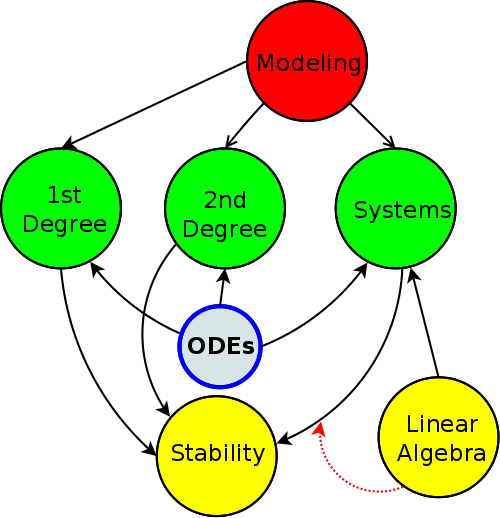
\includegraphics[height=12em]{img/topics}}
\end{frame}


\begin{frame}
  \frametitle{What is a DE?}

  Given
  \begin{eqnarray*}
    y'(x) & = & y(x),
  \end{eqnarray*}
  what is $y(x)=?$

  \begin{eqnarray*}
    \deriv{y(x)}{x} & = & y(x)
  \end{eqnarray*}

\end{frame}


\begin{frame}{Question:}
  Given
  \begin{eqnarray*}
    y'' + 3y' +2y & = & 0
  \end{eqnarray*}

  what is $y(x)$?

  \uncover<2->{
    Note: we leave often leave off the function notation.
    }

  \uncover<3->{
    Why? We are lazy!
    }

\end{frame}

\begin{frame}
  \frametitle{Notation}
  \begin{eqnarray*}
    \dot{y} & = & \deriv{y}{t} \\
    \only<2->{\ddot{y} & = & \derivTwo{y}{t} }\\
    \only<3->{y' & = & \mathrm{depends.... usually ~~} \deriv{y(x)}{x} }\\
    \only<4->{y'' & = & \derivTwo{y(x)}{x} }
  \end{eqnarray*}
\end{frame}

\begin{frame}
  \frametitle{Nomenclature}
  
  \vfill

  $\deriv{y}{x}$ - then ``ordinary differential equation.''

  \vfill

  $\frac{\partial y}{\partial x}$ - then ``partial differential
  equation.''

  \vfill

  Order is the highest number of derivatives:
  \begin{eqnarray*}
    y'' - 3 y' + 2y & = & 0, \mathrm{second~order} \\
    y'  & = & 4y, \mathrm{first~order} 
  \end{eqnarray*}

  \vfill


\end{frame}

\subsection{Modeling}


\begin{frame}
  \frametitle{Modeling}

  Why bother?

  Many ``mathematical models'' provide a relationship between rates.

  ex: Newton's Second Law, ``$\vec{F} = m \vec{a}$'' In 1 dimension:
  \begin{eqnarray*}
    m\mathrm{~(acceleration)} & = & \sum_i \lp F \rp_i, \\
    m \ddot{x} & = & \sum_i \lp F \rp_i
  \end{eqnarray*}

  
\end{frame}


\begin{frame}
  \frametitle{Circuit}
  
  The voltage across a resistor is proportional to the current flowing
  through it.

  \only<2->
  {
    There is some number, R, where
    \begin{eqnarray*}
      V & = & IR
    \end{eqnarray*}
  }
\end{frame}

\begin{frame}
  \frametitle{Proportionality}
  
  If $a$ is proportional to $b$ then there is a constant, $k$, where 
  \begin{eqnarray*}
    a  & = & k \cdot b
  \end{eqnarray*}

  if $a$ is inversely proportional to $b$ then there is a constant $c$
  where 
  \begin{eqnarray*}
    a & = & c \frac{1}{b}
  \end{eqnarray*}
\end{frame}

\begin{frame}
  \frametitle{Example - Newton's Law of Cooling}

  The rate of change of the temperature of an object is proportional
  to the difference between the object and its surroundings (the
  ambient temperature).

  \uncover<2->
  {

    Define:
    \begin{itemize}
    \item $T(t)$ is the temperature at a time $t$.
    \item $A$ is the ambient temperature (the temperature of the
      surroundings).
    \item The rate of change of the temperature is $\frac{dT(t)}{dt}$.
    \end{itemize}

  }

  \uncover<3->
  {

    There is some constant number, $k$, where 
    \begin{eqnarray*}
      \frac{dT(t)}{dt} & = & -k (T-A).
    \end{eqnarray*}

  }


\end{frame}


\begin{frame}
  \frametitle{Newton's Law of Cooling}

  The rate of change of the temperature of an object is proportional
  to the difference between the object and its surroundings (the
  ambient temperature).

    There is some constant number, $k$, where 
    \begin{eqnarray*}
      \frac{dT(t)}{dt} & = & -k (T-A).
    \end{eqnarray*}

    Question: What is the temperature at any given time?

\end{frame}


\begin{frame}{Extra Topic (Outside of class) }

  Checking your solution:
  \begin{itemize}
  \item You have a differential equation.
  \item You have a function that you think is the solution.
  \end{itemize}

  How do you check to see if it is correct?

  \uncover<2>{\color{red} You plug it back into the equation!}

  \uncover<3>{This is something that causes a large amount of
    confusion. If you are asked to \textbf{check} a solution you only
    need to plug it back into the equation and see if the
    \blueText{left side} is equal to the \fuchsiaText{right side} of
    the equation. This also means that you can always check your work
    using the skills you learned in Calculus I.}
  
\end{frame}


\begin{frame}{Example}

  Show that {\color{red} $y=t\cos(t)$} is a solution to the differential equation
  \begin{eqnarray*}
    \blueText{y' - \frac{1}{t}y} & = & \fuchsiaText{-t\sin(t)}.
  \end{eqnarray*}

  \only<2>{

    \begin{itemize}
    \item We will take the necessary derivatives of the function. (In this
      case one.)
    \item We will plug it into the equation.
    \item We will check to see if the \blueText{left hand side} is
      equal to the \fuchsiaText{right hand side}.
    \end{itemize}

  }

  \only<3-5>{

    \begin{eqnarray*}
      \redText{y} & = & \redText{t\cos(t)}, \\
      y' & = & \cos(t) - t\sin(t).
    \end{eqnarray*}
  }

  \only<4->{

    Plug the result into the left hand side of the equation:
    \begin{eqnarray*}
      \blueText{y' - \frac{1}{t}y} & = & \cos(t) - t\sin(t) - \frac{1}{t} t \cos(t), \\
      & = & \cos(t) - t\sin(t) - \cos(t), \\
      & = & -t\sin(t).
    \end{eqnarray*}

  }

  \only<5->{

    Plug the result into the right hand side of the equation (easy in
    this case!):
    \begin{eqnarray*}
      \fuchsiaText{-t\sin(t)}.
    \end{eqnarray*}

  }

  \only<6->{

    Note the result.... They are the same! The function satisfies the
    differential equation so it is \textbf{a} solution. Note that if
    there had been extra conditions we would have to check
    \textbf{all} of them.

  }
  
\end{frame}


% LocalWords:  Clarkson pausesection hideothersubsections sectionstyle Yao
% LocalWords:  Guangming ResponseCard Webwork moodle

\part{Solutions-to-DEs}
\lecture{Solutions to DEs}{Solutions-to-DEs}
\section{Solutions to DEs}

\title{Ordinary Differential Equations}
\subtitle{Math 232 - Week 1, Day 2}
\date{27 Aug 2014}

\begin{frame}
  \titlepage
\end{frame}

\begin{frame}
  \frametitle{Outline}
  \tableofcontents[ currentsection ]
\end{frame}


\subsection{Solutions to DEs}


\begin{frame}
  \frametitle{What is a solution to a DE?}

  \begin{eqnarray*}
    y' & = & y
  \end{eqnarray*}

   \uncover<2->{
     Solution: $y=3e^t$
   }

  \uncover<3->{

    {\color{red}How do you check?}
    \begin{itemize}
    \item Substitute into the left hand side.
    \item Substitute into the right hand side.
    \item See if they are the same.
    \end{itemize}

  }

  \uncover<4->{
    {\color{orange}Check:} 
    \begin{eqnarray*}
      \text{left hand side: } y' & = & 3e^t \\
      \text{right hand side: } y  & = & 3e^t
    \end{eqnarray*}

    The same! So $y=3e^t$ is {\color{red}a} solution to the DE $y'=y$
  }

\end{frame}


\begin{frame}
  \frametitle{What is a solution to a DE?}

  \begin{eqnarray*}
    y' & = & y
  \end{eqnarray*}

  Solution: $y=2e^t$

  \uncover<2->{
    Check: 
    \begin{eqnarray*}
      y' & = & 2e^t \\
      y  & = & 2e^t
    \end{eqnarray*}

    The same! So $y=2e^t$ is {\color{red}\textbf{a}} solution to the DE $y'=y$
  }


\end{frame}


\begin{frame}
  \frametitle{What is a solution to a DE?}

  \begin{eqnarray*}
    y' & = & y, \\
    y(0) & = & 4
  \end{eqnarray*}

  Neither $y = 3e^t$ nor $y=2e^t$ is a solution! 

  \uncover<2->{
    Solution: $y=4e^t$

    Check: 
    \begin{eqnarray*}
      y' & = & 4e^t \\
      y  & = & 4e^t \\
      y(0) & = & 4
    \end{eqnarray*}

    This is {\color{red}\textbf{the}} solution.
  }

\end{frame}


\begin{frame}
  \frametitle{What is a solution to a DE?}

  Show that 
  \begin{eqnarray*}
    y & = & 3 e^{2t} - \half
  \end{eqnarray*}
  is a solution to
  \begin{eqnarray*}
    y' & = & 2y + 1.
  \end{eqnarray*}

  \uncover<2->{
    \begin{eqnarray*}
      y' & = & 6 e^{2t} \\
      2y+1 & = & 2(3 e^{2t} - \half) +1 \\
      & = & 6 e^{2t}
    \end{eqnarray*}
  }


\end{frame}


\begin{frame}
  \frametitle{What is a solution to a DE?}

  Show that 
  \begin{eqnarray*}
    y & = & \half e^{2t} - \half
  \end{eqnarray*}
  is a solution to
  \begin{eqnarray*}
    y' & = & 2y + 1, \\
    y(0) & = & 0.
  \end{eqnarray*}

  \uncover<2->{
    \begin{eqnarray*}
      y' & = & e^{2t} \\
      2y+1 & = & 2\lp\half e^{2t} - \half\rp +1 \\
      & = & e^{2t} \\
      y(0) & = & \half e^0 - \half \\
      & = & 0
    \end{eqnarray*}
  }



\end{frame}


\subsection{Slope Fields}

\begin{frame}
  \frametitle{What is the derivative?}

  The derivative is the slope of the tangent line.

  \vfill
  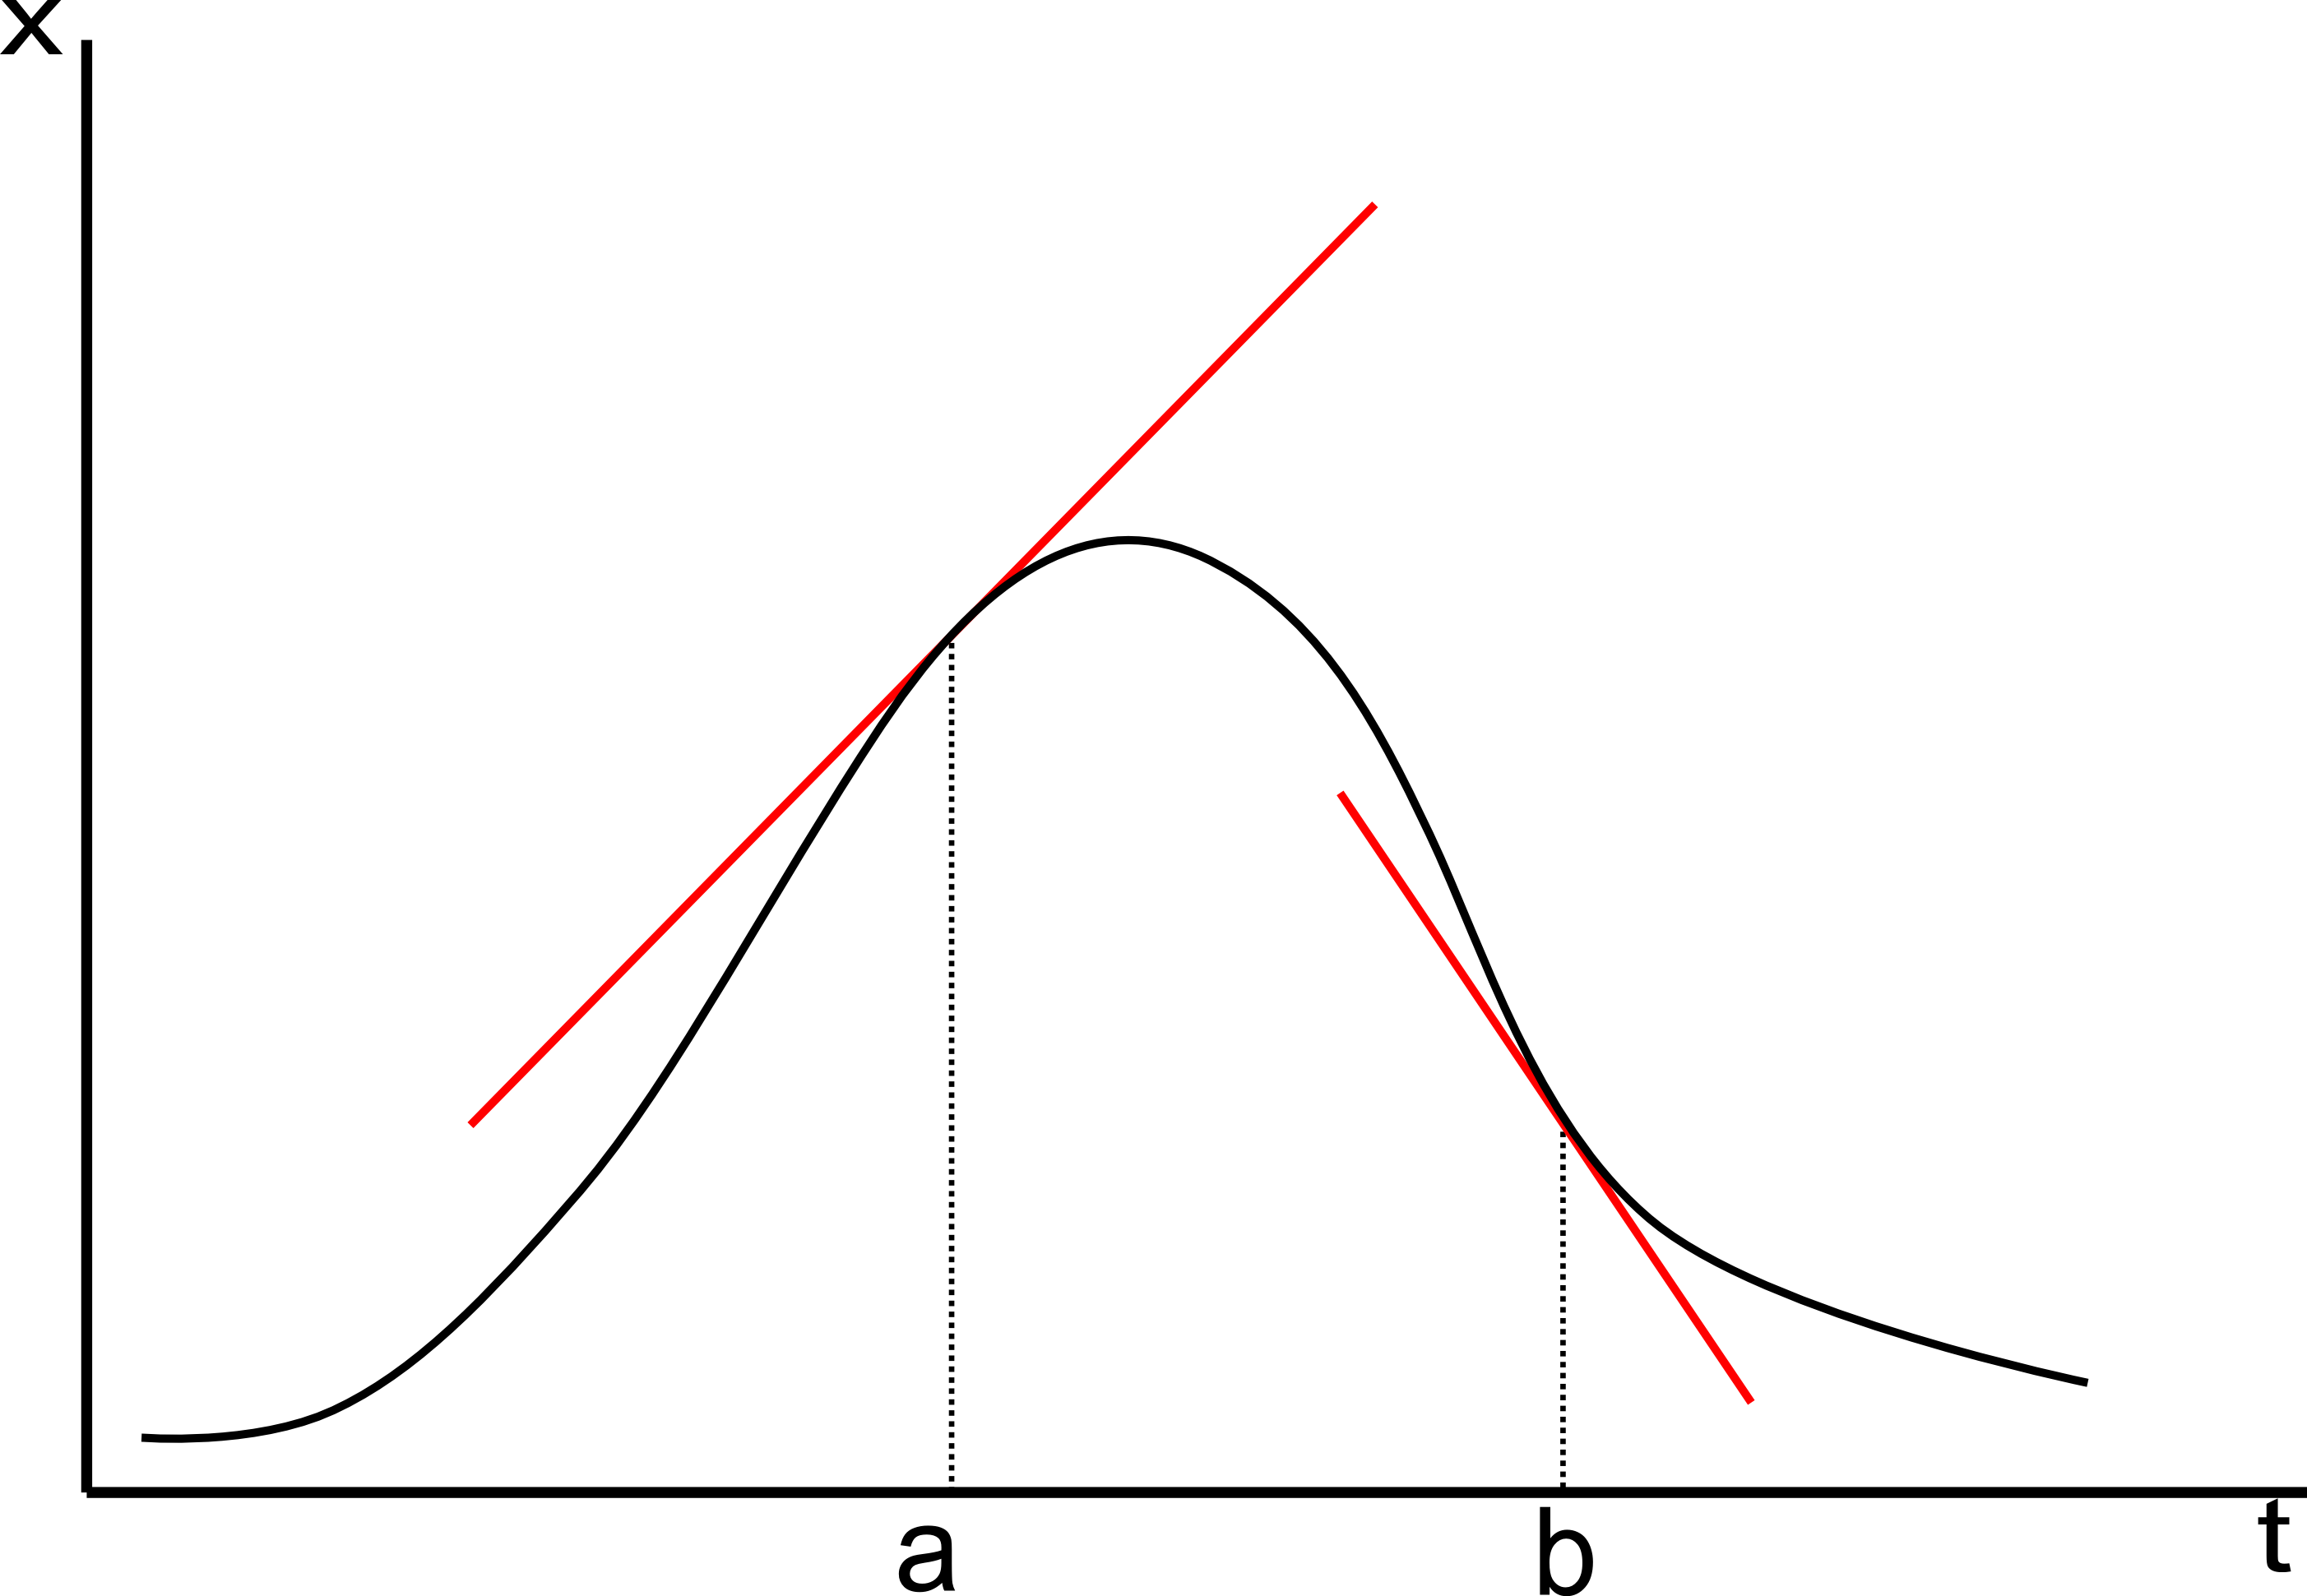
\includegraphics[height=4cm]{img/simpleSlope}
  \vfill

  \begin{tabular}{lll}
    if y'=2 & slope=2   & (increasing) \\
    if y'=3 & slope=3   & (increasing) \\
    if y'=-2 & slope=-2 & (decreasing) \\
  \end{tabular}


\end{frame}


\begin{frame}
  \frametitle{Example}

  \begin{eqnarray*}
    y' & = & 5t + 3, \\
    \int y' ~ dt & = & \int 5t + 3 ~ dt \\
    \uncover<2->{y & = & \frac{5}{2} t^2 + 3t + C}
  \end{eqnarray*}

  \uncover<2->{We get a ``family of solutions.'' }

  \uncover<3->{
    If $y(0)=2$ then
    \begin{eqnarray*}
      y(0) & = & \frac{5}{2} (0)^2 + 3(0) + C, \\
      2    & = & C
    \end{eqnarray*}
  }


\end{frame}


\begin{frame}
  \frametitle{Slope Fields}

  Given the differential equation can we predict the {\color{red}\textit{general
    behavior}} of the solution? (Qualitative behavior)

  If we have 
  \begin{eqnarray*}
    y' & = & f(t,y),
  \end{eqnarray*}
  then if we know that the function goes through a point, $t=a$ and
  $y(a)=v$, then we can calculate the slope of the tangent line.

\end{frame}


\begin{frame}
  \frametitle{Slope Fields}

  \includegraphics<1| handout:1>[height=8cm]{img/singlePointInSlopeField}

  \includegraphics<2| handout:2>[height=8cm]{img/singlePointWithSlopeField}

\end{frame}

\begin{frame}{Clicker Quiz \redText{Example}}

  \redText{(Example of a clicker quiz.)}

  Suppose that we know that the solution to the differential equation
  \begin{eqnarray*}
    y' & = & y-t
  \end{eqnarray*}
  is 6 when $t=2$. What is the slope of the tangent line at $t=2?$

     \vspace{2em}
     \begin{tabular}{ll}
       A: & 6 \\ [12pt]
       B: & 4 \\ [12pt]
       C: & 6t-6 \\ [12pt]
       D: & 4t-2 \\ [12pt]
     \end{tabular}

  
\end{frame}


\begin{frame}
  \frametitle{Example}

  \vspace*{-4em}

  \begin{eqnarray*}
    y' & = & 2y
  \end{eqnarray*}

  At $t=3$ if you happen to know that $y=4$ then the slope is 2(4)=8.

  At $t=3$ if you happen to know that $y=5$ then the slope is 2(5)=10.

  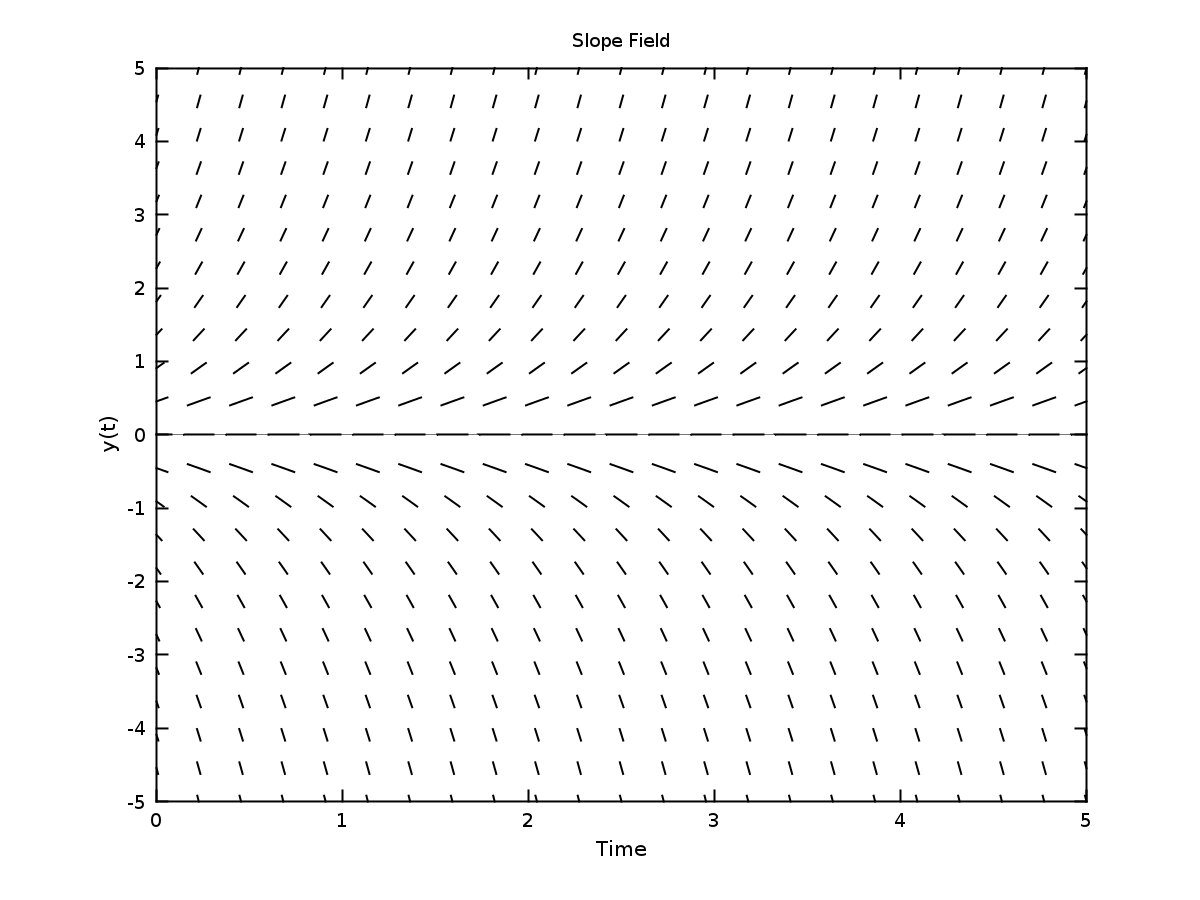
\includegraphics[height=4cm]{img/week1Day2SlopeField}

  {\color{red}A direction field (or slope field) is a collection of 
  segments that indicate the tangent lines.} 
  
\end{frame}


\begin{frame}
  \frametitle{Example}

  \vspace*{-4em}

  \begin{eqnarray*}
    y' & = & y - t
  \end{eqnarray*}

  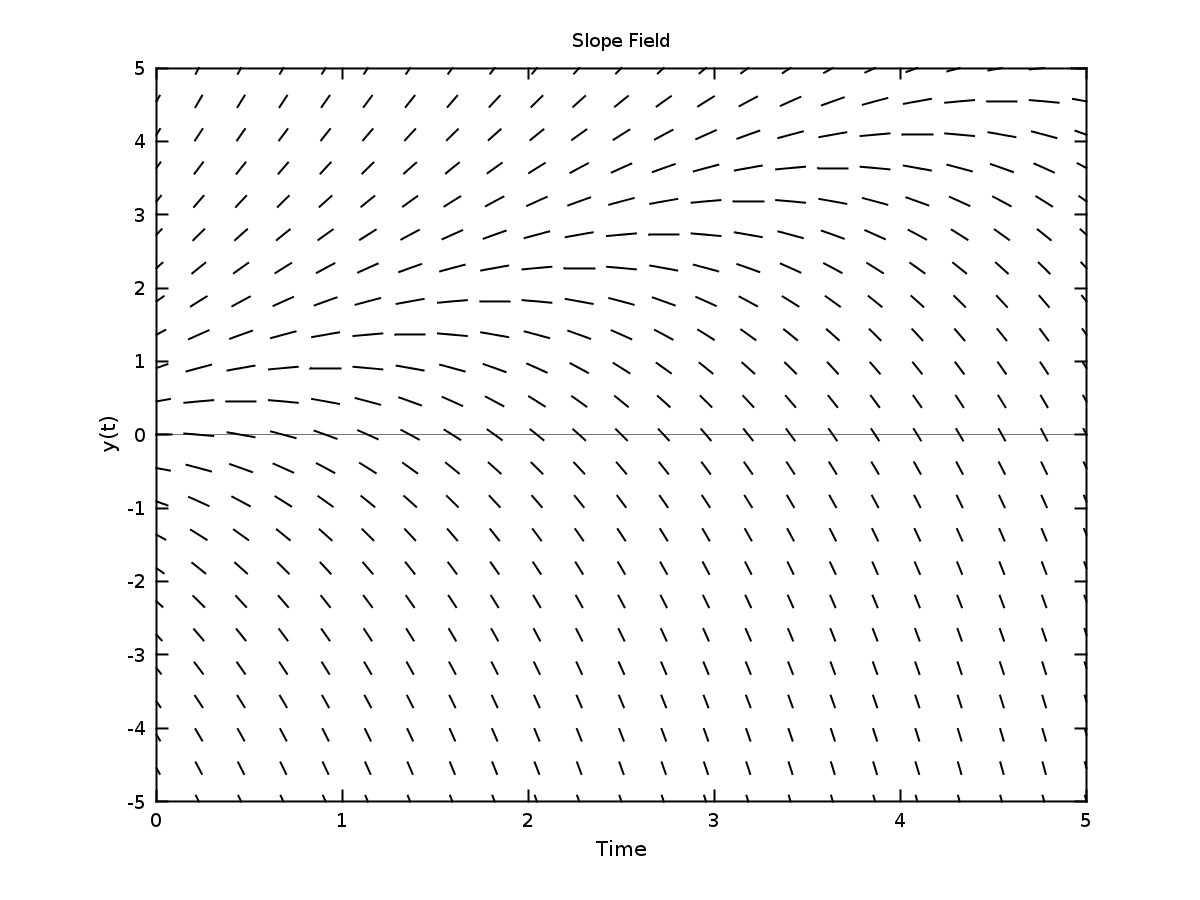
\includegraphics[height=5cm]{img/week1Day2SlopeField2}

  Tools:
  \begin{itemize}
  \item A ``{\color{red}stationary point}'' is a point where $y'=0$.
  \item An {\color{red}isocline} is a curve where $y'$ is equal to a constant.
  \end{itemize}

\end{frame}


\begin{frame}
  \frametitle{Example}

  \vspace*{-4em}

  \begin{eqnarray*}
    y' & = & y^2 - 3y
  \end{eqnarray*}

  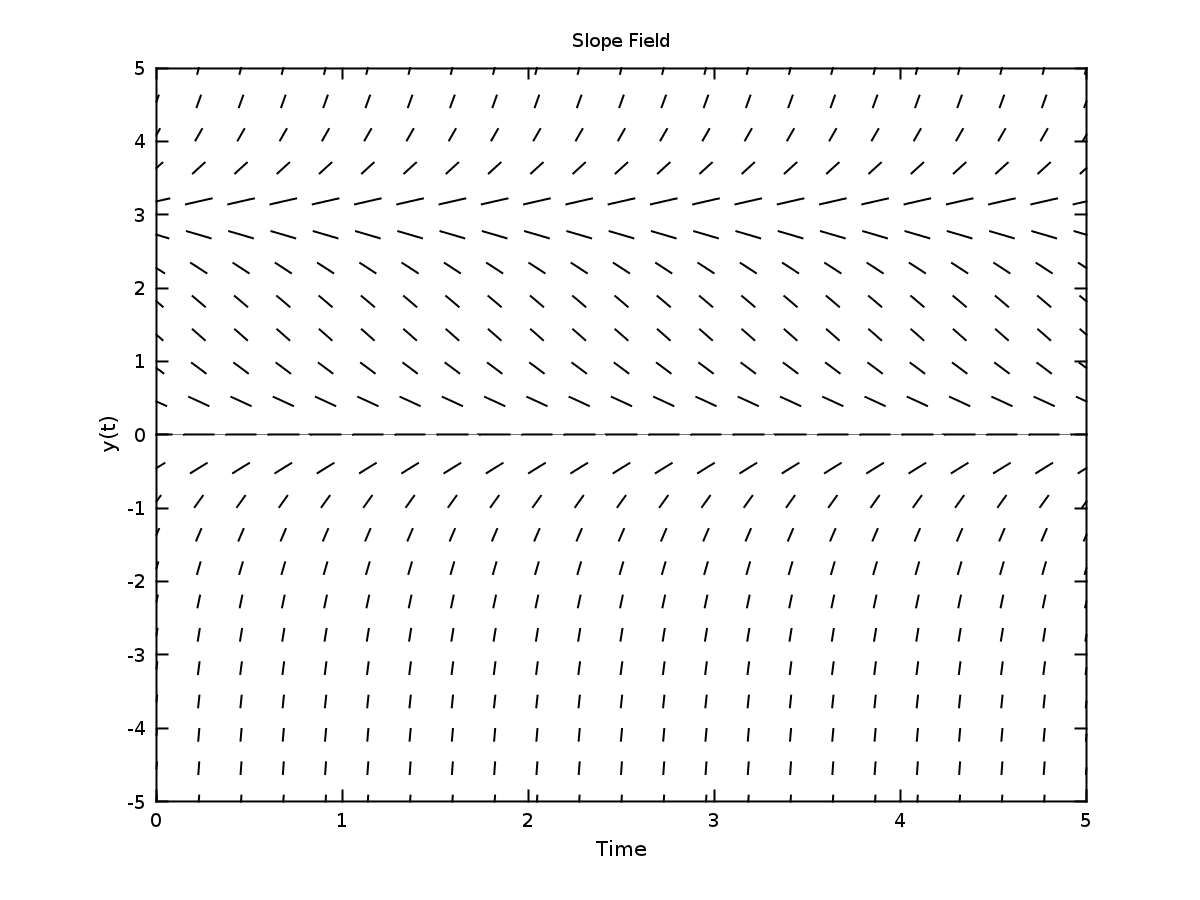
\includegraphics[height=5cm]{img/week1Day2SlopeField3}

  {\color{red}Definition: An equilibrium solution is a value for which the
  solution does not change in time.}

  \uncover<2->{$y(t)=0$ and $y(t)=3$ are equilibrium solutions.}

\end{frame}

\subsection{Stability}

\begin{frame}
  \frametitle{Stability}

  \begin{itemize}
  \item An \textit{equilibrium solution} is {\color{red}\textbf{stable}} if values
    of the solution tend to stay close to it as $t$ increases.
  \item An \textit{equilibrium solution} is {\color{red}\textbf{unstable}} if
    values of the solution tend to move away from it as $t$ increases.
  \end{itemize}

  In the previous example $y=0$ is stable while $y=3$ is unstable.

\end{frame}



% LocalWords:  Clarkson pausesection hideothersubsections isocline DEs




% %%%%%%%%%%%%%%%%%%%%%%%%%%%%%%%%%%%%%%%%%%%%%%%%%%%%%%%%%%%%
% Methods to solve and classify select differential equations

\part{Separable-Equations}
\lecture{Separable Equations}{Separable-Equations}
\section{Separable Equations}


\title{Ordinary Differential Equations}
\subtitle{Math 232 - Week 1, Day 3}
\date{30 August 2013}

\begin{frame}
  \titlepage
\end{frame}

\begin{frame}
  \frametitle{Outline}
  \tableofcontents[pausesection,hideothersubsections]
\end{frame}


\subsection{The Chain Rule}

\begin{frame}
  \frametitle{Clicker Quiz}
    \iftoggle{clicker}{%
   
      \ifnum\value{clickerQuiz}=1%

       Which function is a solution to the differential equation
       \begin{eqnarray*}
         y' & = & y\sin(t)?
       \end{eqnarray*}

       \vfill

       \begin{tabular}{l@{\hspace{3em}}l}
         A: & $y=e^{-\sin(t)}$. \\
         B: & $y=e^{\sin(t)}$. \\
         C: & $y=e^{-\cos(t)}$. \\
         D: & $y=e^{\cos(t)}$. \\
       \end{tabular}
     \fi

      \ifnum\value{clickerQuiz}=2%
       Which function is a solution to the differential equation
       \begin{eqnarray*}
         y' & = & y\cdot t?
       \end{eqnarray*}

       \vfill

       \begin{tabular}{l@{\hspace{3em}}l}
         A: & $y=e^{\half t^2}$. \\
         B: & $y=e^{t^2}$. \\
         C: & $y=e^{2 t}$. \\
         D: & $y=e^{t}$. \\
       \end{tabular}
      \fi

      \ifnum\value{clickerQuiz}=3%
       Which function is a solution to the differential equation
       \begin{eqnarray*}
         y' & = &  y\sin(t)?
       \end{eqnarray*}

       \vfill

       \begin{tabular}{l@{\hspace{3em}}l}
         A: & $y=3e^{-\sin(t)}$. \\
         B: & $y=2e^{\sin(t)}$. \\
         C: & $y=4e^{-\cos(t)}$. \\
         D: & $y=7e^{\cos(t)}$. \\
      \end{tabular}
      \fi

    \vfill
    \vfill
    \vfill

}

\end{frame}




\begin{frame}
  \frametitle{Finding Solutions}

  How do we find a solution to a DE?

  \uncover<2->{Depends!}


\end{frame}


\begin{frame}
  \frametitle{The Chain Rule}

  \begin{eqnarray*}
    \int \lp 1 + \ln(t) \rp \frac{1}{t} ~ dt & = & ?
  \end{eqnarray*}

  \uncover<2->{
    Let $u=1+\ln(t)$ then $du=\frac{1}{t}dt.$
  }

  \uncover<3-> {
    \begin{eqnarray*}
      \int \lp 1 + \ln(t) \rp \frac{1}{t} ~ dt & = & \int u ~ du \\
      & = & \half u^2 + C \\
      & = & \half \lp 1+\ln(t) \rp^2 + C
    \end{eqnarray*}
  }


\end{frame}

\begin{frame}
  \frametitle{The Chain Rule}

  \begin{eqnarray*}
    \int \lp 1 + \ln(t) \rp \frac{1}{t} ~ dt & = & ?
  \end{eqnarray*}

  \uncover<2->{
    Let $y=1+\ln(t)$ then $dy=\frac{1}{t}dt.$
  }

  \uncover<3-> {
    \begin{eqnarray*}
      \int \lp 1 + \ln(t) \rp \frac{1}{t} ~ dt & = & \int y ~ dy \\
      & = & \half y^2 + C \\
      & = & \half \lp 1+\ln(t) \rp^2 + C
    \end{eqnarray*}
  }


\end{frame}

\begin{frame}
  \frametitle{The Chain Rule}
  \begin{eqnarray*}
    \int f(y) y' ~ dt & = & \int f(y) ~ dy
  \end{eqnarray*}

  So what?

\end{frame}


\begin{frame}
  \frametitle{A Differential Equation}
  
  \begin{eqnarray*}
    y' & = & 2y
  \end{eqnarray*}

  What is $y$?

  \uncover<2->{
    Note:
    \begin{eqnarray*}
      \frac{1}{y} y' & = & 2
    \end{eqnarray*}

    The left side looks like $($function of $y)$ times $y'$.

    The right side is solely a function of $t$.

  }

\end{frame}

\subsection{Separable Equations}

\begin{frame}
  \frametitle{Separable Equations}

  Definition: A \textbf{separable differential equation} is an
  equation that can be expressed in the form 
  \begin{eqnarray*}
    y' & = & f(t) g(y).
  \end{eqnarray*}

  In our example:
  \begin{eqnarray*}
    y' & = & 2y \\
    f(t) & = & 2 \\
    g(y) & = & y
  \end{eqnarray*}

\end{frame}


\begin{frame}
  \frametitle{Solving Our Example}

  \begin{eqnarray*}
    y' & = & 2y \\
    \frac{1}{y} y' & = & 2, \\
    \uncover<2->{
      \int \frac{1}{y} y' ~ dt & = & \int 2 ~ dt \\
      \int \frac{1}{y} ~ dy & = & \int 2 ~ dt } \\
    \uncover<3->{
      \ln(y) & = & 2t + C } \\
    \uncover<4->{
      y & = & e^{2t + C} \\
      y & = & e^{2t} \cdot e^C \\
      y & = & k e^{2t}
    }
  \end{eqnarray*}

\end{frame}


\begin{frame}
  \frametitle{In General}

  \begin{eqnarray*}
    y' & = & f(t) g(y) \\
    \frac{1}{g(y)} y' & = & f(t) \\
    \int \frac{1}{g(y)} y' ~ dt & = & \int f(t) ~ dt \\
    \int \frac{1}{g(y)} ~ dy & = & \int f(t) ~ dt 
  \end{eqnarray*}

  \begin{itemize}
  \item Solve the integrals
  \item Solve for $y$ (if possible)
  \end{itemize}


\end{frame}


\begin{frame}
  \frametitle{Example}

  \begin{eqnarray*}
    y' & = & \frac{t}{y+y^2} \\
    \uncover<2->{
      \lp y + y^2 \rp y' & = & t } \\
    \uncover<3->{
      \int \lp y + y^2 \rp y' ~ dt & = & \int t ~ dt \\
      \int \lp y + y^2 \rp ~ dy & = & \int t ~ dt } \\
    \uncover<4->{
      \half y^2 + \frac{1}{3} y^3 & = & \half t^2 + C
    }
  \end{eqnarray*}

  \uncover<5->{
    Cannot solve explicitly for $y(t)$!
  }

\end{frame}


\begin{frame}
  \frametitle{Example}

  \begin{eqnarray*}
    y' & = & 3y + t
  \end{eqnarray*}

  \uncover<2-> { Not separable! }

\end{frame}


\begin{frame}
  \frametitle{Example}

  \begin{eqnarray*}
    y' & = & y^2 + 1 \\
    \uncover<2->{
      \frac{1}{y^2 + 1} y' & = & 1 } \\
    \uncover<3->{
      \int \frac{1}{y^2 + 1} y' ~ dt  & = & \int 1 ~ dt \\
      \int \frac{1}{y^2 + 1}  ~ dy  & = & \int 1 ~ dt } \\
    \uncover<4->{
      \arctan(y) & = & t + C } \\
    \uncover<5->{
      y & = & \tan(t+C)}
  \end{eqnarray*}

\end{frame}


\begin{frame}
  \frametitle{Example}

  \begin{eqnarray*}
    y' & = & yt + t \\
    \uncover<2->{
      y' & = & t(y+1) }\\
    \uncover<3->{
      \int \frac{1}{y+1} y' ~ dt & = & \int t ~ dt \\
      \int \frac{1}{y+1} ~ dy & = & \int t ~ dt \\
    }
    \uncover<4->{
      \ln(y+1) & = & \half t^2 + C }\\
    \uncover<5->{
      y+1 & = & e^{\half t^2 + C} \\
      y+1 & = & e^{\half t^2}e^{C} \\
      y+1 & = & k e^{\half t^2} \\
      y = ke^{\half t^2} - 1 }
  \end{eqnarray*}

\end{frame}


\begin{frame}
  \frametitle{Example}

  \begin{eqnarray*}
    y' & = & \cos(ty) 
  \end{eqnarray*}

  \uncover<2->{Not Separable!}

\end{frame}




\begin{frame}
    \iftoggle{clicker}{%
      \frametitle{Clicker Quiz}
    
      \ifnum\value{clickerQuiz}=1%
      Find the general solution to the equation
       \begin{eqnarray*}
         y' & = & y^2t.
       \end{eqnarray*}

       \vfill

       \begin{tabular}{l@{\hspace{3em}}l}
         A: & $\lp\half t^2\rp^{1/3} +C$. \\ [10pt]
         B: & $\sqrt[3]{\half t^2+C}$. \\  [10pt]
         C: & $e^{\half t^2 + C}$. \\   [10pt]
         D: & $\frac{-1}{\half t^2 + C}$. \\  [10pt]
       \end{tabular}

    \fi

    \ifnum\value{clickerQuiz}=2%
       Find the general solution to the equation
       \begin{eqnarray*}
         y' & = & \frac{1}{yt}.
       \end{eqnarray*}

       \vfill

       \begin{tabular}{l@{\hspace{3em}}l}
         A: & $y=\pm\sqrt{2\ln(t)}+C$. \\ [10pt]
         B: & $y=\pm\sqrt{2\ln(t)+C}$. \\  [10pt]
         C: & $y=t+C$. \\   [10pt]
         D: & $y=\ln(t)+C$. \\  [10pt]
       \end{tabular}

    \fi

    \ifnum\value{clickerQuiz}=3%
       Find the general solution to the equation
       \begin{eqnarray*}
         y' & = & -2t^2y?
       \end{eqnarray*}

       \vfill

       \begin{tabular}{l@{\hspace{3em}}l}
         A: & $e^{\frac{-2t^3}{3}}+C$. \\ [10pt]
         B: & $-\dfrac{2t^3}{3}+C$. \\  [10pt]
         C: & $\sqrt[3]{\half t^2+C}$. \\   [10pt]
         D: & $e^{\frac{-2t^3}{3}+C}$. \\  [10pt]
       \end{tabular}

    \fi

    \vfill
    \vfill
    \vfill

}

\end{frame}

\begin{frame}
  \frametitle{Example}

  \begin{eqnarray*}
    y' & = & \frac{t}{y}, ~~~ y(0)=2 \\
    \uncover<2->{
      y y' & = & t } \\
    \uncover<3->{
      \int y y' ~ dt & = & \int t ~ dt } \\
    \uncover<4->{
      \half y^2 & = & \half t^2 + C \\
      y^2 & = & t^2 + k } \\
    \uncover<5->{
      2^2 & = & 0 + k \\
      k   & = & 4 \\
      y & = & \pm \sqrt{t^2+4} } \\
    \uncover<6->{
      \mathrm{Must ~ be ~ positive!} \\
      y & = & \sqrt{t^2+4} }
  \end{eqnarray*}

  \uncover<6->{
    See example 4 in the book.
  }

\end{frame}


\begin{frame}
  \frametitle{Example}

  \begin{eqnarray*}
    ty' & = & y^2 t^2 + 1 \\
    \uncover<2->{
      y'  & = & y^2 t + \frac{1}{t} }
  \end{eqnarray*}

  \uncover<3->{Not separable!}

\end{frame}


\begin{frame}
  \frametitle{Example}

  \begin{eqnarray*}
    t y' & = & y^2+1 \\
    \uncover<2->{
      \frac{y'}{y^2+1} & = & \frac{1}{t} } \\
    \uncover<3->{
      \int \frac{y'}{y^2+1} ~ dt & = & \int \frac{1}{t} ~ dt \\
      \int \frac{1}{y^2+1} ~ dy & = & \int \frac{1}{t} ~ dt } \\
    \uncover<4->{
      \arctan(y) & = & \ln(t)+C } \\
    \uncover<5->{
      y & = & \tan(\ln(t)+C)}
  \end{eqnarray*}





\end{frame}


\begin{frame}
  \frametitle{Example}

  \vspace*{-3em}
  \begin{eqnarray*}
    y' & = & \sec(y) t^2 + \sec(y) \sin(4t) \\
    \uncover<2->{
      y' & = & \sec(y) \lp t^2 + \sin(4t) \rp } \\
    \uncover<3->{
      \frac{y'}{\sec(y)} & = & t^2 + \sin(4t) } \\
    \uncover<4->{
      \int \frac{y'}{\sec(y)} ~ dt & = & \int t^2 + \sin(4t) ~ dt \\
      \int \frac{1}{\sec(y)} ~ dy & = & \int t^2 + \sin(4t) ~ dt }\\
    \uncover<5->{
      \int \cos(y) ~ dy & = & \int t^2 + \sin(4t) ~ dt } \\ 
    \uncover<6->{
      \sin(y) & = & \frac{1}{3} t^3 - \frac{1}{4} \cos(4t) + C } \\
    \uncover<7->{
      y & = & \arcsin\lp\frac{1}{3} t^3 - \frac{1}{4} \cos(4t) + C\rp } \\
  \end{eqnarray*}

  \uncover<8->{This is problematic!}

\end{frame}
 


% LocalWords:  Clarkson pausesection hideothersubsections dt dy du

\part{Linear-Equations}
\lecture{Linear Equations}{Linear-Equations}
\section{Linear Equations}


\title{Ordinary Differential Equations}
\subtitle{Math 232 - Week 2, Day 1}
\date{3 Sep 2012}

\begin{frame}
  \titlepage
\end{frame}

\begin{frame}
  \frametitle{Outline}
  \tableofcontents[pausesection,hideothersubsections]
\end{frame}


\subsection{Linear Equations}


\iftoggle{clicker}{%
\begin{frame}
  \frametitle{Clicker Quiz}
    
      \ifnum\value{clickerQuiz}=1{%

       Determine the solution to the differential equation
       \begin{eqnarray*}
         y' & = & y + 1.
       \end{eqnarray*}

       \vfill

       \begin{tabular}{l@{\hspace{3em}}l}
         A: & $y=-1 + e^t + C$. \\
         B: & $y=-1+ke^t$. \\
         C: & $y=ke^t$. \\
         D: & $y=1+ke^t$. \\
       \end{tabular}
     }\fi

     \ifnum\value{clickerQuiz}=2{%
       Determine the solution to the differential equation
       \begin{eqnarray*}
         y' & = & ty.
       \end{eqnarray*}

       \vfill

       \begin{tabular}{l@{\hspace{3em}}l}
         A: & $y=\half ke^{t^2}$. \\
         B: & $y=ke^{t}$. \\
         C: & $y=ke^{t^2/2}$. \\
         D: & $y=e^{t^2/2} + C$. \\
       \end{tabular}
     }\fi

      \ifnum\value{clickerQuiz}=3{%
       Determine the solution to the differential equation
       \begin{eqnarray*}
       y' & = & -2t^2y? 
       \end{eqnarray*}

       \vfill

       \begin{tabular}{l@{\hspace{3em}}l}
         A: & $y=e^{\frac{-2t^3}{3}}+C$. \\
         B: & $y=-\dfrac{2t^3}{3}+C$. \\
         C: & $y=\sqrt[3]{\half t^2+C}$. \\
         D: & $y= k e^{\frac{-2t^3}{3}}$. \\
       \end{tabular}
     }\fi

    \vfill
    \vfill
    \vfill

\end{frame}
}



\begin{frame}
  \frametitle{Linear Equations}

  If we have variables $x_1$, $x_2$, \ldots, $x_n$ then an equation of
  the form
  \begin{eqnarray*}
    a_1 x_1 + a_2 x_2 + \cdots + a_n x_n & = & c,
  \end{eqnarray*}
  where $a_1$, $a_2$, \ldots, $a_n$, and $c$ are constants, is a
  \textbf{linear equation}.

  if $c$ is zero the equation is \textbf{homogeneous}.

\end{frame}


\begin{frame}
  \frametitle{Linear Equations}

  \begin{eqnarray*}
    3 x_1 + 4 x_2 = 5 & & \uncover<2->{\mathrm{Linear}} \\
    3 x_1 + 4 x^3_2 = 5 & & \uncover<3->{\mathrm{Not~Linear}} \\
    3 \sqrt{x_1} + 4 x_2 = 5 & & \uncover<4->{\mathrm{Not~Linear}} \\
  \end{eqnarray*}


\end{frame}


\begin{frame}
  \frametitle{Linear Differential Equations}

  In the context of DEs an equation is linear if it is in the form
  \begin{eqnarray*}
    a_0(t) y(t) + a_1(t) \frac{d}{dt}y(t) + \cdots +
    a_n(t) \frac{d^n}{dt^n}y(t) & = & f(t).
  \end{eqnarray*}

  if $f(t)$ is zero the equation is \textbf{homogeneous}.

\end{frame}


\begin{frame}
  \frametitle{Example}

  \vspace*{-3em}
  \begin{eqnarray*}
    3t y + y' - \sin(t) y'' & = & \ln(t)
  \end{eqnarray*}
  \centerline{\color{red}{\uncover<2->{Linear, variable coefficients, nonhomogeneous!}}}

  \begin{eqnarray*}
    3t \sqrt{y} + y' - \sin(t) y'' & = & \ln(t)
  \end{eqnarray*}
  \centerline{\color{red}{\uncover<3->{Not Linear, variable coefficients, nonhomogeneous!}}}

  \begin{eqnarray*}
    3 y' -y'' & = & 4 y
  \end{eqnarray*}
  \centerline{\color{red}{\uncover<4->{Linear, constant coefficients, homogeneous!}}}
  \centerline{\uncover<5->{Linear, \textbf{constant coefficient}, and homogeneous}}

  Recognizing the form is the hardest part!

\end{frame}

\subsection{Solutions to Differential Equations}

\begin{frame}
  \frametitle{Solutions to Differential Equations}

  If an equation is linear and homogeneous then:
  \begin{itemize}
  \item If $y_1(t)$ is a solution, and
  \item if $y_2(t)$ is a solution
  \end{itemize}

  then,
  \begin{eqnarray*}
    y_1(t) + y_2(t)
  \end{eqnarray*}
  is a solution.

  Also if $C_1$ and $C_2$ are constants then
  \begin{eqnarray*}
    C_1 y_1(t) + C_2 y_2(t)
  \end{eqnarray*}
  is also a solution.

  Because:
  \begin{eqnarray*}
    \frac{d}{dt} \lp C_1 y_1(t) + C_2 y_2(t) \rp & = &
    C_1 y_1'(t) + C_2 y_2'(t)
  \end{eqnarray*}


\end{frame}


\begin{frame}
  \frametitle{Example}

  Solutions to the second order equation,
  \begin{eqnarray*}
    y'' + y & = & 0,
  \end{eqnarray*}
  are
  \begin{eqnarray*}
    y_1(t) & = & \cos(t) \\
    y_2(t) & = & \sin(t).
  \end{eqnarray*}

  \uncover<2->{%

    Because:
    \begin{eqnarray*}
      y''_1(t) & = & -\cos(t), \\
      \Rightarrow y''_1(t) + y_1(t) & = & -\cos(t)+\cos(t), \\
      y''_2(t) & = & -\sin(t), \\
      \Rightarrow y''_2(t) + y_2(t) & = & -\sin(t)+\sin(t).
    \end{eqnarray*}

  }

\end{frame}

\begin{frame}
  \frametitle{Example}

  Also:
  \begin{eqnarray*}
    y(t) & = & C_1 \cos(t) + C_2 \sin(t), \\
    y'(t) & = & -C_1 \sin(t) + C_2 \cos(t), \\
    y''(t) & = & -C_1 \cos(t) - C_2 \sin(t), \\
    y''(t) + y(t) & = & -C_1 \cos(t) - C_2 \sin(t) + C_1 \cos(t) + C_2 \sin(t) \\
    & = & 0
  \end{eqnarray*}


\end{frame}


\iftoggle{clicker}{%
\begin{frame}
  \frametitle{Clicker Quiz}
    
      \ifnum\value{clickerQuiz}=1{%

        The function $y=-2e^{3t} + 4 e^{2t}$ is a solution to the
        equation
        \begin{eqnarray*}
          y'' - 5 y' + 6y & = & 0.
        \end{eqnarray*}

        Is the function $y=5e^{3t} - e^{2t}$ also a solution?

       \vfill

       \begin{tabular}{l@{\hspace{3em}}l}
         A: & Yes, it is a solution. \\
         B: & No, it is not a solution.
       \end{tabular}

     }\fi

     \ifnum\value{clickerQuiz}=2{%

        The function $y=2e^{3t}$ is a solution to the
        equation
        \begin{eqnarray*}
          y' & = & y^2.
        \end{eqnarray*}

        Is the function $y=50e^{3t}$ also a solution?

       \vfill

       \begin{tabular}{l@{\hspace{3em}}l}
         A: & Yes, it is a solution. \\
         B: & No, it is not a solution.
       \end{tabular}

     }\fi

      \ifnum\value{clickerQuiz}=3{%
      The function $y=-\frac{1}{t+3}$ is a solution to the
        equation
        \begin{eqnarray*}
          y' & = & y^2.
        \end{eqnarray*}

        Is the function $y=\frac{2}{t+3}$ also a solution?

       \vfill

       \begin{tabular}{l@{\hspace{3em}}l}
         A: & Yes, it is a solution. \\
         B: & No, it is not a solution.
       \end{tabular}

     }\fi

    \vfill
    \vfill
    \vfill

\end{frame}
}



\subsection{Nonhomogeneous Solutions and Homogeneous Solutions}


\begin{frame}
  \frametitle{It Gets Worse!}

  Suppose that an equation is linear but not homogeneous,
  \begin{eqnarray*}
    a_0(t) y_p(t) + a_1(t) \frac{d}{dt} y_p(t) + \cdot + a_n(t) \frac{d^n}{dt^n} y_p(t) & = & f(t)
  \end{eqnarray*}
  where $f(t)$ is not zero.

  The homogeneous version is
  \begin{eqnarray*}
    a_0(t) y_h(t) + a_1(t) \frac{d}{dt} y_h(t) + \cdot + a_n(t) \frac{d^n}{dt^n} y_h(t) & = & 0.
  \end{eqnarray*}

  then $y_p(t)+y_h(t)$ is a solution to the original equation!


\end{frame}


\begin{frame}
  \frametitle{Example}

  \begin{eqnarray*}
    y' - y & = & t
  \end{eqnarray*}

  Particular: $y_p = -t-1$

  \begin{eqnarray*}
    y'_p & = & -1, \\
    -1 - (-t -1) & = & t.
  \end{eqnarray*}

  Homogeneous: $y_h = k e^t$

  \begin{eqnarray*}
    y'_h - y_h & = & 0, \\
    y'_h & = & k e^t, \\
    k e^t - k e^t & = & 0.
  \end{eqnarray*}

\end{frame}

\begin{frame}
  \frametitle{Example}

  \begin{eqnarray*}
    y' - y & = & t
  \end{eqnarray*}

  \begin{eqnarray*}
    y & = & -t - 1 + ke^t, \\
    y' & = & -1 + ke^t, \\
    -1-ke^t - (-t-1-ke^t) & = & t.
  \end{eqnarray*}

\end{frame}


\begin{frame}
  \frametitle{Example}

  \begin{eqnarray*}
    y'' + 4y & = & t.
  \end{eqnarray*}

  \begin{eqnarray*}
    y_p & = & \frac{1}{4} t, \\
    y'_p & = & \frac{1}{4}, \\
    y''_p & = & 0, \\
    0 + 4\frac{1}{4} t & = & t
  \end{eqnarray*}
\end{frame}

\begin{frame}
  \frametitle{Example - Homogeneous Part}

  \begin{eqnarray*}
    y''_h + 4y_h & = & 0, \\
    y_h & = & C_1 \cos(2t) + C_2 \sin(2t), \\
    y'_h & = & -2 C_1 \sin(2t) + 2 C_2 \cos(2t), \\
    y''_h & = & -4 C_1 \cos(2t) - 4 C_2 \sin(2t),
  \end{eqnarray*}
  \begin{eqnarray*}
    -4 C_1 \cos(2t) - 4 C_2 \sin(2t) + 4\lp C_1 \cos(2t) + C_2 \sin(2t) \rp & = & 0.
  \end{eqnarray*}

\end{frame}


\begin{frame}
  \frametitle{Example - Bring them together}

  \begin{eqnarray*}
    y & = & y_p + y_h \\
    & = & \frac{1}{4} t + C_1 \cos(2t) + C_2 \sin(2t), \\
    y' & = & \frac{1}{4} - 2 C_1 \sin(2t) + 2 C_2 \cos(2t), \\
    y'' & = & - 4 C_1 \cos(2t) - 4 C_2 \sin(2t),
  \end{eqnarray*}

  \begin{eqnarray*}
    - 4 C_1 \cos(2t) - 4 C_2 \sin(2t) + 4 \lp \frac{1}{4} t + C_1 \cos(2t) + C_2 \sin(2t) \rp & = & t
  \end{eqnarray*}

\end{frame}


\begin{frame}
  \frametitle{Example}

  \begin{eqnarray*}
    y' - 3y & = & 4
  \end{eqnarray*}

  \begin{eqnarray*}
    y_p & = & -\frac{4}{3}, \\
    y_h & = & k e^{3t}
  \end{eqnarray*}

  \begin{eqnarray*}
    y & = & -\frac{4}{3} + k e^{3t}, \\
    y' & = & 3 k e^{3t}, \\
    3 k e^{3t} - 3 \lp -\frac{4}{3} + k e^{3t} \rp & = & 4
  \end{eqnarray*}


\end{frame}


\begin{frame}
  \frametitle{Example}

  \begin{eqnarray*}
    y' - 3ty & = & t^3
  \end{eqnarray*}

  \begin{eqnarray*}
    y_p & = & -\frac{1}{3} t^2 - \frac{2}{9}, \\
    y_h & = & k e^{\frac{3}{2}t^2}
  \end{eqnarray*}

  \begin{eqnarray*}
    y & = & -\frac{1}{3} t^2 - \frac{2}{9} + k e^{\frac{3}{2}t^2} \\
    y' & = & -\frac{2}{3} t + 3t k e^{\frac{3}{2}t^2}
  \end{eqnarray*}

  Substituting back into the equation we get
  \begin{eqnarray*}
    -\frac{2}{3} t + 3t k e^{\frac{3}{2}t^2} - 3t \lp -\frac{1}{3} t^2 - \frac{2}{9} + k e^{\frac{3}{2}t^2} \rp & = & t^3.
  \end{eqnarray*}

\end{frame}



\part{First-Order-Linear-Equations}
\lecture{First Order Linear Equations}{First-Order-Linear-Equations}
\section{First Order Linear Equations}

\title{Ordinary Differential Equations}
\subtitle{Math 232 - Week 2, Day 2}
\date{3 Sep 2014}

\begin{frame}
  \titlepage
\end{frame}

\begin{frame}
  \frametitle{Outline}
  \tableofcontents[ currentsection ]
\end{frame}


\subsection{First Order Linear Equations}

\iftoggle{clicker}{%

  \begin{frame}
    \frametitle{Clicker Quiz}

      \ifnum\value{clickerQuiz}=1{%

        Which differential equation is a linear equation?

       \vfill

       \begin{tabular}{l@{\hspace{3em}}l}
         A: & $y'=y^2$. \\
         B: & $y'' + 3y'-2y=0$. \\
         C: & $y'+\sqrt{y}=\sin(t)$. \\
         D: & $y' + \cos(t)y  =  \ln(t)$. \\
         E: & A and B. \\
         F: & B and D.
       \end{tabular}

     }\fi

     \ifnum\value{clickerQuiz}=2{%

        Which differential equation is a linear equation?

       \vfill

       \begin{tabular}{l@{\hspace{3em}}l}
         A: & $y'=3y$. \\
         B: & $y'' + 3\sin(t)y'-2y=0$. \\
         C: & $y''+ y^2 =\sin(t)$. \\
         D: & $y' + y y'  =  \ln(t)$. \\
         E: & A and B. \\
         F: & A and D.
       \end{tabular}


     }\fi


      \ifnum\value{clickerQuiz}=3{%
       Which differential equation is a linear equation?
      \vfill

       \begin{tabular}{l@{\hspace{3em}}l}
         A: & $y'-y^2 = 0$. \\
\vspace{0.3cm}
         B: & $y'' + 3y'-2y=t^2$. \\
\vspace{0.3cm}
         C: & $y'+\cos{y}=\sqrt(t)$. \\
\vspace{0.3cm}
         D: & $y' + \ln(t)y  =  \cos(t)$. \\
\vspace{0.3cm}
         E: & A and B. \\
\vspace{0.3cm}
         F: & B and D.
\vspace{0.3cm}
       \end{tabular}

      }\fi

    \vfill
    \vfill
    \vfill

  \end{frame}

}


\begin{frame}
  \frametitle{First ``Special Form''}

  Separable equations:
  \begin{eqnarray*}
    y' & = & f(t) g(y).
  \end{eqnarray*}

\end{frame}


\begin{frame}
  \frametitle{Another ``Special Form''}

  \begin{eqnarray*}
    y' + p(t) y & = & f(t)
  \end{eqnarray*}

  read pages 63-66

  I will only cover integrating factors in class.

\end{frame}

\subsection{Product Rule}

\begin{frame}
  \frametitle{The Product Rule}

  \begin{eqnarray*}
    \frac{d}{dt} \lp u(t) v(t) \rp & = & u'(t) v(t) + u(t) v'(t)
  \end{eqnarray*}

  \only<2->{
    Special case, $v(t)=\redText{e^{f(t)}}$.
    \begin{eqnarray*}
      \frac{d}{dt} \lp u(t) \redText{e^{f(t)}} \rp & = &
      u'(t) \redText{e^{f(t)}} + u(t) \blueText{f'(t)} \redText{e^{f(t)}}.
    \end{eqnarray*}
  }

\end{frame}


\begin{frame}
  \frametitle{Example}

  \begin{eqnarray*}
    y ' & = & - y + t \\
    \uncover<2->{ y' + y & = & t} \\
    \uncover<3->{y' e^t + y e^ t & = & t e^t } \\
    \uncover<4->{\deriv{~}{t} \lp y e^t \rp & = & t e^t } \\
    \uncover<5->{y e^t  & = & \int t e^t ~ dt } \\
    \uncover<6->{y e^t  & = & t e^t - e^t + C } \\
    \uncover<7->{ y & = & t -1 + Ce^{-t}}
  \end{eqnarray*}

  \uncover<8->{How did I know how to do this?}


\end{frame}


\subsection{Integrating Factors}

\begin{frame}
  \frametitle{Let's Backup}

  \begin{eqnarray*}
    y' + p(t) y & = & f(t) \\
    \redText{e^{G(t)}} y' + p(t) \redText{e^{G(t)}} y & = & \redText{e^{G(t)}} f(t)
  \end{eqnarray*}


\end{frame}



\begin{frame}
  \frametitle{Product Rule Redux}

  \begin{eqnarray*}
    \frac{d}{dt} \lp \redText{e^{G(t)}} \rp & = & \blueText{G'(t)} \redText{e^{G(t)}}.
  \end{eqnarray*}

  Let
  \begin{eqnarray*}
    G'(t) & = & p(t) \\
    \Rightarrow G(t) & = & \int p(t) ~ dt.
  \end{eqnarray*}


\end{frame}


\begin{frame}
  \frametitle{Product Rule Redux}

  Remember:
  \begin{eqnarray*}
    y' + p(t) y & = & f(t)
  \end{eqnarray*}


  \begin{eqnarray*}
    \frac{d}{dt} \lp \redText{e^{G(t)}} y \rp & = & \redText{e^{G(t)}} y' + \blueText{G'(t)} \redText{e^{G(t)}} y \\
    & = & \redText{e^{G(t)}} y' + \blueText{p(t)} \redText{e^{G(t)}} y \\
    & = & \redText{e^{G(t)}} \lp y' + \blueText{p(t)} y \rp \\
    & = &  \redText{e^{G(t)}} f(t)
  \end{eqnarray*}

  or
  \begin{eqnarray*}
    e^{G(t)} y & = & \int f(t) e^{G(t)} ~ dt
  \end{eqnarray*}
  \textit{Hope and pray!}

\end{frame}


\subsection{Examples}

\begin{frame}
  \frametitle{Example}

  \vspace*{-3em}
  \begin{eqnarray*}
    y' + \blueText{2}y & = & t \\
    \uncover<2->{%
      \blueText{p(t)} & = & \blueText{2}, \\
      \int \blueText{2} ~ dt & = & 2t + K, \\
      \redText{e^{2t}} & &
      }
  \end{eqnarray*}

  \uncover<3>{%
    \begin{eqnarray*}
      \redText{e^{2t}} y' + \blueText{2} \redText{e^{2t}} y & = & t \redText{e^{2t}}, \\
      \frac{d}{dt} \lp \redText{e^{2t}} y \rp & = & t \redText{e^{2t}} \\
      \redText{e^{2t}} y & = & \int t \redText{e^{2t}} ~ dt \\
      \redText{e^{2t}} y & = & \half t e^{2t} - \frac{1}{4} e^{2t} + C \\
      y & = & \half t - \frac{1}{4} + C e^{-2t}
    \end{eqnarray*}
  }

\end{frame}


\iftoggle{clicker}{%
\begin{frame}
  \frametitle{Clicker Quiz}

      \ifnum\value{clickerQuiz}=1{%

        What is the integrating factor for the equation
        \begin{eqnarray*}
          y' & = & ty + 1 ?
        \end{eqnarray*}

       \vfill

       \begin{tabular}{l@{\hspace{3em}}l}
         A: & $e^{t}$. \\
         B: & $e^{-t}$. \\
         C: & $e^{t^2/2}$. \\
         D: & $e^{-t^2/2}$. \\
       \end{tabular}

     }\fi

     \ifnum\value{clickerQuiz}=2{%

        What is the integrating factor for the equation
        \begin{eqnarray*}
          y' & = & ty + t^4 ?
        \end{eqnarray*}

       \vfill

       \begin{tabular}{l@{\hspace{3em}}l}
         A: & $e^{t}$. \\
         B: & $e^{-t}$. \\
         C: & $e^{t^2/2}$. \\
         D: & $e^{-t^2/2}$. \\
       \end{tabular}


     }\fi

      \ifnum\value{clickerQuiz}=3{%
            What is the integrating factor for the equation
        \begin{eqnarray*}
          3 y' + y & = & 3t ?
        \end{eqnarray*}

       \vfill

       \begin{tabular}{l@{\hspace{3em}}l}
         A: & $e^{t}$. \\
         B: & $e^{-t}$. \\
         C: & $e^{t/2}$. \\
         D: & $e^{t/3}$. \\
       \end{tabular}


     }\fi

    \vfill
    \vfill
    \vfill

\end{frame}

}


\begin{frame}
  \frametitle{Example}

  \vspace*{-3em}
  \begin{eqnarray*}
    y' & = & ty + t^3 \\
    \uncover<2->{%
      y' \blueText{- t}y & = & t^3 \\
      \blueText{p(t)} & = & \blueText{-t}, \\
      \int \blueText{-t} ~ dt & = & -\half t^2 + K \\
      \redText{e^{-\half t^2}} & &
    }
  \end{eqnarray*}

  \uncover<3->{%
    \begin{eqnarray*}
      y' \redText{e^{-\half t^2}} \blueText{ - t} \redText{e^{-\half t^2}} y & = & t^3 \redText{e^{-\half t^2}} \\
      \frac{d}{dt} \lp y \redText{e^{-\half t^2}} \rp & = &  t^3 \redText{e^{-\half t^2}} \\
     y \redText{e^{-\half t^2}}  & = & \int t^3 \redText{e^{-\half t^2}} ~ dt \\
     y \redText{e^{-\half t^2}} & = & -t^2 e^{-\half t^2} - 2 e^{-\half t^2} + C \\
     y & = & -t^2 - 2 + C e^{\half t^2}
   \end{eqnarray*}
 }

\end{frame}


\iftoggle{clicker}{%
\begin{frame}
  \frametitle{Clicker Quiz}

      \ifnum\value{clickerQuiz}=1{%

        What is the integrating factor for the equation
        \begin{eqnarray*}
          y' & = & -\frac{4}{t} y + 4 ?
        \end{eqnarray*}

       \vfill

       \begin{tabular}{l@{\hspace{3em}}l}
         A: & $4t$. \\
         B: & $4\ln(t)$. \\
         C: & $t^4$. \\
         D: & $t^{-4}$. \\
       \end{tabular}

     }\fi

     \ifnum\value{clickerQuiz}=2{%

        What is the integrating factor for the equation
        \begin{eqnarray*}
          y' & = & -\frac{4}{t} y + t^3?
        \end{eqnarray*}

       \vfill

       \begin{tabular}{l@{\hspace{3em}}l}
         A: & $t^{-4}$. \\
         B: & $t^4$. \\
         C: & $4\ln(t)$. \\
         D: & $4t$. \\
       \end{tabular}


     }\fi

      \ifnum\value{clickerQuiz}=3{%
       What is the integrating factor for the equation
        \begin{eqnarray*}
          y' & = & \frac{3}{t} y + 7?
        \end{eqnarray*}

       \vfill

       \begin{tabular}{l@{\hspace{3em}}l}
         A: & $t^{-3}$. \\
         B: & $t^3$. \\
         C: & $3\ln(t)$. \\
         D: & $3t$. \\
       \end{tabular}

     }\fi

    \vfill
    \vfill
    \vfill

\end{frame}

}


\begin{frame}
  \frametitle{Example}

  \begin{eqnarray*}
    y' & = & -\frac{4}{t} y + 4 t \\
    \uncover<2->{%
      y' + \blueText{\frac{4}{t}} y & = & 4 t \\
      \blueText{p(t)} & = & \blueText{\frac{4}{t}} \\
      \int \blueText{\frac{4}{t}} ~ dt & = & 4 \ln(t) + K \\
      \redText{e^{4 \ln(t) }} & = & \redText{t^4}
    }
  \end{eqnarray*}

\end{frame}

\begin{frame}
  \frametitle{Example - continues}

  \begin{eqnarray*}
    \redText{t^4} y' + \blueText{4t^3} & = & 4 t^5 \\
    \frac{d}{dt} \lp \redText{t^4} y \rp & = & 4 t^5 \\
    \redText{t^4} y & = & \int 4 t^5 ~ dt \\
    \redText{t^4} y & = & \frac{4}{6} t^6 + C \\
    y & = & \frac{2}{3} t^2 + \frac{C}{t^4}
  \end{eqnarray*}

\end{frame}



\begin{frame}
  \frametitle{Example}

  \vspace*{-3em}
  \begin{eqnarray*}
    y' & = & -\frac{1}{t} y + \frac{1}{t^2 -1} \\
    \uncover<2->{%
      y' + \blueText{\frac{1}{t}} y & = & \frac{1}{t^2 -1} \\
      \blueText{p(t)} & = & \blueText{\frac{1}{t}}, ~~  \int \blueText{\frac{1}{t}} ~ dt  =  \ln(t) + k \\
      \text{integrating factor} \redText{e^{\ln(t)}} & = & \redText{t}
    }
  \end{eqnarray*}

  \uncover<3->{%
    \begin{eqnarray*}
      \redText{t} y' + y & = & \frac{t}{t^2-1} \\
      \frac{d}{dt} \lp \redText{t} y \rp & = & \frac{t}{t^2-1} \\
      \redText{t} y & = & \int \frac{t}{t^2-1} ~ dt
    \end{eqnarray*}
  }

\end{frame}

%\begin{frame}
%  \frametitle{Partial Fractions}
%  \frametitle{Example}
%
%  \vspace{-3em}
%  \begin{eqnarray*}
%    \frac{t}{(t-1)(t+1)} & = & \frac{A}{t-1} + \frac{B}{t+1} \\
%    t & = & A(t+1) + B(t-1)
%  \end{eqnarray*}
%
%  Let $t=-1$
%  \begin{eqnarray*}
%    -1 & = & -2B, \\
%    B & = & \half
%  \end{eqnarray*}
%
%  Let $t=1$
%  \begin{eqnarray*}
%    1 & = & 2A \\
%    A & = & \half
%  \end{eqnarray*}
%  \begin{eqnarray*}
%    t y & = & \int \frac{\half}{t-1} + \frac{\half}{t+1} ~ dt \\
%    t y & = & \half \ln(t-1) + \half \ln(t+1) \\
%    t y &
%=  \half \ln(|t^2-1|) + C \\
%    y &  = &  (\half \ln(|t^2-1|) + C )t^{-1}
% \end{eqnarray*}
%
%\end{frame}


\begin{frame}
  \frametitle{Solving the Integral}

  Let $u=t^2-1$, and $du=2tdt$:
  \begin{eqnarray*}
    \redText{t}y & = & \int \half \frac{1}{u} ~ du, \\
    \redText{t} y & = & \half \ln(u) + C, \\
    \redText{t} y & = & \half \ln \lp t^2 - 1 \rp + C, \\
    y & = & \frac{\ln\lp t^2-1 \rp}{2t} + \frac{C}{t}.
  \end{eqnarray*}

\end{frame}


\begin{frame}
  \frametitle{Partial Fractions}

  \vspace{-3em}
  \begin{eqnarray*}
    \frac{t}{(t-1)(t+1)} & = & \frac{A}{t-1} + \frac{B}{t+1} \\
    t & = & A(t+1) + B(t-1)
  \end{eqnarray*}

  Let $t=-1$
  \begin{eqnarray*}
    -1 & = & -2B, \\
    B & = & \half
  \end{eqnarray*}

  Let $t=1$
  \begin{eqnarray*}
    1 & = & 2A \\
    A & = & \half
  \end{eqnarray*}

  \begin{eqnarray*}
    t y & = & \int \frac{\half}{t-1} + \frac{\half}{t+1} ~ dt \\
    t y & = & \half \ln(t-1) + \half \ln(t+1) + C \\
    y &  = & \frac{\half \ln(t-1) + \half \ln(t+1)}{t} + \frac{C}{t}
  \end{eqnarray*}


\end{frame}


\begin{frame}
  \frametitle{Example}

  \begin{eqnarray*}
    y' & = & \cos(t) y - \cos(t) \\
    \uncover<2->{ y' & = & \cos(t) \lp y-1 \rp,} \\
    \uncover<3->{\frac{y'}{y-1} & = & \cos(t) \\
      \ln(y-1) & = & \sin(t) + C \\
      y - 1 & = & k e^{\sin(t)} \\
      y & = & 1 + ke^{\sin(t)} }
  \end{eqnarray*}

\end{frame}


\begin{frame}
  \frametitle{Example}

  \begin{eqnarray*}
    y' & = & y^2 + 4, \\
    \uncover<2->{ \frac{y'}{y^2+4} & = & 1,} \\
    \uncover<3->{\int \frac{y'}{y^2+4} ~ dt  & = & \int 1 ~ dt, \\
      \half \arctan(\half y) & = & t + C \\
      y  & = & 2\tan(2t+2C) }
  \end{eqnarray*}

\end{frame}



% LocalWords:  Clarkson pausesection hideothersubsections

\part{Growth-and-Decay}
\lecture{Growth and Decay}{Growth-and-Decay}
\section{Growth and Decay}

\title{Ordinary Differential Equations}
\subtitle{Math 232 - Week 2, Day 3}
\date{6 September 2013}

\begin{frame}
  \titlepage
\end{frame}

\begin{frame}
  \frametitle{Outline}
  \tableofcontents[hideothersubsections]

  (Section 2.3 in book)
\end{frame}


\subsection{Growth and Decay}



\iftoggle{clicker}{%
\begin{frame}
  \frametitle{Clicker Quiz}
    
      \ifnum\value{clickerQuiz}=1{%

        What is the integrating factor for the equation
        \begin{eqnarray*}
          y' & = & \frac{2}{t} y + t ?
        \end{eqnarray*}

       \vfill

       \begin{tabular}{l@{\hspace{3em}}l}
         A: & $t^{2}$. \\
         B: & $-2\ln(t)$. \\
         C: & $e^{-t^2}$. \\
         D: & $t^{-2}$. \\ 
       \end{tabular}

     }\fi

     \ifnum\value{clickerQuiz}=2{%

        What is the integrating factor for the equation
        \begin{eqnarray*}
          y' & = & \frac{7}{t} y + 1?
        \end{eqnarray*}

       \vfill

       \begin{tabular}{l@{\hspace{3em}}l}
         A: & $t^{7}$. \\
         B: & $-7\ln(t)$. \\
         C: & $e^{-t^7}$. \\
         D: & $t^{-7}$. \\
       \end{tabular}


     }\fi

      \ifnum\value{clickerQuiz}=3{%
        What is the integrating factor for the equation
        \begin{eqnarray*}
          y' & = & 2 t y + 12t^2e^{t^2}?
        \end{eqnarray*}

       \vfill

       \begin{tabular}{l@{\hspace{3em}}l}
         A: & $t^{2}$. \\
         B: & $-t^{2}$. \\
         C: & $e^{-t^2}$. \\
         D: & $e^{t^2}$. \\
       \end{tabular}

     }\fi

    \vfill
    \vfill
    \vfill

\end{frame}

}


\begin{frame}
  \frametitle{Growth and Decay}

  \begin{quote}
    Rate of growth/decay is proportional to the amount that is present.
  \end{quote}

  \begin{tabular}{rrcl}
    & amount present & $=$ & $y$ \\
    \uncover<2->{& rate of growth/decay & $=$ & $y'$} \\
    \uncover<3->{$\Rightarrow$ & There is a constant, $\redText{k}$, where & & $y'=\redText{k}y$.}
  \end{tabular}


\end{frame}


\begin{frame}
  \frametitle{Growth, $k>-$}

  \includegraphics<1>[height=6cm]{img/week2GrowthSlopeField}
  \includegraphics<2>[height=6cm]{img/week2GrowthSlopeFieldSolutions}


\end{frame}


\begin{frame}
  \frametitle{Decay, $k<0$}

  \includegraphics<1>[height=6cm]{img/week2DecaySlopeField}
  \includegraphics<2>[height=6cm]{img/week2DecaySlopeFieldSolutions}


\end{frame}


\begin{frame}
  \frametitle{Solution}

  \begin{eqnarray*}
    y' & = & k y \\
    \frac{y'}{y} & = & k \\
    \int \frac{y'}{y} ~ dt & = & \int k ~ dt \\
    \ln(y) & = & kt + C \\
    y & = & e^{kt+C} \\
    y & = & A e^{kt}
  \end{eqnarray*}

  where $A$ is a constant.

  Solution decays if $k<0$

  Solution grows if $k>0$

\end{frame}

\subsection{Examples}

\begin{frame}
  \frametitle{Example - Radioactive Decay}

  The rate of decay of the radioactive material is proportional to the
  amount present. A sample of wood is found at the site. It contains
  15\% of what modern wood contains of C-14. The half-life of C-14 is
  5600 years. How old is the wood?

\end{frame}


\begin{frame}

  Let $Q$ be the amount of C-14 in the sample.

  \begin{eqnarray*}
    Q' & = & kQ \\
    Q & = & A e^{kt}
  \end{eqnarray*}

  \uncover<2->{In 5600 years $Q$ is cut in half.}

  \uncover<3->{Let $t=0$ be the start time:}
    \begin{eqnarray*}
      \uncover<4->{Q(t) & = & A e^{kt} }\\
      \uncover<5->{Q(0) & = & A }\\
      \uncover<6->{Q(5600) & = & \half A } \\
      \uncover<7->{Q(5600) & = & A e^{k 5600} }\\
      \uncover<8->{\half & = & e^{k 5600} }\\
      \uncover<9->{\ln\lp\half\rp & = & k 5600 }\\
      \uncover<10->{k & = & \frac{\ln\lp\half\rp}{5600} }\\
  \end{eqnarray*}

\end{frame}


\begin{frame}

  \begin{eqnarray*}
    Q(t) & = & A e^{\frac{\ln\lp\half\rp}{5600}t} \\
    \uncover<2->{Q(T) & = & 0.15 A } \\
    \uncover<3->{.15A & = & A e^{\frac{\ln\lp\half\rp}{5600}T} }\\
    \uncover<4->{.15 & = & e^{\frac{\ln\lp\half\rp}{5600}T} }\\
    \uncover<4->{\ln(.15) & = & \frac{\ln\lp\half\rp}{5600}T }\\
    \uncover<4->{T & = & \frac{\ln(.15) 5600}{\ln\lp\half\rp} ~ \mathrm{years}}
  \end{eqnarray*}

\end{frame}




\begin{frame}
  \frametitle{Continual Interest}

  The rate of change of the balance in a bank account is proportional
  to the amount of money present.

  Let $A(t)$ be the amount of money.

  \uncover<2->{%

    \begin{eqnarray*}
      A' & = & r A \\
      A(0) & = & A_0 \\
      A(t) & = & k e^{rt} \\
      A_0 & = & k e^0 \\
      k  & = & A_0 \\
      A(t) & = & A_0 e^{rt}
    \end{eqnarray*}

  }

\end{frame}



\iftoggle{clicker}{%
\begin{frame}
  \frametitle{Clicker Quiz}
    
      \ifnum\value{clickerQuiz}=1{%

        A bank promises 5\% interest compounded annually. What is the governing equation?

       \vfill

       \begin{tabular}{l@{\hspace{3em}}l}
         A: & $A' = A_0 e^{0.05t}$. \\
         B: & $A'= 0.05A$. \\
         C: & $A'=-0.05A$. \\
         D: & What is up with Hank Williams?
       \end{tabular}

     }\fi

     \ifnum\value{clickerQuiz}=2{%

        A bank promises 5\% interest compounded annually. What is the governing equation?

       \vfill

       \begin{tabular}{l@{\hspace{3em}}l}
         A: & $A' = A_0 e^{0.05t}$. \\
         B: & $A'= 0.05A$. \\
         C: & $A'=-0.05A$. \\
         D: & What is up with Hank Williams?
       \end{tabular}


     }\fi

      \ifnum\value{clickerQuiz}=3{%
      A bank promises 8\% interest compounded annually. 
      What is the governing equation?

       \vfill

       \begin{tabular}{l@{\hspace{3em}}l}
         A: & $A' = A_0 e^{0.08t}$. \\
         B: & $A'= 0.08A$. \\
         C: & $A'=-0.08A$. \\
         D: & $A'= e^{0.08t}$.
       \end{tabular}


     }\fi

    \vfill
    \vfill
    \vfill

\end{frame}

}


%\begin{frame}
%  \frametitle{Example}
%  A bank promises 5\% interest compounded annually. How long till it
%  takes to double your money?
%
%  \begin{eqnarray*}
%    A(t) & = & A_0 e^{0.05t} 
%  \end{eqnarray*}
%
%  \uncover<2->{When does $A(t)=2A_0$?}
%
%  \begin{eqnarray*}
%    \uncover<3->{
%      2A_0 & = & A_0 e^{0.05T}, \\
%      2 & = & e^{0.05T} \\
%      \ln(2) & = & .05T \\
%      T & = & \frac{\ln(2)}{.05}
%    }
%  \end{eqnarray*}


%\end{frame}


\begin{frame}
  \frametitle{Light Attenuation}

  Light shining in water is attenuated at a rate proportional to its
  intensity.

  $L$ is the intensity of light (in Lumens).

  \begin{eqnarray*}
    L' & = & k L \\
    L & = & A e^{kd}
  \end{eqnarray*}


\end{frame}

\begin{frame}
  \frametitle{Example}
  
  A diver measures the light intensity at $d=10m$ and finds 1800
  Lumens.

  A diver measures the light intensity at $d=20m$ and finds 1200
  Lumens.

  What is the rate of decay?

  \uncover<2->
  {
    We have two data points, one at 10m:
    \begin{eqnarray*}
      L(10) & = & 1800 \\
      & = & A e^{10k} 
    \end{eqnarray*}


    The other at 20m:
    \begin{eqnarray*}
      L(20) & = & 1200 \\
      & = & A e^{20k}
    \end{eqnarray*}

  }

\end{frame}

\begin{frame}
  \frametitle{Example}

  \begin{eqnarray*}
    1800 e^{-10k} & = & 1200 e^{-20k} \\
    e^{10k} & = & \frac{2}{3} \\
    10k & = & \ln(2/3) \\
    k & = & \frac{1}{10} \ln(2/3)
  \end{eqnarray*}

\end{frame}


% LocalWords:  Clarkson pausesection hideothersubsections

\part{Conservation}
\lecture{Conservation}{Conservation}
\section{Conservation}

\title{Ordinary Differential Equations}
\subtitle{Math 232 - Week 3, Day 1}
\date{9 Sep 2013}

\begin{frame}
  \titlepage
\end{frame}

\begin{frame}
  \frametitle{Outline}
  \tableofcontents[hideothersubsections]

  Section 2.4 of the book.
\end{frame}


\subsection{Mixing Problems}


\begin{frame}
  \frametitle{Example}

  {\color{red}Brine is pumped into a tank at 50 liters per hour and has .5 kg per
  liter of salt.} {\color{blue}The volume of the tank is 500 liters, and initially
  the tank contains pure water.} {\color{purple}The well mixed solution is pumped out
  at 50 liters per hour.}

  What is the concentration of the solution in the tank at any time?

\end{frame}


\begin{frame}{Collect the Given Information}

  \only<1>{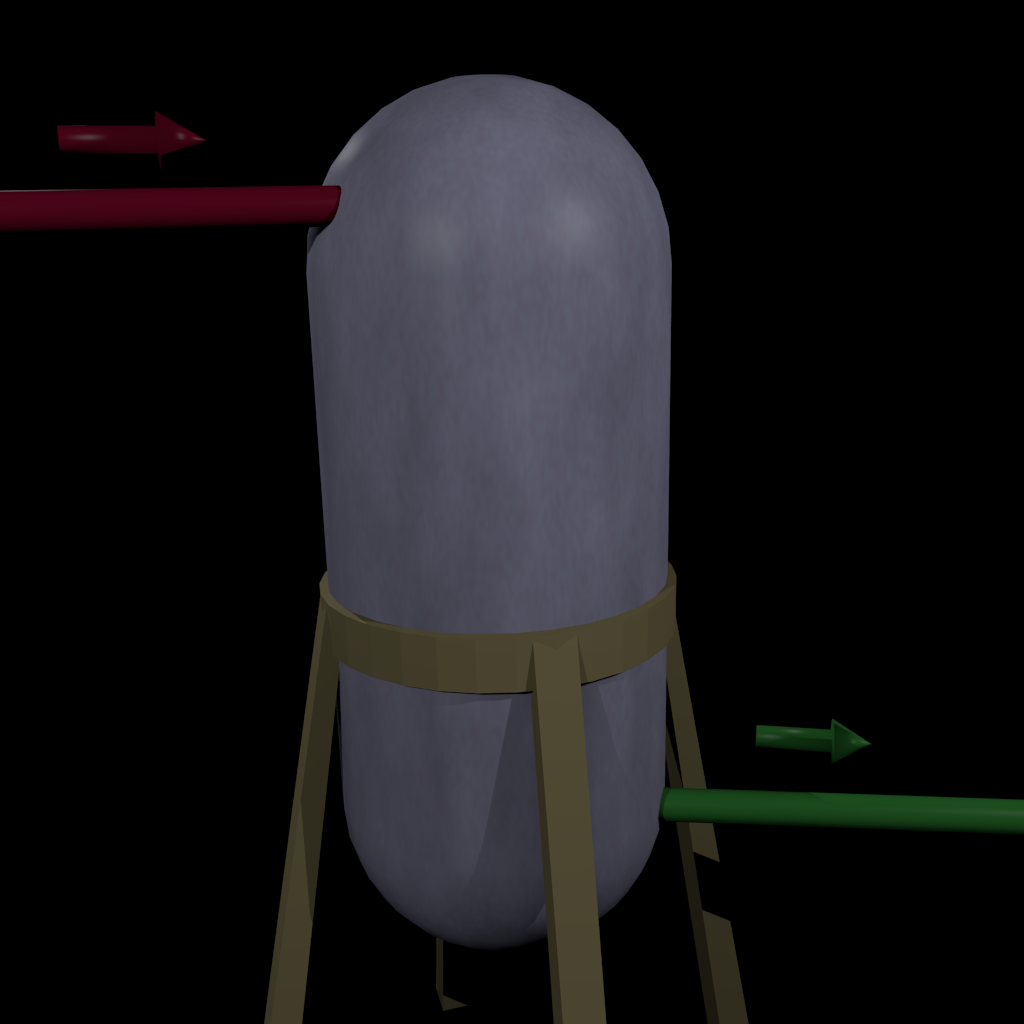
\includegraphics[width=8cm]{img/singleTank}}
  \only<2>{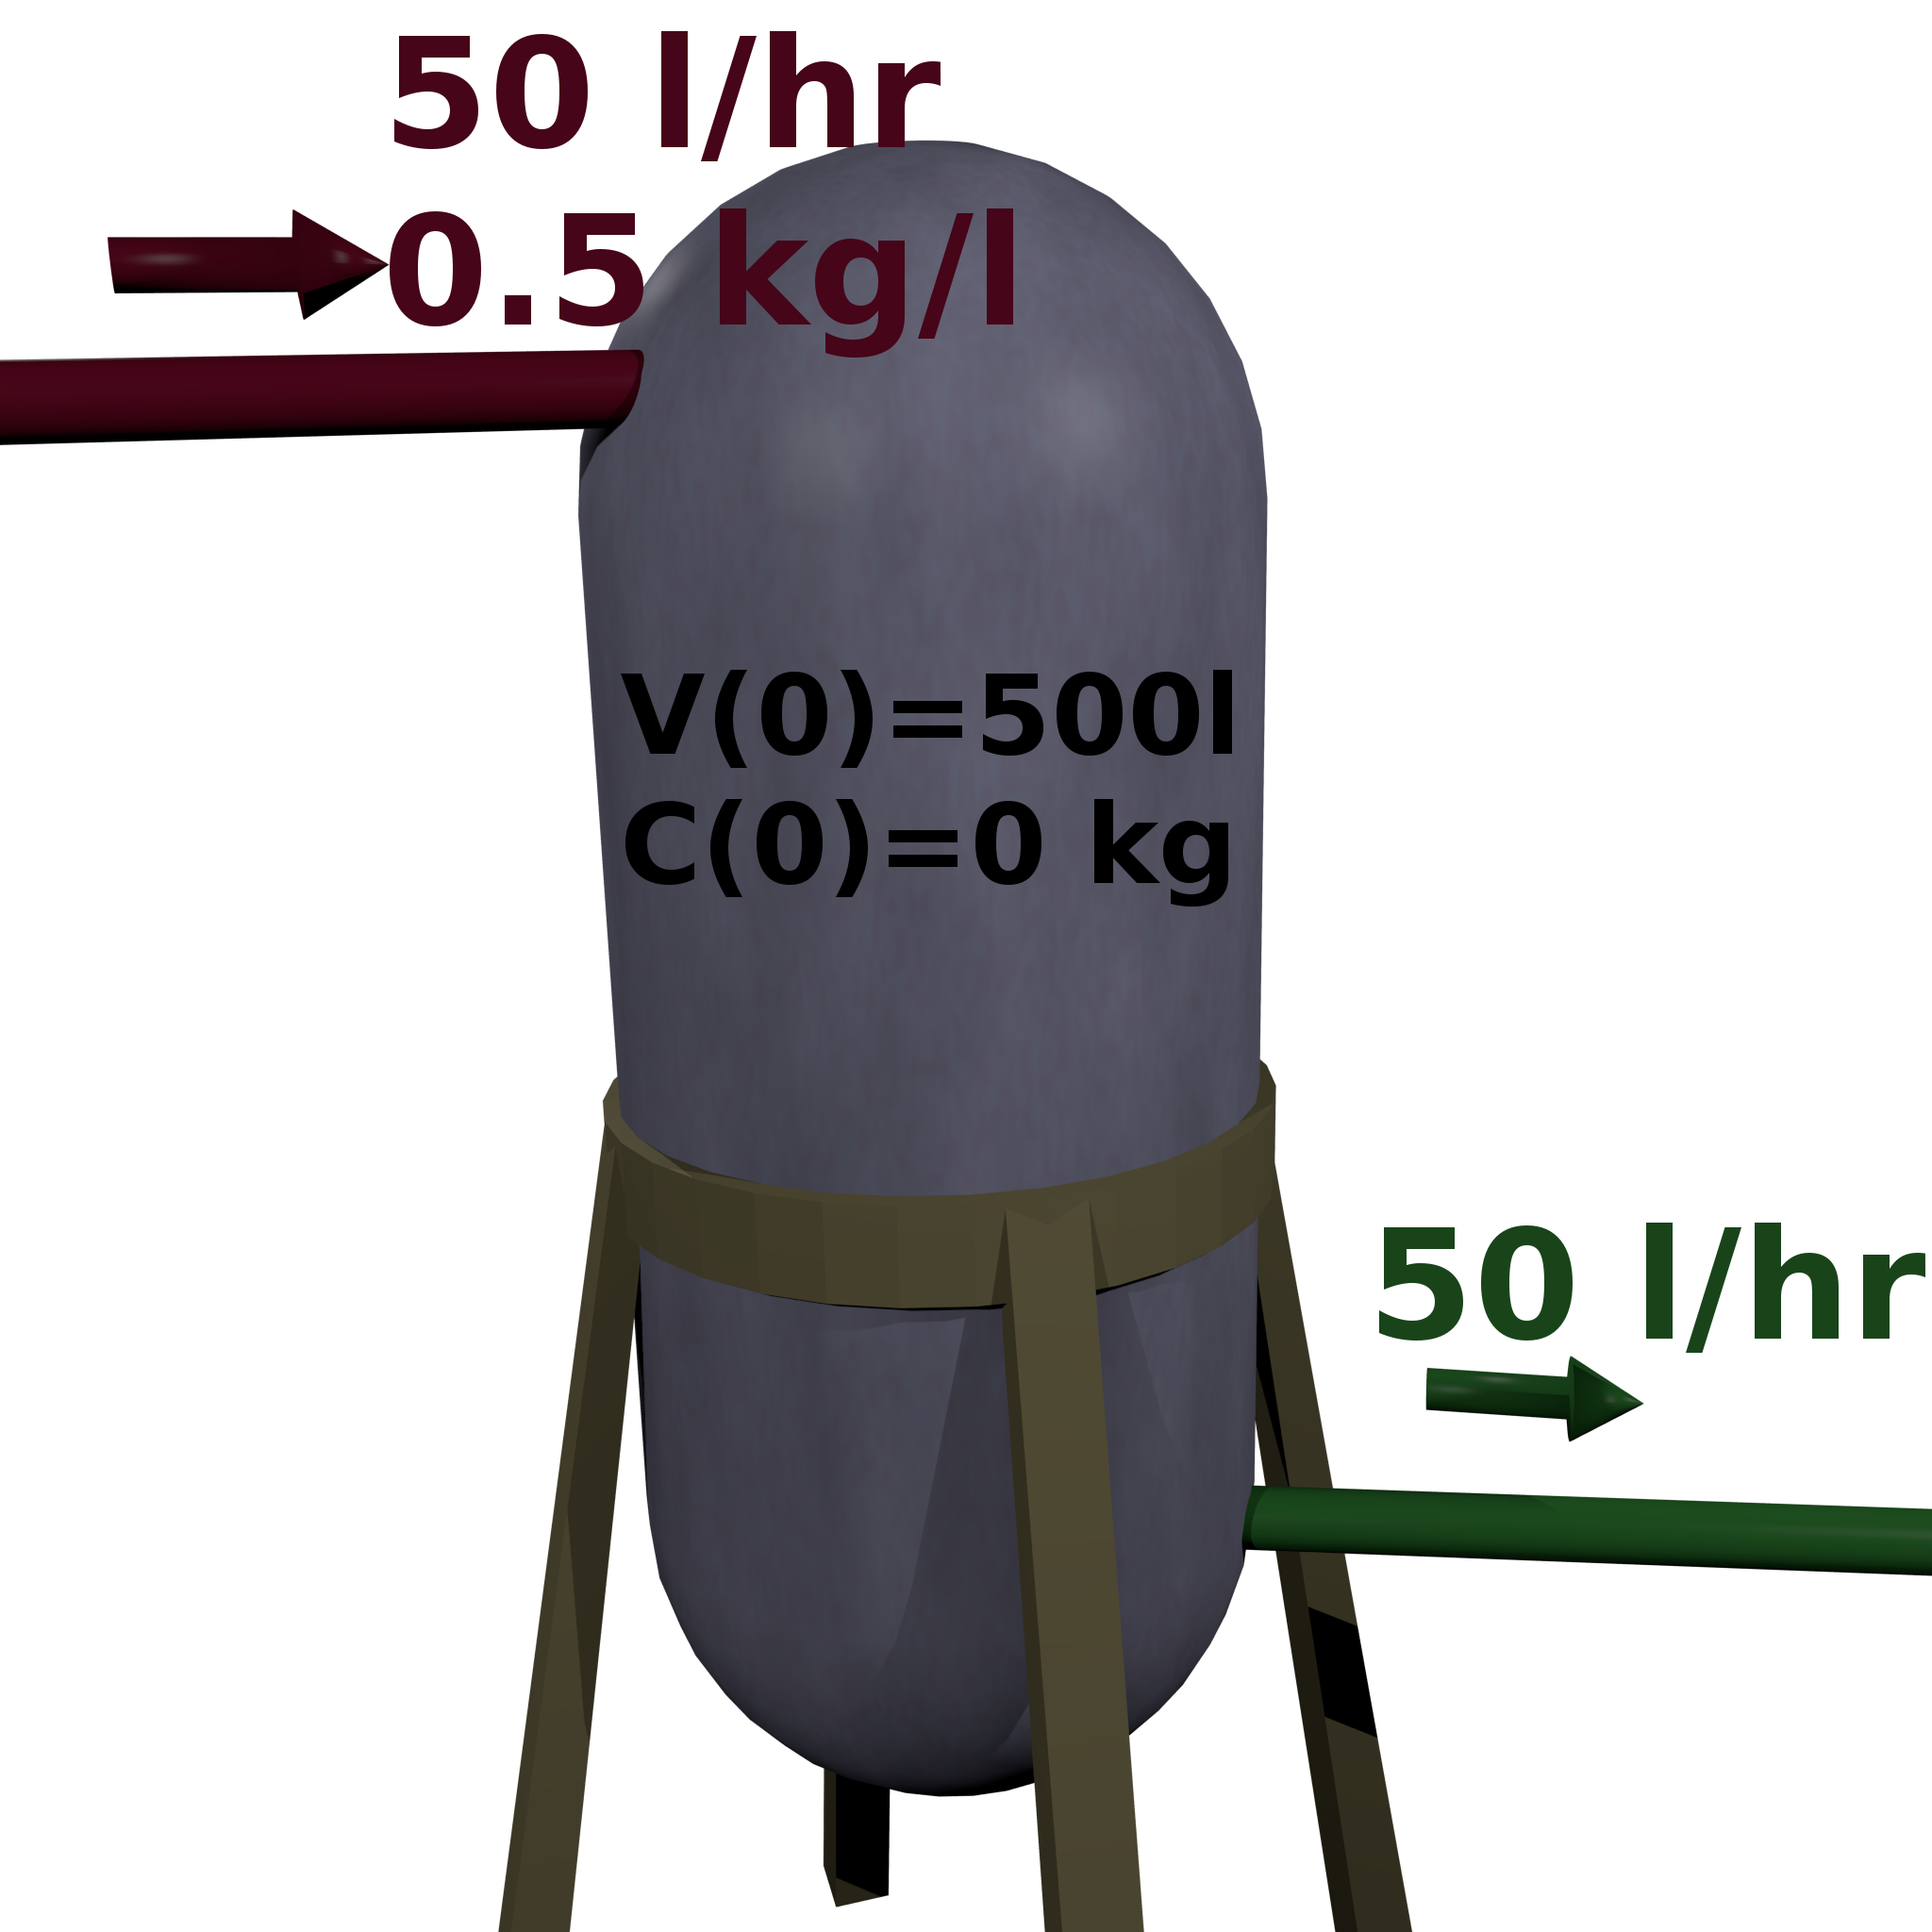
\includegraphics[width=8cm]{img/singleTankAnnotated}}
  
\end{frame}

\begin{frame}
  \frametitle{Conservation of Mass}

  Mass is conserved.

  \uncover<2->{Let $A(t)$ be the amount of ``stuff'' in the tank (kg).}

  \uncover<3->{

    \begin{eqnarray*}
      \Rightarrow ~ \frac{dA}{dt} & = & \mathrm{{\color{red}Rate ~ it ~ changes} ~
        (kg/hr)} \\
      & = & \mathrm{{\color{red}rate ~ in ~ - ~ rate ~ out}}.
    \end{eqnarray*}

  }

\end{frame}


\begin{frame}

  \begin{eqnarray*}
    \mathrm{rate~in~kg/hr} & = & \uncover<2->{.5 \frac{kg}{l} \cdot 50 \frac{l}{hr} \\
    & = & 25 \frac{kg}{hr}}
  \end{eqnarray*}

  \uncover<3->{

    \begin{eqnarray*}
      \mathrm{rate~out~kg/hr} & = & \uncover<4->{A(t)~kg \cdot
        \frac{1}{500~l} \cdot 50 \frac{l}{hr} \\
        & = & \frac{1}{10}A(t)}
    \end{eqnarray*}

  }

  \uncover<5->{

    \begin{eqnarray*}
      A'(t) & = & 25 - \frac{1}{10} A(t), \\
      A(0) & = & 0
    \end{eqnarray*}

  }

\end{frame}


\begin{frame}

  \begin{eqnarray*}
    \frac{1}{25 - \frac{1}{10}A} A' & = & 1, \\
    \int \frac{1}{25 - \frac{1}{10}A} A' ~ dt & = & \int 1 ~ dt, \\
    -10 \ln\lp25 - \frac{1}{10}A\rp & = & t + c \\
     \ln\lp25 - \frac{1}{10}A\rp & = & -\frac{t + c}{10} \\
     25 - \frac{1}{10} A & = & ke^{-t/10}, \\
     A & = & 250 - 10ke^{-t/10}, \\
     A(0) & = & 0 \\
     & = & 250-10k, \\
     k & = & 25, \\
     A(t) & = & 250-250e^{-t/10}
  \end{eqnarray*}

\end{frame}

\begin{frame}

  Concentration:
  \begin{eqnarray*}
    C(t) & = & A(t)/500 \\
    & = & \frac{1}{2} - \frac{1}{2} e^{-t/10}.
  \end{eqnarray*}

\end{frame}

\begin{frame}
  \frametitle{Example}

  {\color{red}A 2000 liter tank initially contains water with a solution of 0.2 kg
  per liter of salt.} {\color{blue} Brine is pumped in at a rate of 100 liters per
  hour with a concentration of 0.3 kg per liter.} {\color{purple}The well mixed
  solution is pumped out at a rate of 100 liters per hour.} Determine
  the amount of salt in the tank at any time.

  \vspace{1cm}
  Let $A(t)$ be the amount of salt in the tank at time $t$.
\end{frame}


\iftoggle{clicker}{%
\begin{frame}
  \frametitle{Clicker Quiz}
    
      \ifnum\value{clickerQuiz}=1{%

        What is the rate that salt flows into the tank?

       \vfill

       \begin{tabular}{l@{\hspace{3em}}l}
         A: & 10000 kg/hr. \\
         B: & 333.33 kg/hr. \\
         C: & 30 kg/hr. \\
         D: & 0.3 kg/hr. \\ 
       \end{tabular}

     }\fi

     \ifnum\value{clickerQuiz}=2{%

        What is the rate that salt flows into the tank?

       \vfill

       \begin{tabular}{l@{\hspace{3em}}l}
         A: & 10000 kg/hr. \\
         B: & 333.33 kg/hr. \\
         C: & 30 kg/hr. \\
         D: & 0.3 kg/hr. \\ 
       \end{tabular}


     }\fi

      \ifnum\value{clickerQuiz}=3{%
    What is the rate that salt flows into the tank?

       \vfill

       \begin{tabular}{l@{\hspace{3em}}l}
         A: & 10000 kg/hr. \\
         B: & 333.33 kg/hr. \\
         C: & 30 kg/hr. \\
         D: & 0.3 kg/hr. \\
       \end{tabular}

     }\fi

    \vfill
    \vfill
    \vfill

\end{frame}

}


\iftoggle{clicker}{%
\begin{frame}
  \frametitle{Clicker Quiz}
    
      \ifnum\value{clickerQuiz}=1{%

        What is the rate that salt flows out of the tank?

       \vfill

       \begin{tabular}{l@{\hspace{3em}}l}
         A: & A/20  kg/hr. \\
         B: & A/100 kg/hr. \\
         C: & 1/20  kg/hr. \\
         D: & 100   kg/hr. \\ 
       \end{tabular}

     }\fi

     \ifnum\value{clickerQuiz}=2{%

        What is the rate that salt flows out of the tank?

       \vfill

       \begin{tabular}{l@{\hspace{3em}}l}
         A: & A/20  kg/hr. \\
         B: & A/100 kg/hr. \\
         C: & 1/20  kg/hr. \\
         D: & 100   kg/hr. \\ 
       \end{tabular}

     }\fi

      \ifnum\value{clickerQuiz}=3{%
        What is the rate that salt flows out of the tank?

       \vfill

       \begin{tabular}{l@{\hspace{3em}}l}
         A: & A/20  kg/hr. \\
         B: & A/100 kg/hr. \\
         C: & 1/20  kg/hr. \\
         D: & 100   kg/hr. \\
       \end{tabular}


     }\fi

    \vfill
    \vfill
    \vfill

\end{frame}

}



\begin{frame}

  Let $A(t)$ be the amount of salt in the tank at time $t$.

  \begin{eqnarray*}
    A' & = & \mathrm{rate~in~} - \mathrm{~rate~out}.
  \end{eqnarray*}

  \begin{eqnarray*}
    \mathrm{rate~in} & = & 100 \frac{l}{hr} \cdot .3 \frac{kg}{l} \\
    & = & 30 \frac{kg}{hr}
  \end{eqnarray*}

  \begin{eqnarray*}
    \mathrm{rate~out} & = & A ~ kg \cdot \frac{1}{2000 l} \cdot 100 \frac{l}{hr} \\
    & = & \frac{1}{20} A
  \end{eqnarray*}

\end{frame}

\begin{frame}
   
  \begin{eqnarray*}
    A' & = & 30 - \frac{1}{20} A, \\
    A(0) & = & 2000 l \cdot .2 \frac{kg}{l} \\
    & = & 400 ~ kg
  \end{eqnarray*}

\end{frame}


\begin{frame}

  \begin{eqnarray*}
    A' + \frac{1}{20} A & = & 30 \\
    \uncover<2->{
      A' e^{t/20} + \frac{1}{20} e^{t/20} A & = & 30 e^{t/20} \\
      \frac{d}{dt} \lp A e^{t/20} \rp  & = & 30 e^{t/20} \\
      A e^{t/20}  & = & 600 e^{t/20} + C \\
      A  & = & 600 + C e^{-t/20} \\
      A(0) & = & 400 \\
      & = & 600 + C \\
      \Rightarrow C & = & -200 \\
      A(t) & = & 600-200 e^{-t/20}
    }
  \end{eqnarray*}

\end{frame}


\begin{frame}
  \frametitle{Example}

  {\color{red}A 500 liter tank is initially full and contains fresh water.} 
  {\color{blue}Brine with a concentration of 0.1 kg per liter is pumped into 
  the tank at a rate of 20 liters per hour.} {\color{purple}The well mixed 
  solution is pumped out at a rate of 30 liters per hour.}  
  What will the concentration be at the moment the tank is half full?

\end{frame}


\begin{frame}

  \begin{eqnarray*}
    A' & = & \mathrm{rate~in~} - \mathrm{~rate~out}
  \end{eqnarray*}

  \begin{eqnarray*}
    \mathrm{Rate~in} & = & .1 \frac{kg}{l} \cdot 20 \frac{l}{hr} \\
    & = & 2 \frac{kg}{l}
  \end{eqnarray*}

  \begin{eqnarray*}
    v(t) & = & 500-10t
  \end{eqnarray*}

  \begin{eqnarray*}
    \mathrm{rate~out} & = & A kg \cdot \frac{1}{500-10t ~ l} \cdot 30 \frac{l}{hr} \\
    & = & A \frac{30}{500-10t}
  \end{eqnarray*}

  \begin{eqnarray*}
    A' & = & 2 - A \frac{30}{500-10t}
  \end{eqnarray*}

\end{frame}


\begin{frame}

  \begin{eqnarray*}
    A' + A \frac{30}{500-10t} & = & 2 \\
    (500-10t)^{-3} A' + 30(500-10t)^{-4} A & = & 2 (500-10t)^{-3} \\
    \frac{d}{dt} \lp (500-10t)^{-3} A \rp & = & 2 (500-10t)^{-3} \\
    (500-10t)^{-3} A  & = & \int 2 (500-10t)^{-3} ~ dt  \\
    (500-10t)^{-3} A  & = & \frac{1}{10} (500-10t)^{-2} + C  \\
    A(0) & = & 0 \\
    & = & \frac{1}{10} 500^{-2} + C \\
    C & = & -\frac{1}{10\cdot500^{2}}
  \end{eqnarray*}

  \begin{eqnarray*}
    A(t) & = & \frac{1}{10} (500-10t) - \frac{1}{10\cdot500^{2}} (500-10t)^3
  \end{eqnarray*}

\end{frame}


\begin{frame}

  The tank is half full when the volume is 250l:
  \begin{eqnarray*}
    v(t) & = & 250 \\
    250 & = & 500-10t \\
    \Rightarrow t & = & 25.
  \end{eqnarray*}

  \begin{eqnarray*}
    A(25) & = & \frac{1}{10} (500-10\cdot 25) - \frac{1}{10\cdot500^{-2}} (500-10\cdot 25)^3 \\
    & \approx & 18.75 ~ kg
  \end{eqnarray*}

  \begin{eqnarray*}
    \mathrm{Concentration} & = & A(25)/250 \\
    & \approx & 0.075 kg/l
  \end{eqnarray*}

\end{frame}

\subsection{Newton's Law of Cooling}

\begin{frame}
  \frametitle{Newton's Law of Cooling}

  {\color{red}The rate of change of the temperature of an object is 
  proportional to the difference between the temperature of the 
  object and the temperature of the surroundings.}

  Let M be the ambient (the surroundings) temperature.  

  Let $T(t)$ be the temperature of the object at time $t$. 

  \begin{eqnarray*}
    T'(t) & = & k (M-T)
  \end{eqnarray*}


\end{frame}

\subsection{Examples of Newton's Law of Cooling}

\begin{frame}
  \frametitle{Example}

  {\color{red}A brick is pulled out of a furnace and is 350 degrees Celsius.} 
  {\color{blue}It is placed outside where the air temperature is 20 degrees Celsius.} 
  {\color{purple}After one hour the temperature of the brick is 280
    degrees Celsius.}  
  What will the temperature of the brick be after 6 hours from when it
  was first pulled out of the furnace?

  \uncover<2->{
    
    \begin{eqnarray*}
      T' & = & k(M-T) \\
      T(0) & = & 350 \\
      M & = & 20 \\
      T(1) & = & 280 \\
      T(6) & = & ??
    \end{eqnarray*}

  }

\end{frame}


\begin{frame}

  \begin{eqnarray*}
    T' & = & k (20-T) \\
    \frac{T'}{20-T} & = & k \\
    -\ln(T-20) & = & kt + C,  \text{since} T > 20\\
    T & = & 20 + A e^{-kt}
  \end{eqnarray*}

  \begin{eqnarray*}
    T(0) & = & 350 \\
    & = & 20 + A \\
    A & = & 330, \\
    T(t) & = & 20 + 330 e^{-kt}
  \end{eqnarray*}

\end{frame}


\begin{frame}

  \begin{eqnarray*}
    T(1) & = & 280 \\
    & = & 20 + 330 e^{-k} \\
    k & = & -\ln\lp\frac{26}{33}\rp \\
    T(t) & = & 20 + 330 e^{t\ln\lp\frac{26}{33}\rp}
  \end{eqnarray*}

  \begin{eqnarray*}
    T(6) & = & 20 + 330 e^{6\ln\lp\frac{26}{33}\rp} \\
    & \approx & 98.9 ~C
  \end{eqnarray*}

\end{frame}


\begin{frame}
  \frametitle{Example}

  A cup of coffee is found. {\color{red}The temperature when it is found is 70
  degrees Celsius.} {\color{blue}Thirty minutes later its temperature is 65 degrees
  Celsius.} {\color{purple}The temperature in the room is 18 degrees Celsius.} 
  {\color{orange}When the coffee was poured the temperature was 85 degrees Celsius.} 
  When was the coffee poured?

  \uncover<2->{
    
    \begin{eqnarray*}
      t_0 & = & \mathrm{time~when~the~coffee~was~found.} \\
      M & = & 18 \\
      T(0) & = & 85   \\
      T(t_0) & = & 70 \\
      T(t_0+30) & = & 65.
    \end{eqnarray*}

  }

\end{frame}


\begin{frame}

  \begin{eqnarray*}
    T' & = & k(18-T) \\
    \frac{T'}{18-T} & = & k \\
    -\ln(T-18) & = & kt + C \\
    T & = & 18 + A e^{-kt} 
  \end{eqnarray*}

\end{frame}

\begin{frame}

  At time $t_0$:
  \begin{eqnarray*}
    T(t_0) & = & 70 \\
    & = & 18 + Ae^{-kt_0} \\
    \Rightarrow Ae^{-kt_0} & = & 52
  \end{eqnarray*}

  At time $t_0+30$:
  \begin{eqnarray*}
    A(t_0+30) & = & 65 \\
    & = & 18 + A e^{-kt_0-30k} \\
    & = & 18 + A e^{-kt_0} e^{-30k} \\
    & = & 18 + 52 e^{30k} \\
    \Rightarrow k & = & -\frac{1}{30} \ln\lp\frac{47}{52}\rp.
  \end{eqnarray*}

\end{frame}


\begin{frame}

  \begin{eqnarray*}
    T(0) & = & 85 \\
    & = & 18 + A e^{0} \\
    \Rightarrow A & = & 67
  \end{eqnarray*}

  \begin{eqnarray*}
    T(t)  & = & 18 + 67 e^{\frac{t}{30} \ln\lp\frac{47}{52}\rp} \\
    T(t_0)& = & 70 \\
    & = & 18 + 67 e^{\frac{t_0}{30} \ln\lp\frac{47}{52}\rp} \\
    \Rightarrow t_0 & = & \frac{30\ln\lp\frac{52}{67}\rp}{\ln\lp\frac{47}{52}\rp}.
  \end{eqnarray*}

\end{frame}



% LocalWords:  Clarkson pausesection hideothersubsections

\part{Autonomous-ODEs}
\lecture{Autonomous ODEs}{Autonomous-ODEs}
\section{Autonomous ODEs}

\title{Ordinary Differential Equations}
\subtitle{Math 232 - Week 3, Day 2}
\date{12 Sep 2012}

\begin{frame}
  \titlepage
\end{frame}

\begin{frame}
  \frametitle{Outline}
  \tableofcontents[pausesection,hideothersubsections]

  Section 2.5 in book.
\end{frame}


\subsection{Solutions to DEs}


\begin{frame}
  \frametitle{What is a solution to a DE?}

  What is the solution to the DE

  \begin{eqnarray*}
    y' & = & t^2 + y^2?
  \end{eqnarray*}

  \uncover<2->{I do not know!}


\end{frame}


\begin{frame}
  \frametitle{Slope Field}

  Look at the slope field:
  \begin{eqnarray*}
    y' & = & t^2 + y^2?
  \end{eqnarray*}

  % TODO - make this image higher resolution!
  \only<1>{\includegraphics[height=5cm]{img/week3-D3SlopeExample}}
  \only<2->{\includegraphics[height=5cm]{img/week3-D3SlopeExampleSolutions}}

  Look at equilibria, stability, and look for straight line solutions.

\end{frame}


\iftoggle{clicker}{%
\begin{frame}
  \frametitle{Clicker Quiz}
    
      \ifnum\value{clickerQuiz}=1{%

        Look at the slope field:
        \begin{eqnarray*}
          y' & = & -t - y^2?
        \end{eqnarray*}

        \begin{columns}
          \column{.6\textwidth} 

          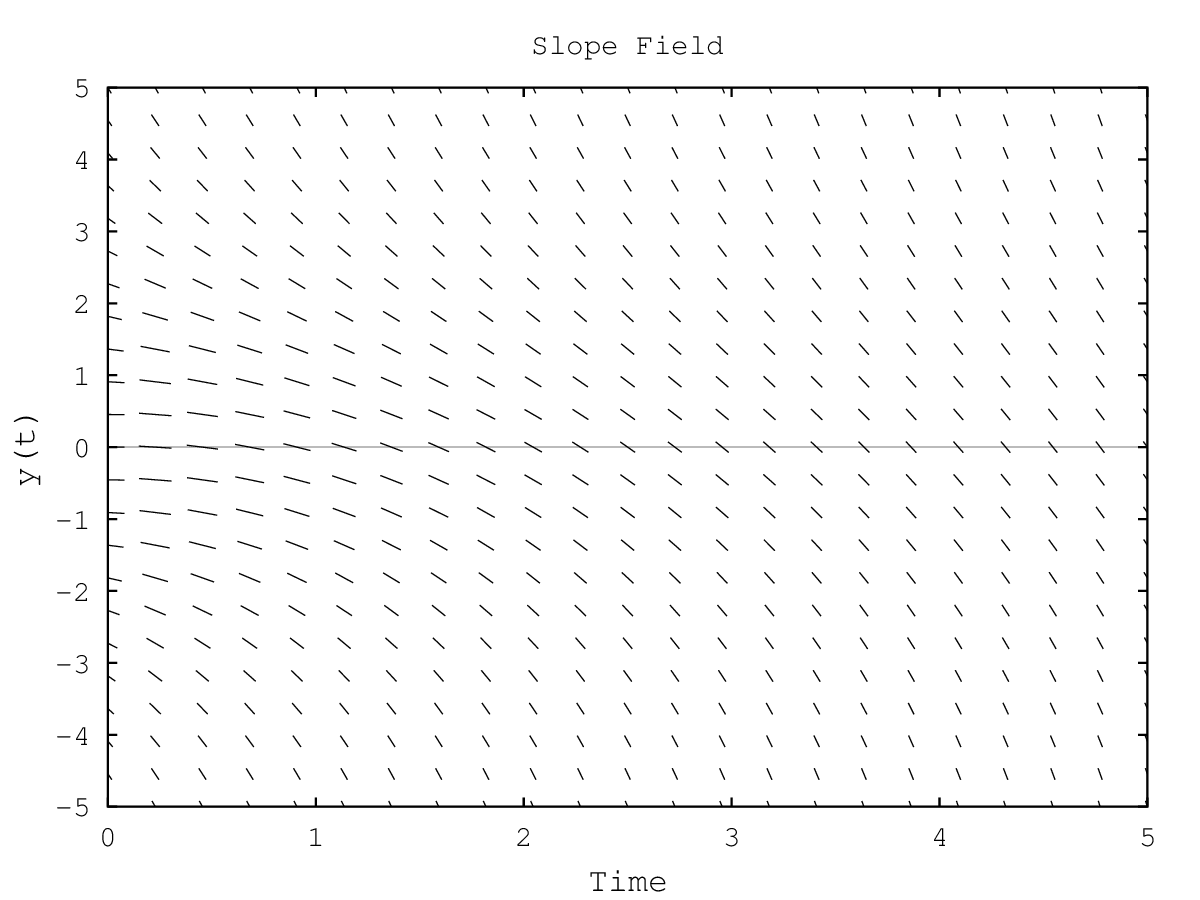
\includegraphics[height=5cm]{img/stabilityClicker1}

          \column{.4\textwidth}
          True or False: The solution to this differential equation is stable.

          \begin{tabular}{l@{\hspace{3em}}l}
            A: & True. \\
            B: & False. \\
            C: & Who knows? \\
            D: & Truth is subjective. \\ 
          \end{tabular}

        \end{columns}

     }\fi

     \ifnum\value{clickerQuiz}=2{%

        Look at the slope field:
        \begin{eqnarray*}
          y' & = & \frac{3}{2}-y?
        \end{eqnarray*}


        \begin{columns}
          \column{.6\textwidth} 

          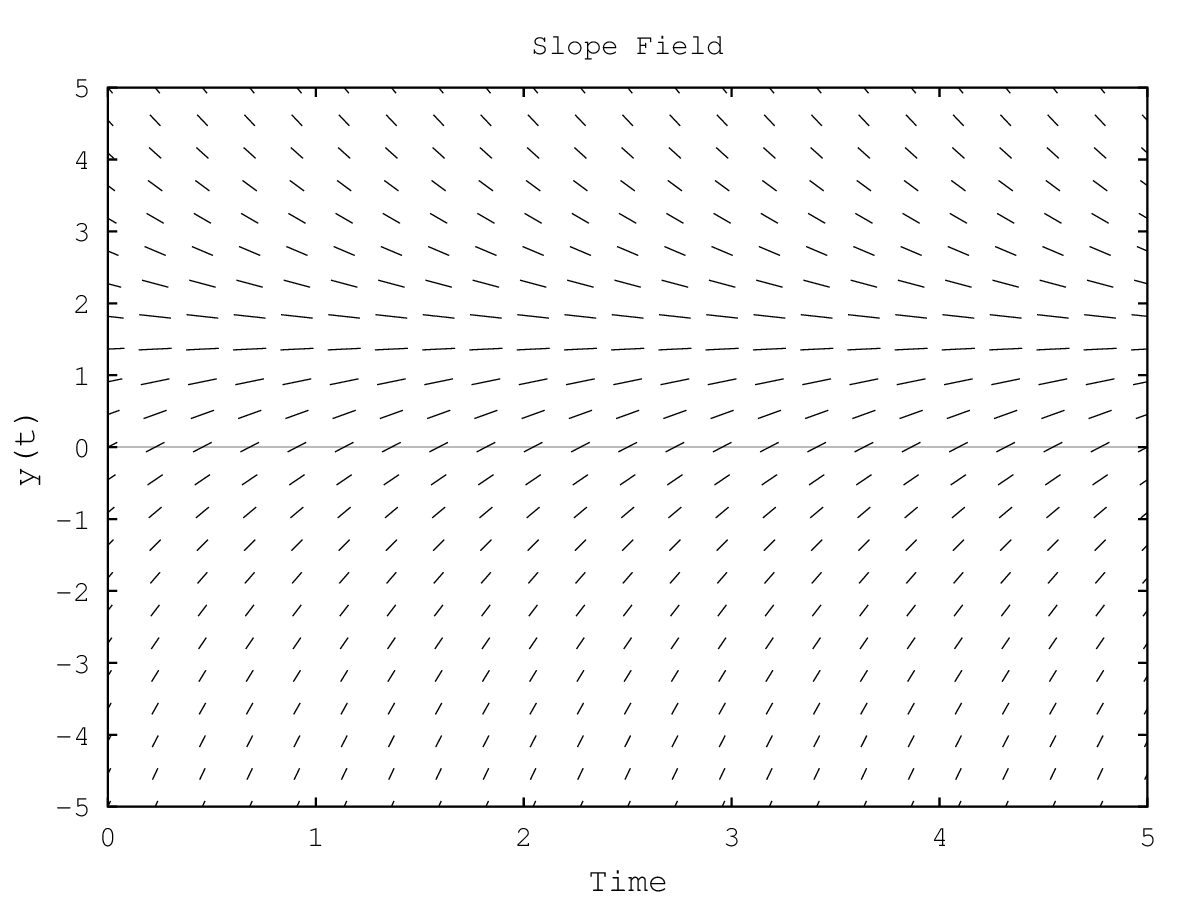
\includegraphics[height=5cm]{img/stabilityClicker2}

          \column{.4\textwidth}
          True or False: The solution to this differential equation is stable.

          \begin{tabular}{l@{\hspace{3em}}l}
            A: & True. \\
            B: & False. \\
            C: & Who knows? \\
            D: & Truth is subjective. \\ 
          \end{tabular}

        \end{columns}

     }\fi

      \ifnum\value{clickerQuiz}=3{%
      Look at the slope field:
        \begin{eqnarray*}
          x' & = & x^2-4?
        \end{eqnarray*}


        \begin{columns}
          \column{.6\textwidth}

          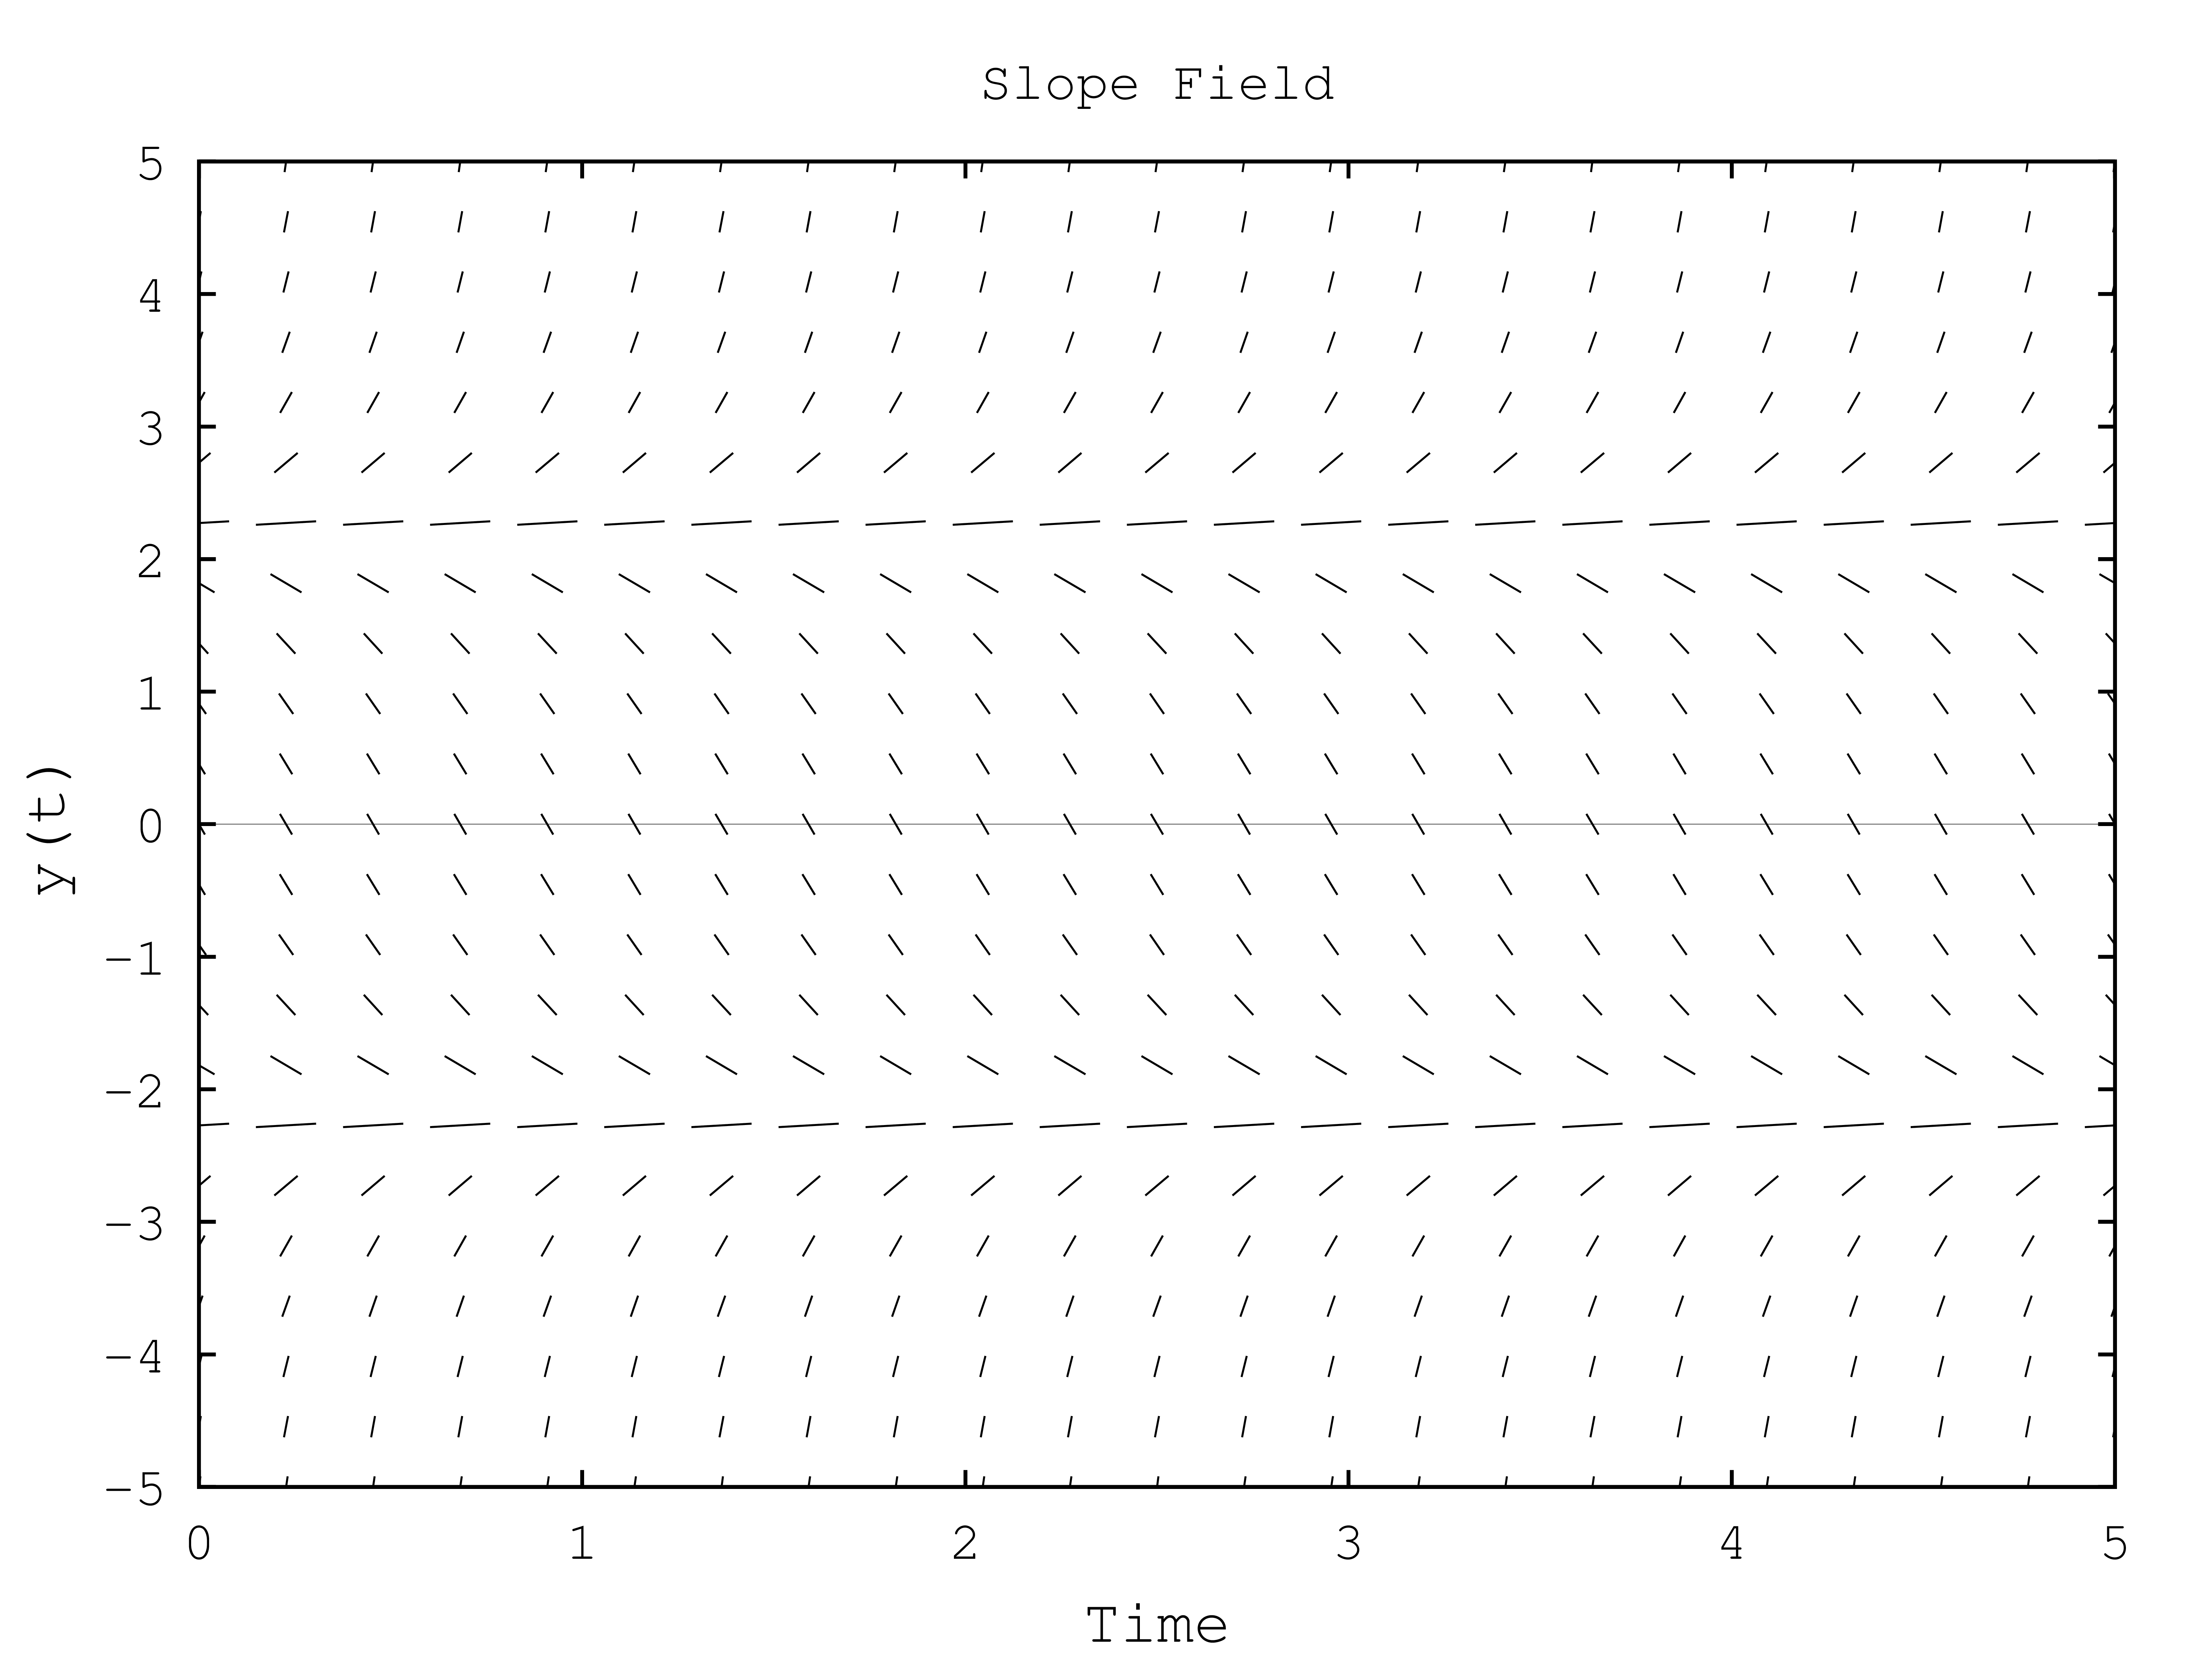
\includegraphics[height=5cm]{img/slopefield2}

          \column{.4\textwidth}
          True or False: The solution to this differential equation is stable.

          \begin{tabular}{l@{\hspace{1em}}l}
            A: & True. \\
            B: & False. \\
            C: & Who knows? \\
            D: & Truth is subjective. \\
          \end{tabular}

        \end{columns}

     }\fi

    \vfill
    \vfill
    \vfill

\end{frame}

}


\subsection{Autonomous DEs}

\begin{frame}
  \frametitle{Autonomous DEs}

  A differential equation is \textit{autonomous} if it can be
  expressed in the form
  \begin{eqnarray*}
    y' & = & f(y).
  \end{eqnarray*}

  i.e. the DE does not have a time term explicitly given in the
  equation.


\end{frame}


\begin{frame}
  \frametitle{The slope only depends on y!}

  \vspace*{-3em}
  \begin{eqnarray*}
    y' & = & f(y).
  \end{eqnarray*}

  If the slope at $y=1$ and $t=1$ is $\half$, then it will be the same
  slope for all points where $y=1$. 

  \vfill
  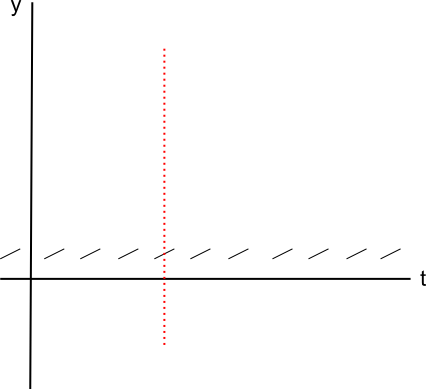
\includegraphics[width=5cm]{img/autonomousEqnSlopeField}
  \vfill

  We just need to find the slope for each value of $y$ and not worry
  about $t$.

\end{frame}

\begin{frame}
  \frametitle{The Phase Line}

  The phase line for a differential equation is a vertical line that
  indicates whether the slope is positive, negative, or zero for
  different values of $y$.
\end{frame}

\begin{frame}
  \frametitle{Example}
  \begin{eqnarray*}
    y' & = & 2y(3-y), \\
    \Rightarrow f(y) & = & 2y(3-y)
  \end{eqnarray*}


  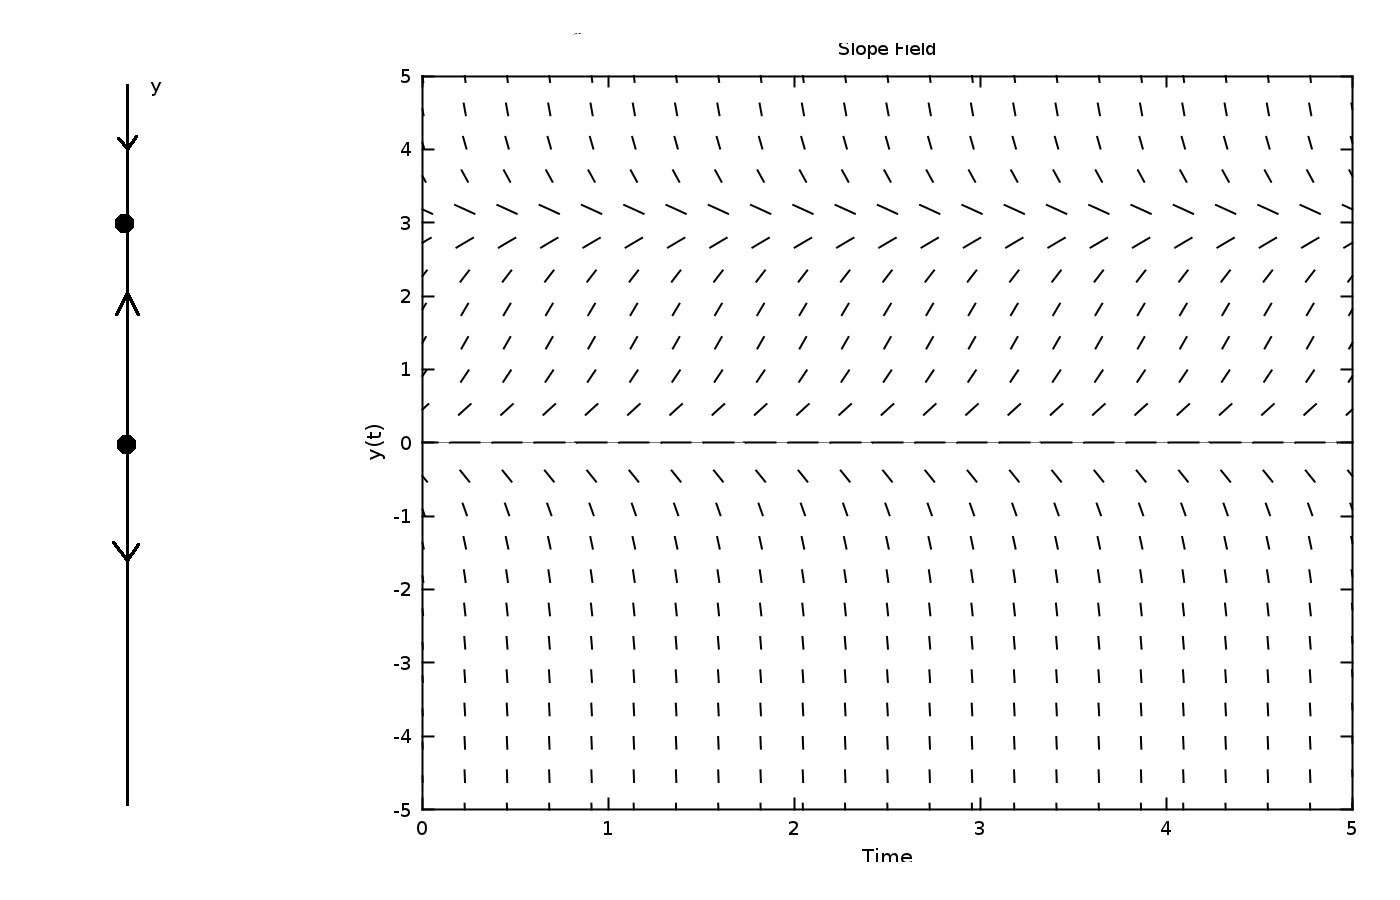
\includegraphics[height=6cm]{img/week3PhaseLineExample1}

\end{frame}


\begin{frame}
  \frametitle{Examples}
  
  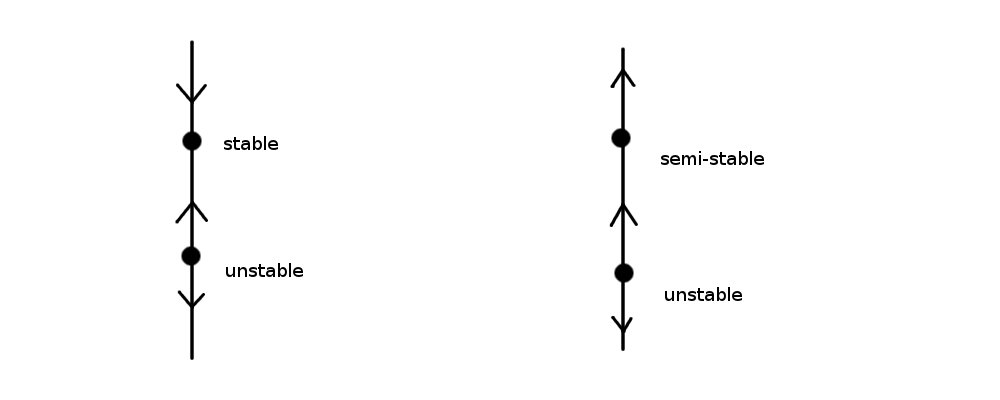
\includegraphics[height=6cm]{img/week3PhaseLine}

\end{frame}

\begin{frame}
  \frametitle{Examples}


  \begin{eqnarray*}
    y' & = & y(2-y)(4-y), \\
    \Rightarrow f(y) & = & y(2-y)(4-y)
  \end{eqnarray*}

  \begin{eqnarray*}
    y' & = & y(2-y^2), \\
    \Rightarrow f(y) & = & y(2-y^2)
  \end{eqnarray*}

  (phase lines drawn on board)

\end{frame}

\iftoggle{clicker}{%
\begin{frame}
  \frametitle{Clicker Quiz}
    
      \ifnum\value{clickerQuiz}=1{%

        Which phase line is the correct phase line for the
        differential equation
        \begin{eqnarray*}
          y ' & = & y^3-y^2
        \end{eqnarray*}

          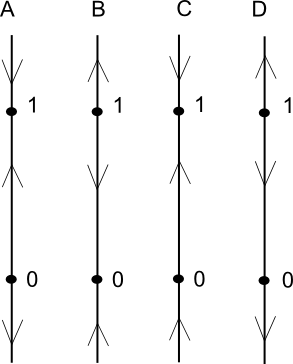
\includegraphics[height=5cm]{img/phaseLinesClickerSect1}

     }\fi

     \ifnum\value{clickerQuiz}=2{%


        Which phase line is the correct phase line for the
        differential equation
        \begin{eqnarray*}
          y ' & = & y^2 + 3y - 4
        \end{eqnarray*}

        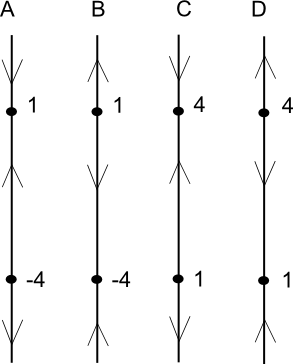
\includegraphics[height=5cm]{img/phaseLinesClickerSect2}


     }\fi

      \ifnum\value{clickerQuiz}=3{%
       Which phase line is the correct phase line for the
        differential equation
        \begin{eqnarray*}
          y ' & = & y^3-y^2
        \end{eqnarray*}

          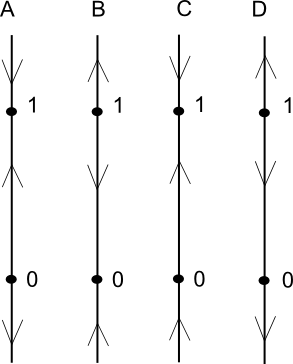
\includegraphics[height=5cm]{img/phaseLinesClickerSect1}
     }\fi

    \vfill
    \vfill
    \vfill

\end{frame}

}



\subsection{Logistic Growth}

\begin{frame}
  \frametitle{Logistic Growth}

  \vspace*{-4em}
  \begin{eqnarray*}
    y' & = & ky,
  \end{eqnarray*}
  
  If $y$ is ``small'' $k$ should be positive.

  If $y$ is ``big'' $k$ should be negative.

  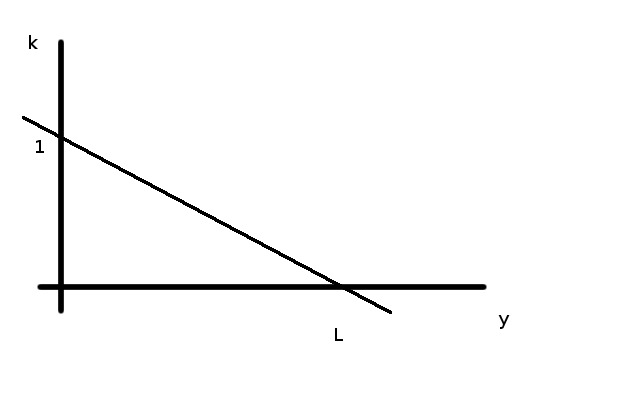
\includegraphics[height=4cm]{img/week3GrowthRate}

  Let 
  \begin{eqnarray*}
    k & = & r \lp 1 - \frac{y}{L} \rp
  \end{eqnarray*}


\end{frame}


\begin{frame}
  \frametitle{Logistic Equation}

  \begin{eqnarray*}
    y' & = & r \lp 1 - \frac{y}{L} \rp y
  \end{eqnarray*}

  Stationary points: $y=0$ and $y=L$. 

  ($L$ is called the ``carrying capacity'')

  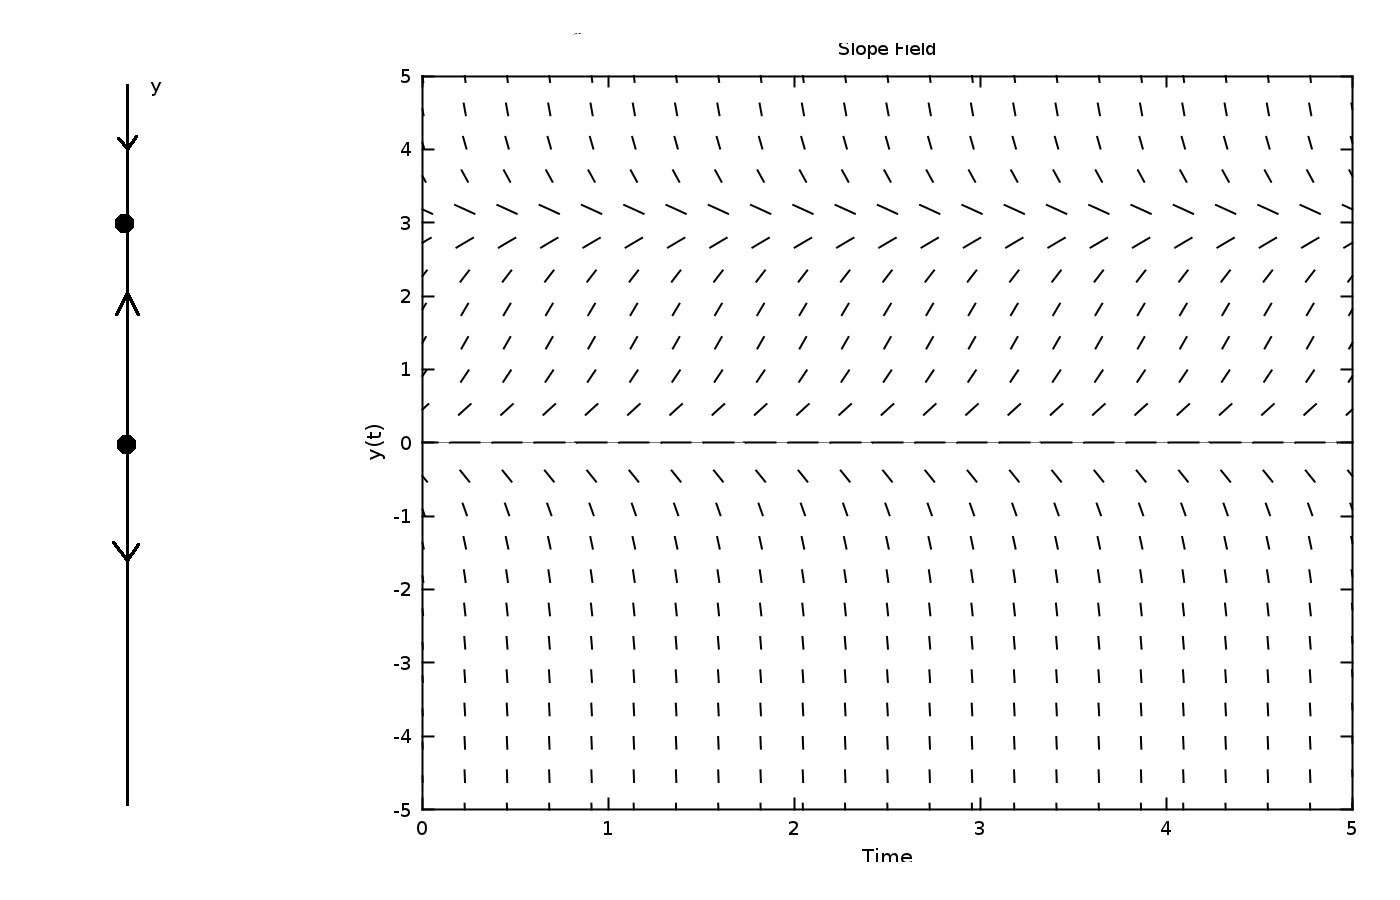
\includegraphics[height=6cm]{img/week3PhaseLineExample1}

\end{frame}


\begin{frame}
  \frametitle{Analytic Solution}

  \begin{eqnarray*}
    y' & = & r \lp 1 - \frac{y}{L} \rp y, \\
    \uncover<2->{
      \frac{y'}{\lp 1 - \frac{y}{L} \rp y} & = & r \\
      \int \frac{y'}{\lp 1 - \frac{y}{L} \rp y} ~ dt & = & \int r ~ dt       
    }
  \end{eqnarray*}

\end{frame}


\begin{frame}


  \begin{eqnarray*}
    \frac{1}{\lp 1 - \frac{y}{L} \rp y} & = & \frac{a}{1 - \frac{y}{L}} + \frac{b}{y} \\
    \Rightarrow 1 & = & a y + b \lp 1 - \frac{y}{L} \rp \\
    b & = & 1, \\
    a & = & \frac{1}{L}
  \end{eqnarray*}

    
\end{frame}

  \begin{frame}

  \begin{eqnarray*}
      \int \frac{1}{\lp 1 - \frac{y}{L} \rp y} ~ dy & = & \int r ~ dt \\
      \int \frac{1}{L} \cdot \frac{1}{1 - \frac{y}{L}} + \frac{1}{y} ~ dy & = & \int r ~ dt \\
      -\ln\lp 1 - \frac{y}{L}\rp + \ln(y) & = & rt + C \\
      \ln\lp\frac{y}{1 - \frac{y}{L}}\rp & = & rt + C \\
      \frac{y}{1 - \frac{y}{L}} & = & k e^{rt} \\
      \Rightarrow y & = & \frac{k e^{rt}}{1 + \frac{1}{L} k e^{rt}}  
  \end{eqnarray*}


  From the initial condition,
  \begin{eqnarray*}
    y(0) & = & y_0, \\
    k & = & \frac{y_0}{1 - \frac{y_0}{L}}
  \end{eqnarray*}
  

\end{frame}



% LocalWords:  Clarkson pausesection hideothersubsections




% %%%%%%%%%%%%%%%%%%%%%%%%%%%%%%%%%%%%%%%%%%%%%%%%%%%%%%%%%%%%
% Start of complex numbers and linear algebra

\part{Complex-Numbers-I}
\lecture{Complex Numbers I}{Complex-Numbers-I}
\section{Complex Numbers}

\title{Ordinary Differential Equations}
\subtitle{Math 232 - Week 4, Day 1}
\date{16 September 2013}

\begin{frame}
  \titlepage
\end{frame}

\begin{frame}
  \frametitle{Outline}
  \tableofcontents[currentsection]
\end{frame}


\subsection{The Letter i}


\begin{frame}
  \frametitle{The Letter i}

  Definition:
  \begin{eqnarray*}
    i & = & \sqrt{-1}
  \end{eqnarray*}

  Which means....
  \begin{eqnarray*}
    i^2 & = & -1
  \end{eqnarray*}

\end{frame}


\begin{frame}
  \frametitle{Complex Numbers}

  \begin{definition}
    A \redText{complex number} is a number that can be expressed as
    \begin{eqnarray*}
      a + bi,
    \end{eqnarray*}
    where $a$ and $b$ are real numbers.
  \end{definition}


\end{frame}



\begin{frame}
  \frametitle{Example}

  \begin{eqnarray*}
    z_1 & = & 3 + 2i \\
    z_2 & = & 5 - 7i
  \end{eqnarray*}

\end{frame}

\subsection{Operations With Complex Numbers}

\begin{frame}
  \frametitle{Addition}

  \begin{eqnarray*}
    (3+2i) + (5-7i) & = &
    \uncover<2->{%
      (3+5) + (2-7)i \\
      & = & 8 - 5i\\
    }
    ~ \\
    (4-2i) + (6-3i) & = &
    \uncover<3->{%
      (4+6) + (-2-3)i \\
      & = & 10 - 5i
    }
  \end{eqnarray*}

\end{frame}

\begin{frame}
  \frametitle{Multiplication}

  \begin{eqnarray*}
    (3+2i)(5-7i) & = &
    \uncover<2->{%
      15 + 10i - 21i - 14 i^2 \\
      & = & 15 - 11i + 14 \\
      & = & 29 - 11 i
    }
  \end{eqnarray*}

  \begin{eqnarray*}
    (4-2i)(6+3i) & = &
    \uncover<3->{%
      24 - 12i + 12 i - 6i^2 \\
      & = & 24 + 6 \\
      & = & 30
    }
  \end{eqnarray*}

\end{frame}


\subsection{Complex Conjugate}

\begin{frame}
  \frametitle{The Complex Conjugate}

  \begin{definition}
    The \redText{complex conjugate} of $z$, denoted $\bar{z}$, is
    found by reversing the sign of the imaginary part.
  \end{definition}

<<<<<<< HEAD

=======
  
>>>>>>> 5aff3be819a5e3e45e415346143eb989565538b4
  Example:
  For each of the numbers given below:
  \begin{eqnarray*}
    z_1 & = & 3 + 2i, \\
    z_2 & = & 5 - 6i,
  \end{eqnarray*}
  the complex conjugates are the following:
  \begin{eqnarray*}
    \bar{z_1} & = & 3 - 2i, \\
    \bar{z_2} & = & 5 + 6i.
  \end{eqnarray*}


\end{frame}

\begin{frame}
  \frametitle{Special Property of the Complex Conjugate}

  \begin{eqnarray*}
    z\cdot\bar{z} & = & (a+bi)(a-bi) \\
    & = & a^2 +abi - abi - b^2 i^2 \\
    & = & a^2 + b^2
  \end{eqnarray*}

\end{frame}



\begin{frame}
  \frametitle{So What?}

  \begin{eqnarray*}
    \frac{5-3i}{2+3i} & = &
    \uncover<2->{%
      \frac{(5-3i)(2-3i)}{(2+3i)(2-3i)} \\
      & = & \frac{10-6i-15i+9i^2}{4+6i-6i-9i^2} \\
      & = & \frac{1-21i}{13} \\
      & = & \frac{1}{13} - \frac{21}{13} i
    }
  \end{eqnarray*}

\end{frame}

\begin{frame}
  \frametitle{Example}

  \begin{eqnarray*}
    \frac{2+3i}{5-3i} & = &
    \uncover<2->{%
      \frac{(2+3i)(5+3i)}{(5-3i)(5+3i)} \\
      & = & \frac{10+15i+6i+9i^2}{25-15i+15i-9i^2} \\
      & = & \frac{1+21i}{34} \\
      & = & \frac{1}{34} + \frac{21}{34}i
    }
  \end{eqnarray*}

\end{frame}

\subsection{Graphical View of Complex Numbers}

\begin{frame}
  \frametitle{Graphical View of Complex Numbers}

  \only<1>{\centerline{\includegraphics[width=4cm]{img/complexPlane}}}
  \only<2>{\centerline{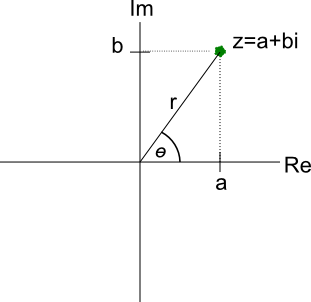
\includegraphics[width=4cm]{img/complexPlanePolar}}}

  \begin{eqnarray*}
    a & = & r\cos(\theta) \\
    b & = & r\sin(\theta) \\
    r & = & \sqrt{a^2+b^2} \\
    \tan(\theta) & = & \frac{b}{a}
  \end{eqnarray*}
  (Be careful about the arctangent. Your calculator lies!)

\end{frame}


\begin{frame}
  \frametitle{Example}

  \begin{eqnarray*}
<<<<<<< HEAD
    z & = & 2 + 2i
=======
    z & = &  2 + 2i
>>>>>>> 5aff3be819a5e3e45e415346143eb989565538b4
  \end{eqnarray*}

  \uncover<2->
  {%

    \begin{eqnarray*}
      r & = & \sqrt{2^2+2^2}, \\
        & = & 2\sqrt{2}, \\
      \tan(\theta) & = & \frac{2}{2}, \\
      \theta & = & \frac{\pi}{4}.
    \end{eqnarray*}

  }

\end{frame}


\iftoggle{clicker}{%
\begin{frame}
  \frametitle{Clicker Quiz}

      \ifnum\value{clickerQuiz}=1{%

        Determine the radius and angle for the following complex number:
          \begin{eqnarray*}
            z & = & -2 + 2i
          \end{eqnarray*}


          \begin{tabular}{l@{\hspace{3em}}l@{\hspace{1em}}l}
            A: & $r=2$, & $\theta= -\pi/4$ \\
            B: & $r=2$, & $\theta= 3\pi/4$ \\
            C: & $r=2\sqrt{2}$, & $\theta= -\pi/4$ \\
            D: & $r=2\sqrt{2}$, & $\theta= 3\pi/4$ \\
          \end{tabular}

     }\fi

     \ifnum\value{clickerQuiz}=2{%

        Determine the radius and angle for the following complex number:
          \begin{eqnarray*}
            z & = & -2 -2i
          \end{eqnarray*}


          \begin{tabular}{l@{\hspace{3em}}l@{\hspace{1em}}l}
            A: & $r=2$, & $\theta= -\pi/4$ \\
            B: & $r=2$, & $\theta= 5\pi/4$ \\
            C: & $r=2\sqrt{2}$, & $\theta= -\pi/4$ \\
            D: & $r=2\sqrt{2}$, & $\theta= 5\pi/4$ \\
          \end{tabular}

     }\fi

      \ifnum\value{clickerQuiz}=3{%

        Determine the radius and angle for the following complex number:
          \begin{eqnarray*}
            z & = & -2 + 2i
          \end{eqnarray*}


          \begin{tabular}{l@{\hspace{3em}}l@{\hspace{1em}}l}
<<<<<<< HEAD
            A: & $r=2$, & $\theta= -\pi/4$ \\
            B: & $r=2$, & $\theta= 3\pi/4$ \\
            C: & $r=2\sqrt{2}$, & $\theta= -\pi/4$ \\
            D: & $r=2\sqrt{2}$, & $\theta= 3\pi/4$ \\
=======
            A: &  $r=2$, & $\theta= -\pi/4$ \\
            B: &  $r=2$, & $\theta= 3\pi/4$ \\
            C: &  $r=2\sqrt{2}$, & $\theta= -\pi/4$ \\
            D: &  $r=2\sqrt{2}$, & $\theta= 3\pi/4$ \\ 
>>>>>>> 5aff3be819a5e3e45e415346143eb989565538b4
          \end{tabular}


     }\fi

    \vfill
    \vfill
    \vfill

\end{frame}

}



\subsection{Euler's Formula}

\begin{frame}
  \frametitle{A Differential Equation}

  \textbf{Note: \redText{$i$ is a constant.}}
  \begin{eqnarray*}
    \Rightarrow \frac{d}{dt} e^{it} & = & i e^{it}.
  \end{eqnarray*}

  The function
  \begin{eqnarray*}
    y(t) & = & e^{it}
  \end{eqnarray*}
  is \textbf{\redText{the}} solution to the differential equation
  \begin{eqnarray*}
    y' & = & iy, \\
    y(0) & = & 1.
  \end{eqnarray*}

\end{frame}

\begin{frame}
  \frametitle{Another Solution}

  There is another solution,
  \begin{eqnarray*}
    y(t) & = & \cos(t) + i \sin(t).
  \end{eqnarray*}

  \begin{eqnarray*}
    \frac{d}{dt} y(t) & = & -\sin(t) + i \cos(t), \\
    y(0) & = & \cos(0) + i\sin(0) \\
    & = & 1.
  \end{eqnarray*}

\end{frame}


\begin{frame}
  \frametitle{Euler's Formula}

  \begin{block}{Euler's Formula}
    \begin{eqnarray*}
      e^{it} & = & \cos(t) + i\sin(t)
    \end{eqnarray*}
  \end{block}

  \vfill

  An alternative way to express Euler's Formula:
  \begin{eqnarray*}
    e^{i\theta} & = & \cos(\theta) + i\sin(\theta).
  \end{eqnarray*}

\end{frame}

\begin{frame}
  \frametitle{Another way to express complex numbers}

  Suppose we have
  \begin{eqnarray*}
    z & = & a + bi, \\
    & = & r\cos(\theta) + ir\sin(\theta) \\
    & = & r \lp \cos(\theta) + i\sin(\theta) \rp \\
    & = & r e^{i\theta}
  \end{eqnarray*}


  \begin{definition}
    The \redText{Euler Form} for a complex number is
    \begin{eqnarray*}
      z & = & r e^{i\theta},
    \end{eqnarray*}
    where $r$ is the radius and $\theta$ is the angle from the polar
    form of the number.
  \end{definition}

\end{frame}

\begin{frame}
  \frametitle{Example}

  \begin{eqnarray*}
    z & = & 2 + 2i \\
    \uncover<2->
    {%
       & = & 2\sqrt{2} \cos(\pi/4) + i 2\sqrt{2} \sin(\pi/4) \\
       & = & 2\sqrt{2} \lp \cos(\pi/4) + i\sin(pi/4) \rp \\
       & = & 2\sqrt{2} e^{i\pi/4}
    }
  \end{eqnarray*}

  % TODO - add a picture of the point in the complex plane
\end{frame}

\begin{frame}
  \frametitle{Example}
  \begin{eqnarray*}
    z & = & \sqrt{3} + i \\
    \uncover<2->
    {%
         & = & 2 \cos\lp\frac{\pi}{6}\rp + i 2 \sin\lp\frac{\pi}{6}\rp, \\
         & = & 2 e^{i\frac{\pi}{6}}.
    }
  \end{eqnarray*}
  % TODO - add a picture of the point in the complex plane
\end{frame}

\iftoggle{clicker}{%
\begin{frame}
  \frametitle{Clicker Quiz}

      \ifnum\value{clickerQuiz}=1{%

        Express -1 in Euler form.

          \begin{tabular}{l@{\hspace{3em}}l}
            A: & $e^{-i\pi}$, \\
            B: & $e^{-i\pi/2}$, \\
            C: & $e^{-i}$, \\
            D: & $-1$, \\
          \end{tabular}

     }\fi

     \ifnum\value{clickerQuiz}=2{%

        Express -1 in Euler form.

          \begin{tabular}{l@{\hspace{3em}}l}
            A: & $e^{-i\pi}$, \\
            B: & $e^{-i\pi/2}$, \\
            C: & $e^{-i}$, \\
            D: & $-1$, \\
          \end{tabular}


     }\fi

      \ifnum\value{clickerQuiz}=3{%

        Express -1 in Euler form.

          \begin{tabular}{l@{\hspace{3em}}l}
            A: &  $e^{-i\pi}$, \\
            B: &  $e^{-i\pi/2}$, \\
            C: &  $e^{-i}$, \\
            D: &  $-1$, \\ 
          \end{tabular}


     }\fi

    \vfill
    \vfill
    \vfill

\end{frame}

}


\begin{frame}{Ominous Foreshadowing}

  What \textbf{\redText{are}} the cube root\textbf{\redText{s}} of
  one?

  \uncover<2->{
    \begin{eqnarray*}
      1,~e^{i2\pi/3},~e^{i4\pi/3}.
    \end{eqnarray*}
  }

  \uncover<3->{
    Because...
    \begin{eqnarray*}
      1^3 & = & 1, \\
      \lp e^{i2\pi/3}\rp^3 & = & e^{i2\pi}~=~1, \\
      \lp e^{i4\pi/3}\rp^3 & = & e^{i4\pi}~=~1.
    \end{eqnarray*}
  }

  \uncover<4->{ruh roh...}
\end{frame}


% LocalWords: Clarkson pausesection hideothersubsections

\part{Complex-Numbers-II}
\lecture{Complex Numbers II}{Complex-Numbers-II}
\section{Complex Numbers II}

\title{Ordinary Differential Equations}
\subtitle{Math 232 - Week 5, Day 1}
\date{21 Sep 2012}

\begin{frame}
  \titlepage
\end{frame}

\begin{frame}
  \frametitle{Outline}
  \tableofcontents[pausesection,hideothersubsections]
\end{frame}


\subsection{Root Finding}

\begin{frame}
  \frametitle{So What?}

  What is the cube root of 1?
  \begin{eqnarray*}
    \uncover<2->{1,~e^{i2\pi/3},~e^{i4\pi/3}}.
  \end{eqnarray*}

  \uncover<3->
  {
    Cuz....
    \begin{eqnarray*}
      1^3 & = & 1. \\
      \lp e^{i2\pi/3} \rp^3 & = &  e^{i2\pi} \\
      \lp e^{i4\pi/3} \rp^3 & = & e^{i4\pi}
    \end{eqnarray*}


  }

  
\end{frame}

\begin{frame}
  \frametitle{Cube Root of One}
  \centerline{\includegraphics[width=6cm]{img/cubeRoot}}
\end{frame}



\begin{frame}
  \frametitle{lol wut?}

  Find the cube roots of 3.
  \begin{eqnarray*}
    z^3 & = & 1 \\
    z^3 & = & \lp r e^{i\theta} \rp^3 \\
    z^3 & = & r^3 e^{i3\theta}
  \end{eqnarray*}

  There are three ways to express the number ``1''
  \begin{eqnarray*}
    z^3 & = & e^{i0} \\
    z^3 & = & e^{i2\pi} \\
    z^3 & = & e^{i4\pi}
  \end{eqnarray*}
  
  % TODO - add a picture of the point in the complex plane
\end{frame}

\begin{frame}
  \frametitle{Root Finding}
  To find the n\textsuperscript{th} roots:
  \begin{itemize}
  \item n\textsuperscript{th} roots of $a+bi$
  \item Convert $a+bi=re^{i\theta}$ 
  \item Find $z^n=re^{i\theta}$
    \begin{eqnarray*}
      z^n & = & re^{i\theta} \\
      z^n & = & re^{i(\theta+2\pi)} \\
      z^n & = & re^{i(\theta+4\pi)} \\
      z^n & = & re^{i(\theta+6\pi)} \\
      \vdots & & \vdots \\
      z^n & = & re^{i(\theta+2(n-1)\pi)} \\
    \end{eqnarray*}
  \end{itemize}
\end{frame}

\begin{frame}
  If 
  \begin{eqnarray*}
    z & = & R e^{i\alpha} \\
    z^n & = & R^n e^{i n\alpha} \\
  \end{eqnarray*}
  but
  \begin{eqnarray*}
    z^n & = & re^{i\theta}, \\
    \uncover<2->{%
      \Rightarrow
      R & = & r^{1/n} \\
      \alpha & = & \frac{\theta}{n}, ~ \frac{\theta+2\pi}{n}, ~
      \frac{\theta+4\pi}{n}, \ldots, ~ \frac{\theta+2(n-1)\pi}{n}.
    }
  \end{eqnarray*}
\end{frame}

\begin{frame}
  \frametitle{Example}

  Find the fourth roots of 16.
  \only<2->{%
    Express 16 four different ways:
    \begin{eqnarray*}
      z & = & R e^{i\alpha}, \\
      z^4 & = & 16 e^{i0}, ~ 16 e^{i2\pi}, ~ 16 e^{i4\pi}, ~ 16 e^{i6\pi} \\
      R^4 e^{i4\alpha} & = & 16 e^{i0}, ~ 16 e^{i2\pi}, ~ 16 e^{i4\pi}, ~ 16 e^{i6\pi} 
    \end{eqnarray*}
  }

  \only<3->{%
    Then
    \begin{eqnarray*}
      R & = & 2 \\
      \alpha & = & 0, ~ \frac{\pi}{2}, ~ \pi, ~ \frac{3\pi}{2}
    \end{eqnarray*}
  }

  \only<4->{%
    \begin{eqnarray*}
      z & = & 2 e^{i0},~2e^{i\pi/2},~2e^{i\pi},~2e^{i3\pi/2}, \\
      & = & 2,~2i,~-2,~-2i.
    \end{eqnarray*}
  }

\end{frame}



\begin{frame}
  \frametitle{Example}

  Find the cubic roots of $2+2i$.

  \uncover<2->{%
    \begin{eqnarray*}
      2 + 2i & = & 2\sqrt{2} e^{i\pi/4}
    \end{eqnarray*}

    Let $z=re^{i\theta}$ so $z^3=r^3e^{i3\theta}$:
    \begin{eqnarray*}
      r^3e^{i3\theta} & = & 2\sqrt{2} e^{i\pi/4}, ~ 2\sqrt{2} e^{i9\pi/4}, ~ 2\sqrt{2} e^{i17\pi/4}
    \end{eqnarray*}

    \begin{eqnarray*}
      r &  = & (2\sqrt{2})^{1/3} \\
      \theta & = & \frac{\pi}{12}, ~ \frac{9\pi}{12}, ~ \frac{17\pi}{12} \\
      z & = &  (2\sqrt{2})^{1/3} e^{i\pi/12}, ~ (2\sqrt{2})^{1/3} e^{i9\pi/12}, ~ (2\sqrt{2})^{1/3} e^{i17\pi/12}
    \end{eqnarray*}

  }

\end{frame}



\iftoggle{clicker}{%
\begin{frame}
  \frametitle{Clicker Quiz}
    
      \ifnum\value{clickerQuiz}=1{%

        \vfill

        Determine the square roots of $\sqrt{3}+i$

        \vfill

        %\begin{eqnarray*}
        %  \sqrt{3} + i & = & 2 e^{\pi/6} 
        %\end{eqnarray*}

        %Let $z=re^{i\theta}$ so $z^2=r^2e^{i2\theta}$:
        %\begin{eqnarray*}
        %  r^2e^{i2\theta} & = & 2 e^{\pi/6} , ~ 2 e^{13\pi/6} 
        %\end{eqnarray*}

        %\begin{eqnarray*}
        %  r & = & \sqrt{2} \\
        %  \theta & = & \frac{\pi}{12}, ~ \frac{13\pi}{12}
        %\end{eqnarray*}

          \begin{tabular}{l@{\hspace{3em}}l@{\hspace{1em}}l}
            A: &  $\sqrt{2}e^{i\frac{\pi}{12}}$, & $\sqrt{2} e^{i\frac{13\pi}{12}}$ \\
            B: &  $\sqrt{2}e^{i\frac{\pi}{6}}$, & $\sqrt{2}e^{i\frac{13\pi}{6}}$ \\
            C: &  $2e^{i\frac{\pi}{12}}$, & $2e^{i\frac{13\pi}{12}}$ \\
            D: &  $2e^{i\frac{\pi}{6}}$, & $2e^{i\frac{13\pi}{6}}$ \\ 
          \end{tabular}

          \vfill

     }\fi

     \ifnum\value{clickerQuiz}=2{%

       \vfill

        Determine the square roots of $1 + \sqrt{3}i$

        \vfill 

        %\begin{eqnarray*}
        %  1 + \sqrt{3} i & = & 2 e^{\pi/3} 
        %\end{eqnarray*}

        %Let $z=re^{i\theta}$ so $z^2=r^2e^{i2\theta}$:
        %\begin{eqnarray*}
        %  r^2e^{i2\theta} & = & 2 e^{\pi/3} , ~ 2 e^{7\pi/3} 
        %\end{eqnarray*}

        %\begin{eqnarray*}
        %  r & = & \sqrt{2} \\
        %  \theta & = & \frac{\pi}{6}, ~ \frac{7\pi}{6}
        %\end{eqnarray*}


        \begin{tabular}{l@{\hspace{3em}}l@{\hspace{1em}}l}
          A: &  $\sqrt{2}e^{i\frac{\pi}{3}}$, & $\sqrt{2}e^{i\frac{7\pi}{3}}$ \\
          B: &  $\sqrt{2}e^{i\frac{\pi}{6}}$, & $\sqrt{2} e^{i\frac{7\pi}{6}}$ \\
          C: &  $2e^{i\frac{\pi}{3}}$, & $2e^{i\frac{7\pi}{3}}$ \\ 
          D: &  $2e^{i\frac{\pi}{6}}$, & $2e^{i\frac{7\pi}{6}}$ \\
        \end{tabular}

        \vfill


     }\fi

      \ifnum\value{clickerQuiz}=3{%
       Determine the square roots of $\sqrt{3} + i$

        \vfill

        %\begin{eqnarray*}
        %  \sqrt{3} +  i & = & 2 e^{\pi/6} 
        %\end{eqnarray*}

        %Let $z=re^{i\theta}$ so $z^2=r^2e^{i2\theta}$:
        %\begin{eqnarray*}
        %  r^2e^{i2\theta} & = & 2 e^{\pi/6} , ~ 2 e^{13\pi/6} 
        %\end{eqnarray*}

        %\begin{eqnarray*}
        %  r & = & \sqrt{2} \\
        %  \theta & = & \frac{\pi}{6}, ~ \frac{13\pi}{6}
        %\end{eqnarray*}


        \begin{tabular}{l@{\hspace{3em}}l@{\hspace{1em}}l}
          A: &  $\sqrt{2}e^{i\frac{\pi}{3}}$, & $\sqrt{2}e^{i\frac{7\pi}{3}}$ \\
          B: &  $\sqrt{2}e^{i\frac{\pi}{6}}$, & $\sqrt{2} e^{i\frac{13\pi}{6}}$ \\
          C: &  $2e^{i\frac{\pi}{3}}$, & $2e^{i\frac{7\pi}{3}}$ \\
          D: &  $2e^{i\frac{\pi}{6}}$, & $2e^{i\frac{13\pi}{6}}$ \\
        \end{tabular}

     }\fi

    \vfill
    \vfill
    \vfill

\end{frame}

}


\begin{frame}
  \frametitle{Important Properties}

  Euler's Formula
  \begin{eqnarray*}
    e^{it} & = & \cos(t) + i\sin(t). 
  \end{eqnarray*}

  Note:
  \begin{eqnarray*}
    e^{-it} & = & \cos(-t) + i\sin(-t) \\
    & = & \cos(t) - i\sin(t)
  \end{eqnarray*}

  So...
  \begin{eqnarray*}
    e^{it} + e^{-it} & = & 2 \cos(t), \\
    \frac{e^{it} + e^{-it}}{2} & = & \cos(t).
  \end{eqnarray*}

  Also,
  \begin{eqnarray*}
    e^{it} - e^{-it} & = & 2 i \sin(t), \\
    \frac{e^{it} - e^{-it}}{2i} & = & \sin(t).
  \end{eqnarray*}



\end{frame}


\begin{frame}
  \frametitle{Quick Example}

  \begin{eqnarray*}
    \cos(3t) & = & \frac{e^{i3t}+e^{-i3t}}{2} \\
    \sin(4t) & = & \frac{e^{i4t}-e^{-i4t}}{2i}
  \end{eqnarray*}

\end{frame}


\begin{frame}
  \frametitle{Another thing...}

  \begin{eqnarray*}
    e^{a+ib} & = & e^a e^{ib} \\
    & = & e^a \lp \cos(b) + i \sin(b) \rp.
  \end{eqnarray*}

  Thusly...
  \begin{eqnarray*}
    e^{a-ib} & = & e^a \lp \cos(b) - i \sin(b) \rp.
  \end{eqnarray*}

\end{frame}


\begin{frame}
  \frametitle{What do we have here?}

  \begin{eqnarray*}
    e^a \cos(b) & = & e^a \lp \frac{e^{ib}+e^{-ib}}{2} \rp \\
    & = & \half e^a e^{ib} +\half e^a  e^{-ib} \\
    e^a \sin(b) & = & e^a \lp \frac{e^{ib}-e^{-ib}}{2i} \rp \\
    & = & \frac{1}{2i} e^a e^{ib} - \frac{1}{2i} e^a e^{-ib}
  \end{eqnarray*}

\end{frame}

\subsection{Derivatives and Integrals}

\begin{frame}
  \frametitle{Derivatives and Integrals}

  \begin{eqnarray*}
    f(t) & = & u(t) + i v(t) \\
    f'(t) & = & u'(t) + i v'(t),
  \end{eqnarray*}

  and
  \begin{eqnarray*}
    \int f(t) ~ dt & = & \int u(t) + i v(t) ~ dt, \\
    & = & \int u(t) ~ dt + i \int v(t) ~ dt.
  \end{eqnarray*}

\end{frame}


\begin{frame}
  \frametitle{Examples}

  \begin{eqnarray*}
    \frac{d}{dt} \lp \sin(t) + i e^{2t} \cos(t) \rp & = & 
    \cos(t) + i \lp 2 e^{2t} \cos(t) - e^{2t} \sin(t) \rp.
  \end{eqnarray*}

  \begin{eqnarray*}
    \int \sin(t) + i t \cos(t) ~ dt & = & 
    \int \sin(t) ~ dt + i \int t \cos(t) ~ dt \\
    & = & \cos(t) + i \lp t\sin(t) + \cos(t) \rp + C
  \end{eqnarray*}

  Note that ``$C$'' is a complex number!
  \begin{eqnarray*}
    C & = & C_1 + i C_2.
  \end{eqnarray*}

\end{frame}

\subsection{What does this have to do with DEs?}

\begin{frame}
  \frametitle{Why do we care?}

  Show that $y=C_1 e^{(-3+i)t} + C_2 e^{(-3-i)t}$ is a solution to the DE
  \begin{eqnarray*}
    y'' + 6y' + 10y & = & 0.
  \end{eqnarray*}

\end{frame}




% LocalWords:  Clarkson pausesection hideothersubsections

\part{Linear-Algebra}
\lecture{Linear Algebra}{Linear-Algebra}
\section{Linear Algebra}

\title{Ordinary Differential Equations}
\subtitle{Math 232 - Introduction to Linear Algebra}
\date{24 Sep 2012}

\begin{frame}
  \titlepage
\end{frame}

\begin{frame}
  \frametitle{Outline}
  \tableofcontents[pausesection,hideothersubsections]
\end{frame}


\subsection{Linear Algebra}


\begin{frame}
  \frametitle{Linear Algebra}


  \begin{eqnarray*}
    3x + 2y & = & 7 \\
    4x - y & = & 1
  \end{eqnarray*}

  \uncover<2->
  {
    \begin{eqnarray*}
      \arrayTwo{3}{2}{4}{-1} \vecTwo{x}{y} & = & \vecTwo{7}{1}
    \end{eqnarray*}

    A matrix is an array of numbers arranged in rows and columns.

    A column vector is a matrix with one column.

  }


\end{frame}


\begin{frame}
  \frametitle{Matrix Addition/Subtraction}

  If two matrices have the same number of rows and columns you add the
  two matrices by adding/subtracting them entry by entry.

  \begin{eqnarray*}
    \arrayTwo{3}{-1}{2}{4} + \arrayTwo{7}{6}{2}{1} & = & \arrayTwo{10}{5}{4}{5}
  \end{eqnarray*}

\end{frame}


\begin{frame}
  \frametitle{Scalar Multiplication}

  Multiply every entry in the matrix by the same number.

  \begin{eqnarray*}
    4 \arrayTwo{3}{-1}{2}{4} & = & \arrayTwo{12}{-4}{8}{16}
  \end{eqnarray*}


\end{frame}


\begin{frame}
  \frametitle{Transpose}

  Switch the rows and the columns:
  \begin{eqnarray*}
    \arrayTwo{2}{7}{4}{6}^T & = & \arrayTwo{2}{4}{7}{6} \\
    \left[
    \begin{array}{r}
      1 \\ 7 \\ 3 \\ 2
    \end{array}
    \right]^T & = & 
    \left[
    \begin{array}{rrrr}
      1 & 7 & 3 & 2
    \end{array}
    \right]
  \end{eqnarray*}

\end{frame}


\begin{frame}
  \frametitle{Matrix Multiplication}

  \begin{eqnarray*}
    \left[
    \begin{array}{rrrr}
      a_{11} & a_{12} & \cdots & a_{1m} \\
      a_{21} & a_{22} & \cdots & a_{2m} \\
      \vdots &       & \ddots & \vdots \\ \hline
      \color{red}{\mathbf{a_{i1}}} & \color{red}{\mathbf{a_{i2}}} & \color{red}{\mathbf{\cdots}} & \color{red}{\mathbf{a_{im}}} \\ \hline
      \vdots &       & \ddots & \vdots \\
      a_{n1} & a_{n2} & \cdots & a_{nm}
    \end{array}
  \right] \cdot
    \left[
    \begin{array}{rr|r|rr}
      b_{11}  & \cdots & \color{blue}{\mathbf{b_{1j}}} & \cdots  & b_{1k} \\
      b_{21}  & \cdots & \color{blue}{\mathbf{b_{2j}}} & \cdots  & b_{2k} \\
      \vdots &        & \vdots & \color{blue}{\mathbf{\vdots}} & \vdots \\
      b_{n1}  & \cdots & \color{blue}{\mathbf{b_{mj}}}  & \cdots & b_{mk}
    \end{array}
  \right]  =  \\
    \left[
    \begin{array}{rrrrr}
      * & \cdots & * & \cdots  &  * \\
      *  & \cdots & *  & \cdots  &  * \\
      \vdots &        & c_{ij} & \vdots & \vdots \\
      * & \cdots & *  & \cdots & *
    \end{array}
  \right]
  \end{eqnarray*}

  Entry in row i and column j is 
  \begin{eqnarray*}
    c_{ij} & = & a_{i1}b_{1j} + a_{i2}b_{2j} + \cdots + a_{im}b_{mj}
  \end{eqnarray*}

\end{frame}


\begin{frame}
  \frametitle{Example}

  \begin{eqnarray*}
    \arrayTwo{2}{7}{4}{6} \cdot \arrayTwo{2}{1}{-2}{1} & = & 
    \arrayTwo{-10}{9}{-4}{10} \\
    \left[
      \begin{array}{rrr}
        2 & 3 & 1 \\ -1 & 2 & 1
      \end{array}
    \right] \cdot
    \left[
      \begin{array}{r}
        1 \\ 2 \\ 3
      \end{array}
    \right]
    & = & 
    \vecTwo{11}{6}
  \end{eqnarray*}

\end{frame}

\iftoggle{clicker}{%
\begin{frame}
  \frametitle{Clicker Quiz}
    
      \ifnum\value{clickerQuiz}=1{%

        \vfill

        Determine the value of 
        \begin{eqnarray*}
          \arrayTwo{2}{-1}{3}{1} \cdot \vecTwo{1}{3}
        \end{eqnarray*}
        
        \begin{eqnarray*}
          \begin{array}{lcl@{\hspace{3em}}lcl}
            A: &  = & \vecTwo{6}{-1} &
            B: &  = & \vecTwo{1}{4} \\ [12pt]
            C: &  = & \vecTwo{1}{0} &
            D: &  = & \vecTwo{-1}{6}
          \end{array}
        \end{eqnarray*}

          \vfill

     }\fi

     \ifnum\value{clickerQuiz}=2{%

        \vfill

        Determine the value of 
        \begin{eqnarray*}
          \arrayTwo{1}{4}{2}{-1} \cdot \vecTwo{1}{3}
        \end{eqnarray*}
        
        \begin{eqnarray*}
          \begin{array}{lcl@{\hspace{3em}}lcl}
            A: &  = & \vecTwo{7}{5} &
            B: &  = & \vecTwo{5}{1} \\ [12pt]
            C: &  = & \vecTwo{13}{-1} &
            D: &  = & \vecTwo{5}{3}
          \end{array}
        \end{eqnarray*}

          \vfill

     }\fi

      \ifnum\value{clickerQuiz}=3{%
        \vfill

        Determine the value of
        \begin{eqnarray*}
          \arrayTwo{1}{2}{4}{-3} \cdot \vecTwo{-1}{1}
        \end{eqnarray*}

        \begin{eqnarray*}
          \begin{array}{lcl@{\hspace{3em}}lcl}     
            A: &  = &  [\begin{array}{rr}  1 & -7\end{array}]  &
            B: &  = & [\begin{array}{rr}  3 & -5\end{array}] \\ [12pt]
            C: &  = & \vecTwo{1}{-7} &
            D: &  = & \vecTwo{3}{-5}\\[12pt]
            E: &  = & \arrayTwo{-1}{2}{-4}{3}
          \end{array}
        \end{eqnarray*}

       \vfill

     }\fi

    \vfill
    \vfill
    \vfill

\end{frame}

}

\subsection{Matrices to Know}

\begin{frame}
  \frametitle{Matrices to Know}

  A diagonal matrix is in the form
  \begin{eqnarray*}
    \left[
      \begin{array}{rrrr}
        a_{11} & 0 & \\
        0 & a_{22} & 0 \\
        & & \ddots & 0\\
        & & 0 & a_{nn}
      \end{array}
    \right]
  \end{eqnarray*}

  Special case, the identity matrix:
  \begin{eqnarray*}
    I_n & = & 
    \left[
      \begin{array}{rrrr}
        1 & 0 & \\
        0 & 1 & 0 \\
        & & \ddots & 0 \\
        & & 0 & 1
      \end{array}
    \right]
  \end{eqnarray*}

\end{frame}

\begin{frame}
  \frametitle{Example}

  Special case, the identity matrix:
  \begin{eqnarray*}
    I_3 & = & 
    \left[
      \begin{array}{rrr}
        1 & 0 & 0\\
        0 & 1 & 0 \\
        0 & 0 & 1
      \end{array}
    \right]
  \end{eqnarray*}

  Note:
  \begin{eqnarray*}
    \left[
      \begin{array}{rrr}
        1 & 0 & 0 \\
        0 & 1 & 0 \\
        0 & 0 & 1
      \end{array}
    \right] \cdot
       \left[
      \begin{array}{rrr}
        3 & 4 & 2 \\
        -5 & 6 & 7 \\
        8 & 7 & 3
      \end{array}
    \right] & = & 
       \left[
      \begin{array}{rrr}
        3 & 4 & 2 \\
        -5 & 6 & 7 \\
        8 & 7 & 3
      \end{array}
    \right] 
  \end{eqnarray*}

  In general $I_n\cdot A = A$.

\end{frame}


\subsection{Vector Operations}

\begin{frame}
  \frametitle{Vector Operations}

  If
  \begin{eqnarray*}
    \vec{x} & = & 
    \left[
    \begin{array}{r}
      x_1 \\ x_2 \\ \vdots \\ x_n
    \end{array}
    \right]
  \end{eqnarray*}
  then
  \begin{eqnarray*}
    \left[
      \begin{array}{rrrr}
        x_1 & x_2 & \cdot & x_n
      \end{array}
    \right] \cdot
    \left[
      \begin{array}{r}
        x_1 \\ x_2 \\ \vdots \\ x_n
      \end{array}
    \right] & = & 
    x_1^2 + x_2^2 + \cdots x_n^2
  \end{eqnarray*}

\end{frame}


\begin{frame}
  \frametitle{The Dot Product}

  Definition:
  \begin{eqnarray*}
    \vec{x} \cdot \vec{y} & = & \vec{x}^T \vec{y} 
  \end{eqnarray*}

  Definition
  \begin{eqnarray*}
    \| \vec{x} \| & = & \sqrt{\vec{x}^T \vec{x}}
  \end{eqnarray*}

\end{frame}

\subsection{Orthogonality}

\begin{frame}
  \frametitle{Orthogonality}

  \begin{eqnarray*}
    \vec{x} & = & \vecTwo{1}{0} \\
    \vec{y} & = & \vecTwo{0}{1} \\
    \vec{x}\cdot\vec{y} & = & 0
  \end{eqnarray*}

  In general,
  \begin{eqnarray*}
    \vec{u}\cdot\vec{v} & = & \| \vec{u} \| \| \vec{v} \| \cos(\theta)
  \end{eqnarray*}

  Definition, if $\vec{u}\cdot\vec{v}=0$ then the vectors are \textbf{orthogonal}.

\end{frame}


\begin{frame}
  \frametitle{Example}

  \begin{eqnarray*}
    \vec{x} & = & 
    \left[
      \begin{array}{r}
        2 \\ 4 \\ -1
      \end{array} \right] \\
      \| \vec{x} \| & = & \sqrt{2^2 + 4^2 + (-1)^2} \\
      & = & \sqrt{21}
  \end{eqnarray*}

\end{frame}




\subsection{Differentiation}

\begin{frame}
  \frametitle{Differentiation}

  The derivative of a matrix is the derivative of each of its elements.
  \begin{eqnarray*}
    \frac{d}{dt} \arrayTwo{3t^{-1}}{\sin(t)}{\sqrt{t+1}}{\tan(t)} & = & 
    \arrayTwo{-3t^{-2}}{\cos(t)}{\half\lp t+1\rp^{-\half}}{\sec^2(t)}
  \end{eqnarray*}

\end{frame}

\begin{frame}
  \frametitle{Why bother?}

  Suppose that
  \begin{eqnarray*}
    \frac{d}{dt} x & = & 3x + 2y \\
    \frac{d}{dt} y & = & -2 x + 4 y
  \end{eqnarray*}

  Another way to express the system:
  \begin{eqnarray*}
    \frac{d}{dt} \vecTwo{x}{y} & = & \arrayTwo{3}{2}{-2}{4} \vecTwo{x}{y}
  \end{eqnarray*}

\end{frame}


\iftoggle{clicker}{%
\begin{frame}
  \frametitle{Clicker Quiz}
    
      \ifnum\value{clickerQuiz}=1{%

        \vfill

        Express the system
        \begin{eqnarray*}
          \frac{d}{dt} x & = & -x + 2y \\
          \frac{d}{dt} y & = & 3x + y
        \end{eqnarray*}
        in matrix/vector form.

        
        \begin{eqnarray*}
          A: \frac{d}{dt} \vecTwo{x}{y} & = & \arrayTwo{-1}{3}{2}{1} \vecTwo{x}{y} \\ [12pt]
          B: \frac{d}{dt} \vecTwo{x}{y} & = & \arrayTwo{-1}{2}{3}{1} \vecTwo{x}{y} 
        \end{eqnarray*}

          \vfill

     }\fi

     \ifnum\value{clickerQuiz}=2{%

        \vfill

        \vfill

        Express the system
        \begin{eqnarray*}
          \frac{d}{dt} x & = & 4x + y \\
          \frac{d}{dt} y & = & -x + 3 y
        \end{eqnarray*}
        in matrix/vector form.

        
        \begin{eqnarray*}
          A: \frac{d}{dt} \vecTwo{x}{y} & = & \arrayTwo{4}{1}{-1}{3} \vecTwo{x}{y} \\ [12pt]
          B: \frac{d}{dt} \vecTwo{x}{y} & = & \arrayTwo{4}{-1}{1}{3} \vecTwo{x}{y} 
        \end{eqnarray*}

          \vfill

     }\fi

      \ifnum\value{clickerQuiz}=3{%
        \vfill

        Express the system
        \begin{eqnarray*}
          \frac{d}{dt} x & = & 5x + 2y \\
          \frac{d}{dt} y & = & -4y + 3 x
        \end{eqnarray*}
        in matrix/vector form.


        \begin{eqnarray*}
          A: \frac{d}{dt} \vecTwo{x}{y} & = & \arrayTwo{5}{2}{-4}{3} \vecTwo{x}{y} \\ [12pt]
          B: \frac{d}{dt} \vecTwo{x}{y} & = & \arrayTwo{5}{2}{3}{-4} \vecTwo{x}{y} \\ [12pt]
          C: \frac{d}{dt} \vecTwo{x}{y} & = & \arrayTwo{5}{3}{2}{-4} \vecTwo{x}{y} 
        \end{eqnarray*}

          \vfill

     }\fi

    \vfill
    \vfill
    \vfill

\end{frame}

}


\begin{frame}
  \frametitle{Double Tank Problem}

  \begin{columns}
    \column{.4\textwidth}
    {\includegraphics[width=1.5\textwidth]{img/introLinearAlgebraTankProblem}}    

    \column{.6\textwidth}
    {\includegraphics[width=1.5\textwidth]{img/introLinearAlgebraTankProblem}}   
    \column{.4\textwidth}

    $x$ is the amount of salt in tank 1 (in g).

    $y$ is the amount of salt in tank 2 (in g).
    \vspace{3cm}
  \end{columns}
\end{frame}

\begin{frame}
  \frametitle{Double Tank Problem}

    $x$ is the amount of salt in tank 1 (in g), and $y$ is the amount of salt in tank 2 (in g).

    \vfill

    The rates of change for the amounts (in g) can now be expressed as 
    \begin{tabular}{l@{\hspace{2em}}l}
      rate in, tank 1:  & 4 l/min $\times$ 4 g/l + $\frac{y~g}{100~l} \times$ 2 l/min,\\
      rate out, tank 1: & 6 l/min $\times \frac{x~g}{200~l}$,\\
      rate in, tank 2:  & 6 l/min $\times \frac{x~g}{200~l}$,\\
      rate out, tank 2: & 4 l/min $\times \frac{y~g}{100~l}$ + 2 l/min $\times \frac{y~g}{100~l}.$
    \end{tabular}

    \vfill

    This leads to a \textit{system} of differential equations,
    \begin{eqnarray*}
      \dot{x} & = & 16 + \frac{2y}{100} - \frac{6x}{200}, \\
      \dot{y} & = &  \frac{6x}{200} - \frac{6y}{100}. \\
    \end{eqnarray*}

    \vfill

\end{frame}

\begin{frame}
  \frametitle{Double Tank Problem}

    $x$ is the amount of salt in tank 1 (in g), and $y$ is the amount of salt in tank 2 (in g).

    From the system of differential equations,
    \begin{eqnarray*}
      \dot{x} & = & 16 - \frac{6x}{200} + \frac{2y}{100}, \\
      \dot{y} & = &  \frac{6x}{200} - \frac{6y}{100}, \\
    \end{eqnarray*}
    we can express them in matrix/vector form,
    \begin{eqnarray*}
      \frac{d}{dt} \left[
        \begin{array}{l}
          x \\ y
        \end{array}
      \right]
      & = & 
      \left[
        \begin{array}{ll}
          \frac{-6x}{200} & \frac{2}{100}  \\ 
          \frac{6}{200}   & \frac{-6}{100} 
        \end{array}
      \right]
      \left[
        \begin{array}{l}
          x \\ y
        \end{array}
        \right]
        +
        \left[
        \begin{array}{l}
          16 \\ 0
        \end{array}
        \right]
    \end{eqnarray*}


\end{frame}




% LocalWords:  Clarkson pausesection hideothersubsections

\part{Linear-Systems}
\lecture{Linear Systems}{Linear-Systems}
\section{Linear Systems}

\title{Ordinary Differential Equations}
\subtitle{Math 232 - Solutions to Linear Systems}
\date{16 October 2012}

\begin{frame}
  \titlepage
\end{frame}

\begin{frame}
  \frametitle{Outline}
  \tableofcontents[ currentsection ]
\end{frame}


\subsection{Linear Systems}


\begin{frame}
  \frametitle{What is a solution to a linear system?}

  \begin{eqnarray*}
    3x + y & = & 4 \\
    -2x + y & = & 2
  \end{eqnarray*}

  What is the value of $x$ and $y$?

  \only<2->{%

    Geometric Interpretation:

    \centerline{\includegraphics[width=4cm]{img/solvingTwoUnkowns}}

    }

\end{frame}


\begin{frame}
  \frametitle{What is a solution to a linear system?}

  \begin{eqnarray*}
    3x + y & = & 4 \\
    -2x + y & = & 2
  \end{eqnarray*}

  What is the value of $x$ and $y$?

  How can solve this analytically?
  \begin{itemize}
  \item Solve for $x$, substitute into the second equation, solve
    for $y$, and then substitute that result back in to the first
    equation.
  \item What if you have hundreds of equations and hundreds of
    unknowns?
  \item We need a better way!
  \end{itemize}

\end{frame}


\begin{frame}
  \frametitle{Canceling variables in a clever way}

  \begin{eqnarray*}
    3x + y & = & 4 \\
    -2x + y & = & 2 \\
    \\
    \Rightarrow
    x + \frac{1}{3}y & = & \frac{4}{3} \\
    -2x + y & = & 2 \\
  \end{eqnarray*}

  Now take 2*(Equation 1) + (Equation 2).

\end{frame}


\begin{frame}
  \frametitle{Canceling variables in a clever way}

  \begin{eqnarray*}
    x + \frac{1}{3}y & = & \frac{4}{3} \\
    \frac{5}{3}  y & = & \frac{14}{3} \\
  \end{eqnarray*}

  Solving for $y$ first we get
  \begin{eqnarray*}
    y & = & \frac{14}{5}.
  \end{eqnarray*}

  Now substitute back into the first equation to get
  \begin{eqnarray*}
    x & = & \frac{4}{3} - \frac{1}{3} y \\
    & = & \frac{2}{5}
  \end{eqnarray*}

  The two lines meet at the point $x=\frac{2}{5}$ and $y=\frac{14}{5}$.

\end{frame}

\subsection{Solving in Matrix Notation}

\begin{frame}
  \frametitle{Using Matrix Notation}

  \begin{eqnarray*}
    \arrayTwo{3}{1}{-2}{1} \vecTwo{x}{y} & = & \vecTwo{4}{2} \\
    \uncover<1->{
      \Rightarrow
      \stateTwo{R_1/3}{~}
      \arrayTwo{1}{\frac{1}{3}}{-2}{1} \vecTwo{x}{y} & = & \vecTwo{\frac{4}{3}}{2} \\
    }
    \uncover<1->{
      \Rightarrow
      \stateTwo{~}{2R_1+R2}
      \arrayTwo{1}{\frac{1}{3}}{0}{\frac{5}{3}} \vecTwo{x}{y} & = & \vecTwo{\frac{4}{3}}{\frac{14}{3}}
    }
  \end{eqnarray*}
  \uncover<1->{Exactly the same thing only I am using matrices to
    track the coefficients.}

\end{frame}



\iftoggle{clicker}{%
\begin{frame}
  \frametitle{Clicker Quiz}

      \ifnum\value{clickerQuiz}=1{%

        \vfill

        Express the following system of equations in matrix/vector notation:
        \begin{eqnarray*}
          2x + 4y - z & = & 6 \\
          x + y + z & = & 2 \\
          -3x + y + 2z & = & 7
        \end{eqnarray*}

        \begin{eqnarray*}
          \begin{array}{l@{\hspace{2em}}rcl}
            A: & \arrayThree{2}{4}{-1}{1}{1}{1}{-3}{1}{2} \vecThree{x}{y}{z} & = & \vecThree{6}{2}{7}\\ [18pt]
            B: & \arrayThree{2}{1}{-3}{4}{1}{1}{-1}{1}{2} \vecThree{x}{y}{z} & = & \vecThree{6}{2}{7}\\
          \end{array}
        \end{eqnarray*}

          \vfill

     }\fi

     \ifnum\value{clickerQuiz}=2{%

        \vfill

        Express the following system of equations in matrix/vector notation:
        \begin{eqnarray*}
          2x + 4y - z & = & 6 \\
          x + y + z & = & 2 \\
          -3x + y + 2z & = & 7
        \end{eqnarray*}

        \begin{eqnarray*}
          \begin{array}{l@{\hspace{2em}}rcl}
            A: & \arrayThree{2}{4}{-1}{1}{1}{1}{-3}{1}{2} \vecThree{x}{y}{z} & = & \vecThree{6}{2}{7}\\ [18pt]
            B: & \arrayThree{2}{1}{-3}{4}{1}{1}{-1}{1}{2} \vecThree{x}{y}{z} & = & \vecThree{6}{2}{7}\\
          \end{array}
        \end{eqnarray*}

          \vfill


     }\fi

      \ifnum\value{clickerQuiz}=3{%

        \vfill

        Express the following system of equations in matrix/vector notation:
        \begin{eqnarray*}
          2x + 4y - z & = & 6 \\
          x + y + z & = & 2 \\
          -3x + y + 2z & = & 7
        \end{eqnarray*}

        \begin{eqnarray*}
          \begin{array}{l@{\hspace{2em}}rcl}
            A: & \arrayThree{2}{4}{-1}{1}{1}{1}{-3}{1}{2} \vecThree{x}{y}{z} & = & \vecThree{6}{2}{7}\\ [18pt]
            B: & \arrayThree{2}{1}{-3}{4}{1}{1}{-1}{1}{2} \vecThree{x}{y}{z} & = & \vecThree{6}{2}{7}\\
          \end{array}
        \end{eqnarray*}

          \vfill


     }\fi

    \vfill
    \vfill
    \vfill

\end{frame}

}





\begin{frame}

  \begin{eqnarray*}
    \stateThree{R_1/2}{~}{~}
    \arrayThree{1}{2}{-0.5}{1}{1}{1}{-3}{1}{2} \vecThree{x}{y}{z} & = & \vecThree{3}{2}{7} \\
    \uncover<1->
    {
      \stateThree{~}{-R_1+R_2}{3R_1+R_3}
      \arrayThree{1}{2}{-0.5}{0}{-1}{1.5}{0}{7}{0.5} \vecThree{x}{y}{z} & = & \vecThree{3}{-1}{16} \\
    }
    \uncover<1->
    {
      \stateThree{~}{-R_2}{~}
      \arrayThree{1}{2}{-0.5}{0}{1}{-1.5}{0}{7}{0.5} \vecThree{x}{y}{z} & = & \vecThree{3}{1}{16} \\
    }
    \uncover<1->
    {
      \stateThree{~}{~}{-7R_2+R_3}
      \arrayThree{1}{2}{-0.5}{0}{1}{-1.5}{0}{0}{11} \vecThree{x}{y}{z} & = & \vecThree{3}{1}{9}
    }
  \end{eqnarray*}

\end{frame}


\begin{frame}
  \frametitle{Note}

  \begin{eqnarray*}
    \stateThree{~}{~}{R_3/11}
    \arrayThree{1}{2}{-0.5}{0}{1}{-1.5}{0}{0}{1} \vecThree{x}{y}{z} & = & \vecThree{3}{1}{9/11} \\
    \uncover<1->
    {
      \stateThree{R_1+ 1/2 R_3}{R_2 + 3/2 R_3}{~}
      \arrayThree{1}{2}{0}{0}{1}{0}{0}{0}{1} \vecThree{x}{y}{z} & = & \vecThree{75/22}{49/22}{9/11} \\
    }
    \uncover<1->
    {
      \stateThree{R_1-2R_2}{~}{~}
      \arrayThree{1}{0}{0}{0}{1}{0}{0}{0}{1} \vecThree{x}{y}{z} & = & \vecThree{-23/22}{49/22}{9/11}
    }
  \end{eqnarray*}
  \uncover<1->{``Reduced Row Echelon'' See definition at the top of page 136.}

\end{frame}

\subsection{More Compact Notation}

\begin{frame}
  \frametitle{Example}

  \begin{eqnarray*}
    2x + 4y + 6z & = & 8 \\
    x - y + z & = & 4 \\
    4x + 2y + 8z & = & 4 \\
    ~ \\
    \uncover<1->
    {
      \stateThree{~}{~}{~}
      \startRowOps
      \oneRowOps{2}{4}{6}{8}
      \oneRowOps{1}{-1}{1}{4}
      \oneRowOps{4}{2}{8}{4}
      \stopRowOps
    }
    \\
    \uncover<1->
    {
      \stateThree{R_1/2}{~}{~}
      \startRowOps
      \oneRowOps{1}{2}{3}{4}
      \oneRowOps{1}{-1}{1}{4}
      \oneRowOps{4}{2}{8}{4}
      \stopRowOps
    }
  \end{eqnarray*}

\end{frame}


\begin{frame}
  \frametitle{Example}

  \begin{eqnarray*}
      \stateThree{~}{-R_1+R_2}{-4R_1+R_3}
      \startRowOps
      \oneRowOps{1}{2}{3}{4}
      \oneRowOps{0}{-3}{-2}{0}
      \oneRowOps{0}{-6}{-4}{-12}
      \stopRowOps    \\
      \uncover<1->
      {
        \stateThree{~}{-1/3 R_2}{~}
        \startRowOps
        \oneRowOps{1}{2}{3}{4}
        \oneRowOps{0}{1}{2/3}{0}
        \oneRowOps{0}{-6}{-4}{-12}
        \stopRowOps    \\
      }
      \uncover<1->
      {
        \stateThree{~}{~}{6R_2+R_3}
        \startRowOps
        \oneRowOps{1}{2}{3}{4}
        \oneRowOps{0}{1}{2/3}{0}
        \oneRowOps{0}{0}{0}{-12}
        \stopRowOps
      }
  \end{eqnarray*}

  \uncover<1-> { If one row comes out with zeros except in the last
    column we say that the system is ``not consistent.''}

\end{frame}


\begin{frame}
  \frametitle{Example}
  Suppose instead the system looks like the following:

  \begin{eqnarray*}
    2x + 4y + 6x & = & 8 \\
    x - y + z & = & 4 \\
    4x + 2y + 8z & = & 16 \\
    ~ \\
    \uncover<1->
    {
      \stateThree{~}{~}{~}
      \startRowOps
      \oneRowOps{2}{4}{6}{8}
      \oneRowOps{1}{-1}{1}{4}
      \oneRowOps{4}{2}{8}{16}
      \stopRowOps
    }
    \\
    \uncover<1->
    {
      \stateThree{~}{~}{~}
      \startRowOps
      \oneRowOps{1}{2}{3}{4}
      \oneRowOps{0}{1}{2/3}{0}
      \oneRowOps{0}{0}{0}{0}
      \stopRowOps
    }
  \end{eqnarray*}


  \uncover<1->{If you get all zeros across all of the columns of one
    row so that you have less than ``n'' non-zero rows then the system
    is called ``underdetermined.''}

\end{frame}

\begin{frame}
  \frametitle{The RREF of the previous example}

  The RREF of the previous system is the following:
  \begin{eqnarray*}
    \stateThree{~}{~}{~}
    \startRowOps
    \oneRowOps{1}{0}{5/3}{4}
    \oneRowOps{0}{1}{2/3}{0}
    \oneRowOps{0}{0}{0}{0}
    \stopRowOps
  \end{eqnarray*}

  What does it mean?

  \begin{eqnarray*}
    y + \frac{2}{3}z & = & 0, \\
    \Rightarrow y & = & -\frac{2}{3} z
  \end{eqnarray*}

  \uncover<1->
  {
    \begin{eqnarray*}
      x + \frac{5}{3} z & = & 4, \\
      \Rightarrow x & = & 4 - \frac{5}{3} z
    \end{eqnarray*}
  }

\end{frame}

\begin{frame}
  \frametitle{The Solution}

  \begin{eqnarray*}
    \vecThree{x}{y}{z} & = & \vecThree{4 - \frac{5}{3}z}{-\frac{2}{3}z}{z} \\
    & = & \vecThree{4}{0}{0} + z \vecThree{\frac{-5}{3}}{\frac{-2}{3}}{1}
  \end{eqnarray*}

  For any $z$!

\end{frame}

\iftoggle{clicker}{%
\begin{frame}
  \frametitle{Clicker Quiz}

      \ifnum\value{clickerQuiz}=1{%

        \vfill

        \begin{eqnarray*}
          \vecThree{x}{y}{z} & = & \vecThree{4 - \frac{5}{3}z}{-\frac{2}{3}z}{z} \\
          & = & \vecThree{4}{0}{0} + z \vecThree{\frac{-5}{3}}{\frac{-2}{3}}{1}
        \end{eqnarray*}

        How many solutions are there to the system?

        \begin{tabular}{{l@{\hspace{3em}}l}}
          A: & Infinite \\
          B: & One \\
          C: & None
        \end{tabular}


        \vfill

     }\fi

     \ifnum\value{clickerQuiz}=2{%

        \vfill

        \begin{eqnarray*}
          \vecThree{x}{y}{z} & = & \vecThree{4 - \frac{5}{3}z}{-\frac{2}{3}z}{z} \\
          & = & \vecThree{4}{0}{0} + z \vecThree{\frac{-5}{3}}{\frac{-2}{3}}{1}
        \end{eqnarray*}

        How many solutions are there to the system?

        \begin{tabular}{{l@{\hspace{3em}}l}}
          A: & None \\
          B: & One \\
          C: & Infinite
        \end{tabular}


        \vfill


     }\fi

      \ifnum\value{clickerQuiz}=3{%

        \vfill

        \begin{eqnarray*}
          \vecThree{x}{y}{z} & = & \vecThree{4 - \frac{5}{3}z}{-\frac{2}{3}z}{z} \\
          & = & \vecThree{4}{0}{0} + z \vecThree{\frac{-5}{3}}{\frac{-2}{3}}{1}
        \end{eqnarray*}

        How many solutions are there to the system?

        \begin{tabular}{{l@{\hspace{3em}}l}}
          A: & Infinite \\
          B: & One \\
          C: & None
        \end{tabular}



        \vfill


     }\fi

    \vfill
    \vfill
    \vfill

\end{frame}

}



\begin{frame}
  \frametitle{Another Way to Express The Solution}

  \begin{eqnarray*}
    \arrayThree{2}{4}{6}{1}{-1}{1}{4}{2}{8} \vecThree{-5/3}{-2/3}{1}
    & = & \vecThree{0}{0}{0}
  \end{eqnarray*}

  The homogeneous solution is
  \begin{eqnarray*}
    \vec{x}_h & = & \vecThree{-5/3}{-2/3}{1}.
  \end{eqnarray*}

\end{frame}

\begin{frame}
  \frametitle{Another Way to Express The Solution}

  \begin{eqnarray*}
    \arrayThree{2}{4}{6}{1}{-1}{1}{4}{2}{8} \vecThree{4}{0}{0}
    & = & \vecThree{8}{4}{16}
  \end{eqnarray*}

  The particular solution is
  \begin{eqnarray*}
    \vec{x}_p & = & \vecThree{4}{0}{0}
  \end{eqnarray*}

  \uncover<1->{The solution is
    \begin{eqnarray*}
      \vec{x} & = & \vec{x}_p + C \vec{x}_h
    \end{eqnarray*}
    where $C$ can be any real number.
  }

\end{frame}

\subsection{Interpreting the RREF}

\begin{frame}
  \frametitle{The RREF provides a lot of information}

  Suppose that we have
  \begin{eqnarray*}
    A\vec{x} & = & \vec{b}, \\
    \vec{x} & = &
    \left[ \begin{array}{r}x_1\\x_2\\x_3\\x_4\\x_5\end{array}\right]
  \end{eqnarray*}
  and the REF of the system is the following:
  \begin{eqnarray*}
    \left[
      \begin{array}{rrrrr|r}
        1 & 0 & 2 & 0 & 0 & 2 \\
        0 & 1 & -1 & 0 & 1 & 1 \\
        0 & 0 & 0 & 0 & 0 & 0 \\
        0 & 0 & 0 & 1 & 2 & 3 \\
        0 & 0 & 0 & 0 & 0 & 0
      \end{array}
    \right]
  \end{eqnarray*}

\end{frame}


\begin{frame}
  \frametitle{We can find solutions}


  \begin{eqnarray*}
    x_1 + 2x_3 & = & 2 \\
    x_2 - x_3 + x_5 & = & 1 \\
    x_4 + 2x_5 & = & 3
  \end{eqnarray*}
  or
  \begin{eqnarray*}
    x_1  & = & 2 -  2x_3\\
    x_2  & = & 1 +  x_3 - x_5\\
    x_4  & = & 3 - 2x_5
  \end{eqnarray*}

\end{frame}

\begin{frame}
  \frametitle{We can find solutions}

  In vector form:
  \begin{eqnarray*}
    \left[ \begin{array}{r}x_1\\x_2\\x_3\\x_4\\x_5\end{array}\right] & = &
    \left[ \begin{array}{r}2-2x_3\\1+x_3-x_5\\x_3\\3-2x_5\\x_5\end{array}\right]=
    \left[ \begin{array}{r}2-2x_3+0x_5\\1+1x_3-1x_5\\0+1x_3+0x_5\\3+0x_3-2x_5\\0+0x_3+1x_5\end{array}\right]
    \\
    & = &
    \left[ \begin{array}{r}2\\1\\0\\3\\0\end{array}\right]
    + x_3 \left[ \begin{array}{r}-2\\1\\1\\0\\0\end{array}\right]
    + x_5 \left[ \begin{array}{r}0\\-1\\0\\-2\\1\end{array}\right]
  \end{eqnarray*}

  where $x_3$ and $x_5$ can be any number.


\end{frame}


% LocalWords:  Clarkson pausesection hideothersubsections RREF

\part{Matrices}
\lecture{Matrices}{Matrices}
\section{Matrices}

\title{Ordinary Differential Equations}
\subtitle{Math 232 - Matrices}
\date{18 October 2013}

\begin{frame}
  \titlepage
\end{frame}

\begin{frame}
  \frametitle{Outline}
  \tableofcontents[ currentsection ]
\end{frame}


\subsection{Matrix Inverse}


\begin{frame}
  \frametitle{Inverse of a Matrix}

  Suppose that we have the following system:
  \begin{eqnarray*}
    3x + y & = & 4 \\
    2x + y & = & -1
  \end{eqnarray*}

  Another way to express this:
  \begin{eqnarray*}
    \arrayTwo{3}{1}{2}{1} \vecTwo{x}{y} & = & \vecTwo{4}{-1}.
  \end{eqnarray*}

\end{frame}


\begin{frame}
  \frametitle{Interesting Coincidence}

  Note that
  \begin{eqnarray*}
    \arrayTwo{1}{-1}{-2}{3} \arrayTwo{3}{1}{2}{1}  & = & \arrayTwo{1}{0}{0}{1}.
  \end{eqnarray*}

  This means that we can go back to the previous equation to get
  \begin{eqnarray*}
    \arrayTwo{3}{1}{2}{1} \vecTwo{x}{y} & = & \vecTwo{4}{-1}, \\
    \arrayTwo{1}{-1}{-2}{3} \arrayTwo{3}{1}{2}{1} \vecTwo{x}{y} & = & 
          \arrayTwo{1}{-1}{-2}{3}\vecTwo{4}{-1}, \\
    \arrayTwo{1}{0}{0}{1} \vecTwo{x}{y} & = & \vecTwo{5}{-11}, \\
    \vecTwo{x}{y} & = & \vecTwo{5}{-11}.
  \end{eqnarray*}


\end{frame}

\subsection{Notation}

\begin{frame}
  \frametitle{Notation}

  \begin{eqnarray*}
    A & = & \arrayTwo{3}{1}{2}{1} \\
    B & = & \arrayTwo{1}{-1}{-2}{3} 
  \end{eqnarray*}

  Then
  \begin{eqnarray*}
    A\cdot B & = & I_2
  \end{eqnarray*}

\end{frame}


\begin{frame}
  \frametitle{The Inverse}

  \begin{definition}[The Matrix Inverse]
    
    {\color{red}If} two matrices satisfy
    \begin{eqnarray*}
      A\cdot B & = & I
    \end{eqnarray*}
    then $B$ is the \textit{\redText{inverse}} of $A$.

    It is denoted as $\redText{A^{-1}}$.
  \end{definition}


  \uncover<2->{%
    Note most matrices do not have an inverse! If $A^{-1}$ exists then
    we say that $A$ is \textit{invertible}.
  }


\end{frame}

\subsection{Calculating the Inverse}

\begin{frame}
  \frametitle{Calculating the Inverse}

  {\color{red}How do we find $A^{-1}$?}
  \begin{eqnarray*}
    \startRowOpsTwo
    \oneRowOpsTwo{3}{1}{1}{0}
    \oneRowOpsTwo{2}{1}{0}{1}
    \stopRowOps
  \end{eqnarray*}

  {\color{blue}We put thisi $[A | I]$ in RREF.} 
  If we can make the left half look like the
  identity matrix then the right half is the inverse.

\end{frame}


\begin{frame}

  \begin{eqnarray*}
    \stateTwo{1/3 R_1}{~} 
    \startRowOpsTwo
    \oneRowOpsTwo{1}{1/3}{1/3}{0}
    \oneRowOpsTwo{2}{1}{0}{1}
    \stopRowOps \\
    \uncover<2->
    {
      \stateTwo{~}{-2R_1+R_2} 
      \startRowOpsTwo
      \oneRowOpsTwo{1}{1/3}{1/3}{0}
      \oneRowOpsTwo{0}{1/3}{-2/3}{1}
      \stopRowOps \\
    }
    \uncover<3->
    {
      \stateTwo{~}{3R_2} 
      \startRowOpsTwo
      \oneRowOpsTwo{1}{1/3}{1/3}{0}
      \oneRowOpsTwo{0}{1}{-2}{3}
      \stopRowOps 
    }
  \end{eqnarray*}

\end{frame}

\begin{frame}
  \begin{eqnarray*}
      \stateTwo{~}{3R_2} 
      \startRowOpsTwo
      \oneRowOpsTwo{1}{1/3}{1/3}{0}
      \oneRowOpsTwo{0}{1}{-2}{3}
      \stopRowOps \\
    \uncover<2->
    {
      \stateTwo{-1/3R_2+R_1}{~} 
      \startRowOpsTwo
      \oneRowOpsTwo{1}{0}{1}{-1}
      \oneRowOpsTwo{0}{1}{-2}{3}
      \stopRowOps 
    }
  \end{eqnarray*}

  \uncover<3->
  {
    The inverse of the matrix is 
    \begin{eqnarray*}
      A^{-1} & = & \arrayTwo{1}{-1}{-2}{3}
    \end{eqnarray*}
  }

\end{frame}


\begin{frame}
  \frametitle{Example}

  Is the matrix
  \begin{eqnarray*}
    \left[\begin{array}{rrr}
        2 & 4 & 4 \\
        1 & 1 & 2 \\
        0 & -1 & 2
      \end{array}\right]
  \end{eqnarray*}
  invertible?

  \uncover<2->
  {
    \begin{eqnarray*}
      \startRowOpsThree
      \oneRowOpsThree{2}{4}{4}{1}{0}{0}
      \oneRowOpsThree{1}{1}{2}{0}{1}{0}
      \oneRowOpsThree{0}{-1}{2}{0}{0}{1}
      \stopRowOps
    \end{eqnarray*}
  }

\end{frame}



\begin{frame}

    \begin{eqnarray*}
      \startRowOpsThree
      \oneRowOpsThree{2}{4}{4}{1}{0}{0}
      \oneRowOpsThree{1}{1}{2}{0}{1}{0}
      \oneRowOpsThree{0}{-1}{2}{0}{0}{1}
      \stopRowOps \\
      \uncover<2->
      {
        \stateThree{1/2 R_1}{~}{~}
        \startRowOpsThree
        \oneRowOpsThree{1}{2}{2}{1/2}{0}{0}
        \oneRowOpsThree{1}{1}{2}{0}{1}{0}
        \oneRowOpsThree{0}{-1}{2}{0}{0}{1}
        \stopRowOps \\
      }
      \uncover<3->
      {
        \stateThree{~}{-R_1+R_2}{~}
        \startRowOpsThree
        \oneRowOpsThree{1}{2}{2}{1/2}{0}{0}
        \oneRowOpsThree{0}{-1}{0}{-1/2}{1}{0}
        \oneRowOpsThree{0}{-1}{2}{0}{0}{1}
        \stopRowOps 
      }
    \end{eqnarray*}


\end{frame}



\begin{frame}
  \begin{eqnarray*}
    \stateThree{~}{~}{~}
    \startRowOpsThree
    \oneRowOpsThree{1}{2}{2}{1/2}{0}{0}
    \oneRowOpsThree{0}{-1}{0}{-1/2}{1}{0}
    \oneRowOpsThree{0}{-1}{2}{0}{0}{1}
    \stopRowOps \\
    \uncover<2->
    {
      \stateThree{~}{-R_2}{~}
      \startRowOpsThree
      \oneRowOpsThree{1}{2}{2}{1/2}{0}{0}
      \oneRowOpsThree{0}{1}{0}{1/2}{-1}{0}
      \oneRowOpsThree{0}{-1}{2}{0}{0}{1}
      \stopRowOps  \\
    }
    \uncover<3->
    {
      \stateThree{~}{R_2+R_3}{~}
      \startRowOpsThree
      \oneRowOpsThree{1}{2}{2}{1/2}{0}{0}
      \oneRowOpsThree{0}{1}{0}{1/2}{-1}{0}
      \oneRowOpsThree{0}{0}{2}{1/2}{-1}{1}
      \stopRowOps 
    }
  \end{eqnarray*}
\end{frame}




\begin{frame}
  \begin{eqnarray*}
    \stateThree{~}{~}{~}
      \startRowOpsThree
      \oneRowOpsThree{1}{2}{2}{1/2}{0}{0}
      \oneRowOpsThree{0}{1}{0}{1/2}{-1}{0}
      \oneRowOpsThree{0}{0}{2}{1/2}{-1}{1}
      \stopRowOps \\
    \uncover<2->
    {
      \stateThree{~}{~}{1/2 R_3}
      \startRowOpsThree
      \oneRowOpsThree{1}{2}{2}{1/2}{0}{0}
      \oneRowOpsThree{0}{1}{0}{1/2}{-1}{0}
      \oneRowOpsThree{0}{0}{1}{1/4}{-1/2}{1/2}
      \stopRowOps  \\
    }
    \uncover<3->
    {
      \stateThree{-2R_3+R_1}{~}{~}
      \startRowOpsThree
      \oneRowOpsThree{1}{2}{0}{0}{1}{-1}
      \oneRowOpsThree{0}{1}{0}{1/2}{-1}{0}
      \oneRowOpsThree{0}{0}{1}{1/4}{-1/2}{1/2}
      \stopRowOps 
    }
  \end{eqnarray*}
\end{frame}


\begin{frame}
  \begin{eqnarray*}
      \stateThree{~}{~}{~}
      \startRowOpsThree
      \oneRowOpsThree{1}{2}{0}{0}{1}{-1}
      \oneRowOpsThree{0}{1}{0}{1/2}{-1}{0}
      \oneRowOpsThree{0}{0}{1}{1/4}{-1/2}{1/2}
      \stopRowOps \\
    \uncover<2->
    {
      \stateThree{-2R_2+R_1}{~}{~}
      \startRowOpsThree
      \oneRowOpsThree{1}{0}{0}{-1}{3}{-1}
      \oneRowOpsThree{0}{1}{0}{1/2}{-1}{0}
      \oneRowOpsThree{0}{0}{1}{1/4}{-1/2}{1/2}
      \stopRowOps 
    }
  \end{eqnarray*}

  \uncover<3->
  {
    \begin{eqnarray*}
      A^{-1} & =  & \arrayThree{-1}{3}{-1}{1/2}{-1}{0}{1/4}{-1/2}{1/2}
    \end{eqnarray*}
  }
  \uncover<4->
  {
   If you \blueText{cannot} make an identity matrix on the left hand side then the
   matrix is \textbf{\blueText{not}} \textit{invertible}.
  }
\end{frame}

\begin{frame}{Quick Check}

  \begin{eqnarray*}
    \arrayThree{ 2}{4}{ 4}{  1}{ 1}{2}{  0}{  -1}{  2} \cdot 
    \arrayThree{-1}{3}{-1}{1/2}{-1}{0}{1/4}{-1/2}{1/2} & = & 
    \arrayThree{1}{0}{0}{0}{1}{0}{0}{0}{1}
  \end{eqnarray*}
  
\end{frame}

\subsection{Algebraic Properties}

\begin{frame}
  \frametitle{Inverse of the product}

  {\color{red}Theorem:} Suppose that two matrices $A$ and $B$ have
  inverses $A^{-1}$ and $B^{-1}$, respectively.  Then the inverse of
  the product of the two matrices exists and
  {\color{orange}$(AB)^{-1} = B^{-1}A^{-1}$}.\\

  \textit{{\color{blue}Proof.}} Since $A^{-1}$ and $B^{-1}$ exist,  
   \begin{equation*} 
     A \cdot A^{-1} = I, B \cdot B^{-1}  =  I. 
   \end{equation*}
   Then the following product reduces to the identity matrix:
   \begin{eqnarray*}
    \lp B^{-1} A^{-1} \rp \lp A B \rp & = & B^{-1} \lp A^{-1} A \rp B, \\
    & = & B^{-1} I B, \\
    & = & B^{-1} B, \\
    & = & I.
  \end{eqnarray*}

  The inverse of $AB$ is $B^{-1}A^{-1}$.

\end{frame}


\begin{frame}
  \frametitle{Solving Linear Systems}

  Suppose we want to solve a linear system
  \begin{eqnarray*}
    A \vec{x} & = & \vec{b}.
  \end{eqnarray*}

  \textbf{If} $A^{-1}$ exists then 
  \begin{eqnarray*}
    A^{-1} A \vec{x} & = & A^{-1} \vec{b}, \\
    \vec{x} & = & A^{-1} \vec{b}.
  \end{eqnarray*}

  \only<2->{
    Note, we are multiplying by $A^{-1}$ on both sides \blueText{on
      the left} hand side. Be very careful about matrix
    algebra. Multiplying on the left is not the same as multiplying on
    the right!
  }

\end{frame}

\begin{frame}
  \frametitle{Solving Homogeneous Systems}
  {\color{blue}
  Suppose we want to solve a linear system
  \begin{eqnarray*}
    A \vec{x} & = & \vec{0}.
  \end{eqnarray*}
  If $A$ is invertible then the homogeneous solution is the
  zero vector.
  }
  {\color{red}Why?} 
   The homogeneous solution is a solution to the following system:
  \begin{eqnarray*}
    A \vec{x}_h & = & \vec{0}.
  \end{eqnarray*}

  \textbf{If} $A^{-1}$ exists then 
  \begin{eqnarray*}
    A^{-1} A \vec{x}_h & = & A^{-1} \vec{0}, \\
    \vec{x}_h & = & A^{-1} \vec{0}, \\
    & = & \vec{0}.
  \end{eqnarray*}

  \textbf{\color{red}If the inverse exists then the solution is unique.}

\end{frame}





% LocalWords:  Clarkson pausesection hideothersubsections

\part{Determinants}
\lecture{Determinants}{Determinants}
\section{Determinants}

\title{Ordinary Differential Equations}
\subtitle{Math 232 - Determinants}
\date{21 Oct 2013}

\begin{frame}
  \titlepage
\end{frame}

\begin{frame}
  \frametitle{Outline}
  \tableofcontents[currentsection]
\end{frame}


\subsection{Determinants}
\iftoggle{clicker}{%
\begin{frame}
  \frametitle{Clicker Quiz}

       \ifnum\value{clickerQuiz}=1{%
         Which matrix is the inverse of
         \begin{eqnarray*}
           \arrayTwo{0}{1}{2}{1}?
         \end{eqnarray*}

         \vfill

         \begin{eqnarray*}
           \begin{array}{llcr}
             A: &  \arrayTwo{1/2}{1/2}{1}{0}  \\ [12pt]
             B: &  \arrayTwo{-1/2}{1/2}{1}{0}   \\ [12pt]
             C: &  \arrayTwo{0}{1/2}{1}{1/2} \\  [12pt]
             D: &  \arrayTwo{0}{1}{1/2}{1}
           \end{array}
         \end{eqnarray*}


         \vfill

       }\fi

         \ifnum\value{clickerQuiz}=2{%
         Which matrix is the inverse of
         \begin{eqnarray*}
           \arrayTwo{1}{1}{2}{0}?
         \end{eqnarray*}

         \vfill

         \begin{eqnarray*}
           \begin{array}{llcr}
             A: &  \arrayTwo{1/2}{1/2}{1}{0}  \\ [12pt]
             B: &  \arrayTwo{-1}{1}{1/2}{0}   \\ [12pt]
             C: &  \arrayTwo{0}{1/2}{1}{-1/2} \\  [12pt]
             D: &  \arrayTwo{1/2}{0}{1}{1}
           \end{array}
         \end{eqnarray*}



         \vfill

       }\fi


       \ifnum\value{clickerQuiz}=3{%
         Which matrix is the inverse of
         \begin{eqnarray*}
           \arrayTwo{2}{0}{1}{1}.
         \end{eqnarray*}

         \vfill
 
         \begin{eqnarray*}
           \begin{array}{llcr}
             A: &  \arrayTwo{1/2}{0}{-1/2}{1}\\ 
             B: &  \arrayTwo{1/2}{0}{1}{1}\\ 
             C: &  \arrayTwo{1/2}{0}{1/2}{1}\\ 
             D: &  \arrayTwo{-1/2}{0}{-1}{1}\\ 
           \end{array}
         \end{eqnarray*}

         \vfill

       }\fi
       \vfill
       \vfill
       \vfill

     \end{frame}

}


\begin{frame}
  \frametitle{Definition of the Determinant}

  The determinant of a $2\times 2$ matrix is defined to be
  \begin{eqnarray*}
    |A| & = & \detTwo{a}{b}{c}{d} \\
    & = & ad - bc
  \end{eqnarray*}

\end{frame}


\begin{frame}
  \frametitle{Why?}

  Suppose I want to solve the following system of equations:
  \begin{eqnarray*}
    \arrayTwo{a}{b}{c}{d} \vecTwo{x}{y} & = & \vecTwo{\#}{\#} \\
    \uncover<1->{%
      \startRowOpsTwo
      \oneRowOpsTwo{a}{b}{1}{0}
      \oneRowOpsTwo{c}{d}{0}{1}
      \stopRowOps} \\
    \uncover<1->{%
      \stateTwo{}{-cR_1+aR_2}
      \startRowOpsTwo
      \oneRowOpsTwo{a}{b}{1}{0}
      \oneRowOpsTwo{0}{ad-bc}{-c}{a}
      \stopRowOps
    }
  \end{eqnarray*}

  \uncover<1->
  {
    If $ad-bc$ is zero then there is no inverse. The linear system
    does not have a unique solution.
  }

  \uncover<1->
  {
    In general if the determinant of a matrix is zero its inverse does
    not exist.
  }

\end{frame}

\begin{frame}
  \frametitle{Example}

  \begin{eqnarray*}
    A & = & \arrayTwo{2}{-1}{3}{1}, \\
    |A| & = & 2(1)-3(-1), \\
    & = & 5.
  \end{eqnarray*}

\end{frame}

\iftoggle{clicker}{%
\begin{frame}
  \frametitle{Clicker Quiz}

      \ifnum\value{clickerQuiz}=1{%

        \vfill

        What is the determinant of the following matrix
        \begin{eqnarray*}
          M & = & \arrayTwo{3}{-1}{4}{1}?
        \end{eqnarray*}

        \begin{eqnarray*}
          \begin{array}{llcr}
            A: & |M| &  = & 11 \\
            B: & |M| &  = &  1 \\
            C: & |M| &  = & -1 \\
            D: & |M| &  = &  7
          \end{array}
        \end{eqnarray*}

          \vfill

     }\fi

     \ifnum\value{clickerQuiz}=2{%

        \vfill

        What is the determinant of the following matrix
        \begin{eqnarray*}
          M & = & \arrayTwo{2}{-1}{5}{1}?
        \end{eqnarray*}

        \begin{eqnarray*}
          \begin{array}{llcr}
            A: & |M| &  = &  7 \\
            B: & |M| &  = & -3 \\
            C: & |M| &  = &  3 \\
            D: & |M| &  = & 10
          \end{array}
        \end{eqnarray*}

          \vfill


     }\fi

      \ifnum\value{clickerQuiz}=3{%
        \vfill
      What is the determinant of the following matrix
        \begin{eqnarray*}
          M & = & \arrayTwo{-2}{1}{5}{2}?
        \end{eqnarray*}

        \begin{eqnarray*}
          \begin{array}{llcr}
            A: & |M| &  = &  1 \\
            B: & |M| &  = & -9 \\
            C: & |M| &  = &  -1 \\
            D: & |M| &  = & 9
          \end{array}
        \end{eqnarray*}

          \vfill


     }\fi

    \vfill
    \vfill
    \vfill

\end{frame}

}



\subsection{Higher Dimensions}

\begin{frame}
  \frametitle{Higher Dimensions}

  Definition: Given a \textbf{square} matrix:
  \begin{eqnarray*}
    A & = &
    \left[
      \begin{array}{rrr|r|rr}
        a_{11} & a_{12} & \cdots & {\color{red}a_{1j}}  & \cdots & a_{1n} \\
        \vdots &       &       & {\color{red}\vdots} &        & \vdots \\ \hline
        {\color{green}a_{i1}} & {\color{green}a_{i2}}  & {\color{green}\cdots} & {\color{blue}a_{ij}} & {\color{green}\cdots} & {\color{green}a_{in}} \\ \hline
        \vdots &       &       & {\color{red}\vdots} &        & \vdots \\
        a_{n1} & a_{n2} & \cdots & {\color{red}a_{nj}}  & \cdots & a_{nn} \\
      \end{array}
    \right]
  \end{eqnarray*}

  The \textbf{minor}, $M_{ij}$ of a matrix is found by removing row
  $i$ and column $j$.

\end{frame}


\begin{frame}
  \frametitle{The Cofactor of a matrix}

  The \textbf{cofactor}, $c_{ij}$, of a matrix is defined to be
  \begin{eqnarray*}
    c_{ij} & = & (-1)^{i+j}\left| M_{ij} \right|.
  \end{eqnarray*}

  Note:
  \begin{eqnarray*}
    \left| M_{ij} \right|
  \end{eqnarray*}
  is the determinant of $M_{ij}$.

\end{frame}


\begin{frame}
  \frametitle{Determinants in Higher Dimensions}

  The determinant of a square matrix with more than two rows is
  defined to be
  \begin{eqnarray*}
    \left| A \right| & = & \sum^n_{j=1} a_{ij} c_{ij}.
  \end{eqnarray*}
  This is the determinant by expansion along the $i^{\mathrm{th}}$
  row. It is the same for any $i$ where $1\leq i \leq n$.

  An equivalent definition:
  \begin{eqnarray*}
    \left| A \right| & = & \sum^n_{i=1} a_{ij} c_{ij}.
  \end{eqnarray*}
  This is the determinant by expansion along the $j^{\mathrm{th}}$
  column.



\end{frame}


\subsection{Examples of Determinants}

\begin{frame}
  \frametitle{Example}

  Find the determinant of the following matrix:

  \only<1>{%
    \begin{eqnarray*}
      \mathrm{det}
      \arrayThree{3}{2}{-1}{4}{6}{2}{1}{3}{1}
    \end{eqnarray*}
  }

  \only<1>{%
    \begin{eqnarray*}
      \mathrm{det}
      \arrayThree{{\color{red}3}}{\color{red}{2}}{\color{red}{-1}}{4}{6}{2}{1}{3}{1}
    \end{eqnarray*}
  }

  \only<1>{%
    \begin{eqnarray*}
      \mathrm{det}
      \arrayThree{{\color{blue}(+)}{\color{red}3}}{{\color{blue}(-)}{\color{red}2}}{{\color{blue}(+)}{\color{red}-1}}{4}{6}{2}{1}{3}{1}
    \end{eqnarray*}
  }


\end{frame}

\begin{frame}
  \frametitle{Example}

  Find the determinant of the following matrix:

  \begin{eqnarray*}
    \mathrm{det}
    \arrayThree{{\color{red}3}}{{\color{red}2}}{{\color{red}-1}}{4}{6}{2}{1}{3}{1}
    & = &
    {\color{red}3} \detTwo{6}{2}{3}{1} - {\color{red}2} \detTwo{4}{2}{1}{1}
    + {\color{red}(-1)} \detTwo{4}{6}{1}{3} \\
    & = & 3 (6-6) - 2(4-2) + (-1) (12-6) \\
    & = & -10
  \end{eqnarray*}

\end{frame}




\begin{frame}
  \frametitle{Example}
  Find the determinant of the following matrix:

  \only<1>{%
    \begin{eqnarray*}
      \mathrm{det}
      \startRowFour
      \oneRowFour{4}{3}{-1}{0}
      \oneRowFour{1}{0}{1}{7}
      \oneRowFour{0}{1}{2}{6}
      \oneRowFour{2}{0}{3}{2}
      \stopRowOps
    \end{eqnarray*}
  }


  \only<1>{%
    \begin{eqnarray*}
      \mathrm{det}
      \startRowFour
      \oneRowFour{4}{{\color{red}3}}{-1}{0}
      \oneRowFour{1}{{\color{red}0}}{1}{7}
      \oneRowFour{0}{{\color{red}1}}{2}{6}
      \oneRowFour{2}{{\color{red}0}}{3}{2}
      \stopRowOps
    \end{eqnarray*}
  }

  \only<1>{%
    \begin{eqnarray*}
      \mathrm{det}
      \startRowFour
      \oneRowFour{4}{{\color{green}(-)}{\color{red}3}}{-1}{0}
      \oneRowFour{1}{{\color{green}(+)}{\color{red}0}}{1}{7}
      \oneRowFour{0}{{\color{green}(-)}{\color{red}1}}{2}{6}
      \oneRowFour{2}{{\color{green}(+)}{\color{red}0}}{3}{2}
      \stopRowOps
    \end{eqnarray*}
  }


\end{frame}


\begin{frame}
  \frametitle{Example}

  Find the determinant of the following matrix:

  \begin{eqnarray*}
    \mathrm{det}
    \startRowFour
    \oneRowFour{4}{{\color{red}3}}{-1}{0}
    \oneRowFour{1}{{\color{red}0}}{1}{7}
    \oneRowFour{0}{{\color{red}1}}{2}{6}
    \oneRowFour{2}{{\color{red}0}}{3}{2}
    \stopRowOps
    & = &
    {\color{red}-3} \color{green}{\detThree{1}{1}{7}{0}{2}{6}{2}{3}{2}}
    + {\color{red}0} \color{blue}{\detThree{4}{-1}{0}{0}{2}{6}{2}{3}{2}} \\
    & &
    - {\color{red}1} \color{orange}{\detThree{4}{-1}{0}{1}{1}{7}{2}{3}{2}}
    + {\color{red}0} \color{cyan}{\detThree{4}{-1}{0}{1}{1}{7}{0}{2}{6}} \\
    & = & 178
  \end{eqnarray*}


\end{frame}

\subsection{Properties of Determinants}

\begin{frame}
  \frametitle{Properties of Determinants}

  \begin{eqnarray*}
    \mathrm{det}(AB) & = & \mathrm{det}(A) \cdot \mathrm{det}(B) \\
    \mathrm{det}(I_n) & = & 1
  \end{eqnarray*}

  \uncover<1->{%
    Note:
    \begin{eqnarray*}
      A A^{-1} & = & I_n \\
      \mathrm{det}(A A^{-1}) & = & \mathrm{det}(I_n) \\
      \mathrm{det}(A) \mathrm{det}(A^{-1}) & = & 1 \\
      \mathrm{det}(A^{-1}) & = & \frac{1}{\mathrm{det}(A)}
    \end{eqnarray*}
  }

  \uncover<1->{%
    Read Cramer's rule pp. 160-162.
  }

\end{frame}


\subsection{Vector Spaces}

\begin{frame}
  \frametitle{Vector Spaces}

  Definition of a vector space, V:
  \begin{itemize}
  \item Elements in V are called ``vectors.''
  \item If $\vec{x}$, $\vec{y}$ are members of V then
    $\vec{x}+\vec{y}$ is in V.
  \item If $c$ is a real number and $\vec{x}$ is in V then so is
    $c\vec{x}$.
  \item There is a ``zero vector'' where $\vec{x}+\vec{0}=\vec{x}$ for
    every member of V.
  \item For any $\vec{x}$ in V there is another $\vec{y}$ in V where
    $\vec{x}+\vec{y}=\vec{0}$. ($\vec{y}$ is called ``$-\vec{x}$.'')
  \end{itemize}

  See p. 168 for definition and properties.

\end{frame}

\begin{frame}
  \frametitle{Example}

  $\mathbb{R}^2$ is a vector space.
  \only<1->{Suppose that $x$,  $y$, $u$, $v$, and $c$ are real numbers.}
  \begin{eqnarray*}
    \only<1->{\vecTwo{x}{y} & \in & \mathbb{R}^2} \\
    \only<1->{\vecTwo{x}{y} + \vecTwo{u}{v} & = & \vecTwo{x+u}{y+v}} \\
    \only<1->{c \vecTwo{x}{y} & = & \vecTwo{cx}{cy}} \\
    \only<1->{\vec{0} & = & \vecTwo{0}{0}} \\
    \only<1->{\vecTwo{x}{y} + \vecTwo{-x}{-y} & = & \vec{0}}
  \end{eqnarray*}

\end{frame}


\begin{frame}
  \frametitle{Example - Continuous Functions}

  The set of continuous functions ($C_0$) is a vector space.
  Suppose $f(t),~g(t)~\in~C_o$:
  \begin{itemize}
  \item<1-> $f(t)+g(t)$ is continuous.
  \item<1-> $c f(t)$ is continuous if $c$ is a real number.
  \item<1-> $h(t)=0$ is the zero vector.
  \item<1-> For any function
    \begin{eqnarray*}
      f(t) + (-1)f(t) & = & (1 + (-1))f(t), \\
      & = & 0 f(t), \\
      & = & 0.
    \end{eqnarray*}
  \end{itemize}

\end{frame}


\begin{frame}
  \frametitle{Example - Quadratic Functions}

  The set of polynomials of at most degree 2 (the quadratic functions)
  is a vector space:

  \uncover<1->{%
    \begin{eqnarray*}
      h(x) & = & a x^2 + bx + c, \\
      g(x) & = & dx^2 + ex + f,
    \end{eqnarray*}
    where $a$, $b$, $c$, $d$, $e$, and $f$ are real numbers.
  }

  \only<2>{%
    \color{red}{Addition:}{~}
    \begin{eqnarray*}
      h(x)+g(x) & = & (a+d) x^2 + (b+e) x + (c+f)
    \end{eqnarray*}
    is a polynomial of at most degree 2.
  }

  \only<2>{%
    \color{red}{Scalar multiplication}, if $r$ is a real number:
    \begin{eqnarray*}
      r h(x) & = & ra x^2 + rb x + rc
    \end{eqnarray*}
    is a polynomial of at most degree 2.
  }

  \only<2>{%
    The function $h(x) = 0$ is a polynomial of at most degree 2 and is
    the \color{red}{``zero vector.''}
  }


\end{frame}


\begin{frame}
  \frametitle{Counter Example}

  The set of straight lines through $(0,1)$ is not a vector space.

  \uncover<2->{%
    Any straight line through $(0,1)$, $h(x)$ or $g(x)$, can be expressed as
    \begin{eqnarray*}
      h(x) & = & ax + 1 \\
      g(x) & = & bx + 1
    \end{eqnarray*}
  }

  \uncover<2->{%
    It fails the addition test:
    \begin{eqnarray*}
      h(x) + g(x) & = & (a+b)x + 2
    \end{eqnarray*}
    is a straight line but does not go through $(0,1)$.
  }

\end{frame}





% LocalWords:  Clarkson pausesection hideothersubsections

\part{Span-of-Vectors}
\lecture{Span of Vectors}{Span-of-Vectors}
\section{Span of Vectors}

\title{Ordinary Differential Equations}
\subtitle{Math 232 - Span of Vectors}
\date{23 Oct 2013}

\begin{frame}
  \titlepage
\end{frame}

\begin{frame}
  \frametitle{Outline}
  \tableofcontents[ currentsection ]
\end{frame}


\subsection{Vector Spaces}

\begin{frame}
  \frametitle{Vector Spaces}

  Definition of a vector space, V:
  \begin{itemize}
  \item Elements in V are called ``vectors.''
  \item If $\vec{x}$, $\vec{y}$ are members of V then
    $\vec{x}+\vec{y}$ is in V.
  \item If $c$ is a real number and $\vec{x}$ is in V then so is
    $c\vec{x}$.
  \item There is a ``zero vector'' where $\vec{x}+\vec{0}=\vec{x}$ for
    every member of V.
  \item For any $\vec{x}$ in V there is another $\vec{y}$ in V where
    $\vec{x}+\vec{y}=\vec{0}$. ($\vec{y}$ is called ``$-\vec{x}$.'')
  \end{itemize}


\end{frame}

\begin{frame}
  \frametitle{Vector Spaces}

  \begin{itemize}
  \item $(\vec{x}+\vec{y})+\vec{z}=\vec{x}+(\vec{y})+\vec{z})$
  \item $\vec{x}+\vec{y} = \vec{y}+\vec{x}$
  \item $1\vec{x} = \vec{x}$
  \item $c(\vec{x}+\vec{y})=c\vec{x}+c\vec{y}$
  \item $(c+d)\vec{x}=c\vec{x}+d\vec{x}$
  \item $c(d\vec{x}) = cd\vec{x}$  
  \end{itemize}

  See p. 168 for definition and properties.

\end{frame}


\begin{frame}
  \frametitle{Example}

  $\mathbb{R}^2$ is a vector space.
  \only<1->{Suppose that $x$,  $y$, $u$, $v$, and $c$ are real numbers.}
  \begin{eqnarray*}
    \only<1->{\vecTwo{x}{y} & \in & \mathbb{R}^2} \\
    \only<1->{\vecTwo{x}{y} + \vecTwo{u}{v} & = & \vecTwo{x+u}{y+v}} \\
    \only<1->{c \vecTwo{x}{y} & = & \vecTwo{cx}{cy}} \\
    \only<1->{\vec{0} & = & \vecTwo{0}{0}} \\
    \only<1->{\vecTwo{x}{y} + \vecTwo{-x}{-y} & = & \vec{0}}
  \end{eqnarray*}

\end{frame}


\begin{frame}
  \frametitle{Example - Quadratic Functions}

  The set of quadratic functions is a vector space:

  \uncover<1->{%
    \begin{eqnarray*}
      h(x) & = & a x^2 + bx + c, \\
      g(x) & = & dx^2 + ex + f,
    \end{eqnarray*}
    where $a$, $b$, $c$, $d$, $e$, and $f$ are real numbers.
  }

  \only<1>{%
    \color{red}{Addition:}{~}
    \begin{eqnarray*}
      h(x)+g(x) & = & (a+d) x^2 + (b+e) x + (c+f)
    \end{eqnarray*}
    is a quadratic function.
  }

  \only<1>{%
    \color{red}{Scalar multiplication}, if $r$ is a real number:
    \begin{eqnarray*}
      r h(x) & = & ra x^2 + rb x + rc
    \end{eqnarray*}
    is a quadratic.
  }

  \only<1>{%
    The function $h(x) =  0$ 
    is a quadratic and is the \color{red}{``zero vector.''}
  }


\end{frame}



\subsection{Span of a Set of Vectors}


\begin{frame}
  \frametitle{Span of a Set of Vectors}

  Any vector in $\mathbb{R}^2$ can be written as 
  \begin{eqnarray*}
    \vec{x} & = & \vecTwo{x}{y},  \\
    \uncover<2->
    {
      & = & \vecTwo{{\color{red}x}}{0} + \vecTwo{0}{{\color{blue}y}},
    } \\
    \uncover<2->
    {
      & = & {\color{red}x} \vecTwo{1}{0} + {\color{blue}y} \vecTwo{0}{1},
    }\\
    \uncover<2->
    {
     & = & {\color{red}x} \vec{i} + {\color{blue}y} \vec{j} ,
     }
  \end{eqnarray*}

  where $x$ and $y$ can be \textbf{any} constants,  
  $\vec{i} =  \vecTwo{1}{0}, \vec{j} =  \vecTwo{0}{1}$.

\end{frame}


\begin{frame}
  \frametitle{Span of a Set of Vectors}

  {\color{brown}The set} of all possible vectors 
  that \blueText{\underline{can}} be written in the form
  \begin{eqnarray*}
    \vec{v} & = & x \vecTwo{1}{0} + y \vecTwo{0}{1}
  \end{eqnarray*}
  for any real numbers $x$ and $y$ is called  
  {the \color{red}\textit{\underline{span}} of the
  vectors $\vecTwo{1}{0}$ and $\vecTwo{0}{1}$}. 

  \vfill

  \uncover<1->
  {
    Any vector that I can write in the form
    \begin{eqnarray*}
      x \vecTwo{1}{0} + y \vecTwo{0}{1}
    \end{eqnarray*}
    is in this \textbf{\underline{set}} of vectors.
  }

\end{frame}


\begin{frame}
  \frametitle{Span of a Set of Vectors}

  In general, given a \textbf{\underline{set}} of vectors, $\vec{v_1}$, $\vec{v_2}$, $\vec{v_3}$,
  $\ldots$, $\vec{v_n}$ then the \textbf{\underline{set}} of vectors
  that \redText{\underline{can}} be written in the form
  \begin{eqnarray*}
    c_1 \vec{v_1} + c_2 \vec{v_2} + c_3 \vec{v_3} + \cdots + c_n \vec{v_n}
  \end{eqnarray*}
  is called {\color{red}the \textit{\underline{span}} of the vectors.}

  \uncover<1->
  {
    Notation:
    {\color{blue}
     \begin{eqnarray*}
  \mathrm{span}\{\vec{v_1}, \vec{v_2}, \vec{v_3},\ldots, \vec{v_n} \}
  =&\left\{c_1\vec{v_1}+c_2\vec{v_2}+c_3\vec{v_3}+\cdots+c_n\vec{v_n},\right.\\
  &\text{ for all }\left.c_1, c_2, \ldots, c_n\right\}.
    \end{eqnarray*}
    }
  }
  

\end{frame}


\iftoggle{clicker}{%
\begin{frame}
  \frametitle{Clicker Quiz}

      \ifnum\value{clickerQuiz}=1{%

        \vfill

        Is $\mathrm{span}\{\vecTwo{2}{1},\vecTwo{4}{2}\}$ equal to $\mathbb{R}^2$?

        \vfill

        \begin{tabular}{ll}
          A: & Yes \\
          B: & No
        \end{tabular}


        \vfill

      }\fi

      \ifnum\value{clickerQuiz}=2{%

        \vfill

        Is $\mathrm{span}\left\{\vecTwo{1}{3},\vecTwo{2}{6}\right\}$ equal to $\mathbb{R}^2$?

        \vfill

        \begin{tabular}{ll}
          A: & Yes \\
          B: & No
        \end{tabular}

        \vfill

     }\fi
   
     \ifnum\value{clickerQuiz}=3{%
        
        Is $\mathrm{span}\left\{\vecTwo{3}{2},\vecTwo{6}{4}\right\}$ equal to $\mathbb{R}^2$?

        \vfill

        \begin{tabular}{ll}
          A: & Yes \\
          B: & No
        \end{tabular}

  
        \vfill

    }\fi
  

\end{frame}
}


\begin{frame}
  \frametitle{$\mathbb{R}^2$}

  Note: any vector in $\mathbb{R}^2$ can be written as 
  \begin{eqnarray*}
    \vec{v} & = & \vecTwo{x}{y}.
  \end{eqnarray*}

  We can break this out
  \begin{eqnarray*}
    \vec{v} & = & x \vecTwo{1}{0} + y \vecTwo{0}{1}.
  \end{eqnarray*}

  So... 
  \begin{eqnarray*}
    \mathbb{R}^2 & = & \mathrm{span}\left\{\vecTwo{1}{0},\vecTwo{0}{1}\right\}
  \end{eqnarray*}
 


\end{frame}


\subsection{Column Space of a Matrix}

\begin{frame}
  \frametitle{Column Space of a Matrix}

  Why should I care?

  \begin{eqnarray*}
    \arrayThree{1}{2}{4}{0}{1}{3}{2}{1}{4} \vecThree{x_1}{x_2}{x_3} 
    & = & 
    \only<2>{%
      \vecThree{x_1+2x_2+4x_3}{0x_1+1 x_2+3x_3}{2x_1+1 x_2+4 x_3} 
    }
    \uncover<3->{%
      \vecThree{{\color{red}x_1}+{\color{blue}2x_2}+{\color{green}4x_3}}{%
        {\color{red}0x_1}+{\color{blue}1 x_2}+{\color{green}3x_3}}{%
        {\color{red}2x_1}+{\color{blue}1 x_2}+{\color{green}4 x_3}} \\
    }
    \uncover<4->{%
      & = & x_1 {\color{red}\vecThree{1}{0}{2}} + 
            x_2 {\color{blue}\vecThree{2}{1}{1}} + 
            x_3 {\color{green}\vecThree{4}{3}{4}}
    }
  \end{eqnarray*}

  \uncover<4->{%
    The matrix vector multiplication is a linear combination of the
    columns of the matrix!
  }

\end{frame}


\begin{frame}
  \frametitle{Column Space of a Matrix}

  {\color{red}Definition:} 
  {\color{brown}The \textit{Column space} of a matrix is the span of its
  column vectors.}

  \uncover<1->
  {
    The column space of 
    \begin{eqnarray*}
      \arrayThree{1}{2}{4}{0}{1}{3}{2}{1}{4}
    \end{eqnarray*}
    is 
    \begin{eqnarray*}
      \mathrm{span}\left\{
        \vecThree{1}{0}{2},\vecThree{2}{1}{1},\vecThree{4}{3}{4}\right\}.
    \end{eqnarray*}
  }

\end{frame}

\subsection{Linear Systems}

\begin{frame}
  \frametitle{Solving Linear Systems}

  but... I still do not care.

  We want to solve
  \begin{eqnarray*}
    A \vec{x} & = & \vec{b}.
  \end{eqnarray*}

  \uncover<2->{%
    The matrix $A$ can be thought of as a bunch of column vectors
    \begin{eqnarray*}
      A & = & \left[ \vec{v}_1~\vec{v}_2~\vec{v}_3~\cdots~\vec{v}_n \right].
    \end{eqnarray*}

    We want to find constants $x_1, x_2, \cdots, x_n$ so that
    \begin{eqnarray*}
      x_1 \vec{v}_1 + x_2 \vec{v}_2 + x_3 \vec{v}_3 + \cdots + x_n \vec{v}_n & = & \vec{b}
    \end{eqnarray*}

  }


\end{frame}

\begin{frame}
  \frametitle{Think Different}

  We want to solve
  \begin{eqnarray*}
    A \vec{x} & = & \vec{b}.
  \end{eqnarray*}

    We want to find constants $x_1, x_2, \cdots, x_n$ so that
    \begin{eqnarray*}
      x_1 \vec{v}_1 + x_2 \vec{v}_2 + x_3 \vec{v}_3 + \cdots + x_n \vec{v}_n & = & \vec{b}
    \end{eqnarray*}
    Is the same thing as solving a system in the augmented matrix:
    \begin{eqnarray*}
      \left[ \vec{v}_1 ~ \vec{v}_2 ~ \vec{v}_3 ~ \cdots ~ \vec{v}_n \bigg| \vec{b} \right]
    \end{eqnarray*}

    Put this system into RREF and solve for the unknowns.


\end{frame}


\begin{frame}
  \frametitle{Another Way to Pose the Question}

  Given a vector, $\vec{b}$, can I find 
  \begin{eqnarray*}
    x_1,~x_2,~x_3,~\ldots~,x_n
  \end{eqnarray*}
  so that 
  \begin{eqnarray*}
    x_1 \vec{v}_1 + x_2 \vec{v}_2 + x_3 \vec{v}_3 + \cdots + x_n \vec{v}_n & = & \vec{b}?
  \end{eqnarray*}
  Is the same thing as finding constants $x_1, x_2, \cdots, x_n$, so that 
   $$\vec{b} \in  span
   \left\{\vec{v}_1 ~ \vec{v}_2 ~ \vec{v}_3 ~ \cdots ~ \vec{v}_n \right\}.
   $$

\end{frame}


%\begin{frame}
%  \frametitle{Relationship to Linear Systems}
%
%  Meh, I still do not care.
%%
%  But this is a big question!
%
%  Solving this:
%  \begin{eqnarray*}
%    x_1 \vec{v}_1 + x_2 \vec{v}_2 + x_3 \vec{v}_3 + \cdots + x_n \vec{v}_n & = & \vec{b}?
%  \end{eqnarray*}
%
%  Is the same thing as solving a system in the augmented matrix:
%  \begin{eqnarray*}
%    \left[ \vec{v}_1 ~ \vec{v}_2 ~ \vec{v}_3 ~ \cdots ~ \vec{v}_n \bigg| \vec{b} \right]
%  \end{eqnarray*}
%
%  Put this system into RREF and solve for the unknowns.
%  
%
%\end{frame}


\begin{frame}
  \frametitle{Example}

  Find the solution to the system of equations
  \begin{eqnarray*}
    \arrayTwo{1}{3}{2}{4} \vec{x} & = & \vec{b}.
  \end{eqnarray*}

  \uncover<1-> { Another way to state the problem: Given any vector,
    $\vec{b}$, can I find constants, $x_1$ and $x_2$, so that 
    \begin{eqnarray*}
      x_1 \vecTwo{1}{2} + x_2 \vecTwo{3}{4}  & = & \vec{b}?
    \end{eqnarray*}
  }

  
\end{frame}


\begin{frame}

  \begin{eqnarray*}
    \startRowOpsTwo
    \oneRowOpsTwo{1}{3}{b_1}{~}
    \oneRowOpsTwo{2}{4}{b_2}{~}
    \stopRowOps \\
    \uncover<1->
    {
      \stateTwo{~}{R_2-2R_1}
      \startRowOpsTwo
      \oneRowOpsTwo{1}{3}{b_1}{~}
      \oneRowOpsTwo{0}{-2}{b_2-2b_1}{~}
      \stopRowOps \\
    }
    \uncover<1->
    {
      \stateTwo{~}{-1/2 R_2}
      \startRowOpsTwo
      \oneRowOpsTwo{1}{3}{b_1}{~}
      \oneRowOpsTwo{0}{1}{\half \lp 2b_1-b_2 \rp}{~}
      \stopRowOps \\
    }
    \uncover<1->
    {
      \stateTwo{R_1-3R_2}{~}
      \startRowOpsTwo
      \oneRowOpsTwo{1}{0}{-2 b_1 + \frac{3}{2} b_2 }{~}
      \oneRowOpsTwo{0}{1}{\half \lp b_2-2b_1 \rp}{~}
      \stopRowOps \\
    }
  \end{eqnarray*}
  
  \uncover<1->{I can find the solution no matter what the value of $\vec{b}$ is!}
    
\end{frame}

\iftoggle{clicker}{%
\begin{frame}
  \frametitle{Clicker Quiz}

      \ifnum\value{clickerQuiz}=1{%

        \vfill

        Suppose that 
        \begin{eqnarray*}
          x_1 \vecTwo{1}{2} + x_2 \vecTwo{3}{4} & = & \vecTwo{0}{0}.
        \end{eqnarray*}
        What are the values of $x_1$ and $x_2$?

        \vfill

        \begin{tabular}{ll}
          A: & Only $x_1=0$, $x_2=0$ \\
          B: & The solution is not unique.
        \end{tabular}


        \vfill

      }\fi

      \ifnum\value{clickerQuiz}=2{%

        \vfill
        Suppose that 
        \begin{eqnarray*}
          x_1 \vecTwo{1}{2} + x_2 \vecTwo{3}{4} & = & \vecTwo{0}{0}.
        \end{eqnarray*}
        What are the values of $x_1$ and $x_2$?

        \vfill

        \begin{tabular}{ll}
          A: & Only $x_1=0$, $x_2=0$ \\
          B: & The solution is not unique.
        \end{tabular}

        \vfill

     }\fi
   
     \ifnum\value{clickerQuiz}=3{%

        \vfill
       Suppose that
        \begin{eqnarray*}
          x_1 \vecTwo{1}{2} + x_2 \vecTwo{3}{4} & = & \vecTwo{0}{0}.
        \end{eqnarray*}
        What are the values of $x_1$ and $x_2$?

        \vfill

        \begin{tabular}{ll}
          A: & Only $x_1=0$, $x_2=0$ \\
          B: & The solution is not unique.
        \end{tabular}


  %Find the solution to the system of equations
  %\begin{eqnarray*}
  %  \arrayTwo{1}{2}{2}{4} \vec{x} & = & \vec{b}.
  %\end{eqnarray*}

  %\uncover<1-> { Another way to state the problem: 
  %Given any vector,
  %  $\vec{b}$, can I find constants, $x_1$ and $x_2$, so that 
  %  \begin{eqnarray*}
  %    x_1 \vecTwo{1}{2} + x_2 \vecTwo{2}{4}  & = & \vec{b}?
  %  \end{eqnarray*}
  %}
  % 
  %  The system is 
  %
  %  \begin{tabular}{ll}
  %        A: & inconsistent \\
  %        B: & underdeterminant\\
  %        C: & I am not sure
  %      \end{tabular}

        \vfill


    }\fi
  

\end{frame}
}

%\begin{frame}
%  
%  \begin{eqnarray*}
%    \startRowOpsTwo
%    \oneRowOpsTwo{1}{2}{b_1}{~}
%    \oneRowOpsTwo{2}{4}{b_2}{~}
%    \stopRowOps \\
%    \uncover<1->
%    {
%      \stateTwo{~}{R_2-2R_1}
%      \startRowOpsTwo
%      \oneRowOpsTwo{1}{2}{b_1}{~}
%      \oneRowOpsTwo{0}{0}{b_2-2b_1}{~}
%      \stopRowOps \\
%    }
%  \end{eqnarray*}
%
%  \uncover<1->{I cannot find the solution except in certain circumstances!}
%
%\end{frame}

\begin{frame}
  \frametitle{Example}

  Given the following vectors, $ \vecTwo{1}{2}, \vecTwo{1}{1},  \vecTwo{4}{3}$, 
  can I find constants, $x_1$, $x_2$ and $x_3$, so that
  \begin{eqnarray*}
    x_1 \vecTwo{1}{2} + x_2 \vecTwo{1}{1}  + x_3 \vecTwo{4}{3} & 
    = &  \vecTwo{0}{0}?
  \end{eqnarray*}  

   {\color{red}It is equivaluent to }\\
   
   {\color{blue} 
   Given the following vectors, 
   $$ \vecTwo{1}{2}, \vecTwo{1}{1},  \vecTwo{4}{3}.$$   
   Determine if they are linear dependent or independent. If they are dependent
   then express one vector as a linear combination of the others.  
   }
\end{frame}

\begin{frame}

  \begin{eqnarray*}
    \startRowOpsThree
    \oneRowOpsThree{1}{1}{4}{0}{}{}
    \oneRowOpsThree{2}{1}{3}{0}{}{}
    \stopRowOps \\
    \uncover<1->
    {
      \stateThree{~}{R_2-2R_1}{}
      \startRowOpsThree
      \oneRowOpsTwo{1}{1}{4}{0}{}{}
      \oneRowOpsTwo{0}{-1}{-5}{0}{}{}
      \stopRowOps \\
    }
    \uncover<1->
    {
      \stateThree{}{-R_2}{}
      \startRowOpsThree
      \oneRowOpsTwo{1}{1}{4}{0}{}{}
      \oneRowOpsTwo{0}{1}{5}{0}{}{}
      \stopRowOps \\
    }
    \uncover<1->
    {
      \stateThree{R_1-R_2}{}{}
      \startRowOpsThree
      \oneRowOpsTwo{1}{0}{-1}{0}{}{}
      \oneRowOpsTwo{0}{1}{5}{0}{}{}
      \stopRowOps \\
    }
  \end{eqnarray*}

  \uncover<1->{We have extra information! } 
\end{frame}

\begin{frame}
  \frametitle{Linearly Dependent}


  I find constants, $x_1$, $x_2$ and $x_3$, so that
  \begin{eqnarray*}
    x_1 \vecTwo{1}{2} + x_2 \vecTwo{1}{1}  + x_3 \vecTwo{4}{3} & = & \vecTwo{0}{0}?
  \end{eqnarray*}  
  

  Note that
  \begin{eqnarray*}
    \vecTwo{4}{3} & = & -\vecTwo{1}{2} + 5 \vecTwo{1}{1}.
  \end{eqnarray*}

  So $\vecTwo{4}{3}$ \textit{\underline{depends}} on $\vecTwo{1}{2}$
  and $\vecTwo{1}{1}$. 

  {\color{red}We say that the vectors are ``linearly
  dependent.''}

\end{frame}

\subsection{The Wronksian}

\begin{frame}
  \frametitle{The Wronskian}

  Any quadratic can be written as 
  \begin{eqnarray*}
    f(t) & = & at^2 + bt + c.
  \end{eqnarray*}
  The span of $\{t^2,t,1\}$, is the set of all quadratic functions.

  What about $\{t^2-1,t^2+1,t^2-2\}$? Can I write any quadratic function with these?

\end{frame}

\begin{frame}
  \frametitle{The Wronskian}

  We define the Wronskian to be the following determinant:
  \begin{eqnarray*}
    W & = & 
    \mathrm{det}
    \left[
    \begin{array}{rrr}
      t^2-1 & t^2+1 & t^2-2 \\ [10pt]
      \frac{d}{dt}\lp t^2-1\rp & \frac{d}{dt}\lp t^2+1\rp & \frac{d}{dt}\lp t^2-2\rp \\ [10pt]
      \frac{d^2}{dt^2}\lp t^2-1\rp & \frac{d^2}{dt^2}\lp t^2+1\rp & \frac{d^2}{dt^2}\lp t^2-2\rp  \\ 
    \end{array}
    \right] \\ [10pt]
    \uncover<1->
    {
    & = & 
    \mathrm{det}
    \arrayThree{t^2-1}{t^2+1}{t^2-2}{2t}{2t}{2t}{2}{2}{2}  \\
    }
    \uncover<1->
    {
      & = & 0
    }
  \end{eqnarray*}

  \uncover<1->
  {
    If the Wronskian is zero then the functions are linearly dependent.
  }

\end{frame}


\begin{frame}
  \frametitle{Definition of the Wronskian}

  The Wronskian is defined to be
  \begin{eqnarray*}
    W & = & \mathrm{det}
    \left[
      \begin{array}{rrcr}
        f_1 & f_2 & \cdots & f_n \\ [10pt]
        f_1' & f_2' & \cdots & f_n' \\ [10pt]
        f_1'' & f_2'' & \cdots & f_n'' \\ [10pt]
        \vdots & \vdots & & \vdots \\ [10pt]
        f_1^{(n-1)} & f_2^{(n-1)} & \cdots & f_n^{(n-1)}
      \end{array}
    \right]
  \end{eqnarray*}

\end{frame}

\begin{frame}
  \frametitle{Example}

  Are the functions $\{t^2,t,1\}$ linearly independent?

  \begin{eqnarray*}
    W & = & \mathrm{det}
    \arrayThree{t^2}{t}{1}{2t}{1}{0}{2}{0}{0} \\
    & = & -2 \\
    & \neq & 0
  \end{eqnarray*}
  Yes. The functions $\{t^2,t,1\}$ are linearly independent.
  \vfill

\end{frame}

% LocalWords:  Clarkson pausesection hideothersubsections Meh RREF Wronksian det
% LocalWords:  Wronskian



% %%%%%%%%%%%%%%%%%%%%%%%%%%%%%%%%%%%%%%%%%%%%%%%%%%%%%%%%%%%%
% Second order differential equations

\part{Second-Order-DEs}
\lecture{Second Order DEs}{Second-Order-DEs}
\section{Second Order DEs}

\title{Ordinary Differential Equations}
\subtitle{Math 232 - Linear, Constant Coefficient ODEs}
\date{23 September 2013}

\begin{frame}
  \titlepage
\end{frame}

\begin{frame}
  \frametitle{Outline}
  \tableofcontents[currentsection ]
\end{frame}


\subsection{Second Order DEs}


\iftoggle{clicker}{%
\begin{frame}
  \frametitle{Clicker Quiz}

      \ifnum\value{clickerQuiz}=1{%

        \vfill

        Determine the value of $z_1 + \bar{z}_1$ where $z_1=3-2i$.

        \vfill

        \begin{tabular}{ll}
          A: & 3 \\
          B: & 6 \\
          C: & 4i \\
          D: & -4i
        \end{tabular}


        \vfill

      }\fi

      \ifnum\value{clickerQuiz}=2{%

        \vfill

        Determine the value of $z_1 - \bar{z}_1$ where $z_1=2+4i$.

        \vfill

        \begin{tabular}{ll}
          A: & -4 \\
          B: & 4 \\
          C: & 8i \\
          D: & -8i
        \end{tabular}


        \vfill

     }\fi
   
     \ifnum\value{clickerQuiz}=3{%

        \vfill

        Determine the value of $z_1 - \bar{z}_1$ where $z_1=7+2i$.

        \vfill

        \begin{tabular}{ll}
          A: & -14 \\
          B: & -14 \\
          C: & 4i \\
          D: & -4i
        \end{tabular}


        \vfill


    }\fi
  

\end{frame}
}



\begin{frame}
  \frametitle{Second Order Equations}

  The General, Constant Coefficient, Linear, Second Order Homogeneous
  Differential Equation:
  \begin{eqnarray*}
    {\color{red}m} x'' + {\color{red}b} x' + {\color{red}k}x & = & 0.
  \end{eqnarray*}
  The parameters {\color{red}$m$}, {\color{red}$b$}, and {\color{red}$k$} are constants.

  This is also called the ``Damped Harmonic Oscillator.''

\end{frame}

\subsection{Horizontal Spring/Mass Systems}

\begin{frame}
  \frametitle{Horizontal Spring/Mass System}

  \only<1>{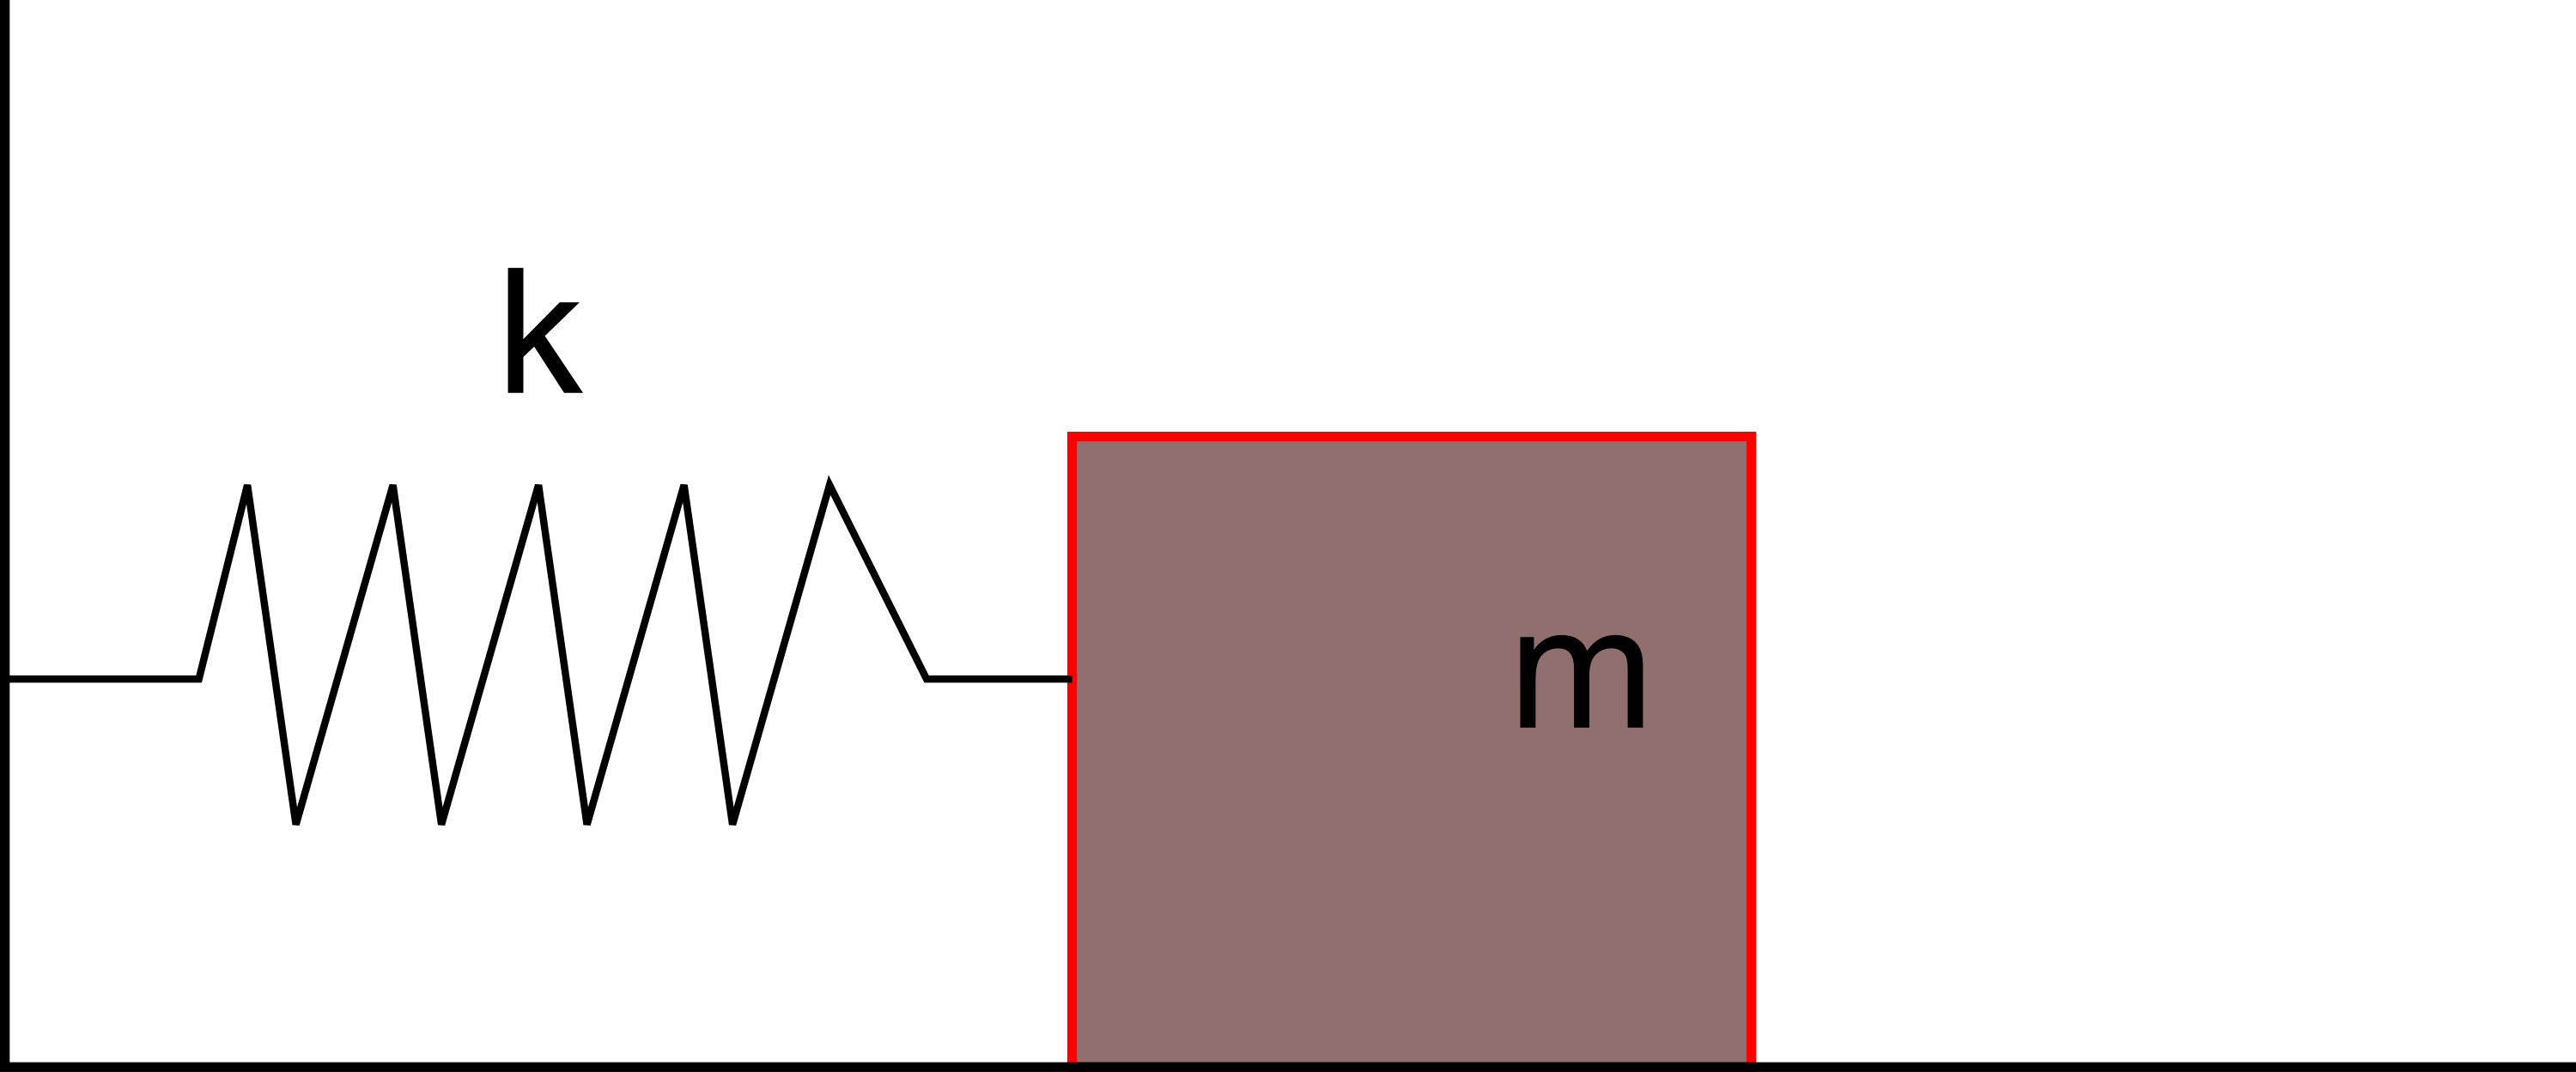
\includegraphics[width=6cm]{img/springMassStatic}}
  \only<2>{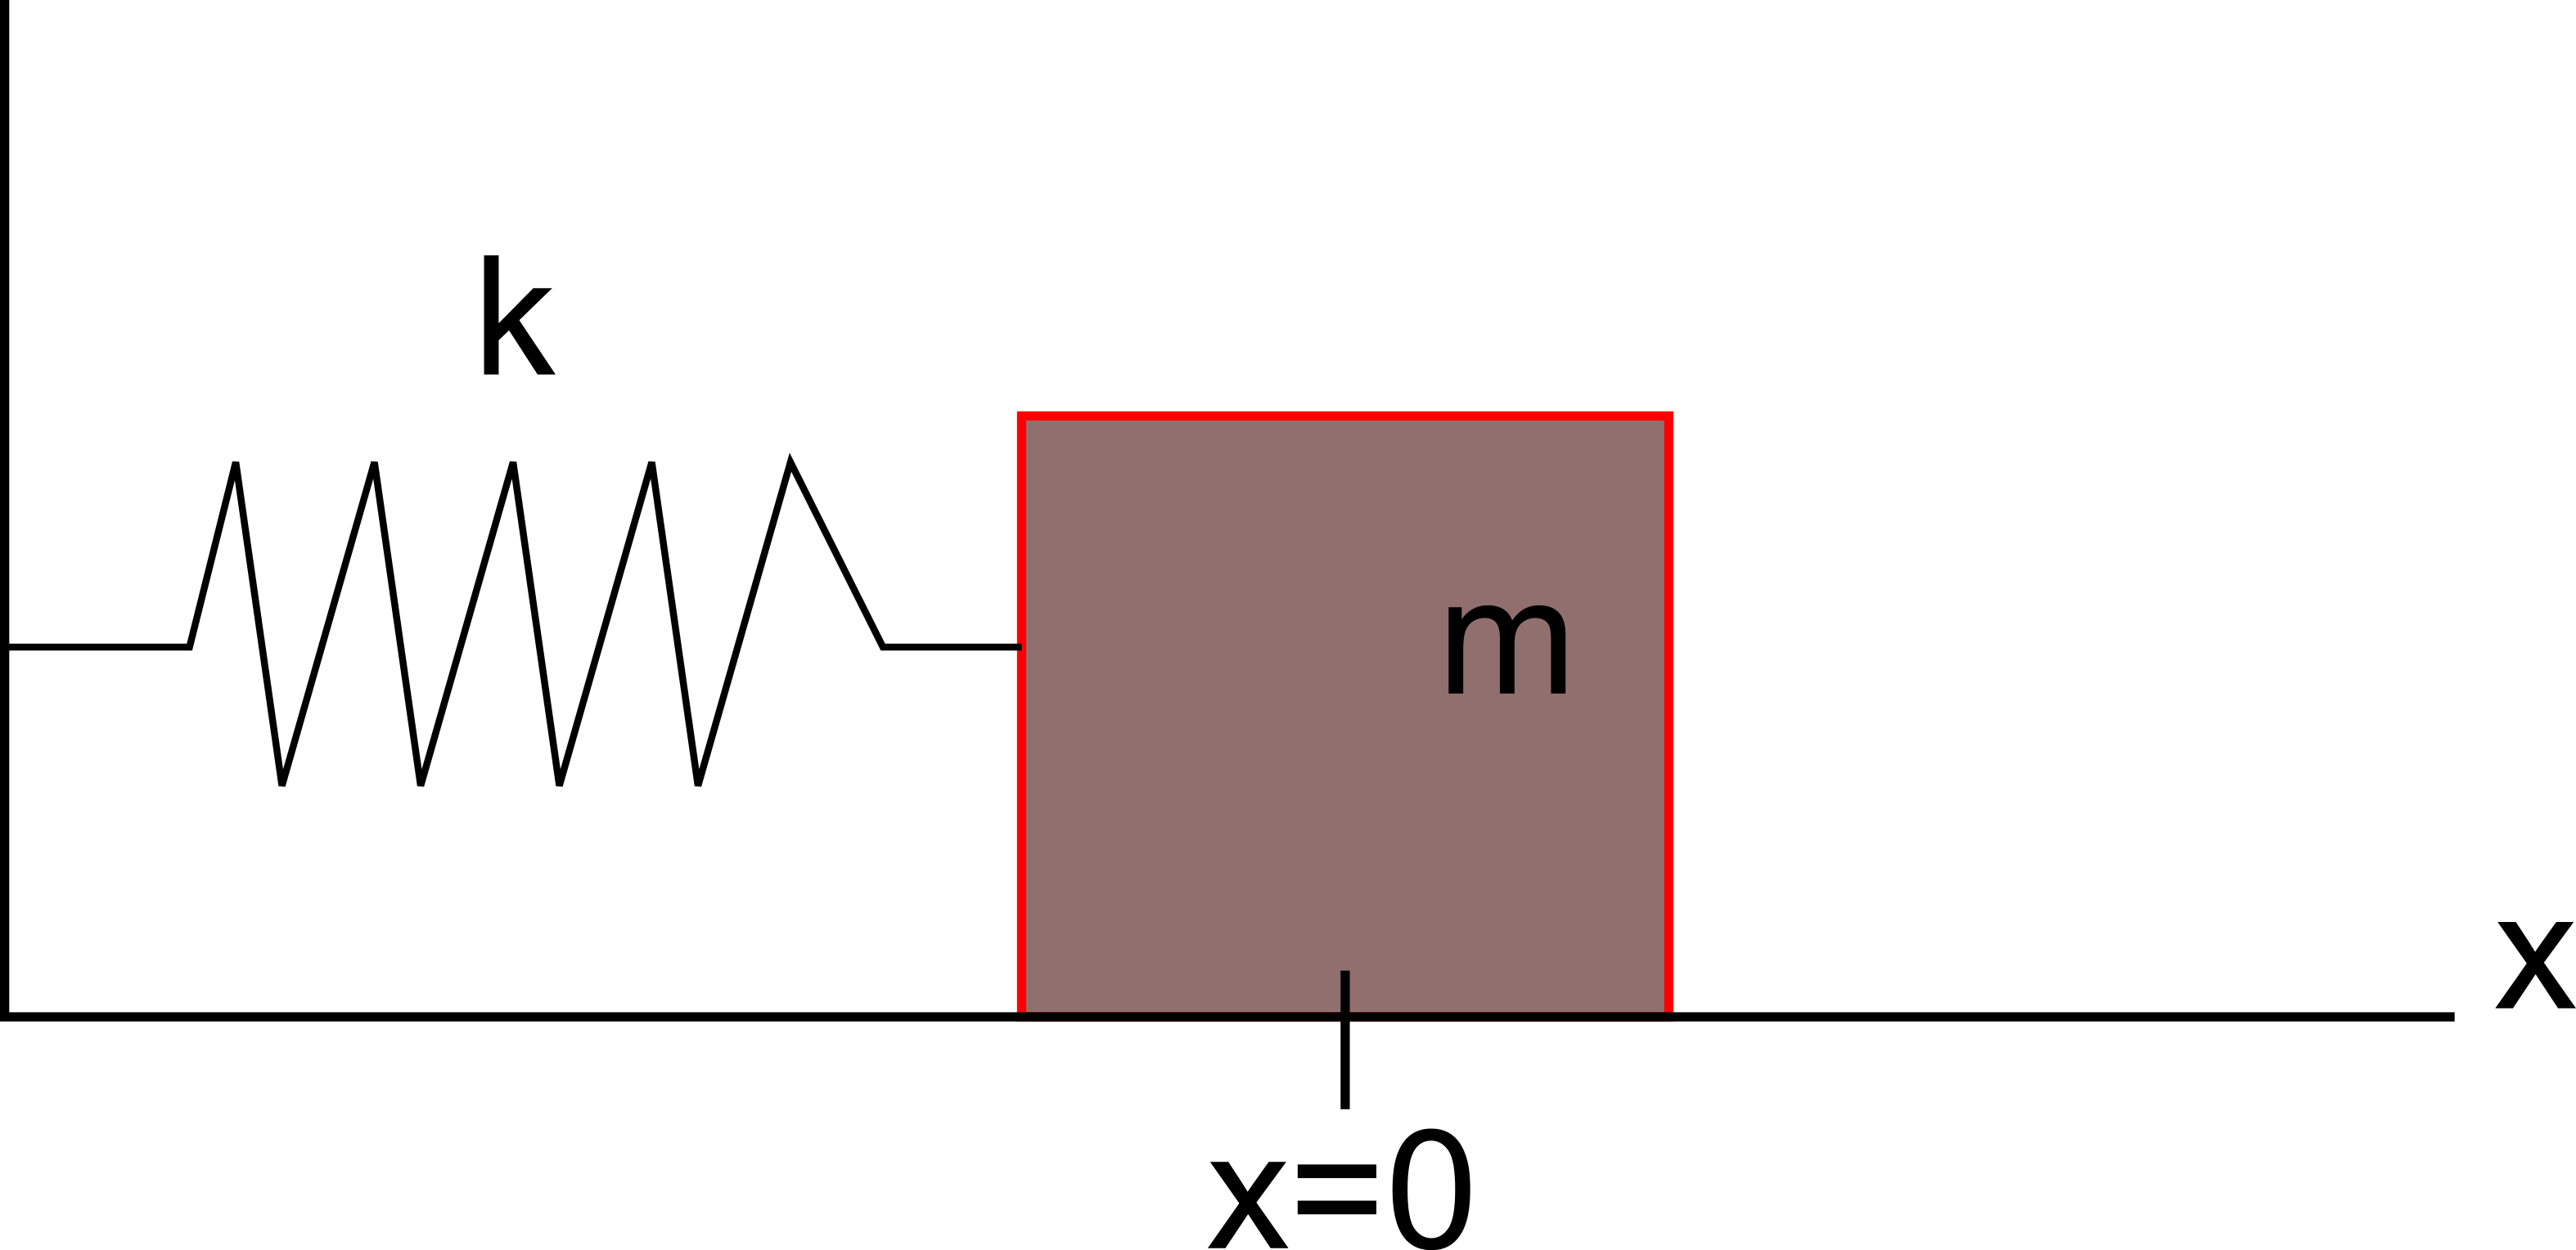
\includegraphics[width=6cm]{img/springMassStaticCoordinates}}
  \only<3>{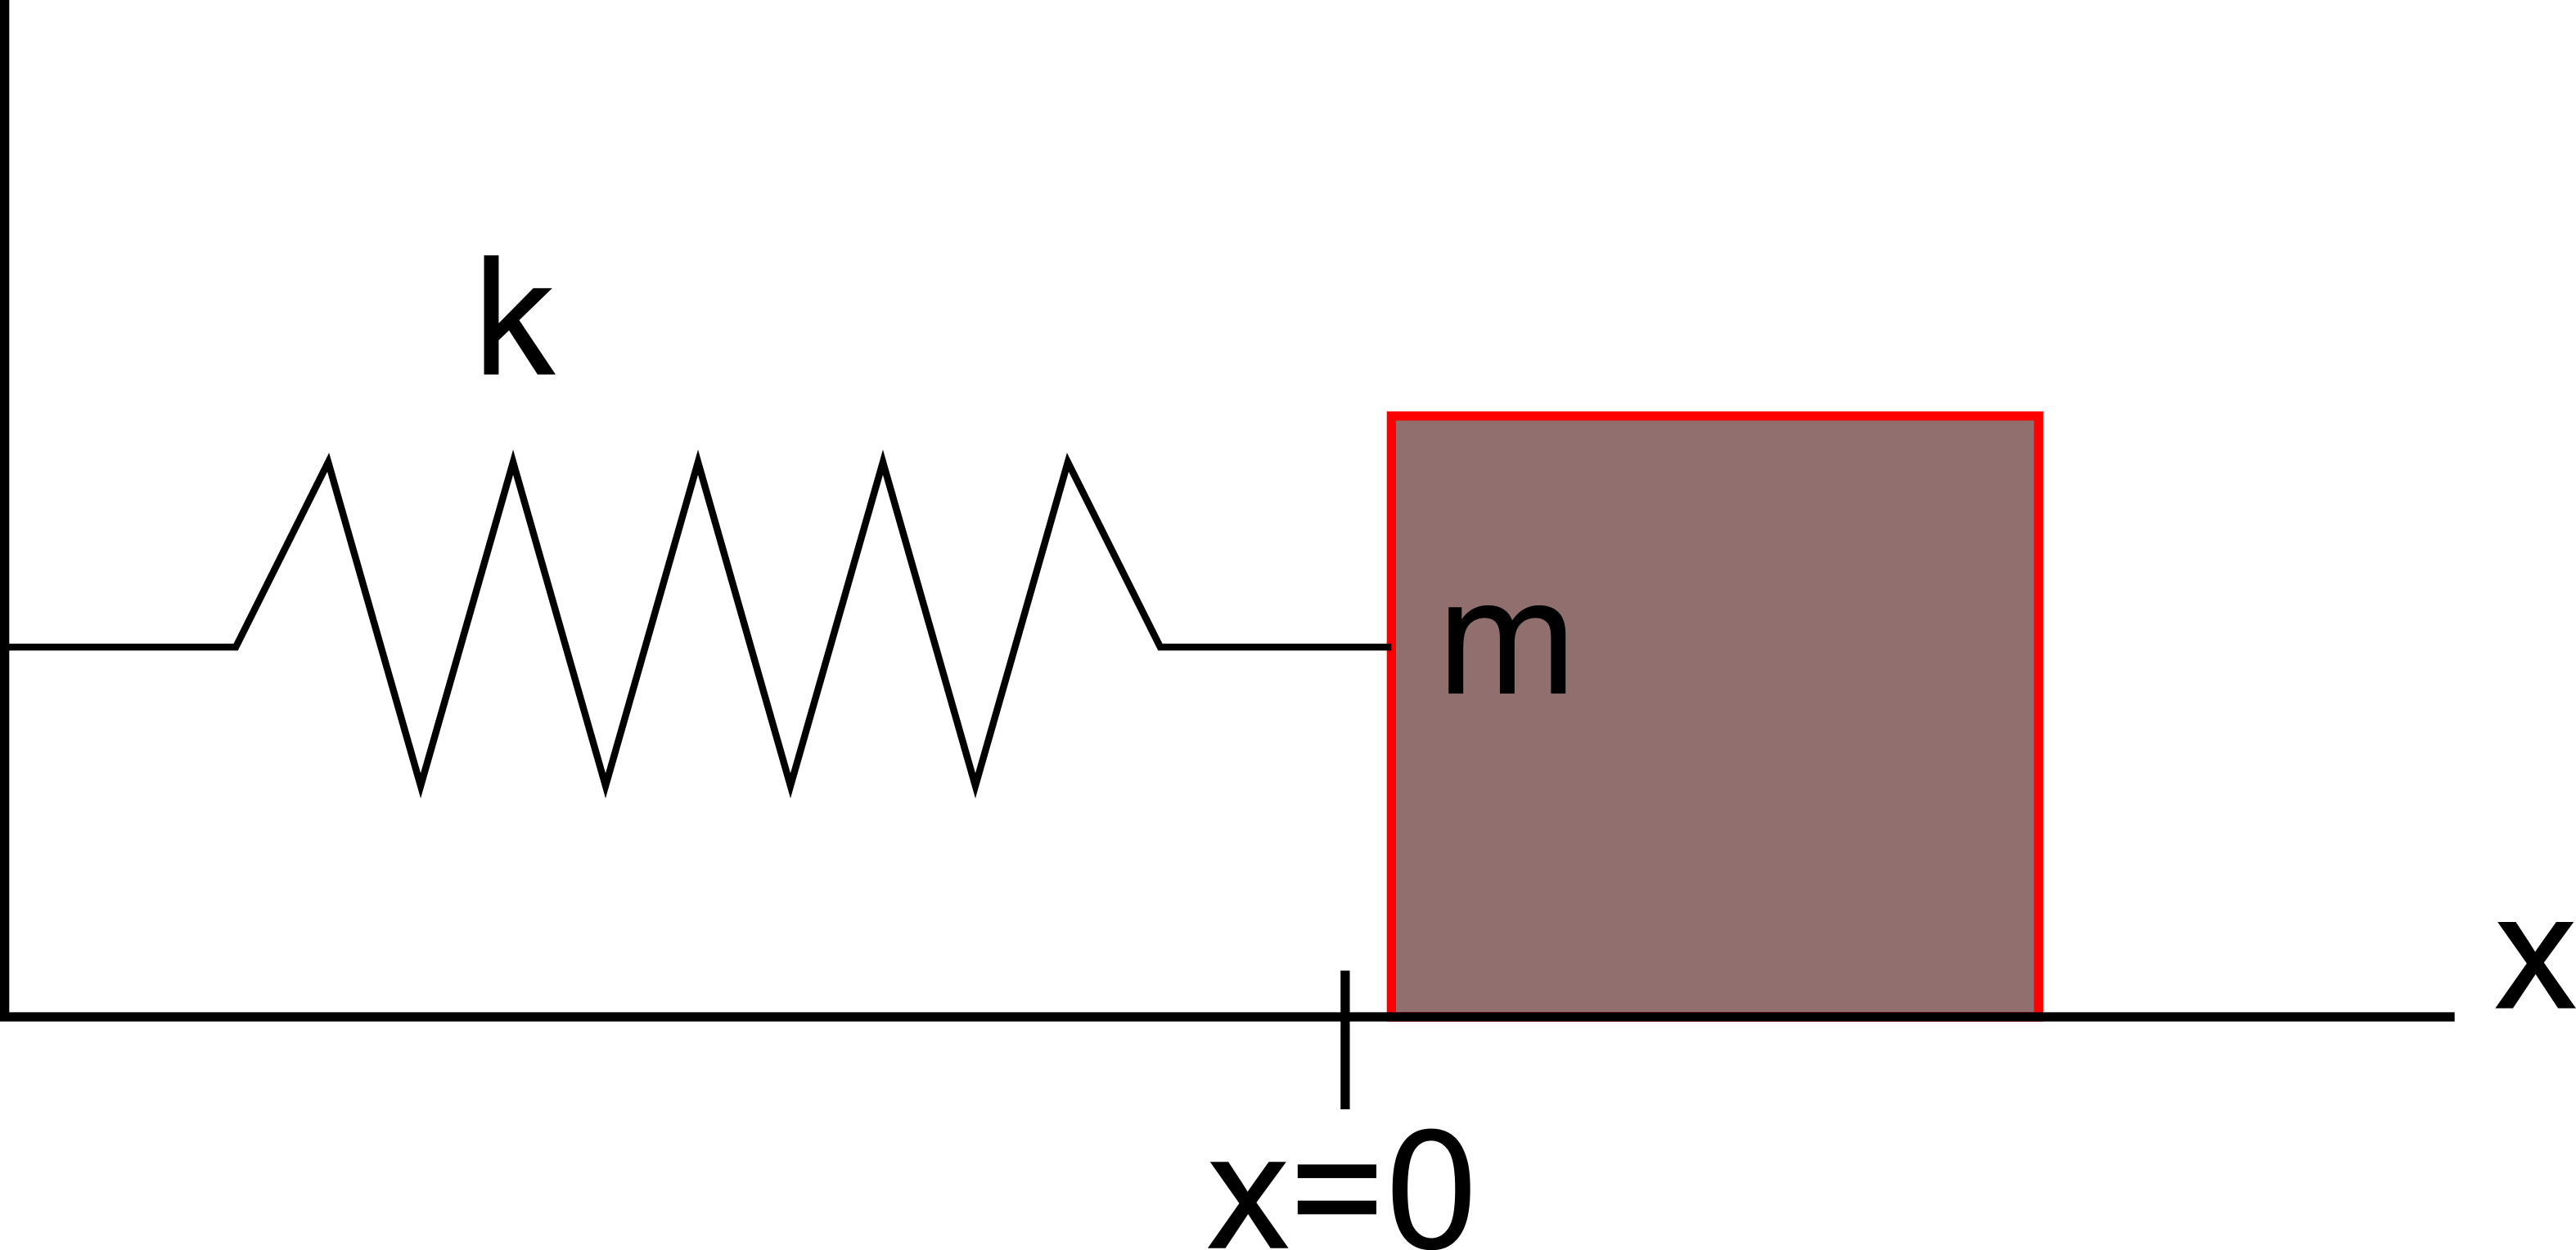
\includegraphics[width=6cm]{img/springMassDynamic}}
  \only<4->{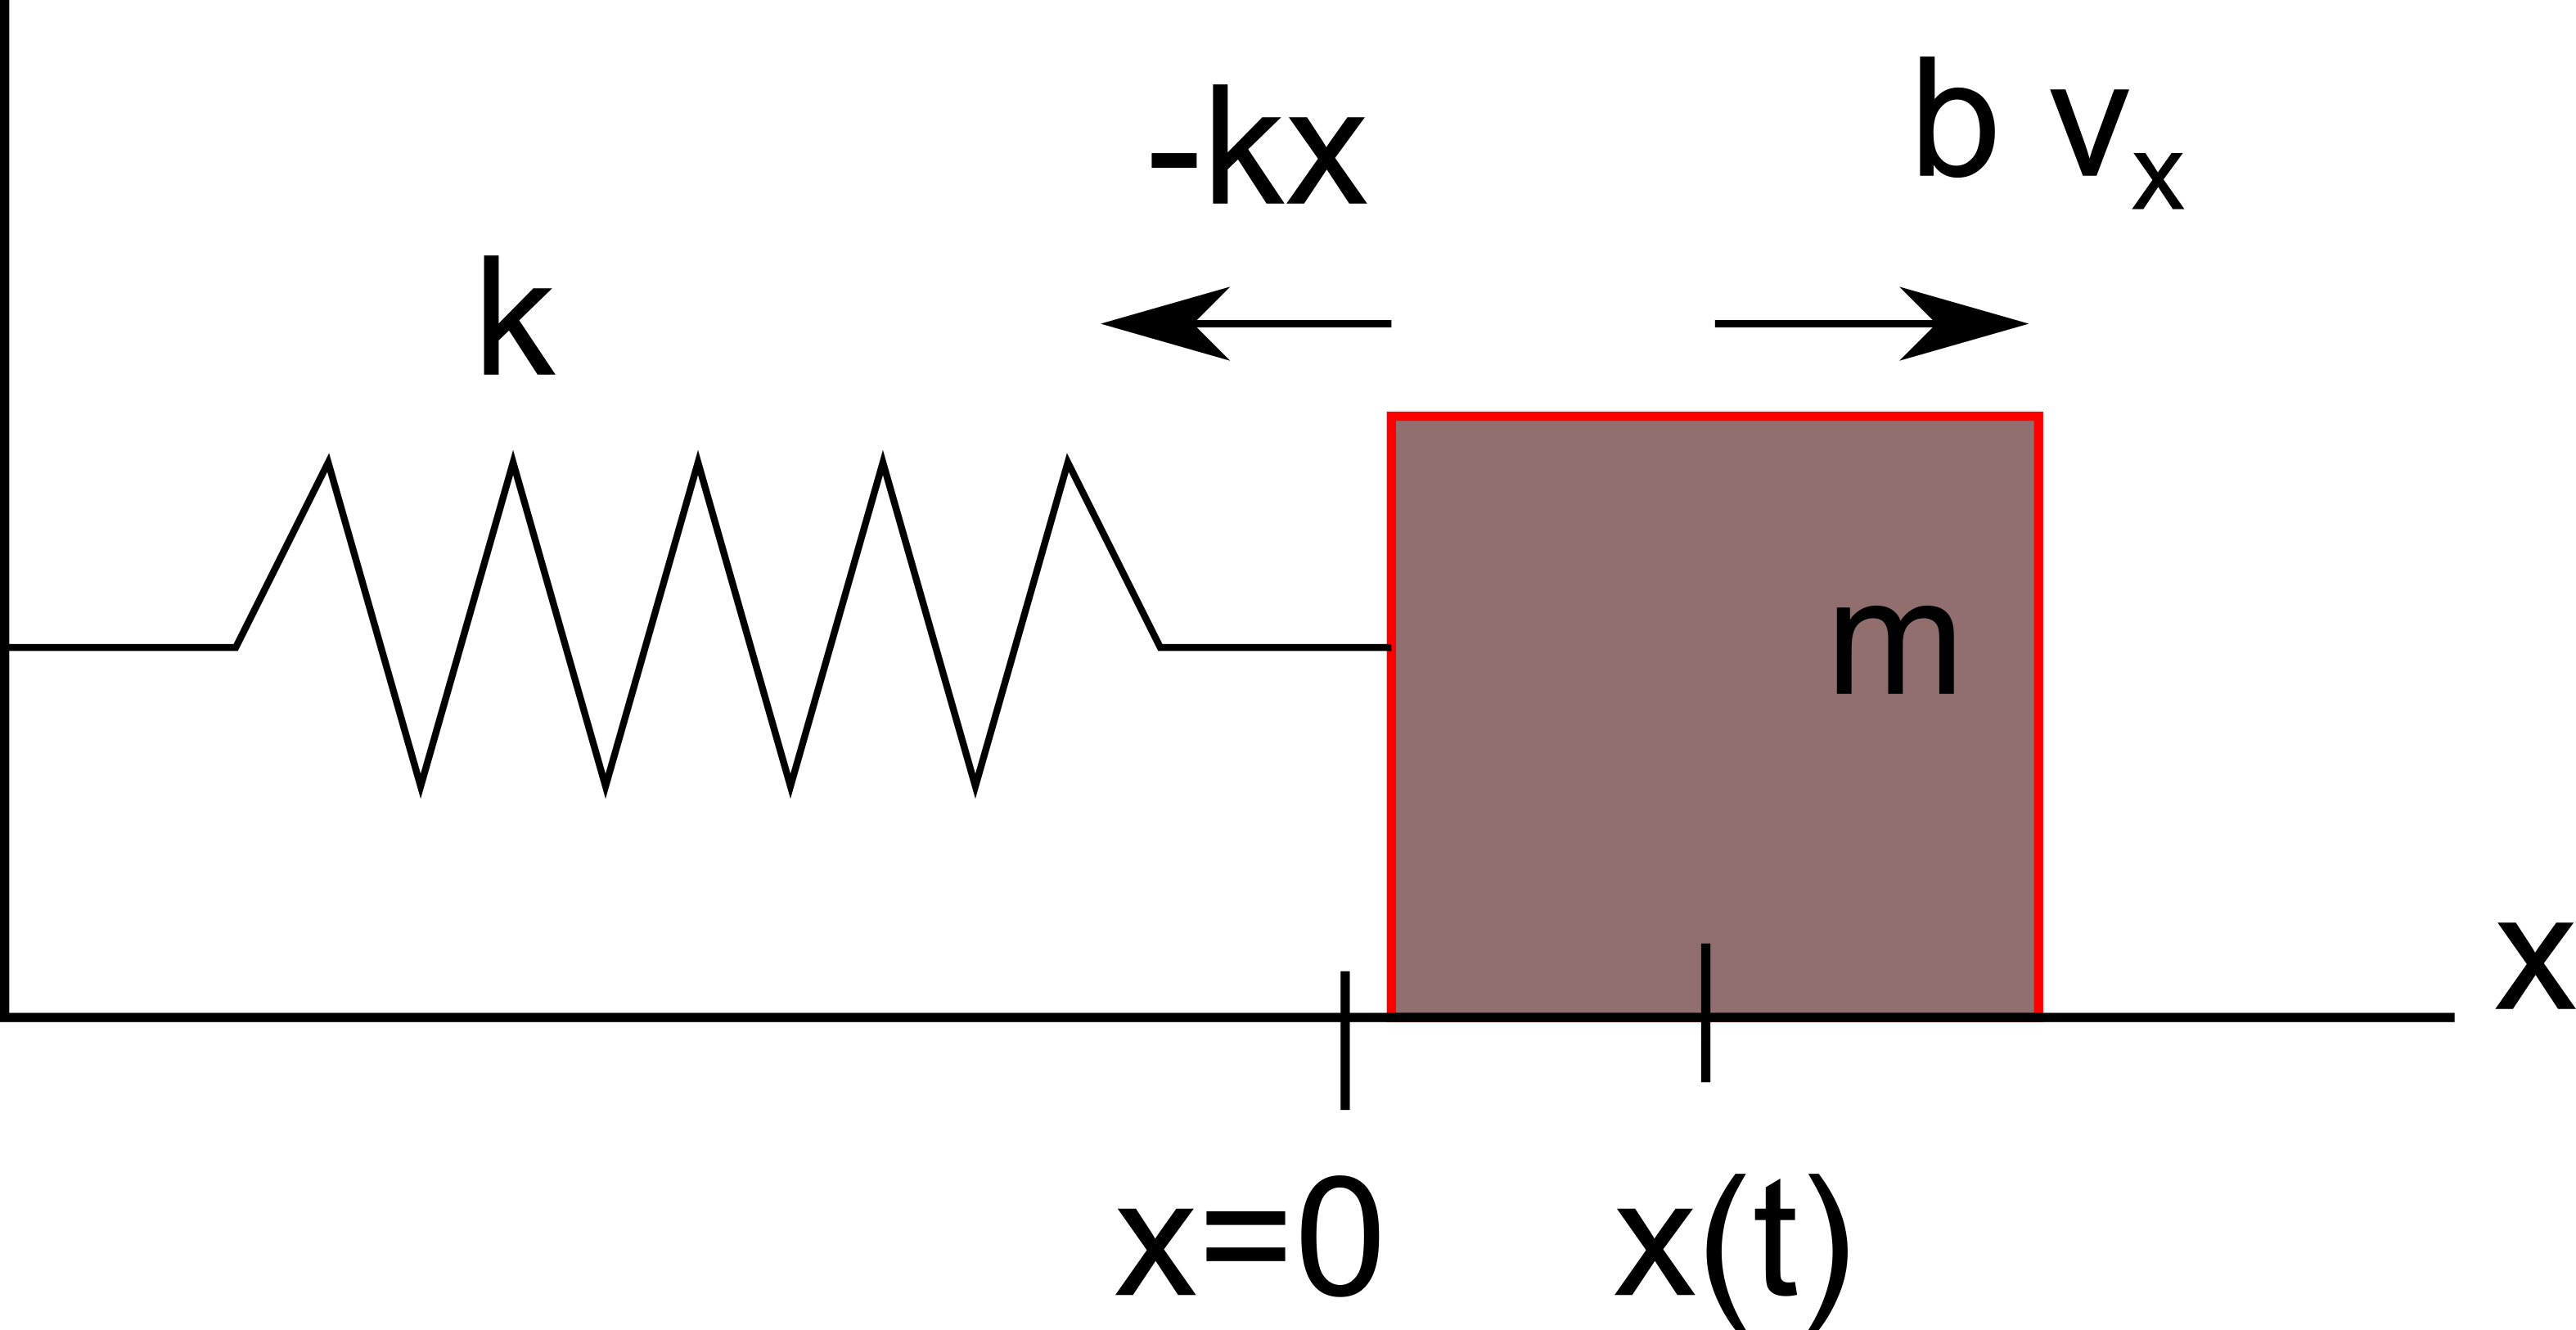
\includegraphics[width=6cm]{img/springMassDynamicVectors}}

  \uncover<4->{%
    Newton's Second Law:
    \begin{eqnarray*}
      \frac{d}{dt} \lp m \vec{v} \rp & = & \sum_i \vec{F}_i \\
      & = & -kx - bv_x 
    \end{eqnarray*}
    or
    \begin{eqnarray*}
      mx'' + bx' + kx & = & 0.
    \end{eqnarray*}

    If $b=0$ it is an ``\textbf{undamped''} system, otherwise it is ``\textbf{damped}.''
  }

\end{frame}


\begin{frame}
  \frametitle{Example}

  A mass of 2 kg is resting on an horizontal table and is attached to
  a linear spring which has a spring constant of 3 N/m. The force of
  friction is 1.5 times the velocity. The block is pulled to the left
  0.5m and let go from rest. Find the governing equation.

  \uncover<2->
  {
    \begin{eqnarray*}
      2 x'' + 1.5 x' + 3x & = & 0, \\
      x(0) & = & -.5m, \\
      x'(0) & = & 0 m/s.
    \end{eqnarray*}

    Need two initial conditions!
  }

\end{frame}


\begin{frame}
  \frametitle{Lots of variations}

  \begin{itemize}
  \item Could say that the spring stretched .25 m when 2N is applied.
  \item Could say that the force of friction is 0.5N when it is moving
    .3 m/s. 
  \end{itemize}

  See example on p. 197.

\end{frame}

\subsection{Undamped Systems}

\iftoggle{clicker}{%
\begin{frame}
  \frametitle{Clicker Quiz}

      \ifnum\value{clickerQuiz}=1{%

        \vfill

        Suppose that the spring/mass system has no friction,
        $b=0$, 
        \begin{eqnarray*}
          m x'' + kx & = & 0.
        \end{eqnarray*}        
        What kind of behavior do you expect?

        \vfill

        \begin{tabular}{ll}
          A: & Infinite, perfect oscillations until the end of time. \\
             & (or the end of today's class whichever comes first)  \\
          B: & Oscillations slowly dieing out.  \\
          C: & Oscillations with slow but steady decay \\
          D  & Oscillations with exponential decay
        \end{tabular}


        \vfill

      }\fi

      \ifnum\value{clickerQuiz}=2{%

        \vfill
        Suppose that the spring/mass system has no friction,
        $b=0$, 
        \begin{eqnarray*}
          m x'' + kx & = & 0.
        \end{eqnarray*}        
        What kind of behavior do you expect?

        \vfill

        \begin{tabular}{ll}
          A: & Infinite, perfect oscillations until the end of time. \\
             & (or the end of today's class whichever comes first)  \\
          B: & Oscillations slowly dieing out.  \\
          C: & Oscillations with slow but steady decay \\
          D  & Oscillations with exponential decay
        \end{tabular}


        \vfill

     }\fi
   
     \ifnum\value{clickerQuiz}=3{%
        Suppose that the spring/mass system has no friction,
        $b=0$,
        \begin{eqnarray*}
          m x'' + kx & = & 0.
        \end{eqnarray*}
        What kind of behavior do you expect?

        \vfill

        \begin{tabular}{ll}
          A: & Infinite, perfect oscillations until the end of time. \\
             & (or the end of today's class whichever comes first)  \\
          B: & Oscillations slowly dieing out.  \\
          C: & Oscillations with slow but steady decay \\
          D  & Oscillations with exponential decay
        \end{tabular}


        \vfill

    }\fi
  

\end{frame}
}



\begin{frame}
  \frametitle{Special Case}

  No friction, $b=0$: \textit{(Use your intuition!)} 
  \begin{eqnarray*}
    m x'' + kx & = & 0.
  \end{eqnarray*}

  \uncover<2->
  {
    Assume solutions of the form 
    \begin{eqnarray*}
      x & = & C_1 \cos(\redText{\omega} t) + C_2 \sin(\redText{\omega} t) \\
      \uncover<3->
      {
        x' & = & -\redText{\omega} C_1 \sin(\redText{\omega} t) + \redText{\omega} C_2 \cos(\redText{\omega} t) \\
      }
      \uncover<4->
      {
        x'' & = & -\redText{\omega}^2 C_1 \cos(\redText{\omega} t) - \redText{\omega}^2 C_2 \sin(\redText{\omega} t) \\
      }
    \end{eqnarray*}
  }

\end{frame}



\begin{frame}
  \frametitle{Special Case}

  No friction, $b=0$:
  \begin{eqnarray*}
    m x'' + kx & = & 0.
  \end{eqnarray*}

  \uncover<2->
  {
    \begin{eqnarray*}
      0 & = & mx''+kx \\
        & = & - m\redText{\omega}^2 C_1 \cos(\redText{\omega} t) - m\redText{\omega}^2 C_2 \sin(\redText{\omega} t) \\
        &   & + k C_1 \cos(\redText{\omega} t) + k C_2 \sin(\redText{\omega} t)\\
        & = & \lp -m \redText{\omega}^2 + k \rp C_1 \cos(\redText{\omega} t) +
              \lp -m \redText{\omega}^2 + k \rp C_2 \sin(\redText{\omega} t)
    \end{eqnarray*}
  }

  \uncover<3->
  {
    \begin{eqnarray*}
      \Rightarrow \redText{\omega} & = & \pm \sqrt{\frac{k}{m}}.
    \end{eqnarray*}
  }

  \vfill

\end{frame}


\begin{frame}
  \frametitle{Special Case}

  No friction, $b=0$:
  \begin{eqnarray*}
    m x'' + kx & = & 0.
  \end{eqnarray*}

  \begin{eqnarray*}
    x & = & C_1 \cos\lp\sqrt{\frac{k}{m}} t\rp +
    C_2 \sin\lp\sqrt{\frac{k}{m}} t\rp \\
    & = & A \cdot \cos\lp \sqrt{\frac{k}{m}} t - \delta \rp.
  \end{eqnarray*}

  Period = \blueText{T},
  \begin{eqnarray*}
    \sqrt{\frac{k}{m}} \blueText{T} & = & 2\pi, \\
    \Rightarrow \blueText{T} & = & 2 \pi \sqrt{\frac{m}{k}}.
  \end{eqnarray*}

\end{frame}


\begin{frame}
  \frametitle{Example}

  An horizontal spring/mass system is to be constructed using a 2 kg
  mass. What spring constant should be used so that it oscillates at 3
  oscillations per second?

  \begin{eqnarray*}
    2 x'' + \redText{k}x & = & 0 \\
    x & = & A \cdot \cos\lp \sqrt{\frac{\redText{k}}{2}} t - \delta \rp \\
  \end{eqnarray*}

  \uncover<2->
  {
    3 oscillations per second means that
    \begin{eqnarray*}
      \sqrt{\frac{\redText{k}}{2}} \lp \frac{1}{3} \rp & = & 2 \pi, \\
      \redText{k} & = & 72 \pi^2~\mathrm{N/m}.
    \end{eqnarray*}
  }

\end{frame}

\subsection{RCL Circuits}

\begin{frame}
  \frametitle{RCL Circuit}

  See pp. 202-204 for more information about LRC circuits.

  \begin{columns}
    \column{.5\textwidth}
    % Graphic for TeX using PGF
% Title: /home/black/write/class/de/math232-12/ODE-Recitation-Activities/notes/img/LRCcircuit.dia
% Creator: Dia v0.97.2
% CreationDate: Wed Sep 18 10:33:40 2013
% For: black
% \usepackage{tikz}
% The following commands are not supported in PSTricks at present
% We define them conditionally, so when they are implemented,
% this pgf file will use them.
\ifx\du\undefined
  \newlength{\du}
\fi
\setlength{\du}{15\unitlength}
\begin{tikzpicture}
\pgftransformxscale{0.500000}
\pgftransformyscale{-0.500000}
\definecolor{dialinecolor}{rgb}{0.000000, 0.000000, 0.000000}
\pgfsetstrokecolor{dialinecolor}
\definecolor{dialinecolor}{rgb}{1.000000, 1.000000, 1.000000}
\pgfsetfillcolor{dialinecolor}
\pgfsetlinewidth{0.100000\du}
\pgfsetdash{}{0pt}
\pgfsetdash{}{0pt}
\pgfsetbuttcap
\pgfsetmiterjoin
\pgfsetlinewidth{0.100000\du}
\pgfsetbuttcap
\pgfsetmiterjoin
\pgfsetdash{}{0pt}
\definecolor{dialinecolor}{rgb}{0.000000, 0.000000, 0.000000}
\pgfsetstrokecolor{dialinecolor}
\draw (2.900000\du,9.550000\du)--(2.900000\du,10.800000\du);
\pgfsetbuttcap
\pgfsetmiterjoin
\pgfsetdash{}{0pt}
\definecolor{dialinecolor}{rgb}{0.000000, 0.000000, 0.000000}
\pgfsetstrokecolor{dialinecolor}
\draw (2.400000\du,10.800000\du)--(3.400000\du,10.800000\du);
\pgfsetbuttcap
\pgfsetmiterjoin
\pgfsetdash{}{0pt}
\definecolor{dialinecolor}{rgb}{0.000000, 0.000000, 0.000000}
\pgfsetstrokecolor{dialinecolor}
\draw (2.650000\du,11.300000\du)--(3.150000\du,11.300000\du);
\pgfsetbuttcap
\pgfsetmiterjoin
\pgfsetdash{}{0pt}
\definecolor{dialinecolor}{rgb}{0.000000, 0.000000, 0.000000}
\pgfsetstrokecolor{dialinecolor}
\draw (3.150000\du,10.050000\du)--(3.150000\du,10.550000\du);
\pgfsetbuttcap
\pgfsetmiterjoin
\pgfsetdash{}{0pt}
\definecolor{dialinecolor}{rgb}{0.000000, 0.000000, 0.000000}
\pgfsetstrokecolor{dialinecolor}
\draw (3.025000\du,10.300000\du)--(3.275000\du,10.300000\du);
\pgfsetbuttcap
\pgfsetmiterjoin
\pgfsetdash{}{0pt}
\definecolor{dialinecolor}{rgb}{0.000000, 0.000000, 0.000000}
\pgfsetstrokecolor{dialinecolor}
\draw (2.900000\du,11.300000\du)--(2.900000\du,12.550000\du);
\pgfsetlinewidth{0.100000\du}
\pgfsetdash{}{0pt}
\pgfsetdash{}{0pt}
\pgfsetbuttcap
\pgfsetmiterjoin
\pgfsetlinewidth{0.100000\du}
\pgfsetbuttcap
\pgfsetmiterjoin
\pgfsetdash{}{0pt}
\definecolor{dialinecolor}{rgb}{0.000000, 0.000000, 0.000000}
\pgfsetstrokecolor{dialinecolor}
\draw (4.350000\du,7.900000\du)--(5.595000\du,7.900000\du)--(5.733333\du,7.400000\du)--(6.010000\du,8.400000\du)--(6.286667\du,7.400000\du)--(6.563333\du,8.400000\du)--(6.840000\du,7.400000\du)--(7.116667\du,8.400000\du)--(7.255000\du,7.900000\du)--(8.500000\du,7.900000\du);
\pgfsetlinewidth{0.100000\du}
\pgfsetdash{}{0pt}
\pgfsetdash{}{0pt}
\pgfsetbuttcap
\pgfsetmiterjoin
\pgfsetlinewidth{0.100000\du}
\pgfsetbuttcap
\pgfsetmiterjoin
\pgfsetdash{}{0pt}
\definecolor{dialinecolor}{rgb}{0.000000, 0.000000, 0.000000}
\pgfsetstrokecolor{dialinecolor}
\pgfpathmoveto{\pgfpoint{9.800000\du}{8.950000\du}}
\pgfpathlineto{\pgfpoint{9.800000\du}{9.790000\du}}
\pgfpathcurveto{\pgfpoint{10.300000\du}{9.685000\du}}{\pgfpoint{10.800000\du}{9.580000\du}}{\pgfpoint{10.800000\du}{10.105000\du}}
\pgfpathcurveto{\pgfpoint{10.800000\du}{10.630000\du}}{\pgfpoint{9.800000\du}{10.735000\du}}{\pgfpoint{9.800000\du}{10.420000\du}}
\pgfpathcurveto{\pgfpoint{9.800000\du}{10.105000\du}}{\pgfpoint{10.800000\du}{10.210000\du}}{\pgfpoint{10.800000\du}{10.735000\du}}
\pgfpathcurveto{\pgfpoint{10.800000\du}{11.260000\du}}{\pgfpoint{9.800000\du}{11.365000\du}}{\pgfpoint{9.800000\du}{11.050000\du}}
\pgfpathcurveto{\pgfpoint{9.800000\du}{10.735000\du}}{\pgfpoint{10.800000\du}{10.840000\du}}{\pgfpoint{10.800000\du}{11.365000\du}}
\pgfpathcurveto{\pgfpoint{10.800000\du}{11.890000\du}}{\pgfpoint{9.800000\du}{11.995000\du}}{\pgfpoint{9.800000\du}{11.680000\du}}
\pgfpathcurveto{\pgfpoint{9.800000\du}{11.365000\du}}{\pgfpoint{10.800000\du}{11.470000\du}}{\pgfpoint{10.800000\du}{11.995000\du}}
\pgfpathcurveto{\pgfpoint{10.800000\du}{12.520000\du}}{\pgfpoint{10.050000\du}{12.415000\du}}{\pgfpoint{9.800000\du}{12.310000\du}}
\pgfpathlineto{\pgfpoint{9.800000\du}{13.150000\du}}
\pgfusepath{stroke}
\pgfsetlinewidth{0.100000\du}
\pgfsetdash{}{0pt}
\pgfsetdash{}{0pt}
\pgfsetbuttcap
\pgfsetmiterjoin
\pgfsetlinewidth{0.100000\du}
\pgfsetbuttcap
\pgfsetmiterjoin
\pgfsetdash{}{0pt}
\definecolor{dialinecolor}{rgb}{0.000000, 0.000000, 0.000000}
\pgfsetstrokecolor{dialinecolor}
\draw (4.800000\du,14.900000\du)--(6.000000\du,14.900000\du);
\pgfsetbuttcap
\pgfsetmiterjoin
\pgfsetdash{}{0pt}
\definecolor{dialinecolor}{rgb}{0.000000, 0.000000, 0.000000}
\pgfsetstrokecolor{dialinecolor}
\draw (6.000000\du,14.400000\du)--(6.000000\du,15.400000\du);
\pgfsetbuttcap
\pgfsetmiterjoin
\pgfsetdash{}{0pt}
\definecolor{dialinecolor}{rgb}{0.000000, 0.000000, 0.000000}
\pgfsetstrokecolor{dialinecolor}
\draw (6.600000\du,14.400000\du)--(6.600000\du,15.400000\du);
\pgfsetbuttcap
\pgfsetmiterjoin
\pgfsetdash{}{0pt}
\definecolor{dialinecolor}{rgb}{0.000000, 0.000000, 0.000000}
\pgfsetstrokecolor{dialinecolor}
\draw (6.600000\du,14.900000\du)--(7.800000\du,14.900000\du);
\pgfsetlinewidth{0.100000\du}
\pgfsetdash{}{0pt}
\pgfsetdash{}{0pt}
\pgfsetmiterjoin
\pgfsetbuttcap
{
\definecolor{dialinecolor}{rgb}{0.000000, 0.000000, 0.000000}
\pgfsetfillcolor{dialinecolor}
% was here!!!
{\pgfsetcornersarced{\pgfpoint{0.000000\du}{0.000000\du}}\definecolor{dialinecolor}{rgb}{0.000000, 0.000000, 0.000000}
\pgfsetstrokecolor{dialinecolor}
\draw (8.500000\du,7.900000\du)--(9.800000\du,7.900000\du)--(9.800000\du,8.950000\du);
}}
\pgfsetlinewidth{0.100000\du}
\pgfsetdash{}{0pt}
\pgfsetdash{}{0pt}
\pgfsetmiterjoin
\pgfsetbuttcap
{
\definecolor{dialinecolor}{rgb}{0.000000, 0.000000, 0.000000}
\pgfsetfillcolor{dialinecolor}
% was here!!!
{\pgfsetcornersarced{\pgfpoint{0.000000\du}{0.000000\du}}\definecolor{dialinecolor}{rgb}{0.000000, 0.000000, 0.000000}
\pgfsetstrokecolor{dialinecolor}
\draw (2.900000\du,9.550000\du)--(2.900000\du,7.900000\du)--(4.350000\du,7.900000\du);
}}
\pgfsetlinewidth{0.100000\du}
\pgfsetdash{}{0pt}
\pgfsetdash{}{0pt}
\pgfsetmiterjoin
\pgfsetbuttcap
{
\definecolor{dialinecolor}{rgb}{0.000000, 0.000000, 0.000000}
\pgfsetfillcolor{dialinecolor}
% was here!!!
{\pgfsetcornersarced{\pgfpoint{0.000000\du}{0.000000\du}}\definecolor{dialinecolor}{rgb}{0.000000, 0.000000, 0.000000}
\pgfsetstrokecolor{dialinecolor}
\draw (9.800000\du,13.150000\du)--(9.800000\du,13.150000\du)--(9.800000\du,14.900000\du)--(7.800000\du,14.900000\du);
}}
\pgfsetlinewidth{0.100000\du}
\pgfsetdash{}{0pt}
\pgfsetdash{}{0pt}
\pgfsetmiterjoin
\pgfsetbuttcap
{
\definecolor{dialinecolor}{rgb}{0.000000, 0.000000, 0.000000}
\pgfsetfillcolor{dialinecolor}
% was here!!!
{\pgfsetcornersarced{\pgfpoint{0.000000\du}{0.000000\du}}\definecolor{dialinecolor}{rgb}{0.000000, 0.000000, 0.000000}
\pgfsetstrokecolor{dialinecolor}
\draw (2.900000\du,12.550000\du)--(2.900000\du,14.900000\du)--(4.800000\du,14.900000\du);
}}
% setfont left to latex
\definecolor{dialinecolor}{rgb}{0.000000, 0.000000, 0.000000}
\pgfsetstrokecolor{dialinecolor}
\node[anchor=west] at (6.050000\du,6.600000\du){R};
% setfont left to latex
\definecolor{dialinecolor}{rgb}{0.000000, 0.000000, 0.000000}
\pgfsetstrokecolor{dialinecolor}
\node[anchor=west] at (5.865000\du,17.055000\du){C};
% setfont left to latex
\definecolor{dialinecolor}{rgb}{0.000000, 0.000000, 0.000000}
\pgfsetstrokecolor{dialinecolor}
\node[anchor=west] at (-1.080000\du,11.360000\du){V(t)};
% setfont left to latex
\definecolor{dialinecolor}{rgb}{0.000000, 0.000000, 0.000000}
\pgfsetstrokecolor{dialinecolor}
\node[anchor=west] at (7.450000\du,16.200000\du){};
% setfont left to latex
\definecolor{dialinecolor}{rgb}{0.000000, 0.000000, 0.000000}
\pgfsetstrokecolor{dialinecolor}
\node[anchor=west] at (11.315000\du,11.455000\du){L};
\end{tikzpicture}


    \column{.5\textwidth}
    Voltage drops: \\
    \begin{tabular}{l@{~$=$~}l}
      Resistor & $RI$ \\
      Inductor & $LI'$ \\
      Capacitor & $\frac{Q}{C}$.
    \end{tabular}
  \end{columns}

  \uncover<2->{
    \begin{eqnarray*}
      L I' + RI + Q/C & = & v(t) \\
      L Q'' + RQ' + Q'/C & = & v(t).
    \end{eqnarray*}
  }

\end{frame}



% LocalWords:  Clarkson pausesection hideothersubsections DEs ODEs undamped kx
% LocalWords:  mx RCL

\part{Solutions-to-Second-Order-DEs}
\lecture{Solutions to Second Order DEs}{Solutions-to-Second-Order-DEs}
\section{Solutions to Second Order DEs}

\title{Ordinary Differential Equations}
\subtitle{Math 232 - Week 7, Day 3}
\date{14 Oct 2012}

\begin{frame}
  \titlepage
\end{frame}

\begin{frame}
  \frametitle{Outline}
  \tableofcontents[pausesection,hideothersubsections]
\end{frame}


\subsection{Solutions to Second Order DEs}


\begin{frame}
  \frametitle{What is a solution to a general second order DE?}

  Solutions to
  \begin{eqnarray*}
    a y'' + by' + cy & = & 0.
  \end{eqnarray*}

  \uncover<2->
  {
    Assume
    \begin{eqnarray*}
      y & = & A e^{rt}, \\
      y' & = & r A e^{rt}, \\
      y'' & = & r^2 A e^{rt}.
    \end{eqnarray*}
    (If it works I am done!)
  }

\end{frame}


\begin{frame}
  \frametitle{Substitute back into the equation}

  The original de:
  \begin{eqnarray*}
    a y'' + by' + cy & = & 0, \\
    a r^2 A e^{rt} + b r A e^{rt} + c A e^{rt} & = & 0 \\
    \uncover<2->
    {
      A e^{rt} \left[ a r^2 + br + c \right] & = & 0.
    }
  \end{eqnarray*}

  \uncover<3->
  {
    This is true if
    \begin{eqnarray*}
      r & = & \frac{-b \pm \sqrt{b^2-4ac}}{2a}.
    \end{eqnarray*}
  }

  \uncover<4->
  {
    Three cases: distinct real, repeated roots, complex roots.
  }

\end{frame}

\subsection{Real, Distinct Roots}

\begin{frame}
  \frametitle{Case 1: Distinct, Real Roots}

  \begin{eqnarray*}
    y & = & C_1 e^{r_1 t} + C_2 e^{r_2 t}.
  \end{eqnarray*}

\end{frame}


\begin{frame}
  \frametitle{Example}

  Find the general solution to
  \begin{eqnarray*}
    y'' - 5y' + 6y & = & 0.
  \end{eqnarray*}

  \uncover<2->
  {
    \begin{eqnarray*}
      r^2 - 5r + 6 & = & 0, \\
      (r-3)(r-2) & = & 0.
    \end{eqnarray*}

    The general solution is
    \begin{eqnarray*}
      y & = & C_1 e^{3t} + C_2 e^{2t}
    \end{eqnarray*}

  }

\end{frame}


\begin{frame}
  \frametitle{Example}

  Find the general solution to
  \begin{eqnarray*}
    y'' - 2y' - 8y & = & 0.
  \end{eqnarray*}

  \uncover<2->
  {
    \begin{eqnarray*}
      r^2 - 2r - 8 & = & 0, \\
      (r-4)(r+2) & = & 0.
    \end{eqnarray*}

    The general solution is
    \begin{eqnarray*}
      y & = & C_1 e^{4t} + C_2 e^{-2t}
    \end{eqnarray*}

  }

\end{frame}


\subsection{Case 2: Repeated Roots}

\begin{frame}
  \frametitle{Case 2: Repeated Roots}

  \begin{eqnarray*}
    y & = & C_1 e^{rt} + C_2 t e^{rt}
  \end{eqnarray*}


\end{frame}


\begin{frame}
  \frametitle{Example}

  \begin{eqnarray*}
    y'' + 6y' + 9y & = & 0.
  \end{eqnarray*}

  \uncover<2->
  {
    \begin{eqnarray*}
      r^2 + 6r + 9 & = & 0, \\
      (r+3)^2 & = & 0.
    \end{eqnarray*}

    The general solution is
    \begin{eqnarray*}
      y & = & C_1 e^{-3t} + C_2 t e^{-3t}
    \end{eqnarray*}

  }

\end{frame}


\begin{frame}
  \frametitle{Nomenclature}

  For spring/mass systems (or RCL circuits)
  \begin{itemize}
  \item Distinct real, negative roots - \textit{Over damped}
  \item One repeated root - \textit{Critically damped}
  \item Complex roots   - \textit{Under damped}
  \end{itemize}

\end{frame}

\begin{frame}
  \frametitle{Example}

  \begin{eqnarray*}
    y'' + 4y' + 4y & = & 0, \\
    y(0) & = & 0, \\
    y'(0) & = & 3.
  \end{eqnarray*}

  \uncover<2->
  {
    \begin{eqnarray*}
      r^2 + 4r + 4 & = & 0, \\
      (r+2)^2 & = & 0.
    \end{eqnarray*}

    The general solution is
    \begin{eqnarray*}
      y & = & C_1 e^{-2t} + C_2 t e^{-2t}
    \end{eqnarray*}

  }

\end{frame}



\begin{frame}
  \frametitle{Solve for the constants}

  \begin{eqnarray*}
    y(0) & = & 0 \\
    & = & C_1 \\
    \Rightarrow C_1 & = & 0.
  \end{eqnarray*}

  \begin{eqnarray*}
    y(t) & = & C_2 t e^{-2t} \\
    y'(t) & = & C_2 e^{-2t} - 2 C_2 t e^{-2t}, \\
    y'(0) & = & C_2 \\
    \Rightarrow C_2 & = & 3.
  \end{eqnarray*}

  The solution is
  \begin{eqnarray*}
    y_h & = & 3 t e^{-2t}.
  \end{eqnarray*}

\end{frame}

\subsection{More Examples}

\begin{frame}
  \frametitle{Example}

  Find the general solution to
  \begin{eqnarray*}
    y'' + 10 y' + 24y & = & 0.
  \end{eqnarray*}

  \uncover<2->
  {
    \begin{eqnarray*}
      r^2 + 10r + 24 & = & 0, \\
      r & = & \frac{-10\pm\sqrt{100-4(24)}}{2} \\
      & = & -4,~ -6.
    \end{eqnarray*}

    The general solution is
    \begin{eqnarray*}
      y & = & C_1 e^{-4t} + C_2 e^{-6t}
    \end{eqnarray*}

  }
  

\end{frame}

\begin{frame}
  \frametitle{Linear Independence}

  Question: Are the functions linear independent?

  \uncover<2->
  {

    If we have $n$-derivatives we need $n$ linearly independent
    functions:
    \begin{eqnarray*}
      \mathrm{det}\arrayTwo{e^{-4t}}{e^{-6t}}{-4e^{-4t}}{-6e^{-6t}} 
      & = & -2 e^{-10t}.
    \end{eqnarray*}

  }
  
\end{frame}


\begin{frame}
  \frametitle{Example}

  Find the general solution to
  \begin{eqnarray*}
    y'' + y' - 2y & = & 0, \\
    y(0) & = & 1, \\
    y'(0) & = & 2.
  \end{eqnarray*}

  \uncover<2->
  {
    \begin{eqnarray*}
      r^2 + r - 2 & = & 0, \\
      (r-1)(r+2) & = & 0.
    \end{eqnarray*}

    The general solution is
    \begin{eqnarray*}
      y & = & C_1 e^{-2t} + C_2 e^{t}
    \end{eqnarray*}

  }
  

\end{frame}

\begin{frame}
  \frametitle{Find The Specific Solution}

  Apply the initial condition:
  \begin{eqnarray*}
    y(0) & = & C_1 + C_2 \\
    y'(0) & = & -2C_1 + C_2
  \end{eqnarray*}

  \begin{eqnarray*}
    \startRowOpsTwo
    \oneRowOpsTwo{1}{1}{1}
    \oneRowOpsTwo{-2}{1}{2}
    \stopRowOps \\
    \Rightarrow
    \startRowOpsTwo
    \oneRowOpsTwo{1}{0}{-\frac{1}{3}}
    \oneRowOpsTwo{0}{1}{\frac{4}{3}}
    \stopRowOps
  \end{eqnarray*}

  So the solution is
  \begin{eqnarray*}
    y & = & -\frac{1}{3} e^{-2t} + \frac{4}{3} e^{t}.
  \end{eqnarray*}
  

\end{frame}


\begin{frame}
  \frametitle{Higher Order Derivatives}

  No reason to stop at two derivatives! Find the general solution to 
  \begin{eqnarray*}
    y''' + 2 y'' - y' - 2y & = & 0.
  \end{eqnarray*}
  Assume that $y=Ae^{rt}$:
  \begin{eqnarray*}
    r^3 + 2 r^2 - r + 2 & = & 0, \\
    \uncover<2->
    {
      (r+2)(r-1)(r+1) & = & 0.
    }
  \end{eqnarray*}

  \uncover<3->
  {
    \begin{eqnarray*}
      y & = & C_1 e^{-2t} + C_2 e^{t} + C_3 e^{-t}.
    \end{eqnarray*}
  }
  
\end{frame}


\begin{frame}
  \frametitle{Higher Order Derivatives}

  Find the general solution to 
  \begin{eqnarray*}
    y''' + 11 y'' + 38 y' + 40y & = & 0.
  \end{eqnarray*}
  Assume that $y=Ae^{rt}$:
  \begin{eqnarray*}
    r^3 + 11 r^2 + 38 r + 40 & = & 0, \\
    \uncover<2->
    {
      (r+2)(r+4)(r+5) & = & 0.
    }
  \end{eqnarray*}

  \uncover<3->
  {
    \begin{eqnarray*}
      y & = & C_1 e^{-2t} + C_2 e^{-4t} + C_3 e^{-5t}.
    \end{eqnarray*}
  }
  
\end{frame}


\begin{frame}
  \frametitle{Higher Order Derivatives}

  Find the general solution to 
  \begin{eqnarray*}
    y''' + 3 y'' - 4y & = & 0.
  \end{eqnarray*}
  Assume that $y=Ae^{rt}$:
  \begin{eqnarray*}
    r^3 + 3 r^2 - 4 & = & 0, \\
    \uncover<2->
    {
      (r+2)^2(r-1) & = & 0.
    }
  \end{eqnarray*}

  \uncover<3->
  {
    \begin{eqnarray*}
      y & = & C_1 e^{-2t} + C_2 t e^{-2t} + C_3 e^{t}.
    \end{eqnarray*}
  }
  
\end{frame}


\begin{frame}
  \frametitle{Example}

  Find the general solution to
  \begin{eqnarray*}
    y'' + 7y' + 10y & = & 0, \\
    y(0) & = & 2, \\
    y'(0) & = & 3.
  \end{eqnarray*}

  \uncover<2->
  {
    \begin{eqnarray*}
      r^2 + 7r + 10 & = & 0, \\
      (r+2)(r+5) & = & 0.
    \end{eqnarray*}

    The general solution is
    \begin{eqnarray*}
      y & = & C_1 e^{-2t} + C_2 e^{-5t}
    \end{eqnarray*}

  }
  

\end{frame}


\begin{frame}
  \frametitle{Find The Specific Solution}

  Apply the initial condition:
  \begin{eqnarray*}
    y(0) & = & C_1 + C_2 \\
    y'(0) & = & -2C_1 - 5 C_2
  \end{eqnarray*}

  \begin{eqnarray*}
    \startRowOpsTwo
    \oneRowOpsTwo{1}{1}{2}
    \oneRowOpsTwo{-2}{-5}{3}
    \stopRowOps \\
    \Rightarrow
    \startRowOpsTwo
    \oneRowOpsTwo{1}{0}{\frac{13}{3}}
    \oneRowOpsTwo{0}{1}{-\frac{7}{3}}
    \stopRowOps
  \end{eqnarray*}

  So the solution is
  \begin{eqnarray*}
    y & = & \frac{13}{3} e^{-2t} - \frac{7}{3} e^{-5t}.
  \end{eqnarray*}
  

\end{frame}


\begin{frame}
  \frametitle{Example}

  Find the general solution to
  \begin{eqnarray*}
    2y'' + 7y' + 3y & = & 0, \\
    y(0) & = & 1, \\
    y'(0) & = & 4.
  \end{eqnarray*}

  \uncover<2->
  {
    \begin{eqnarray*}
      2r^2 + 7r + 3 & = & 0, \\
      r & = & \frac{-7\pm\sqrt{49-24}}{4}, \\
      r & = & -\half,~-3.
    \end{eqnarray*}

    The general solution is
    \begin{eqnarray*}
      y & = & C_1 e^{-t/2} + C_2 e^{-3t}
    \end{eqnarray*}

  }
  

\end{frame}


\begin{frame}
  \frametitle{Find The Specific Solution}

  Apply the initial condition:
  \begin{eqnarray*}
    y(0) & = & C_1 + C_2 \\
    y'(0) & = & -\half C_1 - 3 C_2
  \end{eqnarray*}

  \begin{eqnarray*}
    \startRowOpsTwo
    \oneRowOpsTwo{1}{1}{1}
    \oneRowOpsTwo{-\half}{-3}{4}
    \stopRowOps \\
    \Rightarrow
    \startRowOpsTwo
    \oneRowOpsTwo{1}{0}{\frac{14}{5}}
    \oneRowOpsTwo{0}{1}{-\frac{9}{5}}
    \stopRowOps
  \end{eqnarray*}

  So the solution is
  \begin{eqnarray*}
    y & = & \frac{14}{5} e^{-t/2} - \frac{9}{5} e^{-3t}.
  \end{eqnarray*}
  

\end{frame}



% LocalWords:  Clarkson pausesection hideothersubsections

\part{Complex-Valued-Roots}
\lecture{Complex Valued Roots}{Complex-Valued-Roots}
\section{Ordinary Differential Equations}

\title{Ordinary Differential Equations}
\subtitle{Math 232 - Complex Values Roots}
\date{12 Oct 2012}

\begin{frame}
  \titlepage
\end{frame}

\begin{frame}
  \frametitle{Outline}
  \tableofcontents[pausesection,hideothersubsections]
\end{frame}


\subsection{Second Order, Homogeneous Differential Equations}

\iftoggle{clicker}{%
\begin{frame}
  \frametitle{Clicker Quiz}

      \ifnum\value{clickerQuiz}=1{%

        \vfill

        Determine the roots to the characteristic equation associated with the DE
        \begin{eqnarray*}
          y'' + y' + y & = & 0.
        \end{eqnarray*}

        \vfill

        \begin{tabular}{ll}
          A: & $-\half\pm\frac{\sqrt{-3}}{2}i$ \\  [12pt]
          B: & $-\half\pm\frac{\sqrt{3}}{2}i$ \\  [12pt]
          C: & $1,-1$ \\  [12pt]
          D: & $-1\pm\frac{\sqrt{3}}{2}$ 
        \end{tabular}

        \vfill

      }\fi

      \ifnum\value{clickerQuiz}=2{%

        \vfill
        Determine the roots to the characteristic equation associated with the DE
        \begin{eqnarray*}
          2y'' + y' + 3y & = & 0.
        \end{eqnarray*}

        \vfill

        \begin{tabular}{ll}
          A: & $-\half\pm\frac{\sqrt{23}}{2}i$ \\ [12pt]
          B: & $-\half\pm\frac{\sqrt{23}}{2}$ \\  [12pt]
          C: & $-\frac{1}{4}\pm\frac{\sqrt{23}}{4}i$ \\  [12pt]
          D: & $-\frac{1}{4}\pm\frac{\sqrt{-23}}{4}i$ 
        \end{tabular}


        \vfill

     }\fi
   
     \ifnum\value{clickerQuiz}=3{%
      Determine the roots to the characteristic equation associated with the DE
        \begin{eqnarray*}
          y'' + y' + y & = & 0.
        \end{eqnarray*}

        \vfill

        \begin{tabular}{ll}
          A: & $-1\pm\sqrt{-3}i$ \\ [12pt]
          B: & $-1\pm\sqrt{-3}$ \\  [12pt]
          C: & $-\frac{1}{2}\pm\frac{\sqrt{3}}{2}$ \\  [12pt]
          D: & $-\frac{1}{2}\pm\frac{\sqrt{3}}{2}i$
        \end{tabular}

        \vfill

    }\fi
  

\end{frame}
}

  
\begin{frame}
  \frametitle{Formulas} 
Formula 1:
  {\color{brown}
  \begin{eqnarray*}
  \sqrt{-3} & = & i\sqrt{3}\\
  \sqrt{-c} & = & i\sqrt{c}, c \text{ is a positive number}
  \end{eqnarray*}
  }

Formula 2: 
  {\color{red} 
  \begin{eqnarray*}
  e^{a+bi} & = & e^a (\cos(b) + i\sin(b))\\
  e^{a-bi} & = & e^a (\cos(b) - i\sin(b))\\
  \end{eqnarray*}
  }

Formula 3:
  {\color{blue} 
  \begin{eqnarray*}
  C_1 e^{a+bi} + C_2  e^{a-bi} & = & e^a (A_1\cos(b) + A_2\sin(b))
  \end{eqnarray*}
  }

\end{frame}

\begin{frame}
  \frametitle{Second Order, Homogeneous Differential Equations}

  We have the differential equation
  \begin{eqnarray*}
    a y'' + by' + cy & = & 0,
  \end{eqnarray*}
  where $a$, $b$, and $c$ are constants, then assume
  \begin{eqnarray*}
    {\color{red} y } & {\color{red} = } & {\color{red}A e^{rt}},
  \end{eqnarray*}
  which implies that
  \begin{eqnarray*}
    y   & = & A e^{rt}, \\
    y'  & = & r A e^{rt}, \\
    y'' & = & r^2 A e^{rt}.
  \end{eqnarray*}

\end{frame}

\begin{frame}
  \frametitle{Second Order, Homogeneous Differential Equations}

  Substitute into the original equation to get
  \begin{eqnarray*}
    a y'' + by' + cy & = & 0, \\
    a r^2 A e^{rt} + b r A e^{rt} + c A e^{rt} & = & 0, \\
    A e^{rt} \lp ar^2 + br + c \rp & = & 0, \\
    {\color{red} ar^2 + br + c } & {\color{red} = } & {\color{red} 0}.
  \end{eqnarray*}

\end{frame}


\begin{frame}
  \frametitle{Second Order, Homogeneous Differential Equations}

  We have the differential equation
  \begin{eqnarray*}
    a y'' + by' + cy & = & 0,
  \end{eqnarray*}
  where $a$, $b$, and $c$ are constants, then assume
  \begin{eqnarray*}
    y & = & A e^{rt},
  \end{eqnarray*}
  which implies that
  \begin{eqnarray*}
    {\color{red}a r^2 + b r + c} & {\color{red}=} & {\color{red}0}, \\
    {\color{blue}r} & = & {\color{blue}\frac{-b\pm\sqrt{b^2-4ac}}{2a}}.
  \end{eqnarray*}

  Three cases: two distinct real roots, one repeated real root, and
  {\color{blue}two complex roots}.

\end{frame}


\subsection{Complex Roots}

\begin{frame}
  \frametitle{Example: Complex Roots}

  \begin{eqnarray*}
    y'' + y' + y & = & 0, \\
    \uncover<2->
    {
      r^2 + r + 1 & = & 0 \\
      r & = & \frac{-1\pm\sqrt{1-4}}{2} \\
      & = & -\half \pm \frac{\sqrt{-3}}{2} \\
      & = & -\half \pm i \frac{\sqrt{3}}{2} 
    }
  \end{eqnarray*}

\end{frame}

\begin{frame}
  \begin{eqnarray*}
    y & = & C_1 e^{\lp-\half + i \frac{\sqrt{3}}{2}\rp t} + C_2 e^{\lp -\half - i \frac{\sqrt{3}}{2}\rp t} \\
    \uncover<2->{%
      & = & C_1 e^{-\half t}e^{i \frac{\sqrt{3}}{2}t} + C_2 e^{-\half t}e^{ - i \frac{\sqrt{3}}{2}t} \\
    }
    \uncover<3->{%
      & = & e^{-\half t} \left[ C_1 {\color{red}e^{i \frac{\sqrt{3}}{2}t}} + 
                              C_2 {\color{blue}e^{ - i \frac{\sqrt{3}}{2}t}} \right] \\
    }
    \uncover<4->{%
      & = & e^{-\half t} \left[ 
            C_1 \lp {\color{red} \cos\lp\frac{\sqrt{3}}{2}t\rp + i \sin\lp \frac{\sqrt{3}}{2} t \rp } \rp \right. \\ 
      &   & \left. ~~~~~ + C_2 \lp {\color{blue} \cos\lp\frac{\sqrt{3}}{2}t\rp - i \sin\lp\frac{\sqrt{3}}{2}t\rp } \rp  \right] \\
    }
    \uncover<5->{%
      & = & e^{-\half t} \left[ 
            {\color{cyan}(C_1+C_2)} \cos\lp\frac{\sqrt{3}}{2}t\rp + {\color{fuchsia}i(C_1-C_2)} \sin\lp \frac{\sqrt{3}}{2}t\rp \right] \\ 
      & = & e^{-\half t} \left[ 
            {\color{cyan}A_1} \cos\lp\frac{\sqrt{3}}{2} t \rp + {\color{fuchsia}A_2} \sin\lp \frac{\sqrt{3}}{2} t \rp \right] \\ 
    }
  \end{eqnarray*}
\end{frame}

\begin{frame}
  \frametitle{In General}

  \begin{eqnarray*}
    a y'' + by' + cy & = & 0,
  \end{eqnarray*}
  $a$, $b$, and $c$ are constants, then assume
  \begin{eqnarray*}
    y & = & A e^{rt},
  \end{eqnarray*}
  which implies that
  \begin{eqnarray*}
    a r^2 + b r + c & = & 0, \\
    {\color{red}r} & {\color{red}=} & \frac{{\color{red}-b\pm}\sqrt{{\color{blue}b^2-4ac}}}{{\color{red}2a}}.
  \end{eqnarray*}

  {\color{fuchsia}If} ${\color{fuchsia}b^2-4ac} {\color{fuchsia}<}  {\color{fuchsia}0}$
  then the system has oscillations and
  \begin{eqnarray*}
    {\color{red}r} & {\color{red}=} & \frac{{\color{red}-b\pm}{\color{blue}i}\sqrt{{\color{blue}4ac-b^2}}}{{\color{red}2a}}.
  \end{eqnarray*}

\end{frame}

\subsection{Examples}

\begin{frame}
  \frametitle{Example}

  \begin{eqnarray*}
    2y'' + y' + 3y & = & 0.
  \end{eqnarray*}
  
  \uncover<2->
  {
    \begin{eqnarray*}
      2r^2+r+3 & = & 0, \\
      r & = & \frac{-1\pm\sqrt{1-24}}{4}, \\
      & = & {\color{red}\frac{-1}{4}} \pm i{\color{blue}\frac{\sqrt{23}}{4}}, \\
      y & = & e^{{\color{red}-t/4}} 
      \lp A_1 \cos\lp {\color{blue}\frac{\sqrt{23}}{4} t} \rp + A_2 \sin\lp {\color{blue}\frac{\sqrt{23}}{4} t} \rp \rp.
    \end{eqnarray*}

    It decays like $e^{-t/4}$ and oscillates with a period of $\frac{8\pi}{\sqrt{23}}$.
  }

\end{frame}


\begin{frame}
  \frametitle{Example}

  \begin{eqnarray*}
    y'' + 6 y' + 13y & = & 0.
  \end{eqnarray*}

  \uncover<2->
  {
    \begin{eqnarray*}
      r^2 + 6r + 13 & = & 0, \\
      r & = & \frac{-6\pm\sqrt{36-52}}{2} \\
      & = & {\color{red}-3} \pm {\color{blue}2i} \\
      y & = & e^{{\color{red}-3t}} \lp A_1 \cos({\color{blue}2t}) + A_2 \sin({\color{blue}2t}) \rp.
    \end{eqnarray*}

    It decays like $e^{-3t}$ and oscillates with a period of $\pi$.
  }

\end{frame}


\begin{frame}
  \frametitle{Example}

  \begin{eqnarray*}
    y^v - 4 y'& = & 0.
  \end{eqnarray*}

  \uncover<2->
  {
    \begin{eqnarray*}
      r^5 - 4r & = & 0, \\
      r & = & 0 \\
      \mathrm{or~} r^4 & = & 4 \\
      & = & \sqrt{2},~\sqrt{2}e^{i \pi/2}, ~ \sqrt{2}e^{i \pi},~ \sqrt{2}e^{i 3\pi/2} \\
      & = & \sqrt{2},~i\sqrt{2},~-\sqrt{2},~-i\sqrt{2} \\
      y & = & C_1 + C_2 e^{\sqrt{2}t} + C_3 e^{-\sqrt{2}t} + 
      A_1 \cos(\sqrt{2}t) + A_2 \sin(\sqrt{2}t).
    \end{eqnarray*}
  }


\end{frame}

\subsection{An LRC Circuit}

\begin{frame}
  \frametitle{An LRC Circuit}

  An LRC circuit has a 30,0000 ohm resistor, a $5\times 10^{-6}$ F
  capacitor, and a 2000 Henries Inductor. Find the general equation
  describing  the charge in the capacitor at any time.

  \uncover<2->
  {
    \begin{eqnarray*}
      2000 Q'' + 30,000 Q' + \frac{Q}{5\times 10^{-6}} & = & 0 \\
      Q'' + 15 Q' + 100 Q & = & 0 \\
      r^2 + 15 r + 100 & = & 0 
    \end{eqnarray*}
    \begin{eqnarray*}
      r & = & \frac{-15\pm\sqrt{15^2-400}}{2} \\
      r & = & \frac{-15}{2} \pm i\frac{5\sqrt{7}}{2} \\
      Q & = & e^{-15/2 t} 
      \lp A_1 \cos\lp \frac{5\sqrt{7}}{2} t\rp + A_2 \sin\lp \frac{5\sqrt{7}}{2} t \rp \rp.
    \end{eqnarray*}
    
  }

\end{frame}

\subsection{Design a Spring Mass System}

\iftoggle{clicker}{%
\begin{frame}
  \frametitle{Clicker Quiz}

      \ifnum\value{clickerQuiz}=1{%

        \vfill

        What value of $\omega$ will result in a period of 4 in the function
        \begin{eqnarray*}
          f(t) & = & \cos(\omega t)?
        \end{eqnarray*}

        \vfill

        \begin{tabular}{ll}
          A: & $8\pi$ \\ [12pt]
          B: & $\frac{\pi}{2}$ \\  [12pt]
          C: & $\frac{1}{\pi}$ \\  [12pt]
          D: & $\frac{2}{\pi}$ 
        \end{tabular}

        \vfill

      }\fi

      \ifnum\value{clickerQuiz}=2{%

        \vfill
        
        What value of $\omega$ will result in a period of 3 in the function
        \begin{eqnarray*}
          f(t) & = & \cos(\omega t)?
        \end{eqnarray*}

        \vfill

        \begin{tabular}{ll}
          A: & $6\pi$ \\ [12pt]
          B: & $\frac{2\pi}{3}$ \\  [12pt]
          C: & $\frac{1}{2\pi}$ \\  [12pt]
          D: & $\frac{3}{2\pi}$ 
        \end{tabular}

        \vfill

     }\fi
   
     \ifnum\value{clickerQuiz}=3{%
       What value of $\omega$ will result in a period of 5 in the function
        \begin{eqnarray*}
          f(t) & = & \cos(\omega t)?
        \end{eqnarray*}

        \vfill

        \begin{tabular}{ll}
          A: & $10\pi$ \\ [12pt]
          B: & $\frac{2\pi}{5}$ \\  [12pt]
          C: & $\frac{1}{2\pi}$ \\  [12pt]
          D: & $\frac{5}{2\pi}$
        \end{tabular}

        \vfill

    }\fi
  

\end{frame}
}


\begin{frame}
  \frametitle{Design a Spring Mass System}

  Design a spring mass system so that a spring with spring constant
  $k=0.2$ N/m will oscillate a mass through two oscillations every
  three seconds, and the amplitude should decay like $e^{-t/2}$.

  \uncover<2->
  {
    \begin{eqnarray*}
      m x'' + bx' + 0.2x & = & 0. \\
      m r^2 + br + 0.2 & = & 0, \\
      r & = & \frac{-b\pm\sqrt{{\color{red}b^2-.8m}}}{2m}, \\
      r & = & \frac{-b}{2m} \pm {\color{fuchsia}i} \frac{\sqrt{{\color{red}.8m - b^2}}}{2m}.
    \end{eqnarray*}
    
  }

\end{frame}


\begin{frame}

  The solution satisfies the following equation
  \begin{eqnarray*}
    x & = & e^{{\color{red}-b/2m t}}
    \lp A_1 \cos\lp\frac{{\color{blue}\sqrt{.8m - b^2}}{2m}} t\rp + A_2 \sin\lp {\color{blue}\frac{\sqrt{.8m - b^2}}{2m} t }\rp \rp.
  \end{eqnarray*}

  First the exponential term should satisfy
  \begin{eqnarray*}
    {\color{red}-\frac{b}{2m} t} & {\color{red}=} & {\color{red}-\frac{t}{2}} \\
    \Rightarrow b & = & m.
  \end{eqnarray*}

  Second, the frequency should satisfy
  \begin{eqnarray*}
    {\color{blue}\frac{\sqrt{.8m - b^2}}{2m} \frac{3}{2}} & {\color{blue}=} & {\color{blue}2 \pi}.
  \end{eqnarray*}

\end{frame}


\begin{frame}

  If we let $b=m$ and solve for $m$ in the second equation we get
  \begin{eqnarray*}
    m & = & \frac{0.8}{1 + \frac{64 \pi^2}{9}}, \\
    b & = & \frac{0.8}{1 + \frac{64 \pi^2}{9}}.  
  \end{eqnarray*}

\end{frame}


% LocalWords:  Clarkson pausesection hideothersubsections LRC Henries

\part{Undetermined-Coefficients}
\lecture{Undetermined Coefficients}{Undetermined-Coefficients}
\section{Undetermined Coefficients}

\title{Ordinary Differential Equations}
\subtitle{Math 232 - Week 8, Day 1}
%\subtitle{Math 232 - Method of Undetermined Coefficients}
\date{15 Oct 2012}

\begin{frame}
  \titlepage
\end{frame}

\begin{frame}
  \frametitle{Outline}
  \tableofcontents[ currentsection ]
\end{frame}


\subsection{Non-homogeneous, Constant Coefficient, Second Order Equations}


\begin{frame}
  \frametitle{Non-homogeneous, Constant Coefficient, Second Order
    Equations}
  What if the equation is \textbf{not} homogeneous?

  Example: An horizontal spring/mass system that has a constant force
  of 1N to the right.
 
  \begin{center}
    mass $\times$ accelaration = $F_{\text{restoring}} + F_{\text{dampling}}
   + F_{\text{external}}.$ 
  \end{center}
  \begin{eqnarray*}
    m x'' & = & -b v_x - kx + 1, \\
    m x'' + bx' + kx & = & 1.
  \end{eqnarray*}

  What do we do?


\end{frame}


%\begin{frame}
%  \frametitle{Solutions to Linear Equations}
%  General non-homogeneous, constant coefficients, 2nd order DEs:
%  \begin{eqnarray*}
%    ay'' + by' +cy & = & f(t) 
%  \end{eqnarray*}  
%  These are linear differential equations. If $y_h(t)$ is a solution
%  to the homogeneous problem: 
%  \begin{eqnarray*}
%    ay^{''}_{h} + by^{'}_h +cy_h & = & 0
%  \end{eqnarray*} 
%  and $y_p(t)$ is a particular solution to the DE: 
%  \begin{eqnarray*}
%    ay^{''}_{p} + by^{'}_p +cy_p & = & f(t)
%  \end{eqnarray*} 
%  Then ${\color{red}y=y_h(t) + y_p(t)}$  is the general solution to the DE. 
%  
%
%\end{frame}


\begin{frame}
  \frametitle{Overview of the Solution Method}

  Given non-homogeneous, constant coefficients DE:
  \begin{eqnarray*}
    a y'' + by' + cy & = & f(t):
  \end{eqnarray*}
  \begin{enumerate}
  \item Solve the homogeneous problem,
    \begin{eqnarray*}
      a y_h'' + by_h' + cy_h & = & 0.
    \end{eqnarray*}
  \item Solve for a particular solution,
    \begin{eqnarray*}
      a y_p'' + by_p' + cy_p & = & f(t).
    \end{eqnarray*}
  \item Form the general solution
   {\color{red} \begin{eqnarray*}
      y(t) & = & y_h(t) + y_p(t).
    \end{eqnarray*}}
  \item Determine the constants if initial values are given. \\
    (Do this last!)
  \end{enumerate}


\end{frame}

\subsection{Examples}

\begin{frame}
  \frametitle{General Idea}
   Finding the homogeneous solution to
     \begin{eqnarray*}
      a y'' + b y' + cy  & =& 0
    \end{eqnarray*}
   Guess                            
       {\color{red}$y_h(t)=e^{rt}$}, find the characteristics equation
       {\color{red}$ar^2+br+c = 0.$}
  Find the roots are {\color{red}$r_1, r_2$}.
  \begin{enumerate}
  \item If {\color{blue}$r_1, r_2$ are distict, real}, then
      {\color{red}$$y_h(t) = C_1e^{r_1t}+C_2e^{r_2t}$$}\\
  \item If {\color{blue}$r_1, r_2$ are repeated, real}, i.e., $r_1 = r_2$ then
     {\color{red}$$y_h(t) = C_1e^{r_1t}+C_2te^{r_1t}$$}\\
  \item If {\color{blue}$r_1, r_2$ are complex}, i.e., $r_1, r_2 = a\pm bi$, 
      then
      {\color{red}$$y_h(t) = e^{at}\left(C_1\cos(bt)+C_2\sin(bt)\right)$$}
  \end{enumerate}

\end{frame}


\iftoggle{clicker}{%
\begin{frame}
  \frametitle{Clicker Quiz}

      \ifnum\value{clickerQuiz}=1{%

        \vfill

        Determine the solution to the differential equation
        \begin{eqnarray*}
          y'' + 4y' + 4y & = & 0.
        \end{eqnarray*}


        \vfill

        \begin{tabular}{ll}
          A: & $y=C_1e^{2t}$ \\
          B: & $y=C_1e^{2t} + C_2te^{2t}$ \\
          C: & $y=C_1e^{-2t}$ \\
          D: & $y=C_1e^{-2t} + C_2te^{-2t}$ \\
        \end{tabular}


        \vfill

      }\fi

      \ifnum\value{clickerQuiz}=2{%

        \vfill

        Determine the solution to the differential equation
        \begin{eqnarray*}
          y'' + 4y' + 4y & = & 0.
        \end{eqnarray*}


        \vfill

        \begin{tabular}{ll}
          A: & $y=C_1e^{-2t} + C_2te^{-2t}$ \\
          B: & $y=C_1e^{-2t}$ \\
          C: & $y=C_1e^{2t} + C_2te^{2t}$ \\
          D: & $y=C_1e^{2t}$ \\
        \end{tabular}

        \vfill

     }\fi
   
     \ifnum\value{clickerQuiz}=3{%
       Determine the {\color{blue}general solution} to the differential equation
        \begin{eqnarray*}
          y'' + 4y' + 4y & = & 0.
        \end{eqnarray*}


        \vfill

        \begin{tabular}{ll}
          A: & $y=C_1e^{2t} + C_2te^{2t}$ \\
          B: & $y=C_1e^{-2t}$ \\
          C: & $y=C_1e^{-2t} + C_2te^{-2t}$ \\
          D: & $y=C_1e^{2t}$ \\
        \end{tabular}


        \vfill

    }\fi
  

\end{frame}
}



\begin{frame}
  \frametitle{Example}

  \begin{eqnarray*}
    y'' + 4y' + 4y & = & 1.
  \end{eqnarray*}

  \uncover<2->
  {
    Find the homogeneous solution:
      \begin{eqnarray*}
        r^2 + 4r + 4 & = & 0, \\
        (r+2)^2 & = & 0, \\
        {\color{blue}y_h} & {\color{blue}=} & {\color{blue}C_1 e^{-2t} + C_2 t e^{-2t}}.
      \end{eqnarray*}
    }

\end{frame}


\begin{frame}
  \frametitle{A Particular Solution}

  A particular solution satisfies
  \begin{eqnarray*}
    y_p'' + 4y_p' + 4y_p & = & 1.
  \end{eqnarray*}

  
  \uncover<2->{%
    We make a guess(Yes, it is a guess):
    \begin{eqnarray*}
      y_p & = & A, ~~~~~~~~~~~\text{a constant}\\
      y_p' & = 0, \\
      y_p'' & = & 0, \\
      0 + 4(0) + 4A & = & 1, \\
      A & = & \frac{1}{4},~~~~~~~~~~~\text{YES! IT WORKS!!!} \\
      {\color{red}y_p} & {\color{red}=} & {\color{red}\frac{1}{4}}
    \end{eqnarray*}
  }

  \uncover<3->{%
    The general solution to the problem is
    \begin{eqnarray*}
      y(t) & = & {\color{blue}C_1 e^{-2t} + C_2 t e^{-2t}} + {\color{red}\frac{1}{4}}.
    \end{eqnarray*}
  }

\end{frame}

\subsection{General Idea}

\begin{frame}
  \frametitle{General Idea}

  \begin{enumerate}
  \item If $y(t)$ is a polynomial of degree $n$ then
    \begin{eqnarray*}
      a y'' + b y' + cy 
    \end{eqnarray*}
    is also a polynomial of degree $n$.
  \item If $y(t)$ is an exponential function then
    \begin{eqnarray*}
      a y'' + by' + cy 
    \end{eqnarray*}
    is also an exponential function.
  \item If $y(t)$ is made up of sines \textbf{or} cosines then
    \begin{eqnarray*}
      a y'' + by' + cy
    \end{eqnarray*}
    is  made up of sines \textbf{and} cosines.
  \end{enumerate}

\end{frame}


\begin{frame}
  \frametitle{General Idea}
   Guessing a particular solution to 
     \begin{eqnarray*}
      a y'' + b y' + cy  = f(t)
    \end{eqnarray*}

  \begin{enumerate}
  \item If {\color{blue}$f(t) = a_nt^n+\cdots a_1t+ a_0$}, then
      guess {\color{red}$$y_p(t) = b_nt^n+\cdots b_1t+b_0.$$}\\

  \item If {\color{blue} $f(t)= A e^{rt}$}, then guess
       {\color{red} $y_p(t) = Be^{rt}$.}\\ 
  \vspace{.5cm}
  \item If {\color{blue}$f(t) = A\sin(rt)$}, then guess
      {\color{red}$y_p(t) = C_1\sin(rt) +C_2\cos(rt)$.}\\
  \vspace{.5cm}

  \item If {\color{blue} $f(t) = B\cos(rt)$}, then guess
      {\color{red}$y_p(t) = C_1\sin(rt) +C_2\cos(rt)$.}\\
  \vspace{.5cm}

  \item If {\color{blue}$f(t) = A\sin(rt)+B\cos(rt)$}, then guess
     {\color{red} $$y_p(t) = C_1\sin(rt) +C_2\cos(rt).$$}
  \end{enumerate}

\end{frame}


\begin{frame}
  \frametitle{Example}

  \begin{eqnarray*}
    y'' + 4y' + 4y & = & 2t^2.
  \end{eqnarray*}

  \uncover<2->
  {
    \begin{eqnarray*}
      y_h & = & {\color{blue}C_1 e^{-2t} + C_2 t e^{-2t}}.
    \end{eqnarray*}
  }

\end{frame}


\begin{frame}
  \frametitle{A particular solution}

  Find a particular solution to
  \begin{eqnarray*}
    y_p'' + 4y_p' + 4y_p & = & 2t^2.
  \end{eqnarray*}

  Assume a particular solution is in the form of 
  \begin{eqnarray*}
    \uncover<2->{y_p & = & at^2 + bt + c,} \\
    \uncover<3->{%
      y_p' & = & 2at + b \\
      y_p'' & = & 2a
    }
  \end{eqnarray*}

  \uncover<4->{%
    Substitute this back into the equation:
    \begin{eqnarray*}
      2a + 4 (2at+b) + 4 (at^2 + bt + c) & = & 2t^2,\\
      4at^2 + \lp 8a+4b \rp t + \lp 2a + 4b + 4c \rp & = & 2t^2 + 0t + 0, \\
      \uncover<5->{%
        \Rightarrow
        a & = & \half,  b  =  -1, c  =  \frac{3}{4}
      }
      \end{eqnarray*}
     }
   \uncover<6->{%
    \begin{eqnarray*}
    y_p & = & \half t^2 - t + \frac{3}{4}
    \end{eqnarray*}
     }
 
\end{frame}


\begin{frame}
  \frametitle{The  solution}


  The differential equation
  \begin{eqnarray*}
    y'' + 4y' + 4y & = & 2t^2,
  \end{eqnarray*}
  has a homogeneous solution given by
  \begin{eqnarray*}
    y_h & = & {\color{blue}C_1 e^{-2t} + C_2 t e^{-2t}}
  \end{eqnarray*}
  and a particular solution given by
  \begin{eqnarray*}
    y_p & = & {\color{red}\half t^2 - t + \frac{3}{4}}.
  \end{eqnarray*}

  The general solution is 
  \begin{eqnarray*}
    y(t) & = & {\color{blue}y_h(t)} + {\color{red}y_p(t)}, \\
         & = & {\color{blue}C_1 e^{-2t} + C_2 t e^{-2t}} + {\color{red}\half t^2 - t + \frac{3}{4}}.
  \end{eqnarray*}

\end{frame}


\iftoggle{clicker}{%
\begin{frame}
  \frametitle{Clicker Quiz}

      \ifnum\value{clickerQuiz}=1{%

        \vfill

        What would be the best guess for a particular solution to the following differential equation:
        \begin{eqnarray*}
          y'' + 4y' + 4y & = & 2e^{3t}?
        \end{eqnarray*}


        \vfill

        \begin{tabular}{ll}
          A: & $y=A\cos(3t)+B\sin(3t)$ \\
          B: & $y=Ae^{3t}$ \\
          C: & $y=Ae^{2t}$ \\
          D: & $y=at^2+bt+c$ \\
        \end{tabular}


        \vfill

      }\fi

      \ifnum\value{clickerQuiz}=2{%

        \vfill

        What would be the best guess for a particular solution to the following differential equation:
        \begin{eqnarray*}
          y'' + 4y' + 4y & = & 2e^{3t}?
        \end{eqnarray*}


        \vfill

        \begin{tabular}{ll}
          A: & $y=at^2+bt+c$ \\
          B: & $y=Ae^{2t}$ \\
          C: & $y=Ae^{3t}$ \\
          D: & $y=A\cos(3t)+B\sin(3t)$ \\
        \end{tabular}

        \vfill

     }\fi
   
     \ifnum\value{clickerQuiz}=3{%
       What would be the best guess for a particular solution to the following differential equation:
        \begin{eqnarray*}
          y'' + 4y' + 4y & = & 2e^{3t}?
        \end{eqnarray*}


        \vfill

        \begin{tabular}{ll}
          A: & $y=at^2+bt+c$ \\
          B: & $y=Ae^{2t}$ \\
          C: & $y=Ae^{3t}$ \\
          D: & $y=A\cos(3t)+B\sin(3t)$ \\
        \end{tabular}
 
        \vfill

    }\fi
  

\end{frame}
}



\begin{frame}
  \frametitle{Example}

  \begin{eqnarray*}
    y'' + 4y' + 4y & = & 2 e^{3t}.
  \end{eqnarray*}

  \uncover<2->
  {
    \begin{eqnarray*}
      y_h & = & {\color{blue}C_1 e^{-2t} + C_2 t e^{-2t}}
    \end{eqnarray*}
  }

\end{frame}


\begin{frame}
  \frametitle{A particular solution}

  Assume a particular solution of the form
  \begin{eqnarray*}
    y_p & = & A e^{3t}, \\
    \uncover<2->{%
      y_p' & = & 3 A e^{3t} \\
      y_p'' & = & 9 A e^{3t}
    }
  \end{eqnarray*}

  \uncover<3->{%
    Substitute this back into the equation:
    \begin{eqnarray*}
      9 A e^{3t} + 4 (3 A e^{3t}) + 4 (A e^{3t}) & = & 2 e^{3t}, \\
      \Rightarrow 
      A & = & \frac{2}{25}
    \end{eqnarray*}
  }

  \uncover<4->{%
    The general solution is 
    \begin{eqnarray*}
      y(t) & = & {\color{blue}C_1 e^{-2t} + C_2 t e^{-2t}} + {\color{red}\frac{2}{25} e^{3t}}.
    \end{eqnarray*}
  }

\end{frame}



\begin{frame}
  \frametitle{Example}

  \begin{eqnarray*}
    y'' + 4y' + 4y & = & 2 \cos(3t).
  \end{eqnarray*}

  \uncover<2->
  {
    \begin{eqnarray*}
      y_h & = & {\color{blue}C_1 e^{-2t} + C_2 t e^{-2t}}
    \end{eqnarray*}
  }

\end{frame}


\begin{frame}
  \frametitle{A particular solution}

  Assume a particular solution of the form
  \begin{eqnarray*}
    y_p & = & a \cos(3t) + b \sin(3t), \\
    \uncover<2->{%
      y_p' & = & -3 a \sin(3t) + 3b \cos(3t) \\
      y_p'' & = & -9 a \cos(3t) - 9b \sin(3t)
    }
  \end{eqnarray*}

  \uncover<3->{%
    Substitute this back into the equation:
    \begin{eqnarray*}
      -9 a \cos(3t) - 9b \sin(3t) 
      + 4 \lp -3 a \sin(3t) + 3b \cos(3t) \rp & & \\
      + 4 \lp a \cos(3t) + b \sin(3t) \rp
      & = & 2 \cos(3t)
    \end{eqnarray*}
  }

\end{frame}



\begin{frame}
  \frametitle{A particular solution}

  Assume a particular solution of the form
  \begin{eqnarray*}
    y_p & = & a \cos(3t) + b \sin(3t).
  \end{eqnarray*}
    Substitute this back into the equation:
    \begin{eqnarray*}
      \uncover<2->{%
        -9 a \cos(3t) - 9b \sin(3t) & & \\
        + 4 \lp -3 a \sin(3t) + 3b \cos(3t) \rp & & \\
        + 4 \lp a \cos(3t) + b \sin(3t) \rp
        & = & 2 \cos(3t),} \\
      \uncover<3->{%
        (-5a+12b) \cos(3t) + (-12a-5b) \sin(3t) & = & 2 \cos(3t) + 0 \sin(3t),} \\
      \uncover<4->{%
        \Rightarrow 
        a & = & \frac{-10}{169} \\
        b & = & \frac{24}{169}
      }
    \end{eqnarray*}

  \uncover<5->{%
    The general solution is 
    \begin{eqnarray*}
      y(t) & = & {\color{blue}C_1 e^{-2t} + C_2 t e^{-2t}} + 
                  {\color{red}\frac{-10}{169}\cos(3t) + \frac{24}{169} \sin(3t)}.
    \end{eqnarray*}
  }

\end{frame}


\begin{frame}
  \frametitle{Example}

  \begin{eqnarray*}
    y'' + 4y' + 4y & = & 2t^2 + 2 e^{3t}.
  \end{eqnarray*}

  \uncover<2->
  {
    \begin{eqnarray*}
      y_h & = & {\color{blue}C_1 e^{-2t} + C_2 t e^{-2t}}.
    \end{eqnarray*}
  }

\end{frame}


\begin{frame}
  \frametitle{A particular solution}

  \begin{eqnarray*}
    y_p & = & at^2 + bt + c + d e^{3t}, \\
    y_p' & = & 2at + b + 3e^{3t} \\
    y_p'' & = & 2a + 9 e^{3t}
  \end{eqnarray*}

  Substitute this back into the equation:
  \begin{eqnarray*}
    2a+9de^{3t}+4(2at+b + 3 e^{3t})+4(at^2+bt+c+e^{3t})&=&2t^2+2e^{3t}\\
    \Rightarrow 
    a & = & \half \\
    b & = & -1 \\
    c & = & \frac{3}{4} \\
    d & = & \frac{2}{25}
  \end{eqnarray*}

\end{frame}


\begin{frame}
  \frametitle{The  solution}

  To find the general solution to the differential equation
  \begin{eqnarray*}
    y'' + 4y' + 4y & = & 2t^2 + 2 e^{3t},
  \end{eqnarray*}
  we first find the homogeneous solution,
  \begin{eqnarray*}
    y_h & = & {\color{blue}C_1 e^{-2t} + C_2 t e^{-2t}}.
  \end{eqnarray*}
  We then find a particular solution,
  \begin{eqnarray*}
    y_p & = & {\color{red}\half t^2 - t +  \frac{3}{4} + \frac{2}{25} e^{3t}}.
  \end{eqnarray*}

  The general solution is then formed using the homogeneous and particular solutions,
  \begin{eqnarray*}
    y(t) & = & {\color{blue}y_h(t)} + {\color{red}y_p(t)}, \\
         & = & {\color{blue}C_1 e^{-2t} + C_2 t e^{-2t}} + {\color{red}\half t^2 - t + \frac{3}{4} + \frac{2}{25} e^{3t}}.
  \end{eqnarray*}

\end{frame}



\begin{frame}
  \frametitle{Example}

  \begin{eqnarray*}
    y'' + 4y' + 4y & = & 2 \cos(3t) + 2e^{3t}.
  \end{eqnarray*}

  \uncover<2->
  {
    \begin{eqnarray*}
      y_h & = & {\color{blue}C_1 e^{-2t} + C_2 t e^{-2t}}.
    \end{eqnarray*}
  }

\end{frame}


\begin{frame}
  \frametitle{A particular solution}

  \begin{eqnarray*}
    y_p & = & a \cos(3t) + b \sin(3t) + ce^{3t}, \\
    y_p' & = & -3 a \sin(3t) + 3b \cos(3t) + 3 c e^{3t}\\
    y_p'' & = & -9 a \cos(3t) - 9b \sin(3t) + 9 c e^{3t}
  \end{eqnarray*}

  Substitute this back into the equation:
  \begin{eqnarray*}
    -9 a \cos(3t) - 9b \sin(3t) + 9 c e^{3t} & & \\
    + 4 \lp -3 a \sin(3t) + 3b \cos(3t) + 3c e^{3t}\rp  & & \\
    + 4 \lp a \cos(3t) + b \sin(3t) + c e^{3t}\rp
     & = & 2 \cos(3t), \\
    \Rightarrow 
    a & = & \frac{-10}{169} \\
    b & = & \frac{24}{169} \\
    c & = & \frac{2}{25} 
  \end{eqnarray*}


\end{frame}


\begin{frame}

  to find the general solution to the differential equation
  \begin{eqnarray*}
    y'' + 4y' + 4y & = & 2 \cos(3t) + 2e^{3t},
  \end{eqnarray*}
  we first find the solution to the homogeneous equation
  \begin{eqnarray*}
    y_h & = & {\color{blue}C_1 e^{-2t} + C_2 t e^{-2t}}.
  \end{eqnarray*}
  We then find a particular solution
  \begin{eqnarray*}
    y_p & = & {\color{red}\frac{-10}{169}\cos(3t) + \frac{24}{169} \sin(3t) + \frac{2}{25}  e^{3t}}.
  \end{eqnarray*}

  The general solution is the found
  \begin{eqnarray*}
    y(t) & = & {\color{blue}y_h(t)} + y_p(t), \\
         & = & {\color{blue}C_1 e^{-2t} + C_2 t e^{-2t}} + {\color{red}\frac{-10}{169}\cos(3t) +
               \frac{24}{169} \sin(3t) + \frac{2}{25}  e^{3t}}.
  \end{eqnarray*}
  
\end{frame}



% LocalWords:  Clarkson pausesection hideothersubsections

\part{More-Undetermined-Coefficients}
\lecture{More Undetermined Coefficients}{More-Undetermined-Coefficients}
\section{More Undetermined Coefficients}

\title{Ordinary Differential Equations}
\subtitle{The Method of Undetermined Coefficients Strikes Back}
\date{6 Oct 2014}

\begin{frame}
  \titlepage
\end{frame}

\begin{frame}
  \frametitle{Outline}
  \tableofcontents[ currentsection ]
\end{frame}


\subsection{Non-homogeneous Equations (continued)}


\iftoggle{clicker}{%
\begin{frame}
  \frametitle{Clicker Quiz}

      \ifnum\value{clickerQuiz}=1{%

        \vfill

        Determine the roots to the characteristic equation for
        \begin{eqnarray*}
          y'' + 3y' + 2y & = & 0.
        \end{eqnarray*}


        \vfill

        \begin{tabular}{ll}
          A: & $r_1 = -3/2+\sqrt{3}/2 i$, $-3/2-\sqrt{3}/2i$ \\ [12pt]
          B: & $r_1 = -3/2+\sqrt{3}/2$, $-3/2-\sqrt{3}/2$ \\
          C: & $r_1=-2$, $r_2=-1$ \\ [12pt]
          D: & $r_1=2$, $r_2=1$ \\ [12pt]
        \end{tabular}

        \vfill

      }\fi

      \ifnum\value{clickerQuiz}=2{%

        \vfill

        Determine the roots to the characteristic equation for
        \begin{eqnarray*}
          y'' + 3y' + 2y & = & 0.
        \end{eqnarray*}


        \vfill

        \begin{tabular}{ll}
          A: & $r_1=-2$, $r_2=-1$ \\ [12pt]
          B: & $r_1=2$, $r_2=1$ \\ [12pt]
          C: & $r_1 = -3/2+\sqrt{3}/2 i$, $-3/2-\sqrt{3}/2i$ \\ [12pt]
          D: & $r_1 = -3/2+\sqrt{3}/2$, $-3/2-\sqrt{3}/2$ \\
        \end{tabular}

        \vfill

     }\fi

     \ifnum\value{clickerQuiz}=3{%
         \vfill

        Determine the roots to the characteristic equation for
        \begin{eqnarray*}
          y'' + 3y' + 2y & = & 0.
        \end{eqnarray*}


        \vfill

        \begin{tabular}{ll}
          A: & $r_1=-2$, $r_2=-1$ \\ [12pt]
          B: & $r_1=2$, $r_2=1$ \\ [12pt]
          C: & $r_1 = -3/2+\sqrt{3}/2 i$, $-3/2-\sqrt{3}/2i$ \\ [12pt]
          D: & $r_1 = -3/2+\sqrt{3}/2$, $-3/2-\sqrt{3}/2$ \\
        \end{tabular}

        \vfill

    }\fi


\end{frame}
}


\begin{frame}
  \frametitle{Example}

  \begin{eqnarray*}
    y'' + 3y' + 2y & = & 4 e^{-t}.
  \end{eqnarray*}

  \uncover<2->
  {
    Homogeneous solution:
    \begin{eqnarray*}
      y_h'' + 3y_h' + 2y_h & = & 0, \\
      r^2 + 3r + 2 & = & 0, \\
      (r+2)(r+1) & = & 0, \\
      \blueText{y_h} & \blueText{=} & \blueText{C_1 e^{-2t} + C_2 e^{-t}}.
    \end{eqnarray*}
  }

\end{frame}

\begin{frame}
  \frametitle{Particular Solution}


  \begin{eqnarray*}
    y_p'' + 3y_p' + 2y_p & = & 4 e^{-t}.
  \end{eqnarray*}

  \uncover<2->{%
    \begin{eqnarray*}
      y_p & = & A t e^{-t} \\
      y_p' & = & \redText{ A e^{-t} - Ate^{-t}} \\
      y_p'' & = & \blueText{-2A e^{-t} + At e^{-t}}
    \end{eqnarray*}
  }

  \uncover<3->{%
    \begin{eqnarray*}
      \blueText{-2A e^{-t} + At e^{-t}} + 3 \redText{\lp A e^{-t} - Ate^{-t} \rp}
      + 2 A t e^{-t} & = & 4 e^{-t}, \\
      A e^{-t} & = & 4 e^{-t} \\
      A & = & 4.
    \end{eqnarray*}
  }

\end{frame}

\begin{frame}
  \frametitle{The Solution}

  \begin{eqnarray*}
    y(t) & = & \blueText{y_h(t)} + \redText{y_p(t)}, \\
         & = & \blueText{C_1 e^{-2t} + C_2 e^{-t}} + \redText{4te^{-t}}.
  \end{eqnarray*}

  \textit{Apply boundary conditions here if they are given in the original problem statement.}

\end{frame}

\begin{frame}
  \frametitle{Example}

  \begin{eqnarray*}
    y'' + 4y' + 4y & = & 5 e^{-2t}.
  \end{eqnarray*}

  \uncover<2->
  {
    Homogeneous solution:
    \begin{eqnarray*}
      r^2 + 4r + 4 & = & 0, \\
      (r+2)^2 & = & 0, \\
      \redText{y_h} & \redText{=} & \redText{C_1 e^{-2t} + C_2 t e^{-2t}}.
    \end{eqnarray*}
  }

\end{frame}

\begin{frame}
  \frametitle{Particular Solution}

  \vspace*{-3em}
  \begin{eqnarray*}
    y_p & = & A t^2 e^{-2t}, \\
    y_p' & = & -2 A t^2 e^{-2t} + A 2t e^{-2t}, \\
    y_p'' & = & 4 A t^2 e^{-2t} - 8A t e^{-2t} + 2 A e^{-2t}.
  \end{eqnarray*}
  \vspace*{-2.5em}
  \uncover<2->{%
    \begin{eqnarray*}
      \begin{array}{rcccccl}
        \redText{y_p''} & + & 4\blueText{y_p'} & + & 4y_p & = & 5 e^{-2t}, \\ [5pt]  \hline
        ~ \\
        \redText{4 A t^2 e^{-2t}} & \redText{-} & \redText{8A t e^{-2t}} & \redText{+} & \redText{2 A e^{-2t}} & & \\
      + 4 \blueText{\lp -2 A t^2 e^{-2t}\right.} & \blueText{+} &  \blueText{\left.  A 2t e^{-2t} \rp}  & & \\
      + 4 A t^2 e^{-2t} &&&&& = & 5 e^{-2t} \\
      \end{array} 
    \end{eqnarray*}

    \uncover<3->{%
      \begin{eqnarray*}
        2 A e^{-2t} & = & 5 e^{-2t} \\
        A & = & \frac{5}{2}, \\
        \blueText{y_p(t)} & \blueText{=} & \blueText{\frac{5}{2} t^2 e^{-2t}}.
      \end{eqnarray*}
    }
  }




\end{frame}


\begin{frame}
  \frametitle{The General Solution}
  Solution:
  \begin{eqnarray*}
    y(t) & = & \redText{y_h(t)} + \blueText{y_p(t)}, \\
         & = & \redText{C_1 e^{-2t} + C_2 t e^{-2 t}} + \blueText{\frac{5}{2} t^2 e^{-2t}}.
  \end{eqnarray*}

  \textit{Apply boundary conditions here if they are given in the original problem statement.}

\end{frame}


\subsection{Cauchy-Euler Equations}

\iftoggle{clicker}{%
\begin{frame}
  \frametitle{Clicker Quiz}

      \ifnum\value{clickerQuiz}=1{%

        \vfill

        Is the equation
        \begin{eqnarray*}
          t^2 y'' + 3t y' + 2y & = & 0
        \end{eqnarray*}
        linear or nonlinear?

        \vfill

        \begin{tabular}{ll}
          A: & Linear \\ [12pt]
          B: & Not Linear \\ [12pt]
        \end{tabular}

        \vfill

      }\fi

      \ifnum\value{clickerQuiz}=2{%

        \vfill

        Is the equation
        \begin{eqnarray*}
          t^2 y'' + 3t y' + 2y & = & 0
        \end{eqnarray*}
        linear or nonlinear?

        \vfill

        \begin{tabular}{ll}
          A: & Linear \\ [12pt]
          B: & Not Linear \\ [12pt]
        \end{tabular}

        \vfill

     }\fi

     \ifnum\value{clickerQuiz}=3{%
       \vfill

        Is the equation
        \begin{eqnarray*}
          t^2 y'' + 3t y' + 2y & = & 0
        \end{eqnarray*}
        linear or nonlinear?

        \vfill

        \begin{tabular}{ll}
          A: & Linear \\ [12pt]
          B: & Not Linear \\ [12pt]
        \end{tabular}

        \vfill

    }\fi


\end{frame}
}



\begin{frame}
  \frametitle{Cauchy-Euler Equations}

  \begin{eqnarray*}
    a t^2 y'' + b t y' + c y & = & 0.
  \end{eqnarray*}

  \uncover<2->{%
    Assume that the solution is in the form of
    \begin{eqnarray*}
      y & = & A t^r \\
      y' & = & A r t^{\redText{r-1}} \\
      y'' & = & A r \redText{(r-1)} t^{r-2}
    \end{eqnarray*}
  }


\end{frame}


\begin{frame}
  \frametitle{Cauchy-Euler Equations}

  \begin{eqnarray*}
    a t^2 y'' + b t y' + c y & = & 0.
  \end{eqnarray*}

  \uncover<2->{%
    Substitute back into the equation to get
    \begin{eqnarray*}
      a t^2 A r \redText{(r-1)} t^{r-2} + b t A r t^{r-1} + c A t^r & = & 0, \\
      a A r \redText{(r-1)} t^{r} + b A r t^{r} + c A t^r & = & 0,  \\
      A t^r \lp a r \redText{(r-1)} + br + c \rp & = & 0, \\
      a r \redText{(r-1)} + br + c & = & 0.
    \end{eqnarray*}
  }

  \uncover<3->{%
    The solution is of the form
    \begin{eqnarray*}
      y & = & C_1 t^{r_1} + C_2 t^{r_2}.
    \end{eqnarray*}
  }


\end{frame}


\begin{frame}
  \frametitle{Example}

  \begin{eqnarray*}
    t^2 y'' + t y' - 3y & = & 0.
  \end{eqnarray*}

  \uncover<2->{%
    Assume that the solution is in the form of $y=At^r$:
    \begin{eqnarray*}
      r(r-1) + r - 3 & = & 0, \\
      r^2 - 3 & = & 0, \\
      r & = & \pm \sqrt{3}.
    \end{eqnarray*}
  }

  \uncover<3->{%
    The solution is
    \begin{eqnarray*}
      y & = & C_1 t^{\sqrt{3}} + C_2 t^{-\sqrt{3}}.
    \end{eqnarray*}
  }

\end{frame}


\begin{frame}
  \frametitle{Example}


  \begin{eqnarray*}
    t y'' - 4 y' + 3 \frac{y}{t} & = & 0, \\
    \uncover<2->
    {
      t^2 y'' - 4t y' + 3y & = & 0
    }
  \end{eqnarray*}

  \uncover<3->
  {
    Assume that the solution is in the form of $y=At^r$:
    \begin{eqnarray*}
      r(r-1) - 4r + 3 & = & 0, \\
      r^2 - 5r + 3 & = & 0, \\
      r & = & \frac{5 \pm \sqrt{13}}{2}
    \end{eqnarray*}
  }

  \uncover<4->
  {
    The solution is
    \begin{eqnarray*}
      y & = & C_1 t^{\frac{5 + \sqrt{13}}{2}} + C_2 t^{\frac{5 - \sqrt{13}}{2}}.
    \end{eqnarray*}
  }


\end{frame}


\subsection{Reduction of Order}



\begin{frame}
  \frametitle{Example}

  \begin{eqnarray*}
    y'' + 2 y' + y & = & 2 e^{-t}.
  \end{eqnarray*}

  The characteristic equation for the homogeneous solution is
  \begin{eqnarray*}
    r^2 + 2r + 1 & = & 0, \\
    (r+1)^2 & = & 0, \\
    r & = & -1.
  \end{eqnarray*}

  The homogeneous solution is
  \begin{eqnarray*}
    \redText{y_h} & \redText{=} & \redText{C_1 e^{-t} + C_2 t e^{-t}}.
  \end{eqnarray*}

\end{frame}


\begin{frame}
  \frametitle{Reduction of Order}

  Go back to the original ODE,
  \begin{eqnarray*}
    y'' + 2 y' + y & = & 2 e^{-t}.
  \end{eqnarray*}

  Let
  \begin{eqnarray*}
    y & = & u(t) e^{-t}.
  \end{eqnarray*}

  \uncover<2->{%
    Take the derivatives
    \begin{eqnarray*}
      y' & = & \redText{u'(t) e^{-t} - u(t) e^{-t}}. \\
      y'' & = & \blueText{u''(t) e^{-t} - 2 u'(t) e^{-t} + u(t) e^{-t}}.
    \end{eqnarray*}
  }

\end{frame}

\begin{frame}

  Go back to the original ODE,
  \begin{eqnarray*}
    y'' + 2 y' + y & = & 2 e^{-t}.
  \end{eqnarray*}
  Let $y=\redText{u(t)}e^{-t}$ and substitute into the equation.

  \uncover<2->{%
    Substitute back into the original equation:
    \begin{eqnarray*}
      \blueText{u'' e^{-t} - 2 u' e^{-t} + u e^{-t}} + 2 \lp \redText{u' e^{-t} - ue^{-t}}\rp + u e^{-t} & = & 2 e^{-t} \\
      u'' e^{-t} & = & 2 e^{-t} \\
      \fuchsiaText{u''} & \fuchsiaText{=} & \fuchsiaText{2}.
    \end{eqnarray*}
  }

  \uncover<3->{%
    Solving this differential equation we get
    \begin{eqnarray*}
      u & = & \fuchsiaText{t^2 + C_1 t + C_2}, \\
      y & = & \lp \fuchsiaText{t^2 + C_1 t + C_2} \rp e^{-t}
    \end{eqnarray*}
  }

\end{frame}


\begin{frame}
  \frametitle{Reduction of Order}

  Suppose that $y_1(t)$ is \textbf{a} solution to the homogeneous part
  of
  \begin{eqnarray*}
    a y'' + by' + cy & = & f(t).
  \end{eqnarray*}

  \uncover<2->
  {
    Let
    \begin{eqnarray*}
      y & = & u(t) y_1(t), \\
      \uncover<3->{y' & = & \redText{u'(t) y_1(t) + u(t) y_1'(t)}} \\
      \uncover<4->{y'' & = & \blueText{u''(t) y_1(t) + 2 u'(t) y_1'(t) + u(t) y_1''(t)}}
    \end{eqnarray*}
  }

\end{frame}

\begin{frame}
  \frametitle{Substitute this back into the original equation}

  \begin{eqnarray*}
    a \lp \redText{u''(t) y_1(t) + 2 u'(t) y_1'(t) + u(t) y_1''(t)} \rp & & \\
    + b \lp \blueText{u'(t) y_1(t) + u(t) y_1'(t)} \rp & & \\
    c u(t) y_1(t) & = & f(t)
  \end{eqnarray*}

  \begin{eqnarray*}
    \begin{array}{r|r|cl}
      \cline{2-2}
      \redText{ a u''(t) y_1(t) + 2 a u'(t) y_1'(t) +} & \redText{a u(t) y_1''(t)} & & \\
      \blueText{+ b u'(t) y_1(t) + } & \blueText{b u(t) y_1'(t)} & & \\
      & c u(t) y_1(t) & = & f(t) \\ \cline{2-2}
    \end{array}
  \end{eqnarray*}

\end{frame}


\begin{frame}
  \frametitle{Reduction of Order}

  The equation reduces to
  \begin{eqnarray*}
    a \redText{u''(t)} \blueText{y_1(t)} + 2 a \redText{u'(t)} \blueText{y_1'(t)} + b \redText{u'(t)} \blueText{y_1(t)} & = & f(t).
  \end{eqnarray*}

  Let $v=u'$ so the equation is now
  \begin{eqnarray*}
    a \redText{v'} y_1 + 2 a \redText{v} y_1' + b \redText{v} y_1 & = & f(t).
  \end{eqnarray*}
  This is a first order, linear equation! We can solve this! (Then
  integrate to determine the function $u(t)$.)


\end{frame}

% LocalWords: Clarkson pausesection hideothersubsections

\part{Variation-of-Parameters}
\lecture{Variation of Parameters}{Variation-of-Parameters}
\section{Variation of Parameters}

\title{Ordinary Differential Equations}
\subtitle{Math 232 - Variation of Parameters}
\date{19 October 2012}

\begin{frame}
  \titlepage
\end{frame}

\begin{frame}
  \frametitle{Outline}
  \tableofcontents[pausesection,hideothersubsections]
\end{frame}

\subsection{Review: Undetermined Coefficients and Cauchy-Euler}

\begin{frame}
  \frametitle{Undetermined Coefficients Method: general steps}

  Given non-homogeneous, constant coefficients DE:
  \begin{eqnarray*}
    a y'' + by' + cy & = & f(t):
  \end{eqnarray*}
  \vspace{-0.5cm}
  \begin{enumerate}
  \item Solve the homogeneous problem,
    {\color{blue}\begin{eqnarray*}
      a y_h'' + by_h' + cy_h & = & 0\\
      a r^2 + br + c & = & 0.
    \end{eqnarray*}}
  \vspace{-0.5cm}
  \item Solve for a particular solution,
    {\color{blue}\begin{eqnarray*}
      a y_p'' + by_p' + cy_p & = & f(t).
    \end{eqnarray*}}
  \item Form the general solution
   {\color{red} \begin{eqnarray*}
      y(t) & = & y_h(t) + y_p(t).
    \end{eqnarray*}}
  \item Determine the constants if initial values are given. \\
    (Do this last!)
  \end{enumerate}


\end{frame}

\begin{frame}
  \frametitle{Undetermined Coefficients Method: guessing particular solutions}
   Guessing a particular solution to
     \begin{eqnarray*}
      a y'' + b y' + cy  = f(t)
    \end{eqnarray*}

  \begin{enumerate}
  \item If {\color{blue}$f(t) = a_nt^n+\cdots a_1t+ a_0$}, then
      guess {\color{red}$$y_p(t) = b_nt^n+\cdots b_1t+b_0.$$}\\

  \item If {\color{blue} $f(t)= A e^{rt}$}, then guess
       {\color{green} $y_p(t) = Be^{rt}, Bte^{rt}, Bt^2e^{rt}$.}\\
  \vspace{.5cm}
  \item If {\color{blue}$f(t) = A\sin(rt)$}, then guess
      {\color{red}$y_p(t) = C_1\sin(rt) +C_2\cos(rt)$.}\\
  \vspace{.5cm}

  \item If {\color{blue} $f(t) = B\cos(rt)$}, then guess
      {\color{red}$y_p(t) = C_1\sin(rt) +C_2\cos(rt)$.}\\
  \vspace{.5cm}

  \item If {\color{blue}$f(t) = A\sin(rt)+B\cos(rt)$}, then guess
     {\color{red} $$y_p(t) = C_1\sin(rt) +C_2\cos(rt).$$}
  \end{enumerate}

\end{frame}


\begin{frame}
  \frametitle{Cauchy-Euler Equations}

  Find the general solution to
  {\color{red}\begin{eqnarray*}
    a t^2 y''+ bt y' + c y  & = & t^d, \\
  \end{eqnarray*}}

  \begin{enumerate}
    \item[Step 1] Assume {\color{blue}$y_h=t^r$} is the homogeneous solution. Then 
    \begin{eqnarray*}
      ar(r-1) +br + c & = & 0, 
    \end{eqnarray*}
    \vspace{-0.5cm}
    \begin{enumerate}
    \item[Case 1] Two distinct roots:  
           {\color{orange}$y_h=C_1t^{r_1}+C_2t^{r_2}$} 
    \item[Case 2] Repeated root:  
            {\color{orange}$y_h=C_1t^{r}+C_2t^{r}\ln(t)$ }
    \end{enumerate}

    \item[Step 2] Assume {\color{blue}$y_p=At^d$}. Find $d$. 
    \item[Step 3] The general solution {\color{red}$y=y_h+y_p$}. 
   \end{enumerate}
 


\end{frame}


\subsection{Another Method: Variation of Parameters(Sec 4.5)}

\begin{frame}
  \frametitle{Second order, nonhomogeneous DE}
  \vspace{-1cm}
  \begin{eqnarray}\label{eqn1}
    y'' + p(t) y' + q(t) y & = & f(t)
  \end{eqnarray}
  \begin{itemize}
  \item[Step 1] Find the homogeneous solutions,
    \begin{eqnarray*}
      \redText{y_h} & \redText{=} & \redText{C_1 y_1(t) + C_2 y_2(t)}.
    \end{eqnarray*}
  \item[Step 2] Determine the form of a particular solution,
    \begin{eqnarray*}
      \blueText{y_p} & \blueText{=} & \blueText{v_1(t) y_1(t) + v_2(t) y_2(t)}.
    \end{eqnarray*}
  \item[Step 3] Substitute $y_p$ into (\ref{eqn1}) and solve  for $v_1(t), v_2(t)$.
  \item[Step 4] The general solution is 
    \begin{eqnarray*}
      y & = & \redText{y_h}+\blueText{y_p}, \\
        & = & \redText{C_1 y_1(t) + C_2 y_2(t)} + \blueText{v_1(t) y_1(t) + v_2(t) y_2(t)}.
    \end{eqnarray*}

  \end{itemize}

\end{frame}


\begin{frame}
  \frametitle{Note}

  The form of this equation,
  \begin{eqnarray*}
    y_p & = & v_1(t) y_1(t) + v_2(t) y_2(t),
  \end{eqnarray*}
  has two unknown functions, $v_1(t)$ and $v_2(t)$.
  
  \vfill

  \uncover<2->{%
    When we substitute this back into the original differential equation
    \redText{we only have one equation}.
  }

  \vfill

  \uncover<3->{%
    We can pick \textbf{any} other equation that we want as long as
    \blueText{the original differential equation is satisfied}.
  }

  \vfill

\end{frame}


\iftoggle{clicker}{%
\begin{frame}
  \frametitle{Clicker Quiz}

   \ifnum\value{clickerQuiz}=1{%
    Find the homogeneous solution to the following differential equation:
        \begin{eqnarray*}
          y'' + y & = & \tan(t)?
        \end{eqnarray*}

        \begin{tabular}{ll}
          A: & $y_h=C_1\cos(t)+C_2\sin(t)$ \\ [12pt]
          B: & $y_h=e^t(C_1\cos(t)+C_2\sin(t))$ \\ [12pt]
          C: & $y_h=C_1e^{0t}+C_2e^{1t}$ \\ [12pt]
          D: & $y_h=C_1e^t+C_2e^{-t}$
        \end{tabular}

        \vfill

 
 }\fi

 \ifnum\value{clickerQuiz}=2{%
    Find the homogeneous solution to the following differential equation:
        \begin{eqnarray*}
          y'' + y & = & \tan(t)?
        \end{eqnarray*}

        \begin{tabular}{ll}
          A: & $y_h=e^t(C_1\cos(t)+C_2\sin(t))$ \\ [12pt]
          B: & $y_h=C_1\cos(t)+C_2\sin(t)$ \\ [12pt]
          C: & $y_h=C_1e^t+C_2e^{-t}$  \\ [12pt]
          D: & $y_h=C_1e^{0t}+C_2e^{1t}$
        \end{tabular}

        \vfill


 }\fi

 \ifnum\value{clickerQuiz}=3{%
    Find the homogeneous solution to the following differential equation:
        \begin{eqnarray*}
          y'' + y & = & \tan(t)?
        \end{eqnarray*}

        \begin{tabular}{ll}
          A: & $y_h=C_1e^{0t}+C_2e^{1t}$ \\
          B: & $y_h=C_1e^t+C_2e^{-t}$ \\
          C: & $y_h=C_1\cos(t)+C_2\sin(t)$ \\
          D: & $y_h=e^t(C_1\cos(t)+C_2\sin(t))$ \\
        \end{tabular}

        \vfill
 }\fi
\end{frame}
}



\begin{frame}
  \frametitle{Example 1}
  Find the general solution to the following DE:
  \begin{eqnarray*}
    y'' + y & = & \tan(t).
  \end{eqnarray*}

  \uncover<2->
  {
    The homogeneous solutions are
    \begin{eqnarray*}
      y_h & = & C_1 \cos(t) + C_2 \sin(t).
    \end{eqnarray*}
  }

  \uncover<3->
  {
    Define the particular solution to be in the following form:
    \begin{eqnarray*}
      y & = & v_1 \cos(t) + v_2 \sin(t), \\
      y_1 & = & \cos(t), \\
      y_2 & = & \sin(t).
    \end{eqnarray*}
  }

\end{frame}

\begin{frame}
  \frametitle{Substitute Into the Original Equation}

  \begin{eqnarray*}
    y' & = & v_1' \cos(t) - v_1 \sin(t) + v_2' \sin(t) + v_2 \cos(t).
  \end{eqnarray*}

  \uncover<2->{%
    Make the following constraint:
    \begin{eqnarray*}
      \redText{v_1' \cos(t) + v_2' \sin(t)}  & \redText{=} & \redText{0}.
    \end{eqnarray*}
  }

  \uncover<3->{%
    The derivative reduces to
    \begin{eqnarray*}
      y' & = & - v_1 \sin(t) + v_2 \cos(t), \\
      y'' & = & - v_1' \sin(t) - v_1 \cos(t) + v_2' \cos(t) - v_2 \sin(t).
    \end{eqnarray*}
  }


\end{frame}

\begin{frame}
  \frametitle{Substitute Into the Original DE}

  \begin{eqnarray*}
    - v_1' \sin(t) - v_1 \cos(t) + v_2' \cos(t) - v_2 \sin(t) & & \\
    + v_1 \cos(t) + v_2 \sin(t) & = & \tan(t).
  \end{eqnarray*}

  \uncover<2->{%
    The two equations are
    \begin{eqnarray*}
      \redText{v_1' \cos(t) + v_2' \sin(t)}    & \redText{=}  & \redText{0}, \\
      \blueText{- v_1' \sin(t) + v_2' \cos(t)} & \blueText{=} & \blueText{\tan(t)}.
    \end{eqnarray*}
  }

\end{frame}

\begin{frame}
  \frametitle{Solve For the Two Functions}

  When you solve the system for the two functions you get
  \begin{eqnarray*}
    v_1' & = & \frac{-\sin(t)\tan(t)}{\sin(t)\sin(t)+\cos(t)\cos(t)}, \\
    & = & -\sin(t)\tan(t), \\
    & = & \frac{-\sin^2(t)}{\cos(t)}, \\
    v_2' & = & \cos(t)\tan(t), \\
    & = & \sin(t).
  \end{eqnarray*}

\end{frame}


\begin{frame}
  \frametitle{Integrate the Relationships}

  \begin{eqnarray*}
    v_1 & = & \int \frac{-\sin^2(t)}{\cos(t)} ~ dt \\
    & = & -\ln\lp\sec(t)+\tan(t)\rp + \sin(t) + C_1. \\
    v_2 & = & \int \sin(t) ~ dt \\ 
    & = & -\cos(t) + C_2.
  \end{eqnarray*}

\end{frame}


\begin{frame}
  \frametitle{Form the Solution}

  \begin{eqnarray*}
    y & = & v_1 y_1 + v_2 y_2 \\
    & = & \lp -\ln\lp\sec(t)+\tan(t)\rp + \sin(t) + C_1 \rp \cos(t) \\
    & & 
    + \lp -\cos(t) + C_2 \rp \sin(t) \\
    & = & - \ln\lp\sec(t)+\tan(t)\rp \cos(t) + C_1 \cos(t) + C_2 \sin(t)
  \end{eqnarray*}

\end{frame}
%...........................................

\subsection{General Derivation}

\begin{frame}
General derivation of particular solution to $$y''+p(t)y'+q(t)=f(t):$$  
  \frametitle{The other equation}

  We find the homogeneous solution 
  \begin{eqnarray*}
    y_h & = & C_1  y_1 + C_1 y_2. 
  \end{eqnarray*}
  Assume we have a particular solution
  \begin{eqnarray*}
    y_p & = & v_1 y_1 + v_2 y_2, \\
    y_p' & = & v_1' y_1 + v_1 y_1' + v_2' y_2 + v_2 y_2'. 
  \end{eqnarray*}

  Yuck, that is too messy. We want a first order equation in the end
  so {\color{red}we make up a new equation
  \begin{eqnarray}
    \label{eqn:firstConstraint}
    v_1' y_1 + v_2' y_2 & = & 0.
  \end{eqnarray}}

\end{frame}


\begin{frame}
General derivation of particular solution to $$y''+p(t)y'+q(t)=f(t):$$  
  \frametitle{The other equation}

  We find the homogeneous solution 
  \begin{eqnarray*}
    y_h & = & C_1  y_1 + C_1 y_2. 
  \end{eqnarray*}
  Assume  a particular solution and assume an extra condition
  \begin{eqnarray*}
    y_p & = & v_1 y_1 + v_2 y_2, \\
    v_1' y_1 + v_2' y_2 & = & 0.
  \end{eqnarray*}


  This results in the following equations:
  \begin{eqnarray*}
    y_p & = & v_1 y_1 + v_2 y_2, \\
    y_p' & = & v_1 y_1' + v_2 y_2', \\
    y_p'' & = & v_1' y_1' + v_1 y_1'' + v_2' y_2' + v_2 y_2''. 
  \end{eqnarray*}


\end{frame}




\begin{frame}
  \frametitle{Substitute Back Into the Original DE}

  \begin{eqnarray*}
    v_1' y_1' + v_1 y_1'' + v_2' y_2' + v_2 y_2'' & & \\
    + p(t) \lp v_1 y_1' + v_2 y_2' \rp & & \\
    + q(t) \lp v_1 y_1 + v_2 y_2 \rp & = & f(t)
  \end{eqnarray*}

  Collect the like terms:
  \begin{eqnarray*}
    v_1' y_1' + v_2' y_2'  & & \\
    + v_1 y_1'' + v_2 y_2'' & & \\
    p(t) \lp v_1 y_1' + v_2 y_2' \rp & & \\
    q(t) \lp v_1 y_1 + v_2 y_2 \rp & = & f(t)
  \end{eqnarray*}


\end{frame}


\begin{frame}
  \frametitle{Factor the Terms}

  \begin{eqnarray*}
    v_1' y_1' + v_2' y_2'  & & \\
    + v_1 y_1'' + p(t) v_1 y_1' + q(t) v_1 y_1 & & \\
    + v_2 y_2'' + p(t) v_2 y_2' + q(t) v_2 y_2 & = & f(t)
  \end{eqnarray*}

  or 

  \begin{eqnarray*}
    v_1' y_1' + v_2' y_2'  & & \\
    + v_1 \lp  \redText{y_1'' + p(t) y_1' + q(t) y_1} \rp & & \\
    + v_2 \lp \blueText{y_2'' + p(t) y_2' + q(t) y_2} \rp & = & f(t)
  \end{eqnarray*}

  Since $y_1$ and $y_2$ are homogeneous solutions this reduces to 
  \begin{eqnarray}
    \label{eqn:secondConstraint}
    v_1' y_1' + v_2' y_2'  & = & f(t).
  \end{eqnarray}


\end{frame}


\begin{frame}
  \frametitle{We Have Two Equations and Two Unknowns}

  \begin{eqnarray*}
    v_1' y_1 + v_2' y_2 & = & 0 \\
    v_1' y_1' + v_2' y_2'  & = & f(t).
  \end{eqnarray*}


\end{frame}


\begin{frame}
  \frametitle{Solving the System of Equations}

  Solve the first equation for $v_1'$
  \begin{eqnarray*}
    v_1' & = & -v_2' \frac{y_2}{y_1}.
  \end{eqnarray*}

  Substitute into the second equation
  \begin{eqnarray*}
    -v_2' \frac{y_2}{y_1} y_1' + v_2' y_2'  & = & f(t), \\
    v_2' \lp -\frac{y_2}{y_1} y_1' + y_2' \rp  & = & f(t), \\
    v_2' & = & \frac{f(t)}{-\frac{y_2}{y_1} y_1' + y_2'}, \\
    v_2' & = & \frac{y_1 f(t)}{-y_2 y_1' + y_1 y_2'}. \\
    v_2' & = & \frac{y_1 f(t)}{y_1 y_2'-y_2 y_1'}. \\
  \end{eqnarray*}

\end{frame}


\begin{frame}
  \frametitle{Isolate $v_1$}

  The first function has been solved in terms of the second
  \begin{eqnarray*}
    v_1' & = & -v_2' \frac{y_2}{y_1}, \\
    v_1' & = & - \frac{y_1 f(t)}{y_1 y_2'-y_2 y_1'} \cdot \frac{y_2}{y_1}, \\
    v_1' & = & \frac{ -y_2 f(t)}{y_1 y_2'-y_2 y_1'}. \\
  \end{eqnarray*}
  


\end{frame}


\begin{frame}
  \frametitle{One More Time}

  We know the functions $y_1$ and $y_2$ and have the following:
  \begin{eqnarray*}
    v_1' & = & \frac{ -y_2 f(t)}{y_1 y_2'-y_2 y_1'} \\
    v_2' & = & \frac{y_1 f(t)}{y_1 y_2'-y_2 y_1'}
  \end{eqnarray*}
  Integrate the right-hand side, we can find $v_1(t), v_2(t)$ such that
  \begin{eqnarray*}
      y_p & = & v_1(t) y_1(t) + v_2(t) y_2(t)
    \end{eqnarray*}
  form a particular solution.   
\end{frame}

\subsection{Examples}


\iftoggle{clicker}{%
\begin{frame}
  \frametitle{Clicker Quiz}

   \ifnum\value{clickerQuiz}=1{%
    Find the homogeneous solution to the following differential equation:
        \begin{eqnarray*}
          y'' + 3y' + 2y & = & \frac{1}{1+e^{2t}} 
        \end{eqnarray*}

        \begin{tabular}{ll}
          A: & $y_h  =  C_1 e^{2t} + C_2 e^{t}$\\ [12pt]
          B: & $y_h  =  C_1 e^{-2t} + C_2 e^{-t}$ \\ [12pt]
          C: & $y_h  =  C_1 e^{2t} + C_2 e^{-t}$\\ [12pt]
          D: & $y_h  =  C_1 e^{-2t} + C_2 e^{t}$ 
        \end{tabular}
        \vfill


 }\fi

 \ifnum\value{clickerQuiz}=2{%
    Find the homogeneous solution to the following differential equation:
        \begin{eqnarray*}
          y'' + 3y' + 2y & = & \frac{1}{1+e^{2t}} 
        \end{eqnarray*}

        \begin{tabular}{ll}
          A: & $y_h  =  C_1 e^{-2t} + C_2 e^{-t}$ \\ [12pt]
          B: & $y_h  =  C_1 e^{2t} + C_2 e^{t}$  \\ [12pt]
          C: & $y_h  =  C_1 e^{-2t} + C_2 e^{t}$  \\ [12pt] 
          D: & $y_h  =  C_1 e^{2t} + C_2 e^{-t}$
        \end{tabular}

        \vfill


 }\fi

 \ifnum\value{clickerQuiz}=3{%
    Find the homogeneous solution to the following differential equation:
        \begin{eqnarray*}
          y'' + 3y' + 2y & = & \frac{1}{1+e^{2t}} 
        \end{eqnarray*}

        \begin{tabular}{ll}
          A: & $y_h  =  C_1 e^{2t} + C_2 e^{-t}$\\
          B: & $y_h  =  C_1 e^{-2t} + C_2 e^{t}$\\
          C: & $y_h  =  C_1 e^{2t} + C_2 e^{t}$\\
          D: & $y_h  =  C_1 e^{-2t} + C_2 e^{-t}$
        \end{tabular}

        \vfill
 }\fi
\end{frame}
}


\begin{frame}
  \frametitle{Example 2}
  Find the general solution to the following DE: 
  \begin{eqnarray*}
          y'' + 3y' + 2y & = & \frac{1}{1+e^{2t}}.
  \end{eqnarray*}
 
  \uncover<2->
  {
    Find the homogeneous solution:
    \begin{eqnarray*}
      y & = & C_1 e^{-2t} + C_2 e^{-t}.
    \end{eqnarray*}
  }

\end{frame}


\begin{frame}
  \frametitle{Variation of Parameters}

  Assume that the solution is in the form
  \begin{eqnarray*}
    y & = & v_1 e^{-2t} + v_2 e^{-t}.
  \end{eqnarray*}

  With this definition
  \begin{eqnarray*}
    y_1 & = & e^{-2t}, \\
    y_2 & = & e^{-t}.
  \end{eqnarray*}

\end{frame}

\begin{frame}
  \frametitle{Take the Derivatives}
  \begin{eqnarray*}
    y' & = & v_1'e^{-2t} -2 v_1 e^{-2t} + v_2' e^{-t} - v_2 e^{-t}.
  \end{eqnarray*}

  Make a completely crazy and insane assumption
  \begin{eqnarray*}
    \redText{v_1'e^{-2t} + v_2' e^{-t}} & \redText{=} & \redText{0}.
  \end{eqnarray*}

  The second derivative is
  \begin{eqnarray*}
    y'' & = & -2 v_1' e^{-2t} + 4 v_1 e^{-2t} - v_2' e^{-t} + v_2 e^{-t}.
  \end{eqnarray*}
\end{frame}

\begin{frame}
  \frametitle{Plug This Back Into the Original DE}

  \begin{eqnarray*}
    -2 v_1' e^{-2t} + 4 v_1 e^{-2t} - v_2' e^{-t} + v_2 e^{-t} & & \\
    + 3 \lp -2 v_1 e^{-2t} - v_2 e^{-t} \rp & & \\
    2 \lp v_1 e^{-2t} + v_2 e^{-t} \rp & = & \frac{1}{1+e^{2t}}.
  \end{eqnarray*}

  Simplify to get
  \begin{eqnarray*}
    \blueText{-2 v_1' e^{-2t}  - v_2' e^{-t}} & \blueText{=} & \blueText{\frac{1}{1+e^{2t}}}.
  \end{eqnarray*}

\end{frame}

\begin{frame}
  \frametitle{The Two Equations}

  We now have two equations and two unknowns
  \begin{eqnarray*}
    v_1'e^{-2t} + v_2' e^{-t}& = & 0 \\
    -2 v_1' e^{-2t}  - v_2' e^{-t} & = & \frac{1}{1+e^{2t}}. 
  \end{eqnarray*}

\end{frame}

\begin{frame}
  \frametitle{Solve for the unknowns}
  \begin{eqnarray*}
    v_1' & = & \frac{-e^{-t} \frac{1}{1+e^{2t}}}{
      -e^{-t}\lp -2 e^{-2t} \rp + \lp - e^{-t}\rp \lp e^{-2t} \rp} \\
    & = & \frac{-e^{2t}}{1+e^{2t}}, \\
    v_2' & = & \frac{-e^{-2t}\frac{1}{1+e^{2t}}}{e^{-3t}}, \\
    & = & \frac{e^t}{1+e^{2t}}.
  \end{eqnarray*}
\end{frame}

\begin{frame}
  \frametitle{Integrate}
  
  \begin{eqnarray*}
    v_1 & = & \int \frac{-e^{2t}}{1+e^{2t}} ~ dt, \\
    & = & -\half \ln\lp 1 + e^{2t} \rp + C_1 \\
    v_2 & = & \int \frac{e^t}{1+e^{2t}} ~ dt, \\
    & = & \arctan\lp e^t \rp + C_2.
  \end{eqnarray*}

  Form the solution:
  \begin{eqnarray*}
    y & = & \lp -\half \ln\lp 1 + e^{2t} \rp + C_1 \rp e^{-2t} + \lp \arctan\lp e^t \rp + C_2 \rp e^{-t} \\
    & = & -\half e^{-2t} \ln \lp 1 + e^{2t} \rp + C_1 e^{-2t} + e^{-t} \arctan\lp e^t \rp + C_2 e^{-t}.
  \end{eqnarray*}

\end{frame}


\iftoggle{clicker}{%
\begin{frame}
  \frametitle{Clicker Quiz}

   \ifnum\value{clickerQuiz}=1{%
    Find the homogeneous solution to the following differential equation:
        \begin{eqnarray*}
          t^2 y'' - 2t y' - 4y & = & \ln(t).
        \end{eqnarray*}

        \begin{tabular}{ll}
          A: & $y_h  =  C_1 t^4 + C_2 t^{-1}$ \\ [12pt]
          B: & $y_h  =  C_1 \ln(4t) + C_2 \ln(-t)$\\ [12pt]
          C: & $y_h  =  C_1 e^{(1-\sqrt{5})t} + C_2 e^{(1+\sqrt{5})t}$ 
        \end{tabular}
    \vfill


 }\fi

 \ifnum\value{clickerQuiz}=2{%
    Find the homogeneous solution to the following differential equation:
        \begin{eqnarray*}
          t^2 y'' - 2t y' - 4y & = & \ln(t).
        \end{eqnarray*}

        \begin{tabular}{ll}
          A: & $y_h  =  C_1 \ln(4t) + C_2 \ln(-t)$\\ [12pt]
          B: & $y_h  =  C_1 t^4 + C_2 t^{-1}$ \\ [12pt]
          C: & $y_h  =  C_1 e^{(1-\sqrt{5})t} + C_2 e^{(1+\sqrt{5})t}$ 
        \end{tabular}
    \vfill

 \vfill


 }\fi

 \ifnum\value{clickerQuiz}=3{%
    Find the homogeneous solution to the following differential equation:
        \begin{eqnarray*}
          t^2 y'' - 2t y' - 4y & = & \ln(t).
        \end{eqnarray*}

        \begin{tabular}{ll}
          A: & $y_h  =  C_1 t^4 + C_2 t^{-1}$ \\
          B: & $y_h  =  C_1 e^{(1-\sqrt{5})t} + C_2 e^{(1+\sqrt{5})t}$\\
          C: & $y_h  =  C_1 \ln(4t) + C_2 \ln(-t)$\\
        \end{tabular}

        \vfill
 }\fi
\end{frame}
}


\begin{frame}
  \frametitle{Example 3}
  Find the general solution to the following DE:
  \begin{eqnarray*}
    t^2 y'' - 2t y' - 4y & = & \ln(t).
  \end{eqnarray*}

  \uncover<2->
  {

    The homogeneous solution is 
    \begin{eqnarray*}
      y & = & C_1 t^4 + C_2 t^{-1}, \\
      y_1 & = & t^4, \\
      y_2 & = & t^{-1}.
    \end{eqnarray*}

    Rewrite it in the proper form:
    \begin{eqnarray*}
      y'' - \frac{2}{t} y' - \frac{4}{t^2} & = & \frac{1}{t^2} \ln(t), \\
      f(t) & = & \frac{1}{t^2} \ln(t).
    \end{eqnarray*}

  }
\end{frame}

\begin{frame}
  \frametitle{Variation of Parameters}

  \begin{eqnarray*}
    v_1' & = & \frac{-t^{-1}\frac{1}{t^2}\ln(t)}{t^4 \lp -t^{-2} \rp - t^{-1} \lp 4 t^3 \rp}, \\
    & = & \frac{-t^{-3}\ln(t)}{-5t^2}, \\
    & = & \frac{1}{5} t^{-5} \ln(t), \\
    v_2' & = & \frac{t^4 \frac{1}{t^2} \ln(t)}{-5t^2}, \\
    & = & \frac{-1}{5} \ln(t).
  \end{eqnarray*}
  

\end{frame}

\begin{frame}
  \frametitle{Integrate}

  \begin{eqnarray*}
    v_1 & = & \int \frac{1}{5} t^{-5} \ln(t) ~ dt  \\
    & = & -\frac{1}{20} t^{-4} \ln(t) - \frac{1}{80} t^{-4} + C_1 \\
    v_2 & = & \int \frac{-1}{5} \ln(t) ~ dt, \\
    & = & -\frac{1}{5} t \ln(t) + \frac{1}{5} t + C_2.
  \end{eqnarray*}

  Form the solution
  \begin{eqnarray*}
    y & = & t^4 \lp -\frac{1}{20} t^{-4} \ln(t) - \frac{1}{80} t^{-4} + C_1 \rp \\
    & & + t^{-1} \lp -\frac{1}{5} t \ln(t) + \frac{1}{5} t + C_2 \rp, \\
    & = & -\frac{1}{4} \ln(t) + \frac{3}{16} + C_1 t^4 + C_2 t^{-1}.
  \end{eqnarray*}

\end{frame}


% LocalWords:  Clarkson pausesection hideothersubsections

\part{Forced-Oscillations}
\lecture{Forced Oscillations}{Forced-Oscillations}
\section{Forced Oscillations}

\title{Ordinary Differential Equations}
\subtitle{Math 232 - Forced Oscillations}
\date{22 October 2012}

\begin{frame}
  \titlepage
\end{frame}

\begin{frame}
  \frametitle{Outline}
  \tableofcontents[pausesection,hideothersubsections]
\end{frame}


\subsection{Forced Oscillations}


\begin{frame}
  \frametitle{Forced Oscillations}

  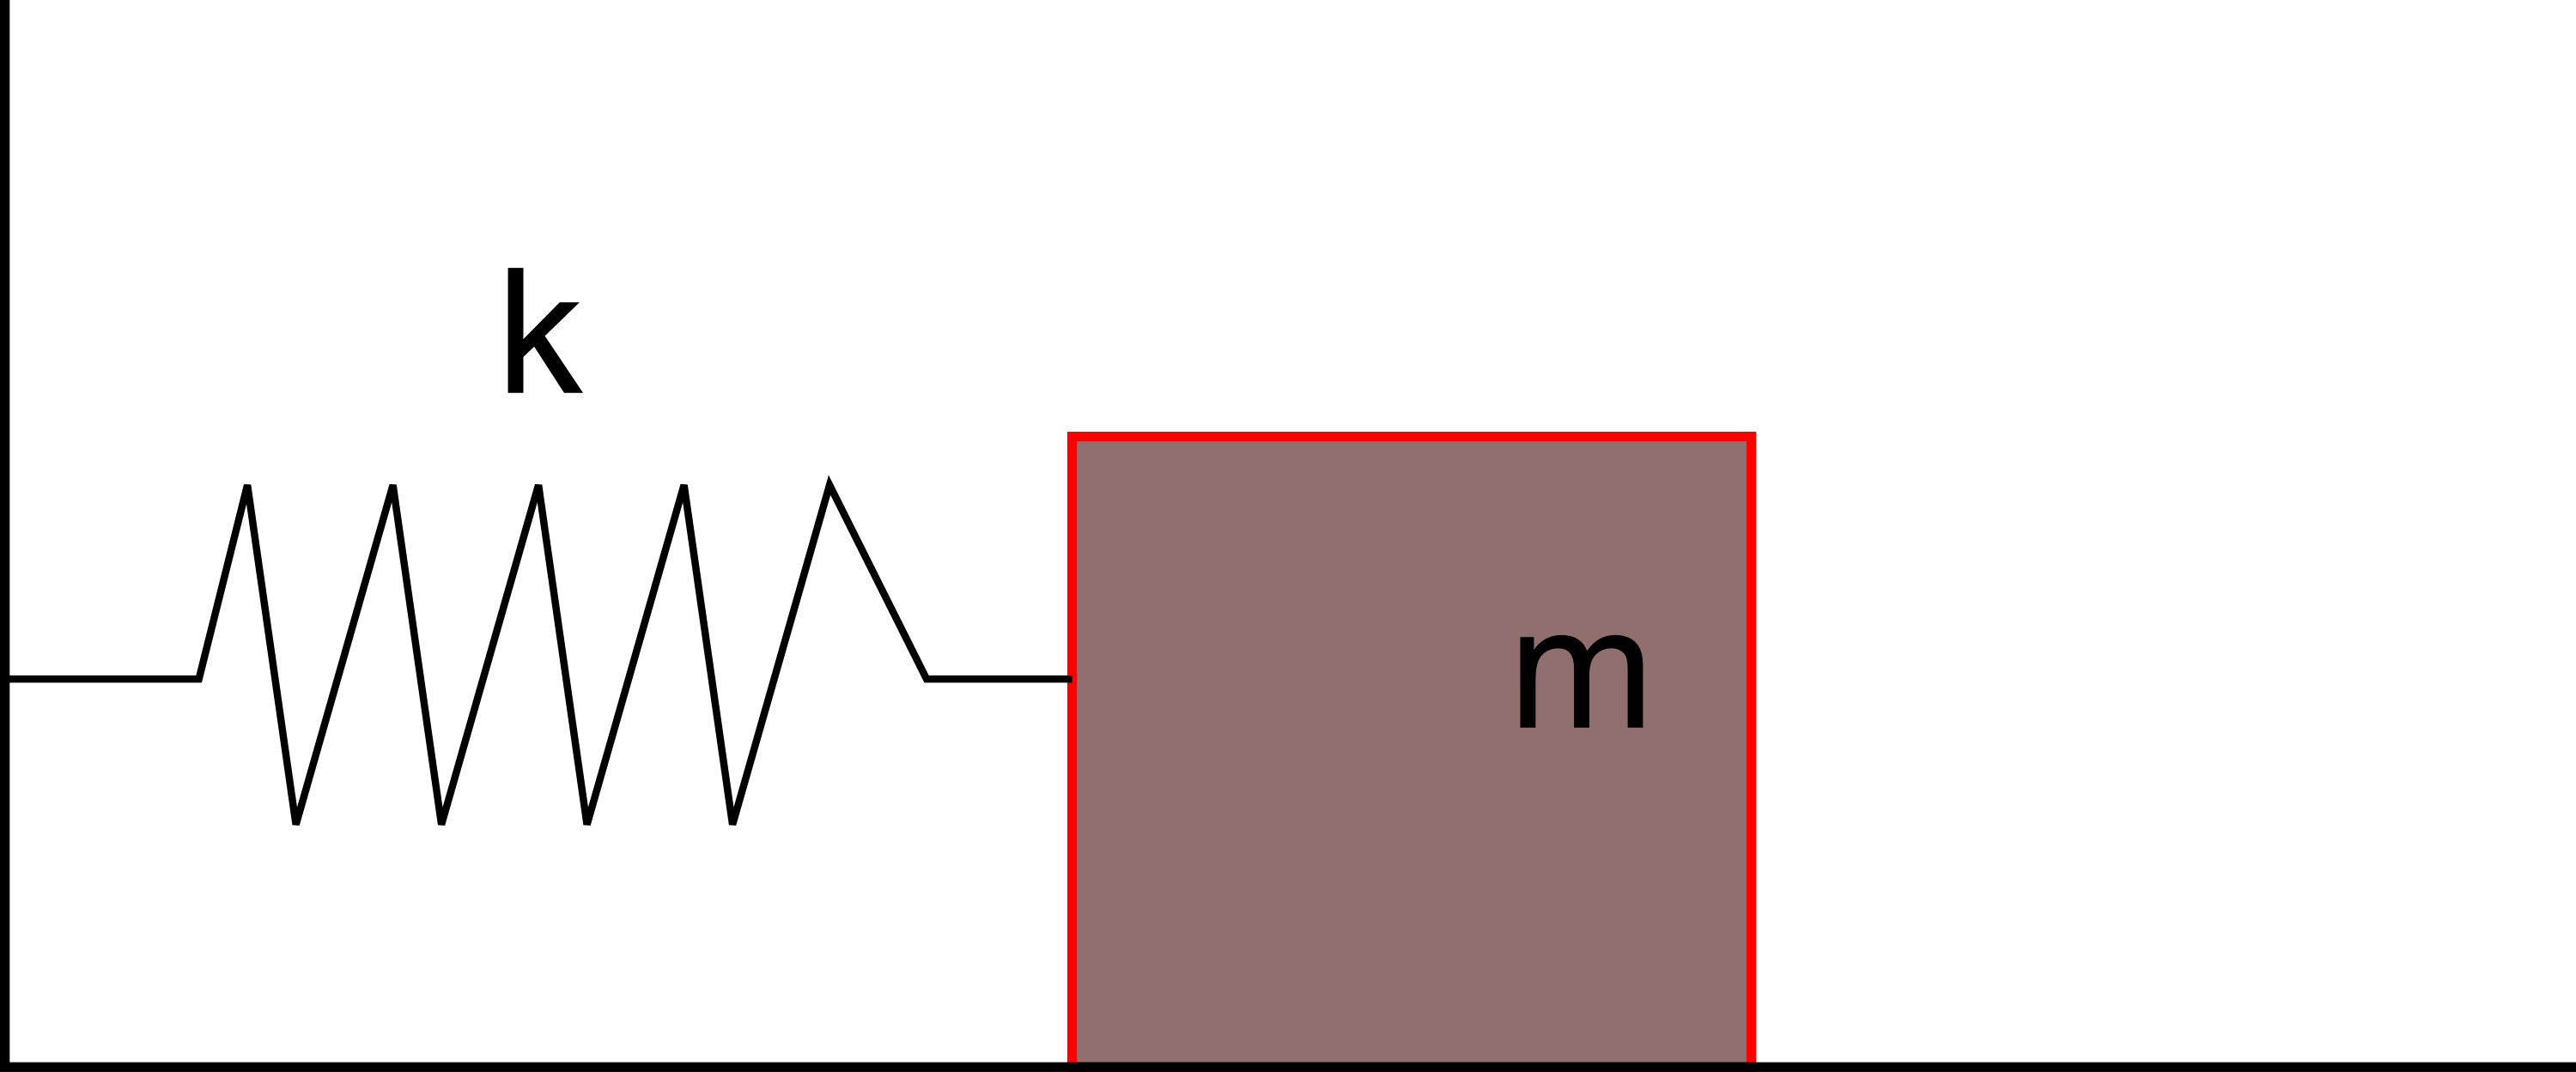
\includegraphics[width=6cm]{img/springMassStatic}

  Section 4.1 - Redux: The governing equation for a mass/spring system
  is
  \begin{eqnarray*}
    mx'' + bx'+kx & = & f(t).
  \end{eqnarray*}

  The constants $m$, $b$, and $k$ are all non-negative.

  The function $f(t)$ is called the \textit{forcing function}.

  This is a \underline{\textit{conceptual model}} for many physical systems.

\end{frame}


\begin{frame}
  \frametitle{Special Case}

  Suppose that we have a periodic forcing:
  \begin{eqnarray*}
    f(t) & = & F_0 \cos(\omega t), \\
    x(0) & = & 0, \\
    x'(0) & = & 0.
  \end{eqnarray*}

  Suppose that there is no friction, $b=0$,
  \begin{eqnarray*}
    m x'' + kx & = & F_0 \cos(\omega t).
  \end{eqnarray*}

  This is an idealized system used to gain insight into real physical
  systems. It allows us to ask \textit{``what if....?''}

\end{frame}


\begin{frame}
  \frametitle{Homogeneous and Particular Solution}

  \begin{eqnarray*}
    x_h & = & C_1 \cos\lp\sqrt{\frac{k}{m}}t\rp + C_2 \sin\lp\sqrt{\frac{k}{m}}t\rp.
  \end{eqnarray*}

  Assume that $\omega \neq \sqrt{\frac{k}{m}}$, then the particular
  solution is
  \begin{eqnarray*}
    x_p & = & \frac{F_0}{m\lp\frac{k}{m}-\omega^2\rp} \cos(\omega t).
  \end{eqnarray*}

  \uncover<2->{You should be able to show this on your own using ideas we have already covered in class.}

\end{frame}


\begin{frame}
  \frametitle{Solve for the Constants}

  \begin{eqnarray*}
    x & = & C_1 \cos\lp\sqrt{\frac{k}{m}}t\rp + C_2 \sin\lp\sqrt{\frac{k}{m}}t\rp+ 
           \frac{F_0}{m\lp\frac{k}{m}-\omega^2\rp} \cos(\omega t).
  \end{eqnarray*}

  The initial conditions yield
  \begin{eqnarray*}
    x(0) & = & C_1 + \frac{F_0}{m\lp\frac{k}{m}-\omega^2\rp} \\
    \Rightarrow C_1 & = & \frac{-F_0}{m\lp\frac{k}{m}-\omega^2\rp}
  \end{eqnarray*}

\end{frame}


\begin{frame}
  \frametitle{Satisfy the Velocity}

  \begin{eqnarray*}
    x' & = & - C_1 \sqrt{\frac{k}{m}} \sin\lp\sqrt{\frac{k}{m}}t\rp + C_2 \sqrt{\frac{k}{m}} \cos\lp\sqrt{\frac{k}{m}}t\rp \\ 
    & & - \frac{\omega F_0}{m\lp\frac{k}{m}-\omega^2\rp} \sin(\omega t), \\
    \Rightarrow C_2 & = & 0.
  \end{eqnarray*}

  \uncover<2->
  {
    The solution is 
    \redText{
      \begin{eqnarray*}
        x & = & \frac{-F_0}{m\lp\frac{k}{m}-\omega^2\rp} \cos\lp\sqrt{\frac{k}{m}}t\rp 
        + \frac{F_0}{m\lp\frac{k}{m}-\omega^2\rp} \cos(\omega t).
      \end{eqnarray*}
    }
  }


\end{frame}


\begin{frame}
  \frametitle{Obvious Trigonometric Identity}

  As we \textbf{all} know
  \begin{eqnarray*}
    \cos(u) - \cos(v) & = & -2 \sin\lp\frac{u-v}{2}\rp \sin\lp\frac{u+v}{2}\rp.
  \end{eqnarray*}

  Our solution can be written in the form
  \begin{eqnarray*}
    x(t) & = & \frac{-F_0}{m\lp\frac{k}{m}-\omega^2\rp} \sin\lp\lp\omega-\sqrt{\frac{k}{m}}\rp t\rp
                                                        \sin\lp\lp\omega+\sqrt{\frac{k}{m}}\rp t\rp
  \end{eqnarray*}

  Plots of the function are given on pages 262-267 in your book.

\end{frame}

\subsection{Example}

\iftoggle{clicker}{%
\begin{frame}
  \frametitle{Clicker Quiz}

      \ifnum\value{clickerQuiz}=1{%

        \vfill

        Determine the homogeneous solution to the differential equation
        \begin{eqnarray*}
          2 x'' + 10 x & = & 3 \cos(2t)
        \end{eqnarray*}


        \vfill

        \begin{tabular}{ll}
          A: & $x=C_1\cos(5t) + C_2\sin(5t)$ \\
          B: & $x=C_1\cos(\sqrt{5}t) + C_2\sin(\sqrt{5}t)$ \\
          C: & $x=C_1e^{5t} + C_2 t e^{5t}$ \\
          D: & $x=C_1e^{\sqrt{5t}} + C_2 t e^{\sqrt{5}t}$ \\
        \end{tabular}


        \vfill

      }\fi

      \ifnum\value{clickerQuiz}=2{%

        \vfill

        Determine the homogeneous solution to the differential equation
        \begin{eqnarray*}
          2 x'' + 10 x & = & 3 \cos(2t)
        \end{eqnarray*}


        \vfill

        \begin{tabular}{ll}
          A: & $x=C_1e^{5t} + C_2 t e^{5t}$ \\
          B: & $x=C_1e^{\sqrt{5t}} + C_2 t e^{\sqrt{5}t}$ \\
          C: & $x=C_1\cos(5t) + C_2\sin(5t)$ \\
          D: & $x=C_1\cos(\sqrt{5}t) + C_2\sin(\sqrt{5}t)$ \\
        \end{tabular}


        \vfill

     }\fi
   
     \ifnum\value{clickerQuiz}=3{%
         Determine the homogeneous solution to the differential equation
        \begin{eqnarray*}
          2 x'' + 10 x & = & 3 \cos(2t)
        \end{eqnarray*}


        \vfill

        \begin{tabular}{ll}
          A: & $x=C_1e^{5t} + C_2 t e^{5t}$ \\
          B: & $x=C_1e^{\sqrt{5t}} + C_2 t e^{\sqrt{5}t}$ \\
          C: & $x=C_1\cos(5t) + C_2\sin(5t)$ \\
          D: & $x=C_1\cos(\sqrt{5}t) + C_2\sin(\sqrt{5}t)$ \\
        \end{tabular}

        \vfill

    }\fi
  

\end{frame}
}


\begin{frame}                   
  \frametitle{The problem}      
                                
  A two kilogram mass is attached to a spring with constant ten N/m on
  a horizontal table. The mass is driven with a periodic force of
  \begin{eqnarray*}
    f(t) & = & 3 \cos(2t).
  \end{eqnarray*}
  the system is started from rest at the equilibrium point.

  Governing equation:
  \begin{eqnarray*}
    2 x'' + 10 x & = & 3 \cos(2t)
  \end{eqnarray*}

\end{frame}


\begin{frame}
  \frametitle{Solution}

  \begin{eqnarray*}
    2 x'' + 10 x & = & 3 \cos(2t), \\
    x(0) & = & 0, \\
    x'(0) & = & 0.
  \end{eqnarray*}

  The solution is 
  \begin{eqnarray*}
    x(t) & = & -\frac{3}{2}\cos(\sqrt{5} t) + \frac{3}{2} \sin( 2 t), \\
         & = & \frac{3}{2} \left[ -\cos(\sqrt{5} t) + \sin( 2 t) \right], \\
         \only<1>{%
           & = & 3 \sin\lp\frac{2-\sqrt{5}}{2}t\rp \sin\lp\frac{2+\sqrt{5}}{2} t\rp.\\
         }
         \only<2->{%
           & = & 3 \sin\lp\underbrace{\frac{2-\sqrt{5}}{2}}_{\mathrm{long~wave}}t\rp 
                   \sin\lp\underbrace{\frac{2+\sqrt{5}}{2}}_{\mathrm{short~wave}} t\rp.
         }
  \end{eqnarray*}

\end{frame}

\begin{frame}
  \frametitle{Plots}

  \only<1>{\centerline{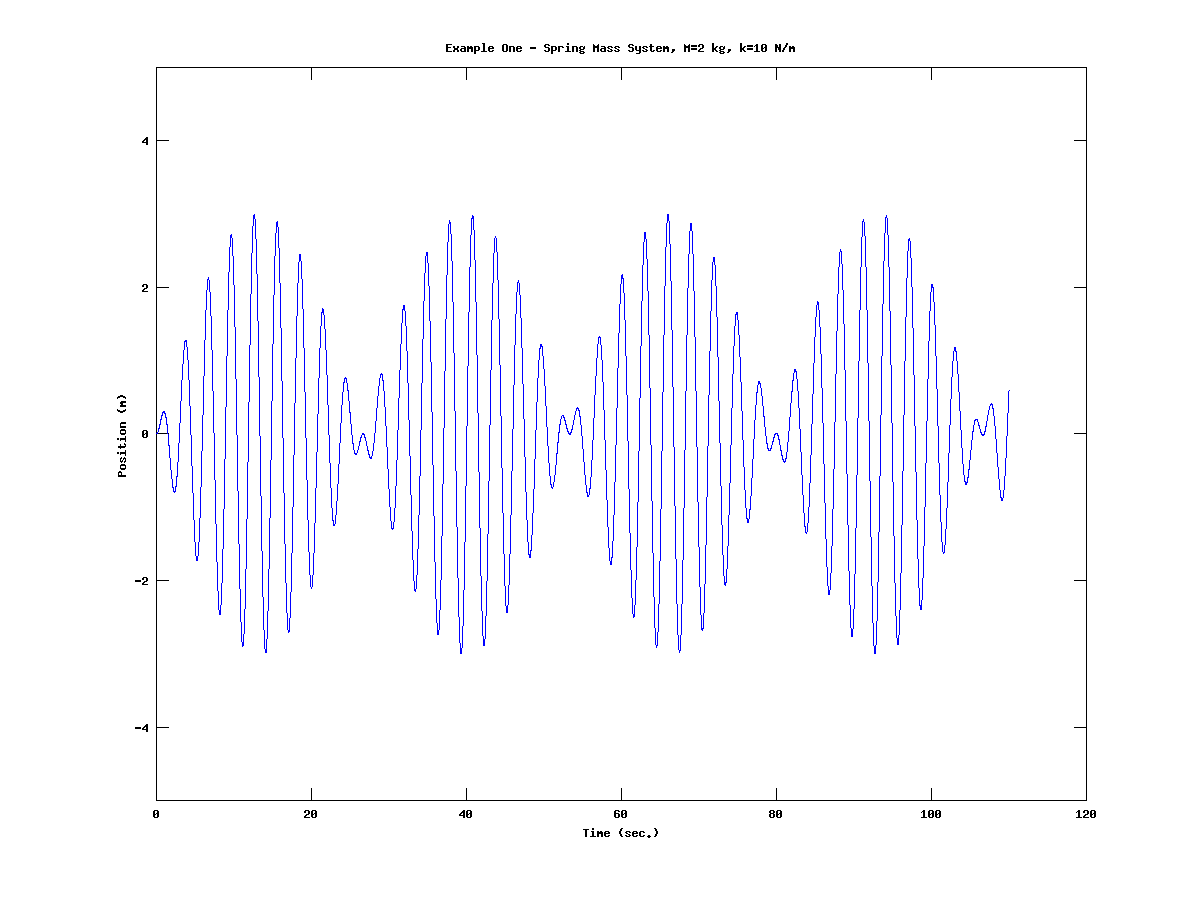
\includegraphics[width=11cm]{img/beats}}}
  \only<2>{\centerline{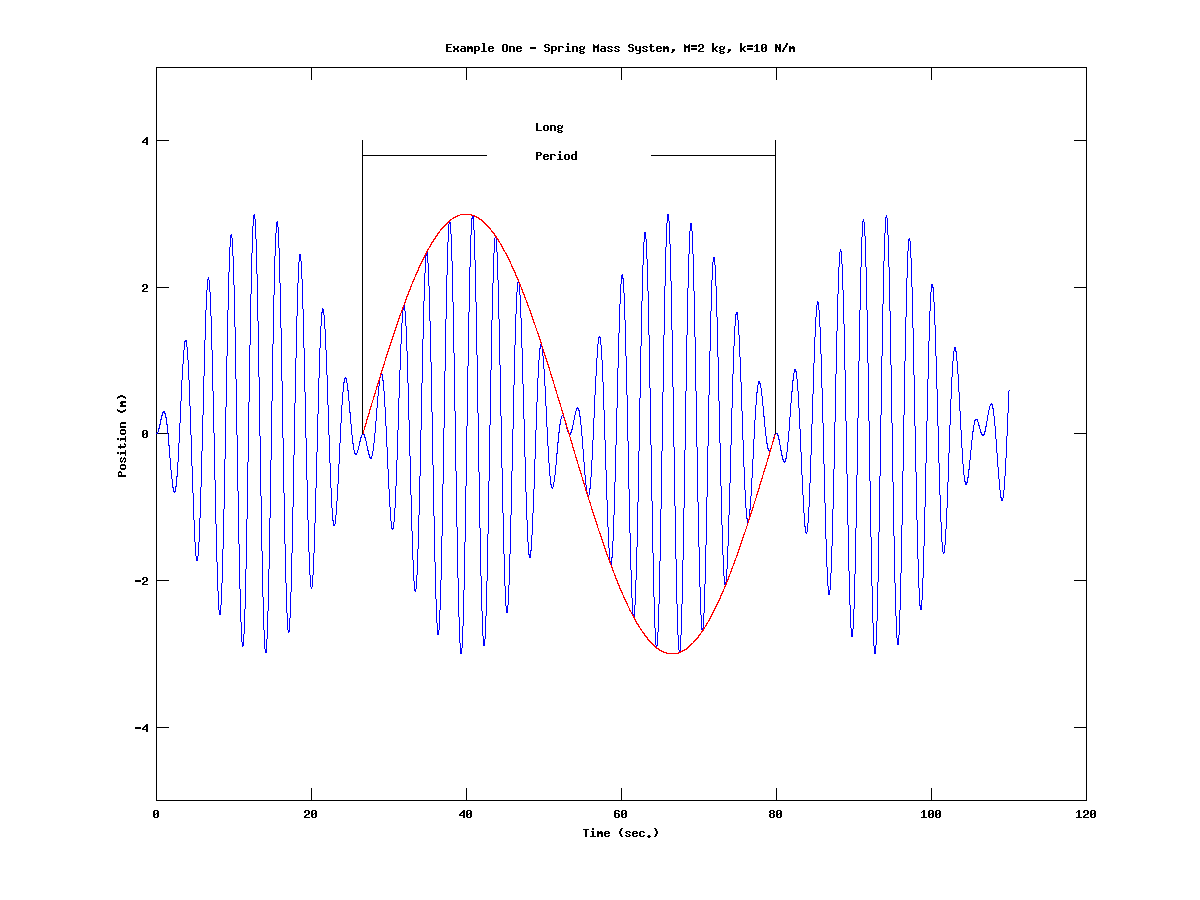
\includegraphics[width=11cm]{img/beatsLong}}}
  \only<3>{\centerline{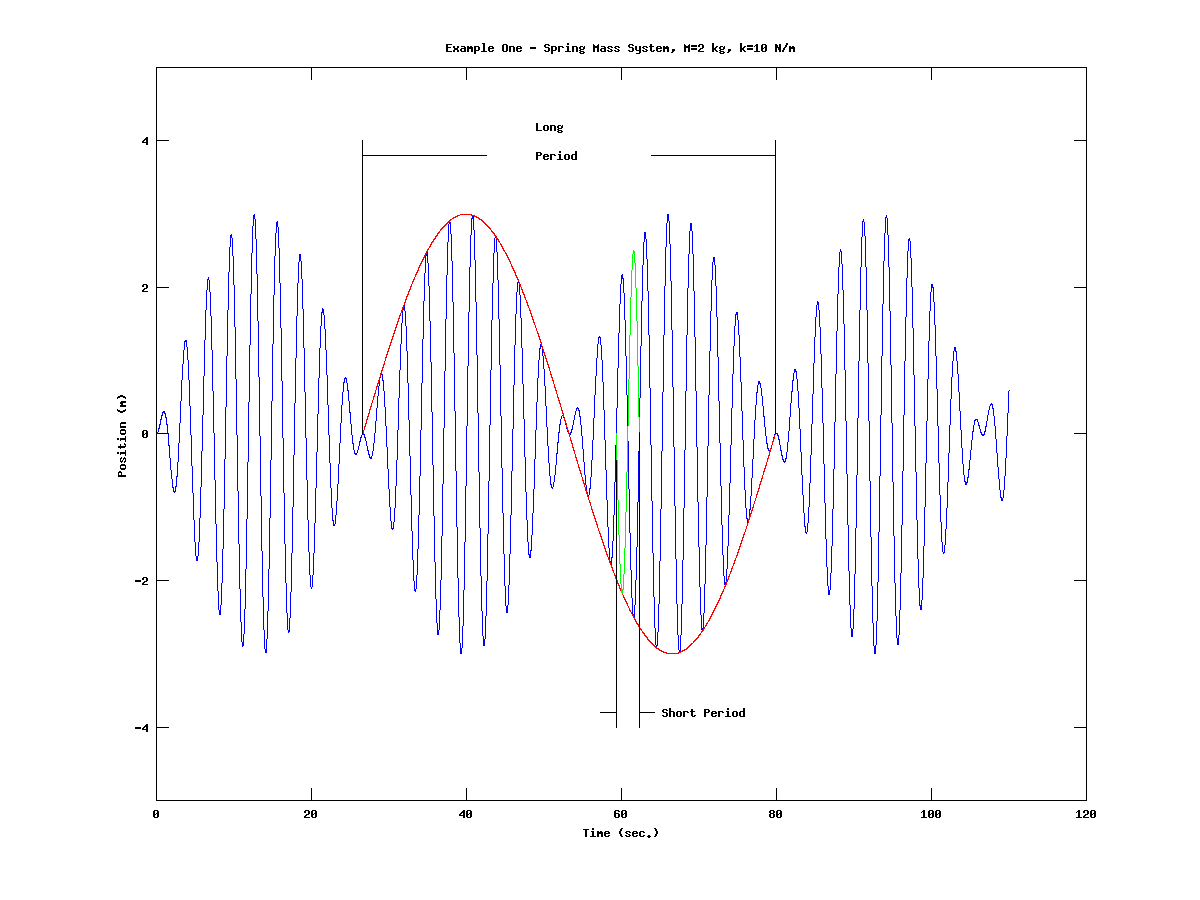
\includegraphics[width=11cm]{img/beatsShort}}}


\end{frame}



\begin{frame}
  \frametitle{The problem}      
                                
  A two kilogram mass is attached to a spring with constant ten N/m on
  a horizontal table. The mass is driven with a periodic force of
  \begin{eqnarray*}
    f(t) & = & 3 \cos(\sqrt{5} t).
  \end{eqnarray*}
  the system is started from rest at the equilibrium point.

  Governing equation:
  \begin{eqnarray*}
    2 x'' + 10 x & = & 3 \cos(\sqrt{5} t)
  \end{eqnarray*}

\end{frame}


\begin{frame}
  \frametitle{Solution}

  \begin{eqnarray*}
    2 x'' + 10 x & = & 3 \cos(\sqrt{5} t), \\
    x(0) & = & 0, \\
    x'(0) & = & 0.
  \end{eqnarray*}

  The homogeneous solution is 
  \begin{eqnarray*}
    x_h & = & C_1 \cos(\sqrt{5} t) + C_2 \sin(\sqrt{5} t).
  \end{eqnarray*}

  \only<2->
  {
    Guess a particular solution,
    \begin{eqnarray*}
      x_p & = & A t \cos(\sqrt{5} t) + B t \sin(\sqrt{5} t).
    \end{eqnarray*}
  }

\end{frame}

\begin{frame}
  \frametitle{The Solution}

  \begin{eqnarray*}
    x(t) & = & C_1 \cos(\sqrt{5}t) + C_2\sin(\sqrt{5} t) + \frac{3}{4\sqrt{5}} t \sin(\sqrt{5}t), \\
         & = & \frac{3}{4\sqrt{5}} t \sin(\sqrt{5}t).
  \end{eqnarray*}

  \only<2>{\centerline{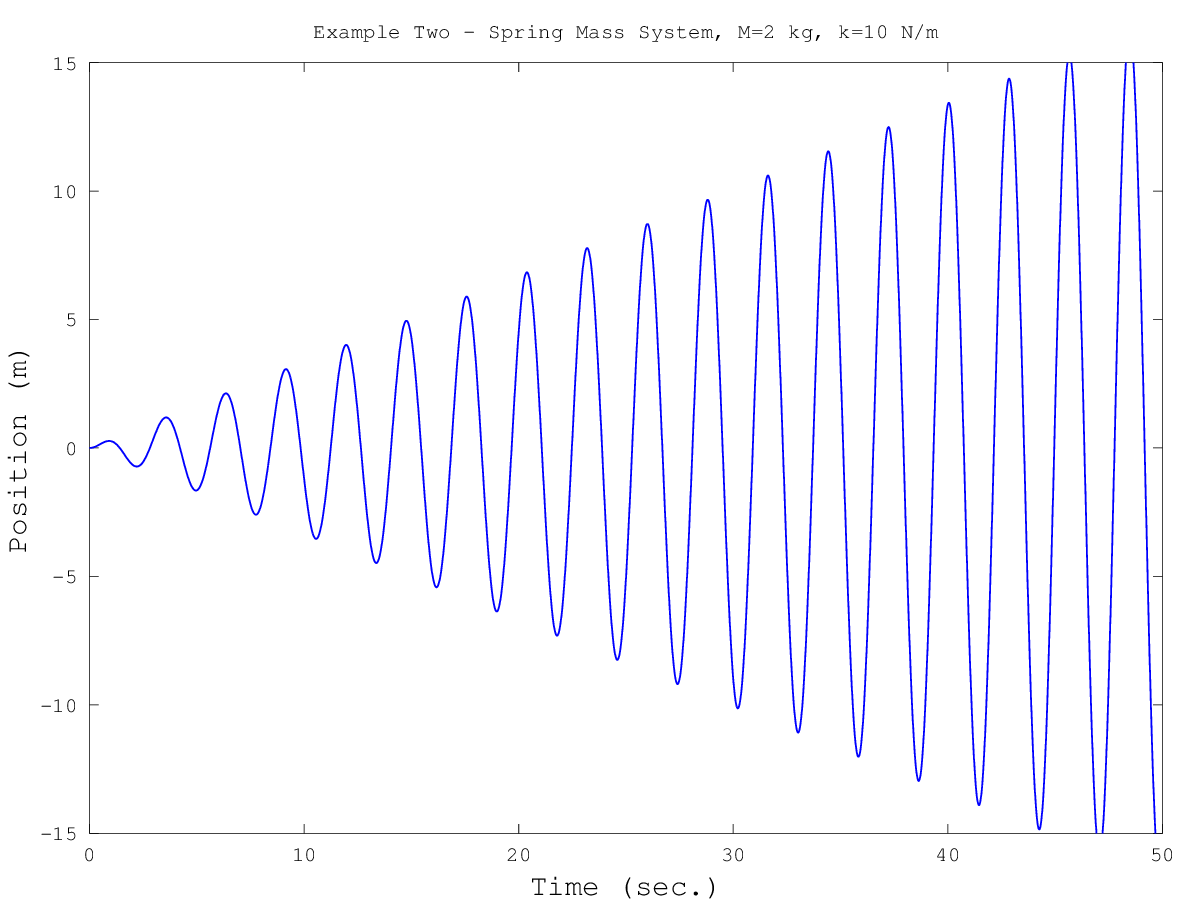
\includegraphics[width=5cm]{img/resonance}}}
  \only<3>{\centerline{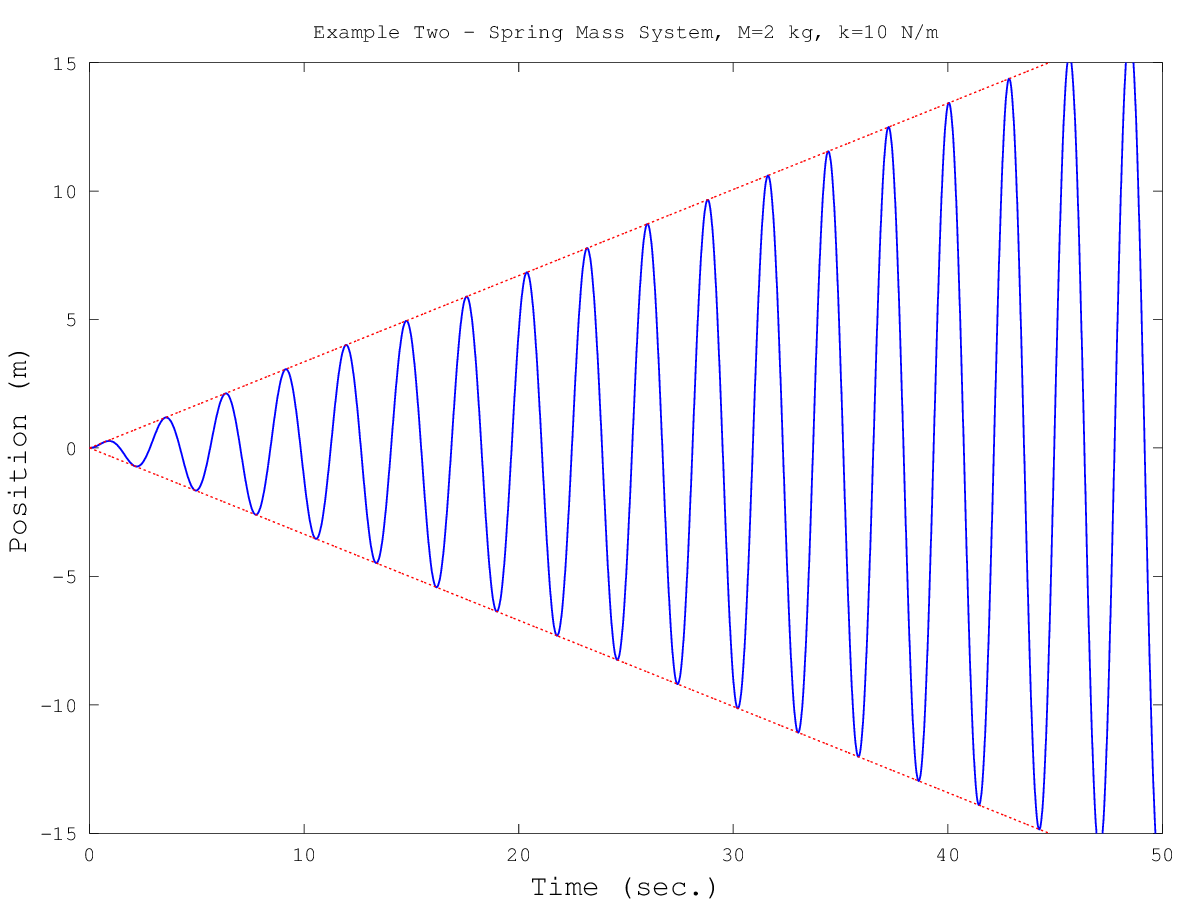
\includegraphics[width=5cm]{img/resonanceBounds}}}

\end{frame}


% LocalWords:  Clarkson pausesection hideothersubsections




% %%%%%%%%%%%%%%%%%%%%%%%%%%%%%%%%%%%%%%%%%%%%%%%%%%%%%%%%%%%%
% Back to eigen values and linear algebrea

\part{Eigen-Vectors/Values}
\lecture{EigenVectors/Values}{Eigen-Vectors/Values}
\section{Eigenvalues and Eigenvectors}


\title{Ordinary Differential Equations}
\subtitle{Math 232 - Eigenvalues and eigenvectors}
\date{30 October 2013}

\begin{frame}
  \titlepage
\end{frame}

\begin{frame}
  \frametitle{Outline}
  \tableofcontents[currentsection]
\end{frame}


\subsection{Eigenvalues and Eigenvectors}


\begin{frame}
  \frametitle{Eigenvalues and Eigenvectors}

  Suppose that we have a system of differential equations,
  \begin{eqnarray*}
    \frac{d}{dt} \vec{x} & = & A \vec{x}.
  \end{eqnarray*}
  Assume that $A$ is a square matrix.

  What if we can find a vector, $\vec{v}$, that satisfies
  \begin{eqnarray*}
    A \vec{v} & = & \lambda \vec{v},
  \end{eqnarray*}
  where $\lambda$ is a scalar (number)?

\end{frame}


\begin{frame}
  If so. then....
  \begin{eqnarray*}
    \frac{d}{dt} \vec{v} & = & A \vec{v}, \\
    & = & \lambda \vec{v}.
  \end{eqnarray*}

  \only<1>%
  {
    But,
    \begin{eqnarray*}
      \vec{v} & = & 
      \left[
        \begin{array}{r}
          x_1 \\ x_2 \\ x_3 \\ \vdots \\ x_n
        \end{array}
      \right].
    \end{eqnarray*}
  }
  
  \only<2>%
  {
    This implies that
    \begin{eqnarray*}
      \deriv{x_1}{t} & = & \lambda x_1, \\
      \deriv{x_2}{t} & = & \lambda x_2, \\
      \deriv{x_3}{t} & = & \lambda x_3, \\
      \vdots         &   & \vdots \\
      \deriv{x_n}{t} & = & \lambda x_n
    \end{eqnarray*}

    We can solve each one of these equations separately!
  }

\end{frame}


\begin{frame}
  \frametitle{Eigenvalues and Eigenvectors}

  \begin{definition}
    Given a square matrix, $A$, an \blueText{eigenvector}, $\vec{v}$,
    and an associated \blueText{eigenvalue}, $\lambda$, satisfy
    \begin{eqnarray*}
      A \vec{v} & = & \lambda \vec{v}.
    \end{eqnarray*}
  \end{definition}



\end{frame}


\iftoggle{clicker}{%
\begin{frame}
  \frametitle{Clicker Quiz}

      \ifnum\value{clickerQuiz}=1{%
        We want to solve a system of linear equations
        \begin{eqnarray*}
          A \vec{x} & = & \vec{b}.
        \end{eqnarray*}
        We find the determinant of the matrix $A$, and the determinant is zero. 

        What does this imply about the solutions to the linear system.
        \vfill

        \begin{tabular}{ll}
          A: & The solution is unique. \\
          B: & There are infinite solutions. \\
          C: & There are no solutions. \\
          D: & Either B or C. \\
        \end{tabular}
        \vfill

      }\fi

      \ifnum\value{clickerQuiz}=2{%
        We want to solve a system of linear equations
        \begin{eqnarray*}
          A \vec{x} & = & \vec{b}.
        \end{eqnarray*}
        We find the determinant of the matrix $A$, and the determinant is zero. 

        What does this imply about the solutions to the linear system.
        \vfill

        \begin{tabular}{ll}
          A: & The solution is unique. \\
          B: & There are infinite solutions. \\
          C: & There are no solutions. \\
          D: & Either B or C. \\
        \end{tabular}

        \vfill

     }\fi
   
     \ifnum\value{clickerQuiz}=3{%
        \vfill
        We want to solve a system of linear equations
        \begin{eqnarray*}
          A \vec{x} & = & \vec{b}.
        \end{eqnarray*}
        We find the determinant of the matrix $A$, and the determinant is zero.

        What does this imply about the solutions to the linear system.
        \vfill

        \begin{tabular}{ll}
          A: & The solution is unique. \\
          B: & There are infinitely many solutions. \\
          C: & There are no solutions. \\
          D: & Either B or C. \\
        \end{tabular}

    }\fi
  

\end{frame}
}



\begin{frame}
  \frametitle{How to find}

  Given $A$ how can we find its eigenvalues and eigenvectors?
  \begin{eqnarray*}
    A \vec{v} & = & \lambda \vec{v}, \\
    A \vec{v} - \lambda \vec{v} & = & 0, \\
    A \vec{v} - \lambda \redText{I} \vec{v} & = & 0, \\
    \lp A - \lambda I \rp \vec{v} & = & 0.
  \end{eqnarray*}

  \only<1>{\textit{Remember $\vec{v}$ is a vector and $A$ is an array. We cannot
    add them!}}

  \uncover<2->{\redText{One solution is $\vec{v}=\vec{0}$.}} 
  \uncover<3->{\blueText{We do not like this solution.}}
  \uncover<4->{We must have a situation where there is not a unique solution. If there
    is not a unique solution then this implies that
  \begin{eqnarray*}
    \det\lp A - \lambda I \rp & = & 0.
  \end{eqnarray*}
  Find a value for $\lambda$ that makes this true. (\redText{Note that there
  will be infinitely many solutions for $\vec{v}$.})}

\end{frame}


\begin{frame}
  \frametitle{Finding Eigenvalues and Eigenvectors}

  Given a square matrix, $A$, to find the eigenvalues and eigenvectors do the following:
  \begin{enumerate}
  \item Determine the characteristic equation:
    \begin{eqnarray*}
      \det\lp A - \lambda I \rp & = & 0.
    \end{eqnarray*}
  \item Solve the equation for the \blueText{values} of $\lambda$,
    call them $\lambda_j$.
  \item Find the eigenvector associated with each value of $\lambda_j$,
    \begin{eqnarray*}
      \lp A - \lambda_j I \rp \vec{v}_j & = & \vec{0}.
    \end{eqnarray*}
    (Note that there will be infinitely many solutions for each
    $\vec{v}_j$.) Solving linear systems means dealing with
    RREF. Woohoo!!
  \end{enumerate}

\end{frame}

\subsection{Examples}

\begin{frame}
  \frametitle{Example}

  \begin{eqnarray*}
    A & = & \arrayTwo{12}{-10}{15}{-13}.
  \end{eqnarray*}

  \uncover<2->
  {
    Find the characteristic equation:
    \begin{eqnarray*}
      \det\lp\arrayTwo{12-\lambda}{-10}{15}{-13-\lambda}\rp & = & \lambda^2+\lambda-6.
    \end{eqnarray*}

    Find the values of $\lambda$:
    \begin{eqnarray*}
      \lambda^2+\lambda-6 & = & (\lambda-2)(\lambda+3), \\
      & = & 0.
    \end{eqnarray*}
    So \redText{$\lambda_1 = 2$} and \redText{$\lambda_2=-3$}.
  }

\end{frame}


\begin{frame}
  Find the vectors:

  $\lambda_1 = 2$:
  \begin{eqnarray*}
    \arrayTwo{10}{-10}{15}{-15} \vecTwo{x}{y} & = & \vecTwo{0}{0}, \\
    10x - 10y & = & 0, \\
    15x - 15y & = & 0, \\
    x & = & y.
  \end{eqnarray*}

  The first eigenvector is 
  \begin{eqnarray*}
    \vec{v}_1 & = & \vecTwo{y}{y}, \\
    & = & y \vecTwo{1}{1}.
  \end{eqnarray*}

  \redText{Let}
  \begin{eqnarray*}
    \redText{\vec{v}_1} & \redText{=} & \redText{\vecTwo{1}{1}}.
  \end{eqnarray*}

\end{frame}

\begin{frame}
  Find the vectors:

  $\lambda_2 = -3$:
  \begin{eqnarray*}
    \arrayTwo{15}{-10}{15}{-10} \vecTwo{x}{y} & = & \vecTwo{0}{0}, \\
    15x - 10y & = & 0, \\
    15x - 10y & = & 0, \\
    x & = & \frac{2}{3} y.
  \end{eqnarray*}

  The second eigenvector is 
  \begin{eqnarray*}
    \vec{v}_2 & = & \vecTwo{\frac{2}{3}y}{y}, \\
    & = & y \vecTwo{\frac{2}{3}}{1}.
  \end{eqnarray*}

  \redText{Let}
  \begin{eqnarray*}
    \redText{\vec{v}_2} & \redText{=} & \redText{\vecTwo{2}{3}}.
  \end{eqnarray*}

\end{frame}






\begin{frame}
  \frametitle{Example}

  \begin{eqnarray*}
    A & = & \arrayTwo{4}{18}{-3}{-11}.
  \end{eqnarray*}

  \uncover<2->
  {
    Find the characteristic equation:
    \begin{eqnarray*}
      \det\lp\arrayTwo{4-\lambda}{18}{-3}{-11-\lambda}\rp & = & \lambda^2+7\lambda+10.
    \end{eqnarray*}
    
    Find the values of $\lambda$:
    \begin{eqnarray*}
      \lambda^2+7\lambda+10 & = & (\lambda+2)(\lambda+5), \\
      & = & 0.
    \end{eqnarray*}
    So \redText{$\lambda_1 = -2$} and \redText{$\lambda_2=-5$}.
  }

\end{frame}


\begin{frame}
  Find the vectors:

  $\lambda_1 = -2$:
  \begin{eqnarray*}
    \arrayTwo{6}{18}{-3}{-9} \vecTwo{x}{y} & = & \vecTwo{0}{0}, \\
    6x + 18y & = & 0, \\
    -3x - 9y & = & 0, \\
    x & = & -3y.
  \end{eqnarray*}

  The first eigenvector is 
  \begin{eqnarray*}
    \vec{v}_1 & = & \vecTwo{-3y}{y}, \\
    & = & y \vecTwo{-3}{1}.
  \end{eqnarray*}

  \redText{Let}
  \begin{eqnarray*}
    \redText{\vec{v}_1} & \redText{=} & \redText{\vecTwo{-3}{1}}.
  \end{eqnarray*}

\end{frame}

\begin{frame}
  Find the vectors:

  $\lambda_2 = -5$:
  \begin{eqnarray*}
    \arrayTwo{9}{18}{-3}{-6} \vecTwo{x}{y} & = & \vecTwo{0}{0}, \\
    9x + 18y & = & 0, \\
    -3x - 6y & = & 0, \\
    x & = & -2 y.
  \end{eqnarray*}

  The second eigenvector is 
  \begin{eqnarray*}
    \vec{v}_2 & = & \vecTwo{-2y}{y}, \\
    & = & y \vecTwo{-2}{1}.
  \end{eqnarray*}

  \redText{Let}
  \begin{eqnarray*}
    \redText{\vec{v}_2} & \redText{=} & \redText{\vecTwo{-2}{1}}.
  \end{eqnarray*}

\end{frame}



\begin{frame}
  \frametitle{Theorem - Distinct Eigenvalues Makes Life Easier}

  \begin{theorem}
    If the eigenvalues of an $n\times n$ matrix include \blueText{\textbf{$n$}}
    \blueText{distinct} values then the eigenvectors are linearly
    independent.
  \end{theorem}


  \vfill

  \uncover<2->
  {
    So what? When we start solving DEs it will mean we are essentially
    done. 
  }

  \vfill

\end{frame}



\begin{frame}
  \frametitle{Example}

  See example 5 on page 318.
  \begin{eqnarray*}
    A & = & \arrayThree{-2}{1}{1}{1}{-2}{1}{1}{1}{-2}.
  \end{eqnarray*}

  \uncover<2->
  {
    Find the characteristic equation:
    \begin{eqnarray*}
      \det\lp\arrayThree{-2-\lambda}{1}{1}{1}{-2-\lambda}{1}{1}{1}{-2-\lambda}\rp
      & = & \lambda (\lambda+3)^2.
    \end{eqnarray*}

    Find the values of $\lambda$:
    \begin{eqnarray*}
      \lambda (\lambda+3)^2 & = & 0.
    \end{eqnarray*}
    So \redText{$\lambda_1 = 0$} and \redText{$\lambda_2=-3$}.
  }

\end{frame}



\begin{frame}
  Find the vectors:

  $\lambda_1 = 0$:
  \begin{eqnarray*}
    \arrayThree{-2}{1}{1}{1}{-2}{1}{1}{1}{-2}\vecThree{x}{y}{z} & = & \vecThree{0}{0}{0}, \\
  \end{eqnarray*}

  Express this system in an augmented matrix and put it in reduced row
  echelon form:
  \begin{eqnarray*}
    \mathrm{RREF}\startRowFour
    \oneRowFour{-2}{1}{1}{0} 
    \oneRowFour{1}{-2}{1}{0}
    \oneRowFour{1}{1}{-2}{0}
    \stopRowOps
    & = & 
    \startRowFour
    \oneRowFour{1}{0}{-1}{0} 
    \oneRowFour{0}{1}{-1}{0}
    \oneRowFour{0}{0}{0}{0}
    \stopRowOps
  \end{eqnarray*}


\end{frame}

\begin{frame}
  The first eigenvector is 
  \begin{eqnarray*}
    \vec{v}_1 & = & \vecThree{z}{z}{z}, \\
    & = & z \vecThree{1}{1}{1}.
  \end{eqnarray*}

  Let
  \begin{eqnarray*}
    \vec{v}_1 & = & \vecThree{1}{1}{1}.
  \end{eqnarray*}

\end{frame}

\begin{frame}
  Find the vectors:

  $\lambda_2 = -3$:
  \begin{eqnarray*}
    \arrayThree{1}{1}{1}{1}{1}{1}{1}{1}{1}
    \vecThree{x}{y}{z} & = & \vecThree{0}{0}{0}, \\
  \end{eqnarray*}

  Express this system in an augmented matrix and put it in reduced row
  echelon form:
  \begin{eqnarray*}
    \mathrm{RREF}\startRowFour
    \oneRowFour{1}{1}{1}{0} 
    \oneRowFour{1}{1}{1}{0}
    \oneRowFour{1}{1}{1}{0}
    \stopRowOps
    & = & 
    \startRowFour
    \oneRowFour{1}{1}{1}{0} 
    \oneRowFour{0}{0}{0}{0}
    \oneRowFour{0}{0}{0}{0}
    \stopRowOps
  \end{eqnarray*}

\end{frame}

\begin{frame}

  The second eigenvector is 
  \begin{eqnarray*}
    \vec{v}_2 & = & \vecThree{-y-z}{y}{z}, \\
    & = & y \vecThree{-1}{1}{0} + z \vecThree{-1}{0}{1}.
  \end{eqnarray*}

  Let
  \begin{eqnarray*}
    \vec{v}_2 & = & \vecThree{-1}{1}{0}, \\
    \vec{v}_3 & = & \vecThree{-1}{0}{1}.
  \end{eqnarray*}

\end{frame}

\begin{frame}
  \frametitle{Example}

  \begin{eqnarray*}
    A & = & \arrayThree{2}{1}{1}{0}{1}{1}{0}{0}{1}.
  \end{eqnarray*}

  \uncover<2->
  {
    Find the characteristic equation:
    \begin{eqnarray*}
      \det\lp\arrayThree{2-\lambda}{1}{1}{0}{1-\lambda}{1}{0}{0}{1-\lambda}\rp
      & = & (2-\lambda) (1-\lambda)^2.
    \end{eqnarray*}

    Find the values of $\lambda$:
    \begin{eqnarray*}
      (2-\lambda) (1-\lambda)^2 & = & 0.
    \end{eqnarray*}
    So \redText{$\lambda_1 = 2$} and \redText{$\lambda_2=1$}.
  }

\end{frame}


\begin{frame}
  Find the vectors:

  $\lambda_1 = 2$:
  \begin{eqnarray*}
    \arrayThree{0}{1}{1}{0}{-1}{1}{0}{0}{-1}\vecThree{x}{y}{z} & = & \vecThree{0}{0}{0}, \\
  \end{eqnarray*}

  Express this system in an augmented matrix and put it in reduced row
  echelon form:
  \begin{eqnarray*}
    \mathrm{RREF}\startRowFour
    \oneRowFour{0}{1}{1}{0} 
    \oneRowFour{0}{-1}{1}{0}
    \oneRowFour{0}{0}{-1}{0}
    \stopRowOps
    & = & 
    \startRowFour
    \oneRowFour{0}{1}{0}{0} 
    \oneRowFour{0}{0}{1}{0}
    \oneRowFour{0}{0}{0}{0}
    \stopRowOps
  \end{eqnarray*}


\end{frame}

\begin{frame}
  The first eigenvector is 
  \begin{eqnarray*}
    \vec{v}_1 & = & \vecThree{x}{0}{0}, \\
    & = & x \vecThree{1}{0}{0}.
  \end{eqnarray*}

  Let
  \begin{eqnarray*}
    \vec{v}_1 & = & \vecThree{1}{0}{0}.
  \end{eqnarray*}

\end{frame}

\begin{frame}
  Find the vectors:

  $\lambda_2 = 1$:
  \begin{eqnarray*}
    \arrayThree{1}{1}{1}{0}{0}{1}{0}{0}{0}
    \vecThree{x}{y}{z} & = & \vecThree{0}{0}{0}, \\
  \end{eqnarray*}

  Express this system in an augmented matrix and put it in reduced row
  echelon form:
  \begin{eqnarray*}
    \mathrm{RREF}\startRowFour
    \oneRowFour{1}{1}{1}{0} 
    \oneRowFour{0}{0}{1}{0}
    \oneRowFour{0}{0}{0}{0}
    \stopRowOps
    & = & 
    \startRowFour
    \oneRowFour{1}{1}{0}{0} 
    \oneRowFour{0}{0}{1}{0}
    \oneRowFour{0}{0}{0}{0}
    \stopRowOps
  \end{eqnarray*}

\end{frame}

\begin{frame}

  The second eigenvector is 
  \begin{eqnarray*}
    \vec{v}_2 & = & \vecThree{-y}{y}{0}, \\
    & = & y \vecThree{-1}{1}{0}.
  \end{eqnarray*}

  Let
  \begin{eqnarray*}
    \vec{v}_2 & = & \vecThree{-1}{1}{0}.
  \end{eqnarray*}

  There are only two eigenvectors! If we want to solve a system of
  differential equations we have a problem.

\end{frame}

\iftoggle{clicker}{%
\begin{frame}
  \frametitle{Clicker Quiz}
      \ifnum\value{clickerQuiz}=1{%
        We have two distinct eigenvalues for a $3 \times 3$
        matrix. What does this imply about the number of linearly
        independent eigenvectors?

        \vfill
  
        \begin{tabular}{ll}
          A: & There are  two. \\
          B: & There are three. \\
          C: & There could be two or three, but there is not enough information. \\
          D: & Wut? \\
        \end{tabular}

        \vfill
  
      }\fi

      \ifnum\value{clickerQuiz}=2{%
        We have two distinct eigenvalues for a $3 \times 3$
        matrix. What does this imply about the number of linearly
        independent eigenvectors?
  
        \vfill
  
        \begin{tabular}{ll}
          A: & There are  two. \\
          B: & There are three. \\
          C: & There could be two or three, but there is not enough information. \\
          D: & Wut? \\
        \end{tabular}

        \vfill

     }\fi
     \ifnum\value{clickerQuiz}=3{%
        \vfill
       We have two distinct eigenvalues for a $3 \times 3$
        matrix. What does this imply about the number of linearly
        independent eigenvectors?

        \vfill

        \begin{tabular}{ll}
          A: & There are  two. \\
          B: & There are three. \\
          C: & There could be two or three,
             but there is not enough information. \\
          D: & Have no idea.\\
       \end{tabular}

    }\fi
\end{frame}
}




% LocalWords:  Clarkson pausesection hideothersubsections Eigen eigen
%  LocalWords:  Eigenvectors eigenvector eigenvectors RREF

\part{Systems-of-DEs}
\lecture{Systems of DEs}{Systems-of-DEs}
\section{Systems of DEs}


\title{Ordinary Differential Equations}
\subtitle{Math 232 - Solving Systems of Differential Equations}
\date{1 November 2013}

\begin{frame}
  \titlepage
\end{frame}

\begin{frame}
  \frametitle{Outline}
  \tableofcontents[ currentsection ]
\end{frame}


\subsection{Systems of Differential Equations}


\begin{frame}
  \frametitle{Systems of Differential Equations}

  Conceptual Model: Coupled System \\
  \centerline{\includegraphics[width=7cm]{img/doubleSpringMass}}

  \begin{eqnarray*}
    \deriv{~}{t} \lp m_1 \vec{v_1} \rp & = & \sum_j \vec{F}_{1j} \\
    \deriv{~}{t} \lp m_2 \vec{v_2} \rp & = & \sum_k \vec{F}_{2k} 
  \end{eqnarray*}

  \uncover<2->{%
    These two equations depend on each other.
    }

\end{frame}


\begin{frame}
  \frametitle{Vicini Told Me to Go Back To The Beginning}

  \begin{eqnarray*}
    \deriv{~}{t} x_1  & = & a_{11} x_1 + a_{12} x_2 + f(t), \\
    \deriv{~}{t} x_2  & = & a_{21} x_1 + a_{22} x_2 + g(t).
  \end{eqnarray*}

  Writing the system in matrix/vector form we get
  \begin{eqnarray*}
    \deriv{~}{t} \vecTwo{x_1}{x_2} & = & 
    \arrayTwo{a_{11}}{a_{12}}{a_{21}}{a_{22}} \vecTwo{x_1}{x_2} + 
    \vecTwo{f(t)}{g(t)}.
  \end{eqnarray*}

\end{frame}


\begin{frame}
  \frametitle{More General Notation}

  \begin{eqnarray*}
    \deriv{~}{t} \vec{x}(t) & = & A(t) \vec{x}(t) + \vec{f}(t), \\
    \mathrm{or}~~\deriv{~}{t} \vec{x} & = & A \vec{x} + \vec{f}, \\
    \vec{x}(t_0) & = & \vec{c} 
  \end{eqnarray*}

  If $\vec{f}=\vec{0}$ then the system of equations is
  {\color{red}homogeneous}, otherwise, the system is
  {\color{red}nonhomogeneous}.

  {\color{blue}Remark:} 
  \begin{itemize}
  \item Solutions are the sum of homogeneous and particular solutions.
  \item Solutions are found by assuming a general form and then
    searching for the ``right answer.'' \textit{(Hint: exponential
      functions served us well in the past.)}
  \end{itemize}

\end{frame}

\subsection{Example}

\iftoggle{clicker}{%
\begin{frame}
  \frametitle{Clicker Quiz}

   \ifnum\value{clickerQuiz}=1{%

    \vfill
   \begin{eqnarray*}
     \deriv{~}{t} x_1 & = & 5  x_1 + 24 x_2 + 8 e^{-11t}, \\
     \deriv{~}{t} x_2 & = & -2 x_1 -  9 x_2 + 4 e^{-11t}.
   \end{eqnarray*}

   Written in matrix/vector form we get\\[12pt]

   \begin{tabular}{ll}
          A: &  $\deriv{~}{t} \vecTwo{x_1}{x_2}  =  
      \arrayTwo{5}{24}{-2}{-9} \vecTwo{x_1}{x_2}
      + \vecTwo{8e^{-11t}}{4e^{-11t}}.$
       \\[12pt]
          B: &  $\deriv{~}{t} \vecTwo{x_1}{x_2}  =  
      \arrayTwo{5}{-2}{24}{-9} \vecTwo{x_1}{x_2}
      + \vecTwo{8e^{-11t}}{4e^{-11t}}.$
       \\
    \end{tabular}

    \vfill

 }\fi

 \ifnum\value{clickerQuiz}=2{%
   \vfill

   \begin{eqnarray*}
     \deriv{~}{t} x_1 & = & 5  x_1 + 24 x_2 + 8 e^{-11t}, \\
     \deriv{~}{t} x_2 & = & -2 x_1 -  9 x_2 + 4 e^{-11t}.
   \end{eqnarray*}

   Written in matrix/vector form we get\\[12pt]

   \begin{tabular}{ll}
     A: &  $\deriv{~}{t} \vecTwo{x_1}{x_2}  =  
     \arrayTwo{5}{-2}{24}{-9} \vecTwo{x_1}{x_2}
     + \vecTwo{8e^{-11t}}{4e^{-11t}}.$
     \\ [12pt]
     B: &  $\deriv{~}{t} \vecTwo{x_1}{x_2}  =  
     \arrayTwo{5}{24}{-2}{-9} \vecTwo{x_1}{x_2}
     + \vecTwo{8e^{-11t}}{4e^{-11t}}.$
     \\
   \end{tabular}

   \vfill

 }\fi

 \ifnum\value{clickerQuiz}=3{%
  \begin{eqnarray*}
    \deriv{~}{t} x_1 & = & 5  x_1 + 24 x_2 + 8 e^{-11t}, \\
    \deriv{~}{t} x_2 & = & -2 x_1 -  9 x_2 + 4 e^{-11t}.
  \end{eqnarray*}

   Written in matrix/vector form we get\\[12pt]

   \begin{tabular}{ll}
          A: &  $\deriv{~}{t} \vecTwo{x_1}{x_2}  =  
      \arrayTwo{5}{24}{-2}{-9} \vecTwo{x_1}{x_2}
      + \vecTwo{8e^{-11t}}{4e^{-11t}}.$
       \\[12pt]
          B: &  $\deriv{~}{t} \vecTwo{x_1}{x_2}  =  
      \arrayTwo{5}{24}{-2}{-9} \vecTwo{x_1}{x_2}
      + \vecTwo{8}{4}.$
       \\
    \end{tabular}


        \vfill
 }\fi
\end{frame}
}

\begin{frame}
  \frametitle{Example}

  \begin{eqnarray*}
    \deriv{~}{t} x_1 & = & 5  x_1 + 24 x_2 + 8 e^{-11t}, \\
    \deriv{~}{t} x_2 & = & -2 x_1 -  9 x_2 + 4 e^{-11t}.
  \end{eqnarray*}

  \uncover<2->
  {
    Written in matrix/vector form we get
    \begin{eqnarray*}
      \deriv{~}{t} \vecTwo{x_1}{x_2} & = & 
      \arrayTwo{5}{24}{-2}{-9} \vecTwo{x_1}{x_2}
      + \vecTwo{8e^{-11t}}{4e^{-11t}}.
    \end{eqnarray*}
  }

  \uncover<3->
  {
   A solution is given by
    \begin{eqnarray*}
      \vec{x} & = &  
      \underbrace{C_1 e^{-t} \vecTwo{4}{-1} + C_2 e^{-3t} \vecTwo{-3}{1}}_{\mathrm{homogeneous ~solution~} \vec{x}_h} 
      + \underbrace{ e^{-11t} \vecTwo{1}{-1}}_{\mathrm{particular~ solution}~ \vec{x}_p}.
    \end{eqnarray*}
  }
\end{frame}


\begin{frame}
  \frametitle{Verify $\vec{x}$ is a solution:}

  \begin{enumerate}
  \item Rewrite $x_h$ in matrix format: 
    \begin{eqnarray*}
      \vec{x}_h & = & C_1 e^{-t} \vecTwo{4}{-1} 
      + C_2 e^{-3t} \vecTwo{-3}{1}\\
      & = & 
      \underbrace{\arrayTwo{4e^{-t}}{-3e^{-3t}}{-e^{-t}}{e^{-3t}}}_{\mathrm{Fundamental~Matrix}}
      \vecTwo{C_1}{C_2} 
    \end{eqnarray*}
   
  \item Verify that  
    \begin{eqnarray*}
      \deriv{~}{t} \vec{x}_h & = & \arrayTwo{5}{24}{-2}{-9} \vec{x}_h.
    \end{eqnarray*}
 
  \end{enumerate}

\end{frame}

\begin{frame}
  \frametitle{Verify $\vec{x}$ is a solution:}
  \begin{enumerate}

  \item 
    \begin{eqnarray*}
      \vec{x}_p & = & e^{-11t} \vecTwo{1}{-1}.
    \end{eqnarray*}

  \item  Verify that  
   \begin{eqnarray*}
      \deriv{~}{t} \vec{x}_p & = & \arrayTwo{5}{24}{-2}{-9} \vec{x}_p
        + \vecTwo{8e^{-11t}}{4e^{-11t}}.
    \end{eqnarray*}


  \end{enumerate}

\end{frame}

\begin{frame}
 \frametitle{Remark about the solution $\vec{x}$}
  The solution
   \begin{eqnarray*}
      \vec{x} & = &  
      C_1 e^{-t} \vecTwo{4}{-1} + C_2 e^{-3t} \vecTwo{-3}{1} 
      +  e^{-11t} \vecTwo{1}{-1}.
    \end{eqnarray*}

  \begin{enumerate}

  \item The homogeneous solution is made up of two vectors, and this
    is a $2\times 2$ system.
  \item The vectors $\vecTwo{4}{-1}$ and $\vecTwo{-3}{1}$ are linearly
    independent.
  \item
    \begin{eqnarray*}
      \arrayTwo{5}{24}{-2}{-9} \vecTwo{4}{-1} & = & - \vecTwo{4}{-1}, \\
      \arrayTwo{5}{24}{-2}{-9} \vecTwo{-3}{1} & = & -3 \vecTwo{-3}{1}.
    \end{eqnarray*}
  \end{enumerate}

\end{frame}

\begin{frame}
  \frametitle{The Phase Plane}

  In our example, the solution looks like
  \begin{eqnarray*}
    \vec{x}(t) & = & \vecTwo{x(t)}{y(t)}.
  \end{eqnarray*}
  This is a path in the plane.

  At any time, $t$, you get a position in the $xy$-plane. 

  \only<1>{%
    \begin{picture}(100,100)
      \put(0, 50){ \line(1, 0){100} }
      \put(50, 0){ \line(0, 1){100} }
      \put(75,80){\circle*{3}}
      \put(80,85){$\vec{x}(0)$}
      \put(95,45){$x$}
      \put(45,95){$y$}
    \end{picture}
  }

  \only<2>{%
    \begin{picture}(100,100)
      \put(0, 50){ \line(1, 0){100} }
      \put(50, 0){ \line(0, 1){100} }
      \put(75,80){\circle*{3}}
      \put(80,85){$\vec{x}(0)$}
      \put(77,75){\circle*{3}}
      \put(82,73){$\vec{x}(0.1)$}
      \put(95,45){$x$}
      \put(45,95){$y$}
    \end{picture}
  }


  \only<3>{%
    \begin{picture}(100,100)
      \put(0, 50){ \line(1, 0){100} }
      \put(50, 0){ \line(0, 1){100} }
      \put(75,80){\circle*{3}}
      \put(80,85){$\vec{x}(0)$}
      \put(77,75){\circle*{3}}
      \put(82,73){$\vec{x}(0.1)$}
      \put(73,69){\circle*{3}}
      \put(77,64){$\vec{x}(0.2)$}
      \put(95,45){$x$}
      \put(45,95){$y$}
    \end{picture}
  }


  \only<4>{%
    \begin{picture}(100,100)
      \put(0, 50){ \line(1, 0){100} }
      \put(50, 0){ \line(0, 1){100} }
      \put(75,80){\circle*{3}}
      \put(80,85){$\vec{x}(0)$}
      \put(77,75){\circle*{3}}
      \put(82,73){$\vec{x}(0.1)$}
      \put(73,69){\circle*{3}}
      \put(77,64){$\vec{x}(0.2)$}
      \put(68,60){\circle*{3}}
      \put(72,54){$\vec{x}(0.3)$}
      \put(95,45){$x$}
      \put(45,95){$y$}
    \end{picture}
  }

  \only<5>{%
    \begin{picture}(100,100)
      \put(0, 50){ \line(1, 0){100} }
      \put(50, 0){ \line(0, 1){100} }
      \put(75,80){\circle*{3}}
      \put(80,85){$\vec{x}(0)$}
      \put(77,75){\circle*{3}}
      \put(82,73){$\vec{x}(0.1)$}
      \put(73,69){\circle*{3}}
      \put(77,64){$\vec{x}(0.2)$}
      \put(68,60){\circle*{3}}
      \put(72,54){$\vec{x}(0.3)$}
      \qbezier(75,80)(76.5,77.5)(77,75)
      \qbezier(77,75)(75,72)(73,69)
      \qbezier(73,69)(70.5,64.5)(68,60)
      \put(95,45){$x$}
      \put(45,95){$y$}
    \end{picture}

    When you draw \textit{every} point you get a \textbf{path}. This
    is all of the points that you move through as you go through
    time. (It is the footprints you leave behind.)
  }


\end{frame}


\begin{frame}
  \frametitle{The Phase Plane}

  In our example, the solution looks like
  \begin{eqnarray*}
    \vec{x}(t) & = & \vecTwo{x(t)}{y(t)}.
  \end{eqnarray*}
  This is a path in the plane.

  \begin{itemize}
  \item One solution represented as a path in the plane is a \textit{solution graph}.
  \item Many solutions represented as paths in the plane is the \textit{phase plane}.
  \item If the solutions are unique then they cannot cross.
  \end{itemize}

\end{frame}

\begin{frame}
    \frametitle{Graphical View}

  The solution to a system of differential equations has the form
  \begin{eqnarray*}
    \vec{x}(t) & = & \vecTwo{x(t)}{y(t)}, \\
    & = & x(t) \vec{i} + y(t)\vec{j}.
  \end{eqnarray*}

  \only<1>{%
    One Solution: \\
    \centerline{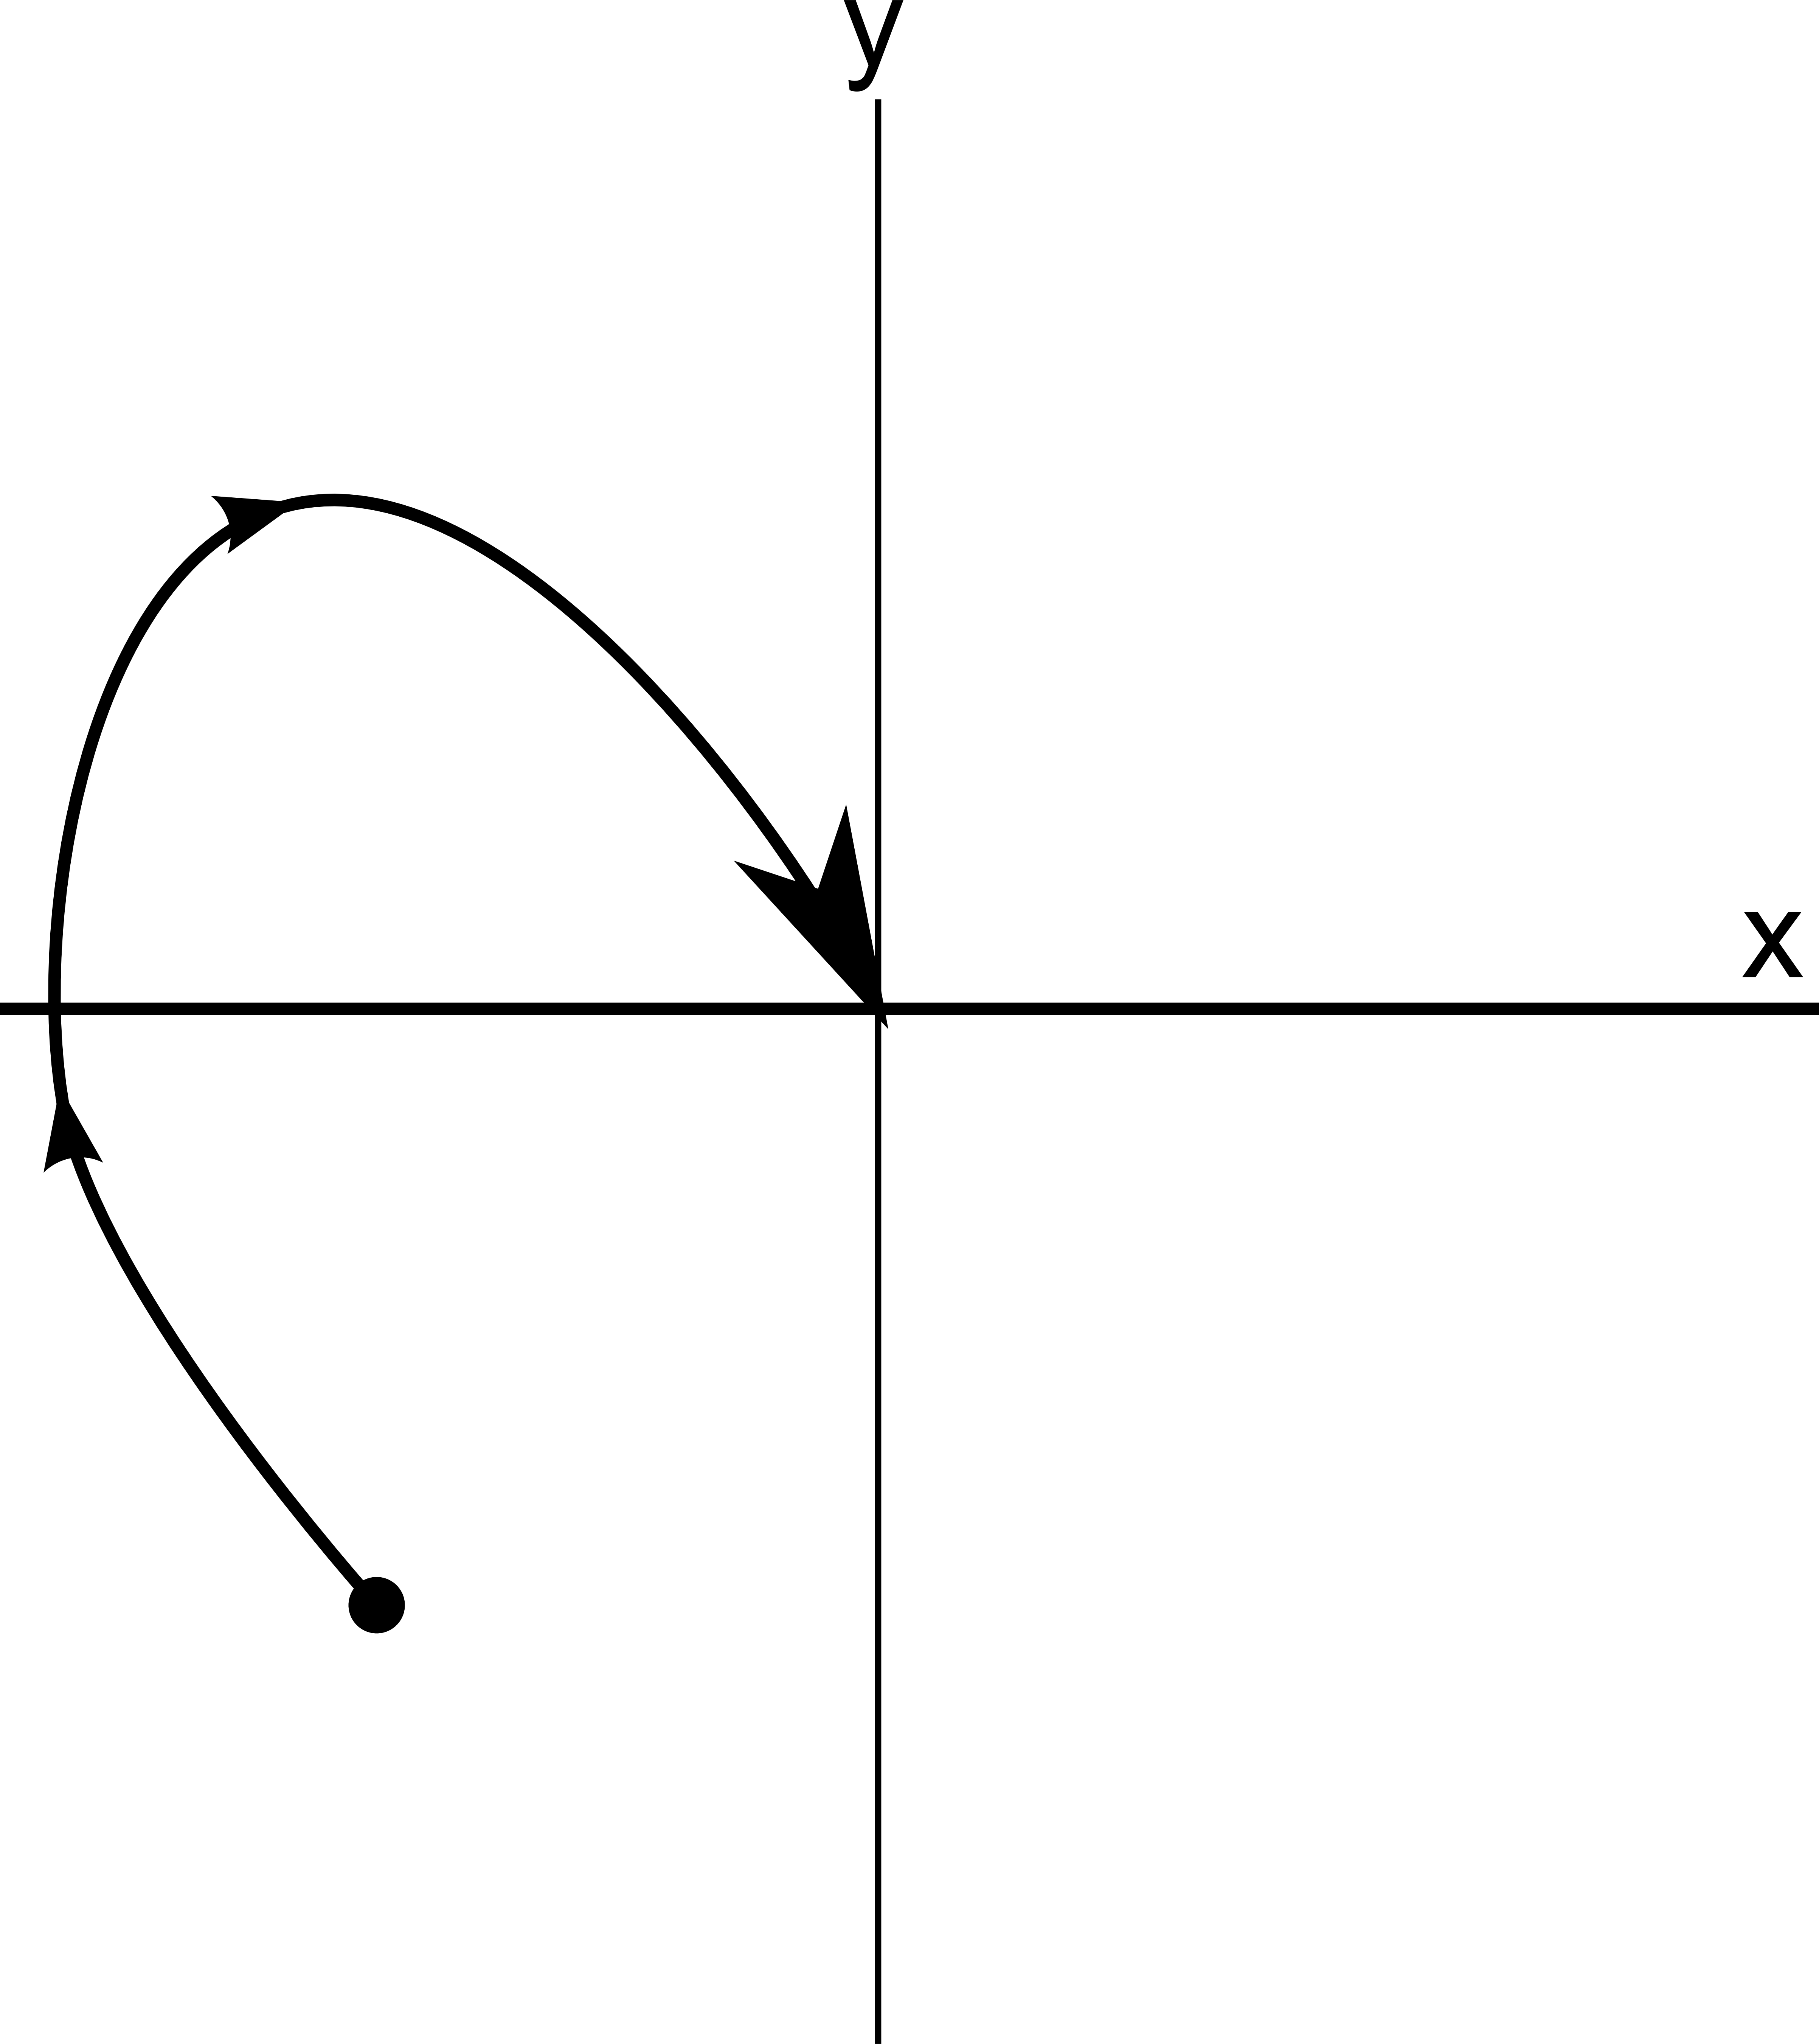
\includegraphics[width=4cm]{img/oneSystemSolution}}
  }

  \only<2->{%
    Phase plane: \\
    \centerline{\includegraphics[width=4cm]{img/phasePlane}}
  }
  

\end{frame}

\subsection{General Framework}

\begin{frame}
  \frametitle{General Solutions}

  \begin{eqnarray*}
    \deriv{~}{t} \vec{x}  & = & A \vec{x} + \vec{f}(t), \\
    \vec{x} & = & \vec{x}_h + \vec{x}_p, \\
    \vec{x}_h & = & \underbrace{C_1 \vec{x}_1(t) + C_2 \vec{x}_2(t) + \cdots + C_n \vec{x}_n(t)}_{n~\mathrm{linearly~independent~vectors}}, \\
    \vec{x}_h & = & \left[ \vec{x_1} \bigg| \vec{x_2} \bigg| \cdots \bigg| \vec{x_n} \right]
    \left[
      \begin{array}{rr}
        C_1 \\ C_2 \\ \vdots \\ C_n
      \end{array}
    \right].
  \end{eqnarray*}

  The vectors, $\vec{x}_i$, are related to the eigenvalues and the eigenvectors.

\end{frame}
\iftoggle{clicker}{%
\begin{frame}
  \frametitle{Clicker Quiz}

   \ifnum\value{clickerQuiz}=1{%
    \vfill

   \begin{eqnarray*}
     \deriv{~}{t} x & = &  4y, \\
     \deriv{~}{t} y & = & -2 x -3y.
   \end{eqnarray*}

   Written in matrix/vector form we get\\[12pt]

   \begin{tabular}{ll}
     A: & $\deriv{~}{t} \vecTwo{x}{y} =  
     \arrayTwo{0}{-2}{4}{-3} \vecTwo{x}{y}.$\\[12pt]
     B: & $\deriv{~}{t} \vecTwo{x}{y} =  
     \arrayTwo{0}{4}{-2}{-3} \vecTwo{x}{y}.$\\[12pt]
   \end{tabular}

   \vfill

 }\fi
  
 \ifnum\value{clickerQuiz}=2{%
   \vfill
   \begin{eqnarray*}
     \deriv{~}{t} x & = &  4y, \\
     \deriv{~}{t} y & = & -2 x -3y.
   \end{eqnarray*}

   Written in matrix/vector form we get\\[12pt]

   \begin{tabular}{ll}
     A: & $\deriv{~}{t} \vecTwo{x}{y} =  
     \arrayTwo{0}{4}{-2}{-3} \vecTwo{x}{y}.$\\[12pt]
     B: & $\deriv{~}{t} \vecTwo{x}{y} =  
     \arrayTwo{0}{-2}{4}{-3} \vecTwo{x}{y}.$\\[12pt]
   \end{tabular}

   \vfill

 }\fi
  
 \ifnum\value{clickerQuiz}=3{%
 \begin{eqnarray*}
    \deriv{~}{t} x & = &  y, \\
    \deriv{~}{t} y & = & -2 x -3y.
  \end{eqnarray*}

   Written in matrix/vector form we get\\[12pt]

   \begin{tabular}{ll}
     A: & $\deriv{~}{t} \vecTwo{x}{y} =  
      \arrayTwo{0}{1}{-2}{-3} \vecTwo{x}{y}.$\\[12pt]
     B: &  $\deriv{~}{t} \vecTwo{x}{y} =  
      \arrayTwo{1}{1}{-2}{-3} \vecTwo{x}{y}.$  \\
    \end{tabular}


        \vfill
 }\fi
\end{frame}
}


\begin{frame}
  \frametitle{Example}
  
  \begin{eqnarray*}
    \deriv{~}{t} x & = &  y, \\
    \deriv{~}{t} y & = & -2 x -3y.
  \end{eqnarray*}

  \uncover<2->
  {
    Written in matrix/vector form we get
    \begin{eqnarray*}
      \deriv{~}{t} \vecTwo{x}{y} & = & 
      \arrayTwo{0}{1}{-2}{-3} \vecTwo{x}{y}.
    \end{eqnarray*}
  }
  
\end{frame}

\begin{frame}
  \frametitle{Find the Eigenvalues and Eigenvectors}

  \begin{eqnarray*}
    A & = & \arrayTwo{0}{1}{-2}{-3}.
  \end{eqnarray*}

  \uncover<2->
  {
    \begin{eqnarray*}
      \begin{array}{rcl@{\hspace{2em}}rcl}
          \lambda_1 & = & -1, & \vec{v}_1 & = & \vecTwo{1}{-1}, \\
          \lambda_2 & = & -2, & \vec{v}_2 & = & \vecTwo{1}{-2}.
        \end{array}
    \end{eqnarray*}
  }

  \uncover<3->
  {
    The solution is
    \begin{eqnarray*}
       \vecTwo{x}{y} & = & C_1 e^{-t} \vecTwo{1}{-1}  + C_2 e^{-2t} \vecTwo{1}{-2}, \\
      x & = & C_1 e^{-t} + C_2 e^{-2t}, \\
      y & = & -C_1 e^{-t} - 2 C_2 e^{-2t}.
    \end{eqnarray*}
  }

\end{frame}


%\subsection{Reducing High Order Systems Using Systems}
\subsection{Reducing High Order Systems}

\begin{frame}
  \frametitle{Tricks of the Trade}

  Suppose that we have
  \begin{eqnarray*}
    x'' + 3x' + 2x & = & 0. \\
    \uncover<2->
    {
      \Rightarrow r^2 + 3r + 2 & = & 0, \\
      (r+2)(r+1) & = & 0, \\
      x & = & C_1 e^{-2t} + C_2 e^{-t}.
    }
  \end{eqnarray*}

\end{frame}


\begin{frame}
  \frametitle{Another Way to Look at It}

  We have
  \begin{eqnarray*}
    x'' + 3x' + 2x & = & 0.
  \end{eqnarray*}

  Let
  \begin{eqnarray*}
    x' & = & y, \\
    \uncover<2->
    {
      x'' & = & y', \\
      y' + 3y + 2x& = & 0, \\
      y' & = & -2x - 3y.
    }
  \end{eqnarray*}

  \uncover<3->
  {
    Written in matrix/vector form we get
    \begin{eqnarray*}
      \deriv{~}{t} \vecTwo{x}{y} & = & \arrayTwo{0}{1}{-2}{-3} \vecTwo{x}{y}.
    \end{eqnarray*}
  }

  \uncover<4->
  {
    \begin{eqnarray*}
      x(t)  & = & C_1 e^{-t} + C_2 e^{-2t}.
    \end{eqnarray*}
  }

\end{frame}


% LocalWords:  Clarkson pausesection hideothersubsections Vicini

\part{Solutions-to-Systems-of-DEs}
\lecture{Solutions to Systems of DEs}{Solutions-to-Systems-of-DEs}
\section{Solutions to Systems of DEs}


\title{Ordinary Differential Equations}
\subtitle{Math 232 - Solutions to Systems of Differential Equations}
\date{2 November 2012}

\begin{frame}
  \titlepage
\end{frame}

\begin{frame}
  \frametitle{Outline}
  \tableofcontents[pausesection,hideothersubsections]
\end{frame}


\subsection{Solutions to Systems of DEs}


\begin{frame}
  \frametitle{What is a solution to a System of DEs?}

  \begin{eqnarray*}
    \deriv{~}{t} \vec{x} & = & A \vec{x}.
  \end{eqnarray*}

  \uncover<2->
  {
    ``Looks'' like a first order, linear equation. The exponential has
    served us well in the past. Let's give it a try? Assume that 
    \begin{eqnarray*}
      \vec{x} & = & c e^{\lambda t} \vec{v}.
    \end{eqnarray*}
  }


\end{frame}


\begin{frame}
  \frametitle{Substitute it into the equation}

  The left hand Side:
  \begin{eqnarray*}
    \deriv{~}{t} \vec{x} & = & c \lambda e^{\lambda t} \vec{v} \\
  \end{eqnarray*}

  \uncover<2->
  {
    The right hand Side:
    \begin{eqnarray*}
      A \vec{x} & = & c e^{\lambda t} A \vec{v}.
    \end{eqnarray*}
  }

  \uncover<3->
  {
    Set them equal:
    \begin{eqnarray*}
      \Rightarrow c  e^{\lambda t} A \vec{v} & = & c \lambda e^{\lambda t} \vec{v}, \\
      A \vec{v} & = & \lambda \vec{v}.
    \end{eqnarray*}
  }

  \uncover<4->
  {
    This is an eigenvalue/eigenvector problem!
  }

\end{frame}


\begin{frame}
  \frametitle{Homogeneous Equations}

  Given
  \begin{eqnarray*}
    \deriv{~}{t} \vec{x} & = & A \vec{x},
  \end{eqnarray*}
  where $A$ is an $n\times n$ matrix, find the eigenvalues and
  eigenvectors. \textbf{If} there are \redText{$n$ linearly independent}
  eigenvectors then
  \begin{eqnarray*}
    \vec{x} & = & c_1 e^{\lambda_1 t} \vec{v}_1 + c_2 e^{\lambda_2 t} \vec{v}_2 +
    \cdot + c_n e^{\lambda_n t} \vec{v}_n.
  \end{eqnarray*}

\end{frame}

\subsection{Examples}

\iftoggle{clicker}{%
\begin{frame}
  \frametitle{Clicker Quiz}

   \ifnum\value{clickerQuiz}=1{%
\vfill


 }\fi

 \ifnum\value{clickerQuiz}=2{%
\vfill


 }\fi

 \ifnum\value{clickerQuiz}=3{%
  Given matrix 
  \begin{eqnarray*}
    A & = & \arrayTwo{5}{24}{-2}{-9}.
  \end{eqnarray*}
  Find the eigenvalues of $A$. 
  \begin{tabular}{ll}
          A: & $\lambda_1  = 5, \lambda_2 = -9$ \\
          B: & $\lambda_1  = -1, \lambda_2 = -3$ \\
          C: & $\lambda_1  = 2, \lambda_2 = -2$ \\
        \end{tabular}

  \vfill
 }\fi
\end{frame}
}


\begin{frame}
  \frametitle{Example}

  \begin{eqnarray*}
    \deriv{~}{t} \vec{x} & = & \arrayTwo{5}{24}{-2}{-9} \vec{x}.
  \end{eqnarray*}

  \uncover<2->
  {
    First find the eigenvalues,
    \begin{eqnarray*}
      0 & = & \det\lp\arrayTwo{5-\lambda}{24}{-2}{-9-\lambda}\rp, \\
      & = & (\lambda+1)(\lambda+3).
    \end{eqnarray*}
    The eigenvalues are \redText{$\lambda_1=-1$} and \blueText{$\lambda_2=-3$}.
  }

\end{frame}


\begin{frame}
  \frametitle{Find the eigenvectors}

  $\lambda_1 = -1$:
  \begin{eqnarray*}
    \arrayTwo{6}{24}{-2}{-8} \vecTwo{x}{y} & = & \vecTwo{0}{0}, \\
    6x + 24y & = & 0, \\
    -2x - 8y & = & 0, \\
    \uncover<2->
    {
      \Rightarrow \redText{\vec{v}_1} & \redText{=} & \redText{\vecTwo{-4}{1}}.
    }
  \end{eqnarray*}

  \uncover<3->
  {
    $\lambda_2 = -3$:
    \begin{eqnarray*}
      \arrayTwo{8}{24}{-2}{-6} \vecTwo{x}{y} & = & \vecTwo{0}{0}, \\
      8x + 24y & = & 0, \\
      -2x - 6y & = & 0, \\
      \uncover<4->
      {
        \Rightarrow \blueText{\vec{v}_2} & \blueText{=} & \blueText{\vecTwo{-3}{1}}.
      }
    \end{eqnarray*}
  }

\end{frame}


\begin{frame}
  \frametitle{Assemble the Solution}

  \begin{eqnarray*}
    \vec{x}(t) & = & \redText{c_1 e^{-t} \vecTwo{-4}{1}} + \blueText{c_2 e^{-3t} \vecTwo{-3}{1}}.
  \end{eqnarray*}

\end{frame}

\begin{frame}
  \frametitle{Example}

  \begin{eqnarray*}
    x'' + 5x' + 6x & = & 0, \\
    \Rightarrow x_h & = & C_1 e^{-3t} + C_2 e^{-2t}.
  \end{eqnarray*}

  \uncover<2->
  {
    Let $x'=y$,
    \begin{eqnarray*}
      x' & = & y, \\
      y' & = & -6x - 5y,
    \end{eqnarray*}
    which leads to the following system
    \begin{eqnarray*}
      \deriv{~}{t} \vec{x} & = & \arrayTwo{0}{1}{-6}{-5} \vec{x}.
    \end{eqnarray*}
  }

\end{frame}

\begin{frame}
    \frametitle{First find the eigenvalues}
    \begin{eqnarray*}
      0 & = & \det\lp\arrayTwo{-\lambda}{1}{-6}{-5-\lambda}\rp, \\
      & = & (\lambda+2)(\lambda+3).
    \end{eqnarray*}
    The eigenvalues are $\lambda_1=-2$ and $\lambda_2=-3$.

\end{frame}

\iftoggle{clicker}{%
\begin{frame}
  \frametitle{Clicker Quiz}

   \ifnum\value{clickerQuiz}=1{%
     \vfill
   }\fi

   \ifnum\value{clickerQuiz}=2{%
   \vfill
   }\fi

  \ifnum\value{clickerQuiz}=3{%
   For  $\lambda_1 = -2$, find the corresponding eigenvectors.
   \begin{tabular}{ll}
          A: & $\vec{v}_1  =  \vecTwo{1}{-2}.$ \\
          B: & $\vec{v}_1  =  \vecTwo{2}{1}.$ \\
          C: & $\vec{v}_1  =  \vecTwo{1}{2}.$ \\
        \end{tabular}

  \vfill
 }\fi
\end{frame}
}


\begin{frame}
  \frametitle{Find the eigenvectors}

  $\lambda_1 = -2$:
  \begin{eqnarray*}
    \arrayTwo{2}{1}{-6}{-3} \vecTwo{x}{y} & = & \vecTwo{0}{0}, \\
    2x + y & = & 0, \\
    -6x - 3y & = & 0, \\
    \uncover<2->
    {
      \Rightarrow \redText{\vec{v}_1} & \redText{=} & \redText{\vecTwo{1}{-2}}.
    }
  \end{eqnarray*}

  \uncover<3->
  {
    $\lambda_2 = -3$:
    \begin{eqnarray*}
      \arrayTwo{3}{1}{-6}{-2} \vecTwo{x}{y} & = & \vecTwo{0}{0}, \\
      3x + y & = & 0, \\
      -6x - 2y & = & 0, \\
      \uncover<4->
      {
        \Rightarrow \blueText{\vec{v}_2} & \blueText{=} & \blueText{\vecTwo{1}{-3}}.
      }
    \end{eqnarray*}
  }

\end{frame}


\begin{frame}
  \frametitle{Assemble the Solution}

  \begin{eqnarray*}
    \vec{x}(t) & = & \redText{c_1 e^{-2t} \vecTwo{1}{-2}} + \blueText{c_2 e^{-3t} \vecTwo{1}{-3}}.
  \end{eqnarray*}

  \uncover<2->
  {
    The Phase Plane:\\
    \centerline{\includegraphics[width=4cm]{img/phasePlaneExample}}

  }
  

\end{frame}


\begin{frame}
  \frametitle{Solution Behaviors and Nomenclature}

  \begin{columns}
    \column{.33\textwidth} \includegraphics[width=3cm]{img/phasePlaneSink}
    \column{.33\textwidth} \includegraphics[width=3cm]{img/phasePlaneSource}
    \column{.33\textwidth} \includegraphics[width=3cm]{img/phasePlaneSaddle}
  \end{columns}  

\end{frame}


\subsection{Repeated Eigenvalues}
\begin{frame}
  \frametitle{Example}
  \begin{eqnarray*}
    \deriv{~}{t} \vec{x} & = & \arrayTwo{2}{0}{0}{2} \vec{x}.
  \end{eqnarray*}
  \uncover<2->
  {
    Find the eigenvalues,
    \begin{eqnarray*}
      0 & = & \det\lp\arrayTwo{2-\lambda}{0}{0}{2-\lambda}\rp, \\
      & = & (2-\lambda)^2.
    \end{eqnarray*}
    The eigenvalue is $\lambda=2$.
  }
\end{frame}

\begin{frame}
  \frametitle{Find the Eigenvector}
  $\lambda_1=2$:
  \begin{eqnarray*}
    \arrayTwo{0}{0}{0}{0} \vecTwo{x}{y} & = & \vecTwo{0}{0}, \\
    \uncover<2->
    {
      \Rightarrow \vec{v} & = & \vecTwo{x}{y}, \\
      & = & x \vecTwo{1}{0} + y \vecTwo{0}{1}, \\
      \uncover<3->
      {
        \vec{v}_1 & = & \vecTwo{1}{0}, \\
        \vec{v}_2 & = & \vecTwo{0}{1}.
      }
    }
  \end{eqnarray*}
\end{frame}

\begin{frame}
  \frametitle{Form the Solution}
  The solution is
  \begin{eqnarray*}
    \vec{x} & = & c_1 e^{2t} \vecTwo{1}{0} + c_2 e^{2t} \vecTwo{0}{1}.
  \end{eqnarray*}
\end{frame}


\begin{frame}
  \frametitle{Example}

  \begin{eqnarray*}
    \deriv{~}{t} \vec{x} & = & \arrayTwo{0}{-1}{4}{-4} \vec{x}.
  \end{eqnarray*}

  \uncover<2->
  {
    Find the eigenvalues:
    \begin{eqnarray*}
      0 & = & \det\lp\arrayTwo{-\lambda}{-1}{4}{-4-\lambda}\rp, \\
      & = & \lp \lambda + 2 \rp^2,
    \end{eqnarray*}
    The value of $\lambda$ is -2.
  }

\end{frame}


\begin{frame}
  \frametitle{Find the eigenvectors}

  \begin{eqnarray*}
    \arrayTwo{2}{-1}{4}{-2} \vec{x}{y} & = & \vecTwo{0}{0}, \\
    2x - y & = & 0, \\
    4x - 2y & = & 0.
  \end{eqnarray*}

  There is only one eigenvector,
  \begin{eqnarray*}
    \vec{v}_1 & = & \vecTwo{1}{2}.
  \end{eqnarray*}
  One homogeneous solution is 
  \begin{eqnarray*}
   \vec{x}_1 & = & e^{-2t}\vecTwo{1}{2}.
  \end{eqnarray*}

\end{frame}

\begin{frame}
  \frametitle{What to do?}

  Last time this happened we tried to multiply by $t$, and it
  worked. We will try that again...
  Assume that
  \begin{eqnarray*}
    \vec{x} & = & t e^{\lambda t} \vec{v} + e^{\lambda t} \vec{u}.
  \end{eqnarray*}

  \uncover<2->
  {
    Substitute back into the equation:
    \begin{eqnarray*}
      \deriv{~}{t} \vec{x} & = & \lambda t e^{\lambda t} \vec{v} + e^{\lambda t} \vec{v} 
         + \lambda e^{\lambda t} \vec{u}, \\
      A\vec{x} & = & t e^{\lambda t} A \vec{v} + e^{\lambda t} A \vec{u}.
    \end{eqnarray*}
  }
  
\end{frame}


\begin{frame}
  \frametitle{Set The Two Expressions Equal}

  \only<1>
  {
    \begin{eqnarray*}
      \lambda t e^{\lambda t} \vec{v} + e^{\lambda t} \vec{v} + \lambda e^{\lambda t} \vec{u}
      & = & 
      t e^{\lambda t} A \vec{v} + e^{\lambda t} A \vec{u}.
    \end{eqnarray*}
  }

  \only<2->
  {
    \begin{eqnarray*}
      \redText{\underbrace{\lambda t e^{\lambda t} \vec{v}}_ {te^{\lambda t}}} +  
      \blueText{\underbrace{e^{\lambda t} \vec{v} + \lambda e^{\lambda t} \vec{u}}_{e^{\lambda t}}}
      & = & 
      \redText{\underbrace{t e^{\lambda t} A \vec{v}}_{t e^{\lambda t}}} + 
      \blueText{\underbrace{e^{\lambda t} A \vec{u}}_{e^{\lambda t}}}.
    \end{eqnarray*}

    Match the like terms.

  }
  

\end{frame}

\begin{frame}
  \frametitle{Set The Two Expressions Equal}

    \begin{eqnarray*}
      \redText{\lambda t e^{\lambda t} \vec{v}} + \blueText{e^{\lambda t} \vec{v} + \lambda e^{\lambda t} \vec{u}}
      & = & 
      \redText{t e^{\lambda t} A \vec{v}} + \blueText{e^{\lambda t} A \vec{u}}.
    \end{eqnarray*}
  
    This has to be true for all $t$ so we have the following equations:
    \begin{eqnarray*}
      \redText{\lambda t e^{\lambda t} \vec{v}} & \redText{=} & \redText{t e^{\lambda t} A \vec{v}}, \\
      \lambda \vec{v} & = & A \vec{v}.
    \end{eqnarray*}
    (This is the eigenvalue and eigenvector!)

    We also have 
    \begin{eqnarray*}
      \blueText{e^{\lambda t} \vec{v} + \lambda e^{\lambda t} \vec{u}} & \blueText{=} & \blueText{e^{\lambda t} A \vec{u}} , \\
      \vec{v} + \lambda \vec{u} & = &  A \vec{u}, \\
      \Rightarrow \lp A - \lambda I \rp \vec{u} & = & \vec{v}.
    \end{eqnarray*}

\end{frame}


\begin{frame}
  \frametitle{Back to the Example}

  \begin{eqnarray*}
    \deriv{~}{t} \vec{x} & = & \arrayTwo{0}{-1}{4}{-4} \vec{x}.
  \end{eqnarray*}


  There is only one eigenvalue, $\lambda=-2$ with one eigenvector,
  \begin{eqnarray*}
    \vec{v}_1 & = & \vecTwo{1}{2}.
  \end{eqnarray*}
  One homogeneous solution is 
  \begin{eqnarray*}
   \vec{x}_1 & = & e^{-2t}\vecTwo{1}{2}.
  \end{eqnarray*}


\end{frame}


\begin{frame}
  \frametitle{Finding the other solution}

  Assume a solution in the form
  \begin{eqnarray*}
    \vec{x} & = & t e^{-2 t} \vecTwo{1}{2} + e^{-2 t} \vec{u}, \\
    \arrayTwo{2}{-1}{4}{-2} \vecTwo{x}{y} & = & \vecTwo{1}{2}, \\
    2x-y & = & 1 \\
    4x-2y & = & 2.
  \end{eqnarray*}

  The vector, $\vec{u}$, is the following:
  \begin{eqnarray*}
    \vec{u} & = & \vecTwo{0}{-1}+\vecTwo{1}{2}x. 
  ~~~~\text{Let }  \vec{u}  =  \vecTwo{0}{-1}.
  \end{eqnarray*}
  One homogeneous solution is:
  \begin{eqnarray*}
    \vec{x}_2 & = & te^{-2t}\vecTwo{1}{2}+e^{-2t}\vecTwo{0}{-1} 
     =  e^{-2t}\vecTwo{t}{2t-1}.
  \end{eqnarray*}

\end{frame}

\begin{frame}
  \frametitle{Form the Solution}
  
  The solution to the differential equation is
  \begin{eqnarray*}
    \vec{x}(t) & = &  C_1 e^{-2t} \vecTwo{1}{2} + C_2 e^{-2t}\vecTwo{t}{2t-1}.
  \end{eqnarray*}
\end{frame}


\subsection{Coupled Tank Problems}


\begin{frame}
  \frametitle{Coupled Tank}

  \only<1>{\centerline{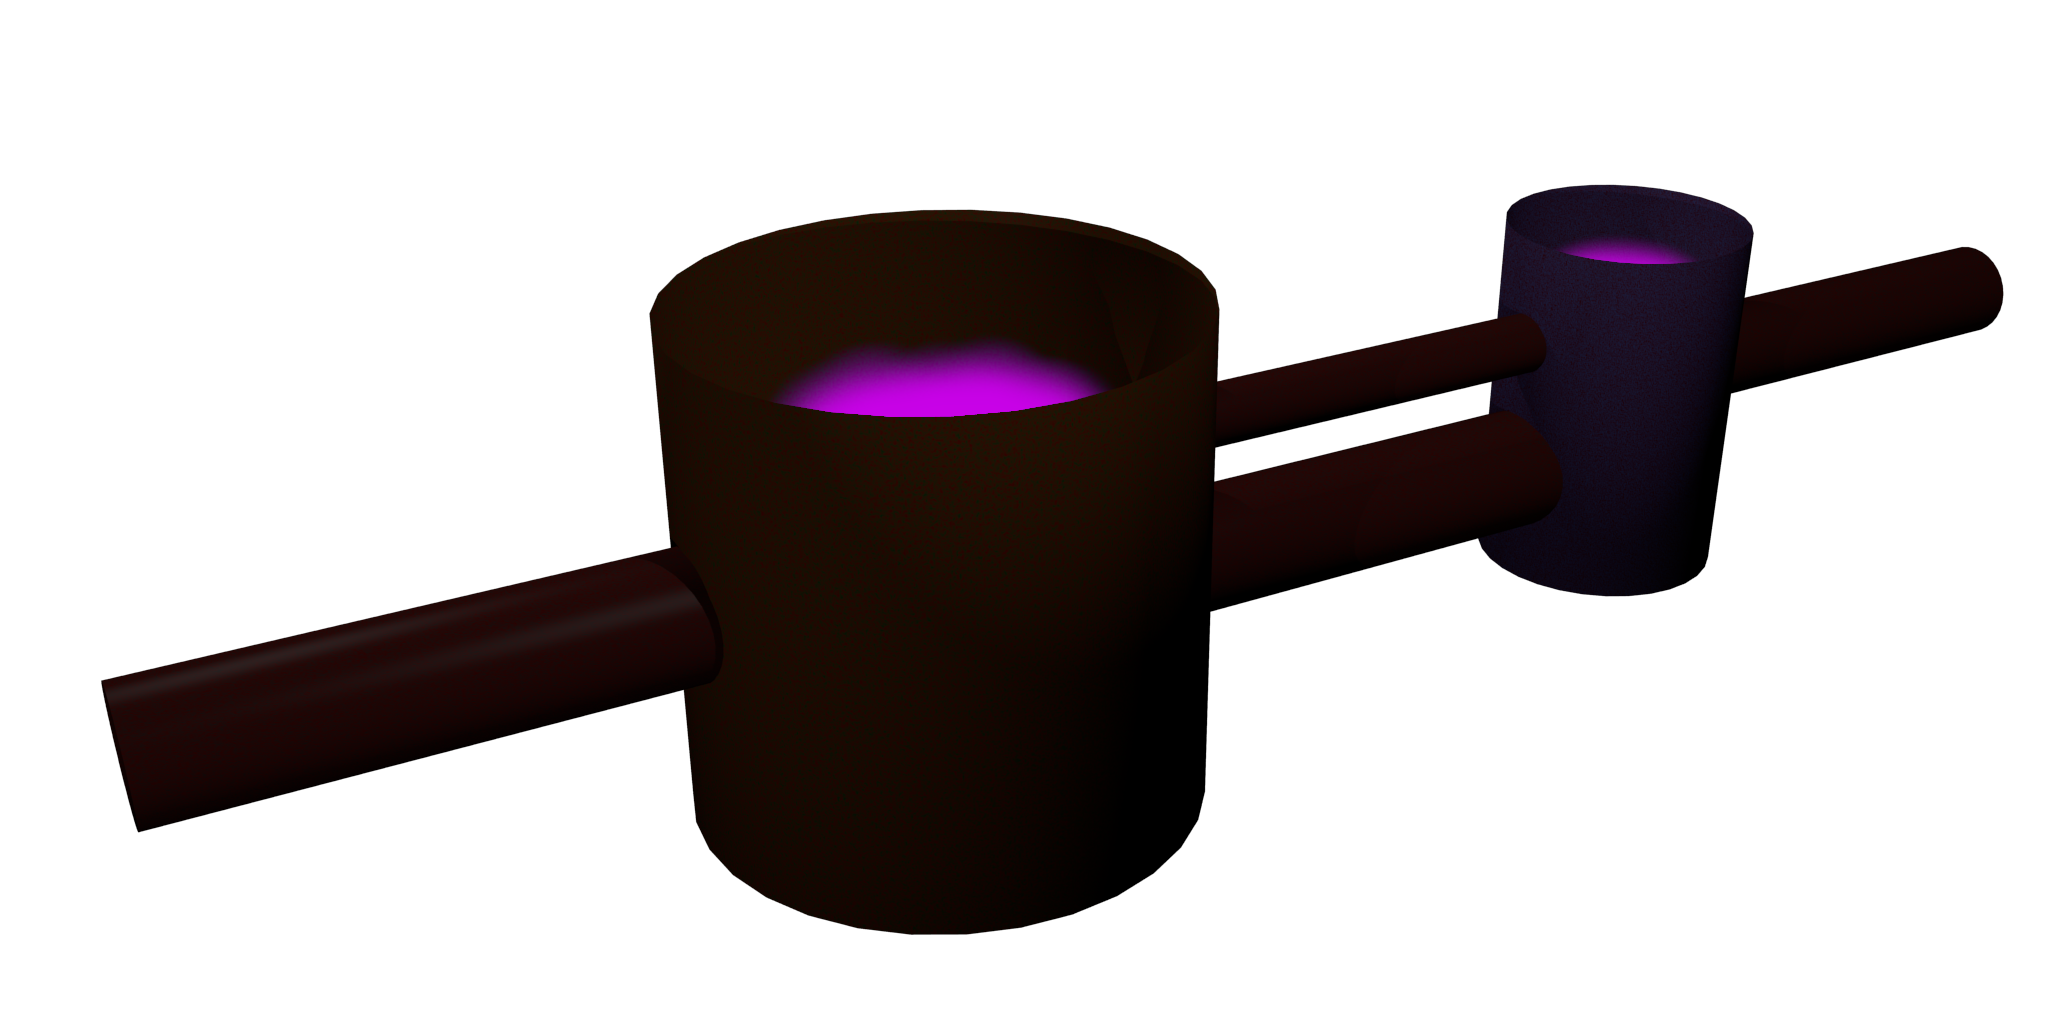
\includegraphics[width=9cm]{img/doubleTank}}}
  \only<2>{\centerline{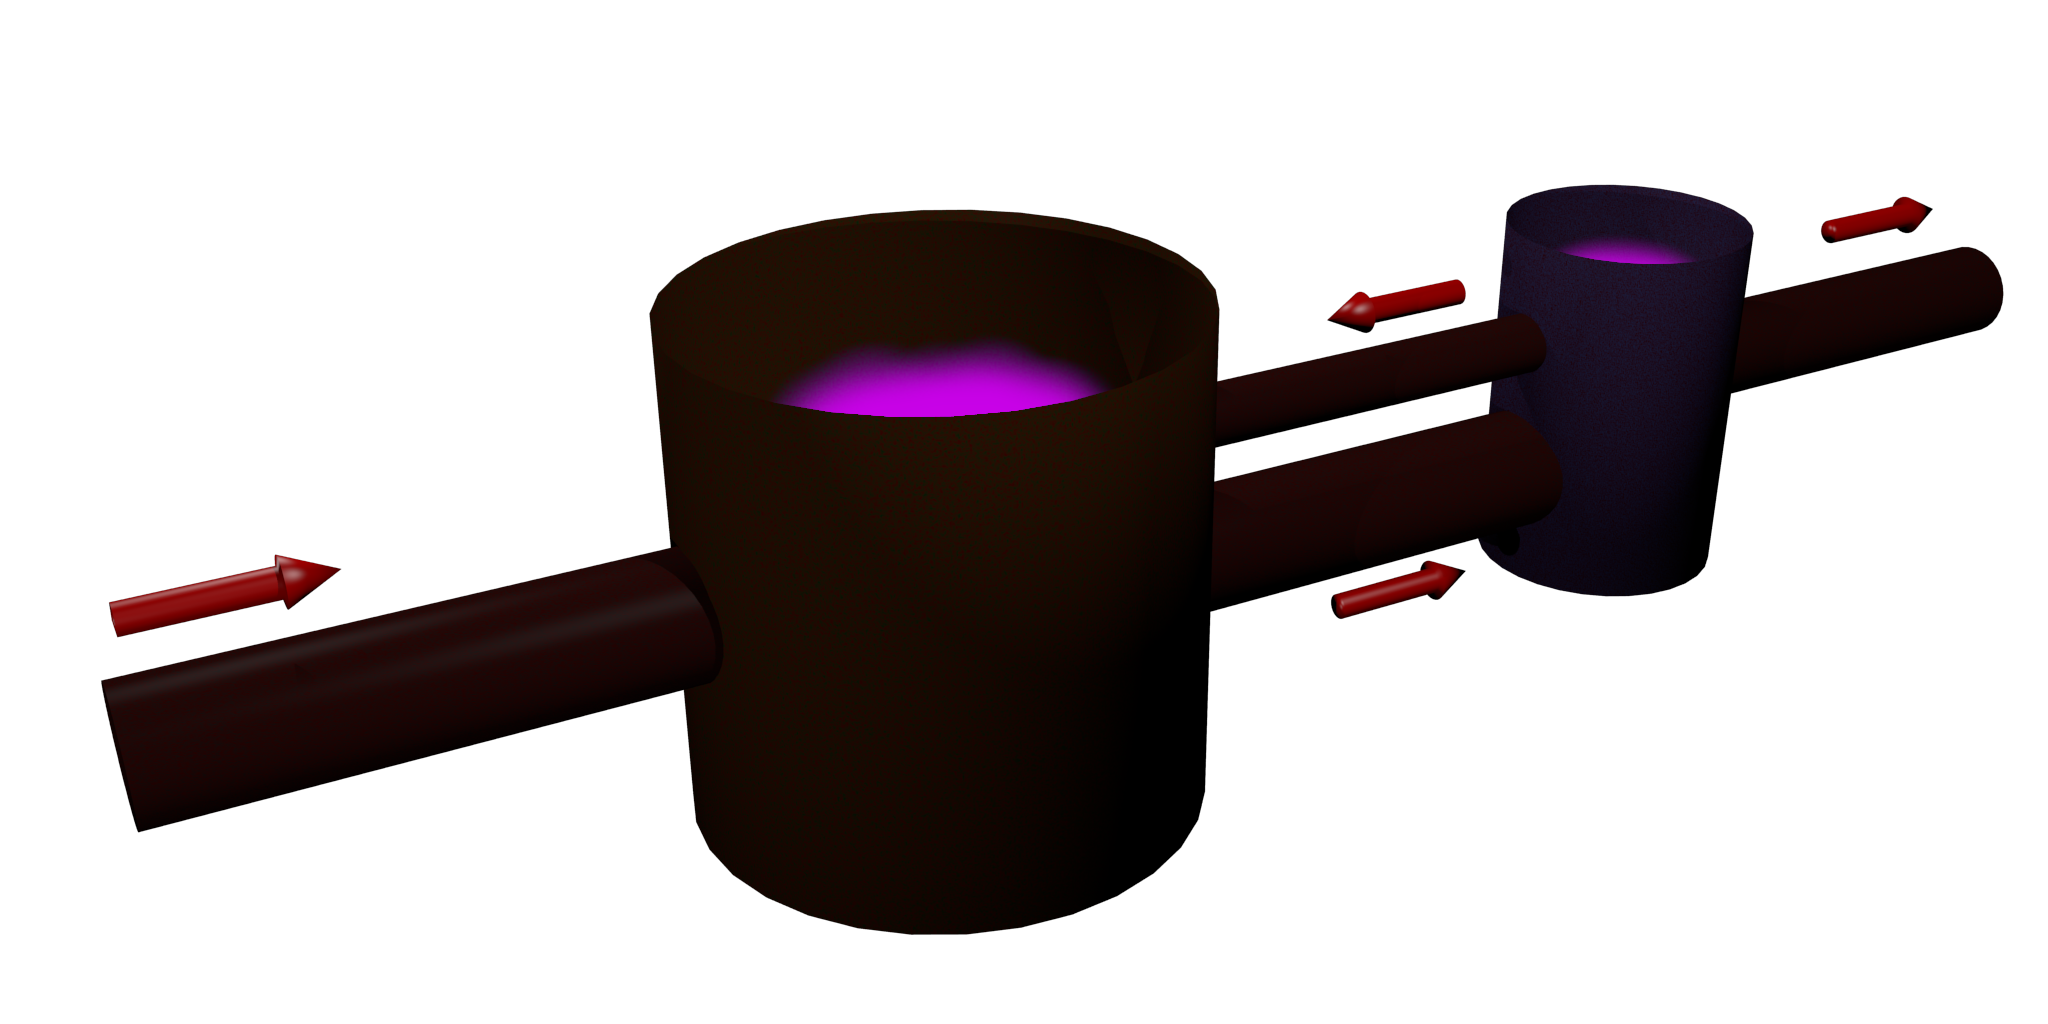
\includegraphics[width=9cm]{img/doubleTankArrows}}}
  \only<3>{\centerline{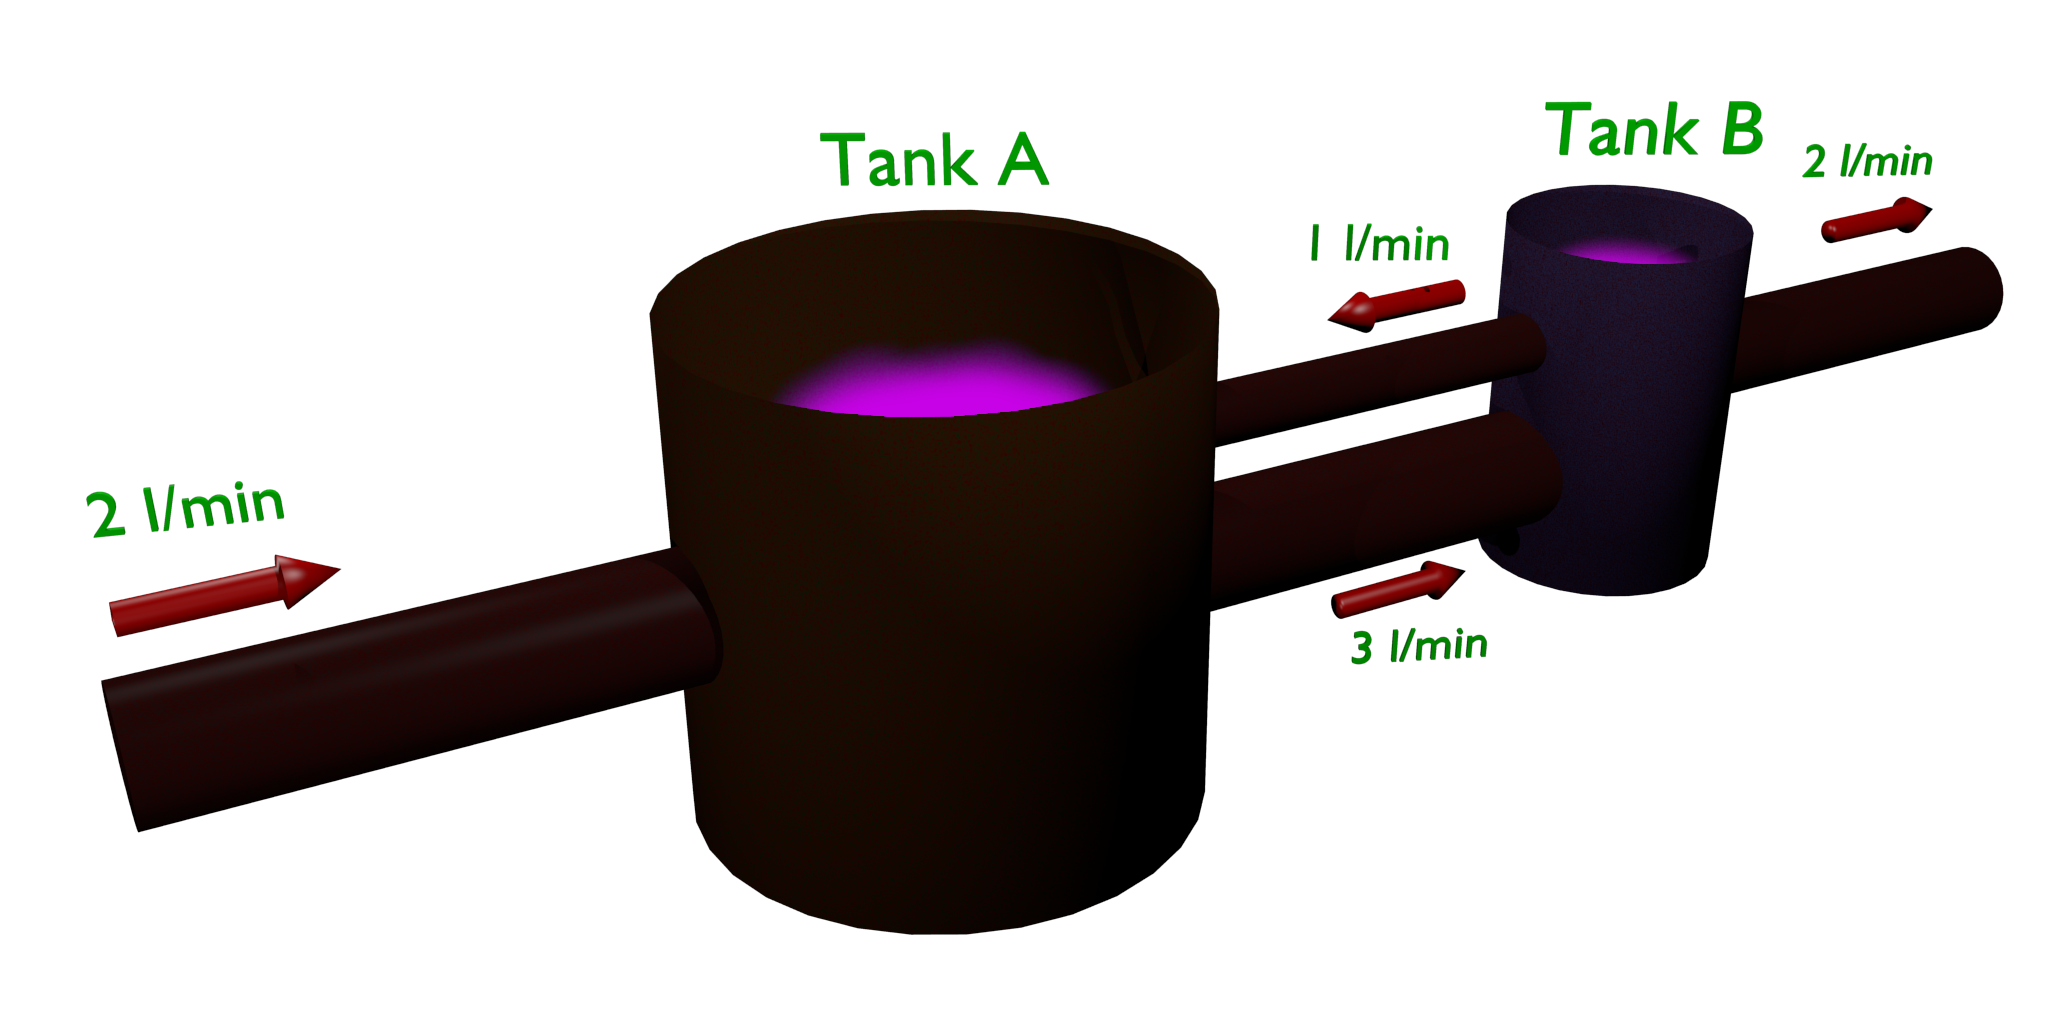
\includegraphics[width=9cm]{img/doubleTankAnnotated}}}

  Two tanks are arranged as shown. Initially tank A has 100 liters of
  water and tank B has 50 liters of water. Initially each tank has 2
  kg of salt dissolved in the solution. Pure water is pumped into to
  the first tank at a rate of 2 liters per minute. The solution in the
  second tank is pumped out a rate of 2 liters per minute. Determine
  the amount of salt in each tank at any time.
  
\end{frame}


\begin{frame}
  \frametitle{System of Equations}

  $x(t)$ is the amount of salt in tank A at time $t$.

  $y(t)$ is the amount of salt in tank B at time $t$.

  \begin{eqnarray*}
    \deriv{x}{t} & = & 0\times 2 - 
    \frac{x}{100}\times 3 + \frac{y}{50}\times 2 \\
    \deriv{y}{t} & = & \frac{x}{100} \times 3 -
    \frac{y}{50} \times 1 - \frac{y}{50}\times 2.
  \end{eqnarray*}

  Written as a system we get
  \begin{eqnarray*}
    \deriv{~}{t} \vecTwo{x}{y} & = & 
    \arrayTwo{-3/100}{2/50}{3/100}{-3/50} \vecTwo{x}{y}.
  \end{eqnarray*}
  
\end{frame}


% LocalWords:  Clarkson pausesection hideothersubsections eigenvector
% LocalWords:  eigenvectors

\part{Complex-Eigen-Values}
\lecture{Complex Eigenvalues}{Complex-Eigen-Values}
\section{Complex Eigenvalues}


\title{Ordinary Differential Equations}
\subtitle{Math 232 - Week 11, Day 1}
\date{5 November 2012}

\begin{frame}
  \titlepage
\end{frame}

\begin{frame}
  \frametitle{Outline}
  \tableofcontents[pausesection,hideothersubsections]
\end{frame}


\subsection{Complex Valued Eigenvalues}


\begin{frame}
  \frametitle{Complex Valued Eigenvalues}

  First, recall:
  \begin{eqnarray*}
    e^{a+bi} & = & e^a e^{bi}, \\
    & = & e^a \lp \cos(b) + i \sin(b) \rp.
  \end{eqnarray*}

  Also, the complex conjugate:
  \begin{eqnarray*}
    \overline{a+ib} & = & a-i b.
  \end{eqnarray*}

  Note: If A is a real valued matrix with complex valued eigenvalues,
  then the eigenvalues and eigenvectors come in complex conjugates
  pairs.

\end{frame}

\iftoggle{clicker}{%
\begin{frame}
  \frametitle{Clicker Quiz}

   \ifnum\value{clickerQuiz}=1{%
     \vfill
   }\fi

   \ifnum\value{clickerQuiz}=2{%
   \vfill
   }\fi

  \ifnum\value{clickerQuiz}=3{%
   Given $A=\arrayTwo{5}{-10}{1}{-1}$. Find the eigenvalues.
   \begin{tabular}{ll}
          A: & $\lambda_{1,2} = 2 \pm i.$ \\
          B: & $\lambda_{1} = 5, \lambda_2 = -1.$ \\
          C: & $\lambda_{1,2} = 2.$ \\
        \end{tabular}

  \vfill
 }\fi
\end{frame}
}


\begin{frame}
  \frametitle{Example}

  \begin{eqnarray*}
    \deriv{~}{t} \vec{x} & = & \arrayTwo{5}{-10}{1}{-1} \vec{x}.
  \end{eqnarray*}

  \uncover<2->
  {
    Find the eigenvalues:
    \begin{eqnarray*}
      \det\lp\arrayTwo{5-\lambda}{-10}{1}{-1-\lambda}\rp 
      & = & \lambda^2-4\lambda+5 \\
      \lambda_{1,2} & = & 2 \pm i.
    \end{eqnarray*}
  }

\end{frame}


\begin{frame}
  \frametitle{Find the Eigenvectors}

  $\lambda_1 = 2+i$:
  \begin{eqnarray*}
    \arrayTwo{3-i}{-10}{1}{-3-i} \vecTwo{x}{y} & = & \vecTwo{0}{0} \\
    x & = & \lp 3 + i \rp y, \\
    \Rightarrow \vec{v}_1 & = & y \lp \vecTwo{3}{1} + \vecTwo{i}{0} \rp.
  \end{eqnarray*}

  \uncover<2->
  {
    $\lambda_2 = 2-i$:
    \begin{eqnarray*}
      \arrayTwo{3+i}{-10}{1}{-3+i} \vecTwo{x}{y} & = & \vecTwo{0}{0} \\
      x & = & \lp 3-i \rp y, \\
      \Rightarrow \vec{v}_2 & = & y \lp \vecTwo{3}{1} - \vecTwo{i}{0} \rp.
    \end{eqnarray*}
  }

\end{frame}


\begin{frame}
  \frametitle{Determine the Solution}

  \begin{eqnarray*}
    \uncover<1->
    {
      \vec{x} & = & A e^{(2+i)t} \lp \vecTwo{3}{1} + \vecTwo{i}{0} \rp
      + B e^{(2-i)t} \lp \vecTwo{3}{1} - \vecTwo{i}{0} \rp \\
    }
    \uncover<2->
    {
      \vec{x} & = & A e^{(2+i)t} \lp \underbrace{\vecTwo{3}{1}}_{\vec{p}} + 
      \underbrace{\vecTwo{i}{0}}_{i\vec{q}} \rp
      + B e^{(2-i)t} \lp \underbrace{\vecTwo{3}{1}}_{\vec{p}} -
      \underbrace{\vecTwo{i}{0}}_{i\vec{q}} \rp \\
    }
    \uncover<3->
    {
      & = & e^{2t} \lp
      A\lp \cos(t) + i \sin(t) \rp \lp \vec{p} + i \vec{q} \rp 
      + B \lp \cos(t) - i \sin(t) \rp \lp \vec{p} - i \vec{q} \rp 
      \rp
    }
  \end{eqnarray*}

\end{frame}


\begin{frame}
  \frametitle{More Algebra...}

  \begin{eqnarray*}
    \vec{x} & = & e^{2t} \lp
      A\lp \cos(t) + i \sin(t) \rp \lp \vec{p} + i \vec{q} \rp 
      + B \lp \cos(t) - i \sin(t) \rp \lp \vec{p} - i \vec{q} \rp 
      \rp \\
      & = & C_1 e^{2t} \lp \cos(t) \vec{p} - \sin(t) \vec{q} \rp
      + C_2 e^{2t} \lp \cos(t) \vec{q} + \sin(t) \vec{p} \rp.
  \end{eqnarray*}

  (The solutions spiral out.)

\end{frame}

\subsection{Characterization of Solutions}

\begin{frame}
  \frametitle{Characterization of Solutions}

  \begin{eqnarray*}
    \deriv{~}{t} \vec{x} & = & A \vec{x}.
  \end{eqnarray*}

  If $\lambda$'s are complex, $\lambda = a \pm ib$:
  \begin{enumerate}
  \item If $\alpha>0$ then it is a repelling spiral.
  \item If $\alpha<0$ then it is an attracting spiral.
  \item If $\alpha=0$ then the solutions are neutrally stable.
  \end{enumerate}

\end{frame}


\subsection{Nullclines}

\begin{frame}
  \frametitle{Nullclines}

  Given a solution to a differential equation,
  \begin{eqnarray*}
    \vec{x} & = & \vecTwo{x(t)}{y(t)},
  \end{eqnarray*}
  if
  \begin{itemize}
  \item $x'(t)=0$ then the trajectory is ``vertical'' at time $t$,
  \item $y'(t)=0$ then the trajectory is ``horizontal'' at time $t$.
  \end{itemize}

\end{frame}


\begin{frame}
  \frametitle{Definition of the Nullclines}

  The set of points, $\vecTwo{x}{y}$ where $x'(t)=0$ is called the v-nullcline. (Vertical slope.)

  The set of points, $\vecTwo{x}{y}$ where $y'(t)=0$ is called the h-nullcline. (Horizontal slope.)

\end{frame}


\begin{frame}
  \frametitle{Example}
  
  In the previous example we had
  \begin{eqnarray*}
    \deriv{~}{t} \vec{x} & = & \arrayTwo{5}{-10}{1}{-1} \vec{x}.
  \end{eqnarray*}

  \uncover<2->
  {
    Find the v-nullcline:
    \begin{eqnarray*}
      \deriv{x}{t} & = & 5x - 10y, \\
      0 & = & 5x - 10y, \\
      y & = & \frac{1}{2} x.
    \end{eqnarray*}
  }

  \uncover<3->
  {
    Find the h-nullcline:
    \begin{eqnarray*}
      \deriv{y}{t} & = & x - y, \\
      0 & = & x - y, \\
      y & = &  x.
    \end{eqnarray*}
  }


\end{frame}



% LocalWords:  Clarkson pausesection hideothersubsections

\part{Trace-Determinant-Plane}
\lecture{Trace-Determinant Plane}{Trace-Determinant-Plane}
\section{Trace-Determinant Plane}


\title{Ordinary Differential Equations}
\subtitle{Math 232 - The Trace Determinant Plane}
\date{7 November 2012}

\begin{frame}
  \titlepage
\end{frame}

\begin{frame}
  \frametitle{Outline}
  \tableofcontents[pausesection,hideothersubsections]
\end{frame}


\subsection{Behavior of Solutions to DEs}


\begin{frame}
  \frametitle{Behavior of Solutions to DEs}

  The eigenvalues determine the stability characteristics of the
  system of DEs.

  If the eigenvalues are \blueText{real}:
  \begin{itemize}
  \item $\lambda_2 < \lambda_1 < 0$ - Sink
  \item $\lambda_2 < 0 < \lambda_1$ - Saddle
  \item $0 < \lambda_2 < \lambda_1$ - Source
  \end{itemize}

  If the eigenvalues are \blueText{complex}, $\lambda_{1,2}=\redText{a}+ib$:
  \begin{itemize}
  \item $\redText{a}<0$ - Attracting spiral
  \item $\redText{a}>0$ - Repelling spiral
  \item $\redText{a}=0$ - Center
  \end{itemize}

\end{frame}

\iftoggle{clicker}{%
\begin{frame}
  \frametitle{Clicker Quiz}

   \ifnum\value{clickerQuiz}=1{%
   The matrix for a  system of equations,
   \begin{eqnarray*}
     \deriv{~}{t} \vec{x} & = & A \vec{x},
   \end{eqnarray*}
   has eigenvalues $\lambda_1=-2+\sqrt{3}i$ and
   $\lambda_1=-2-\sqrt{3}i$. What is the general behavior of the
   resulting system?

     \begin{tabular}{ll}
       A: &  Source \\
       B: &  Sink \\
       C: &  Spiral Source \\
       D: &  Spiral Sink
     \end{tabular}

     \vfill


 }\fi

 \ifnum\value{clickerQuiz}=2{%

   The matrix for a  system of equations,
   \begin{eqnarray*}
     \deriv{~}{t} \vec{x} & = & A \vec{x},
   \end{eqnarray*}
   has eigenvalues $\lambda_1=2+\sqrt{3}i$ and
   $\lambda_1=2-\sqrt{3}i$. What is the general behavior of the
   resulting system?

     \begin{tabular}{ll}
       A: &  Source \\
       B: &  Sink \\
       C: &  Spiral Source \\
       D: &  Spiral Sink
     \end{tabular}

     \vfill

 }\fi

 \ifnum\value{clickerQuiz}=3{%
  \vfill
 }\fi
\end{frame}
}


\subsection{Special Case of $2\times 2$ Systems}

\begin{frame}
  \frametitle{Special Case of $2\times 2$ Systems}

  \begin{eqnarray*}
    \deriv{~}{t} \vec{x} & = & \arrayTwo{a}{b}{c}{d} \vec{x}, \\
    & = & A \vec{x}.
  \end{eqnarray*}

  \uncover<2->
  {
    Find the eigenvalues:
    \begin{eqnarray*}
      \only<2>
      {
        \det\lp\arrayTwo{a-\lambda}{b}{c}{d-\lambda}\rp & = & 
        \lambda^2 - \redText{(a+d)}
        \lambda + \blueText{(ad-bc)}, \\
      }
      \only<3->
      {
        \det\lp\arrayTwo{a-\lambda}{b}{c}{d-\lambda}\rp & = & 
        \lambda^2 - \underbrace{\redText{(a+d)}}_{\mathrm{call~this~T}}
        \lambda + \underbrace{\blueText{(ad-bc)}}_{\mathrm{call~this~D}}, \\
      }
      \uncover<4->{& = & \lambda^2 - \redText{T}\lambda + \blueText{D}.}
    \end{eqnarray*}
  }

  \uncover<5->
  {
    \begin{eqnarray*}
      \Rightarrow \lambda_{1,2} & = & \frac{T\pm\sqrt{T^2-4D}}{2}.
    \end{eqnarray*}
  }


\end{frame}


\begin{frame}
  \frametitle{Different Cases}

  If $T^2-4D>0$
  \begin{itemize}
  \item $T<0$ and $D>0$ - Sink
  \item $T<0$ and $D<0$ - Saddle
  \item $T>0$ and $D<0$ - Saddle
  \item $T>0$ and $D>0$ - Source
  \end{itemize}

  If $T^2-4D<0$ - Complex case:
  \begin{itemize}
  \item $T<0$ - Attracting Spiral
  \item $T=0$ - Centered
  \item $T>0$ - Repelling Spiral
  \end{itemize}


\end{frame}

\begin{frame}
  \frametitle{Trace-Determinant Plane}

  \only<1>{\centerline{\includegraphics[width=5cm]{img/traceDeterminant}}}

  \only<2->{\centerline{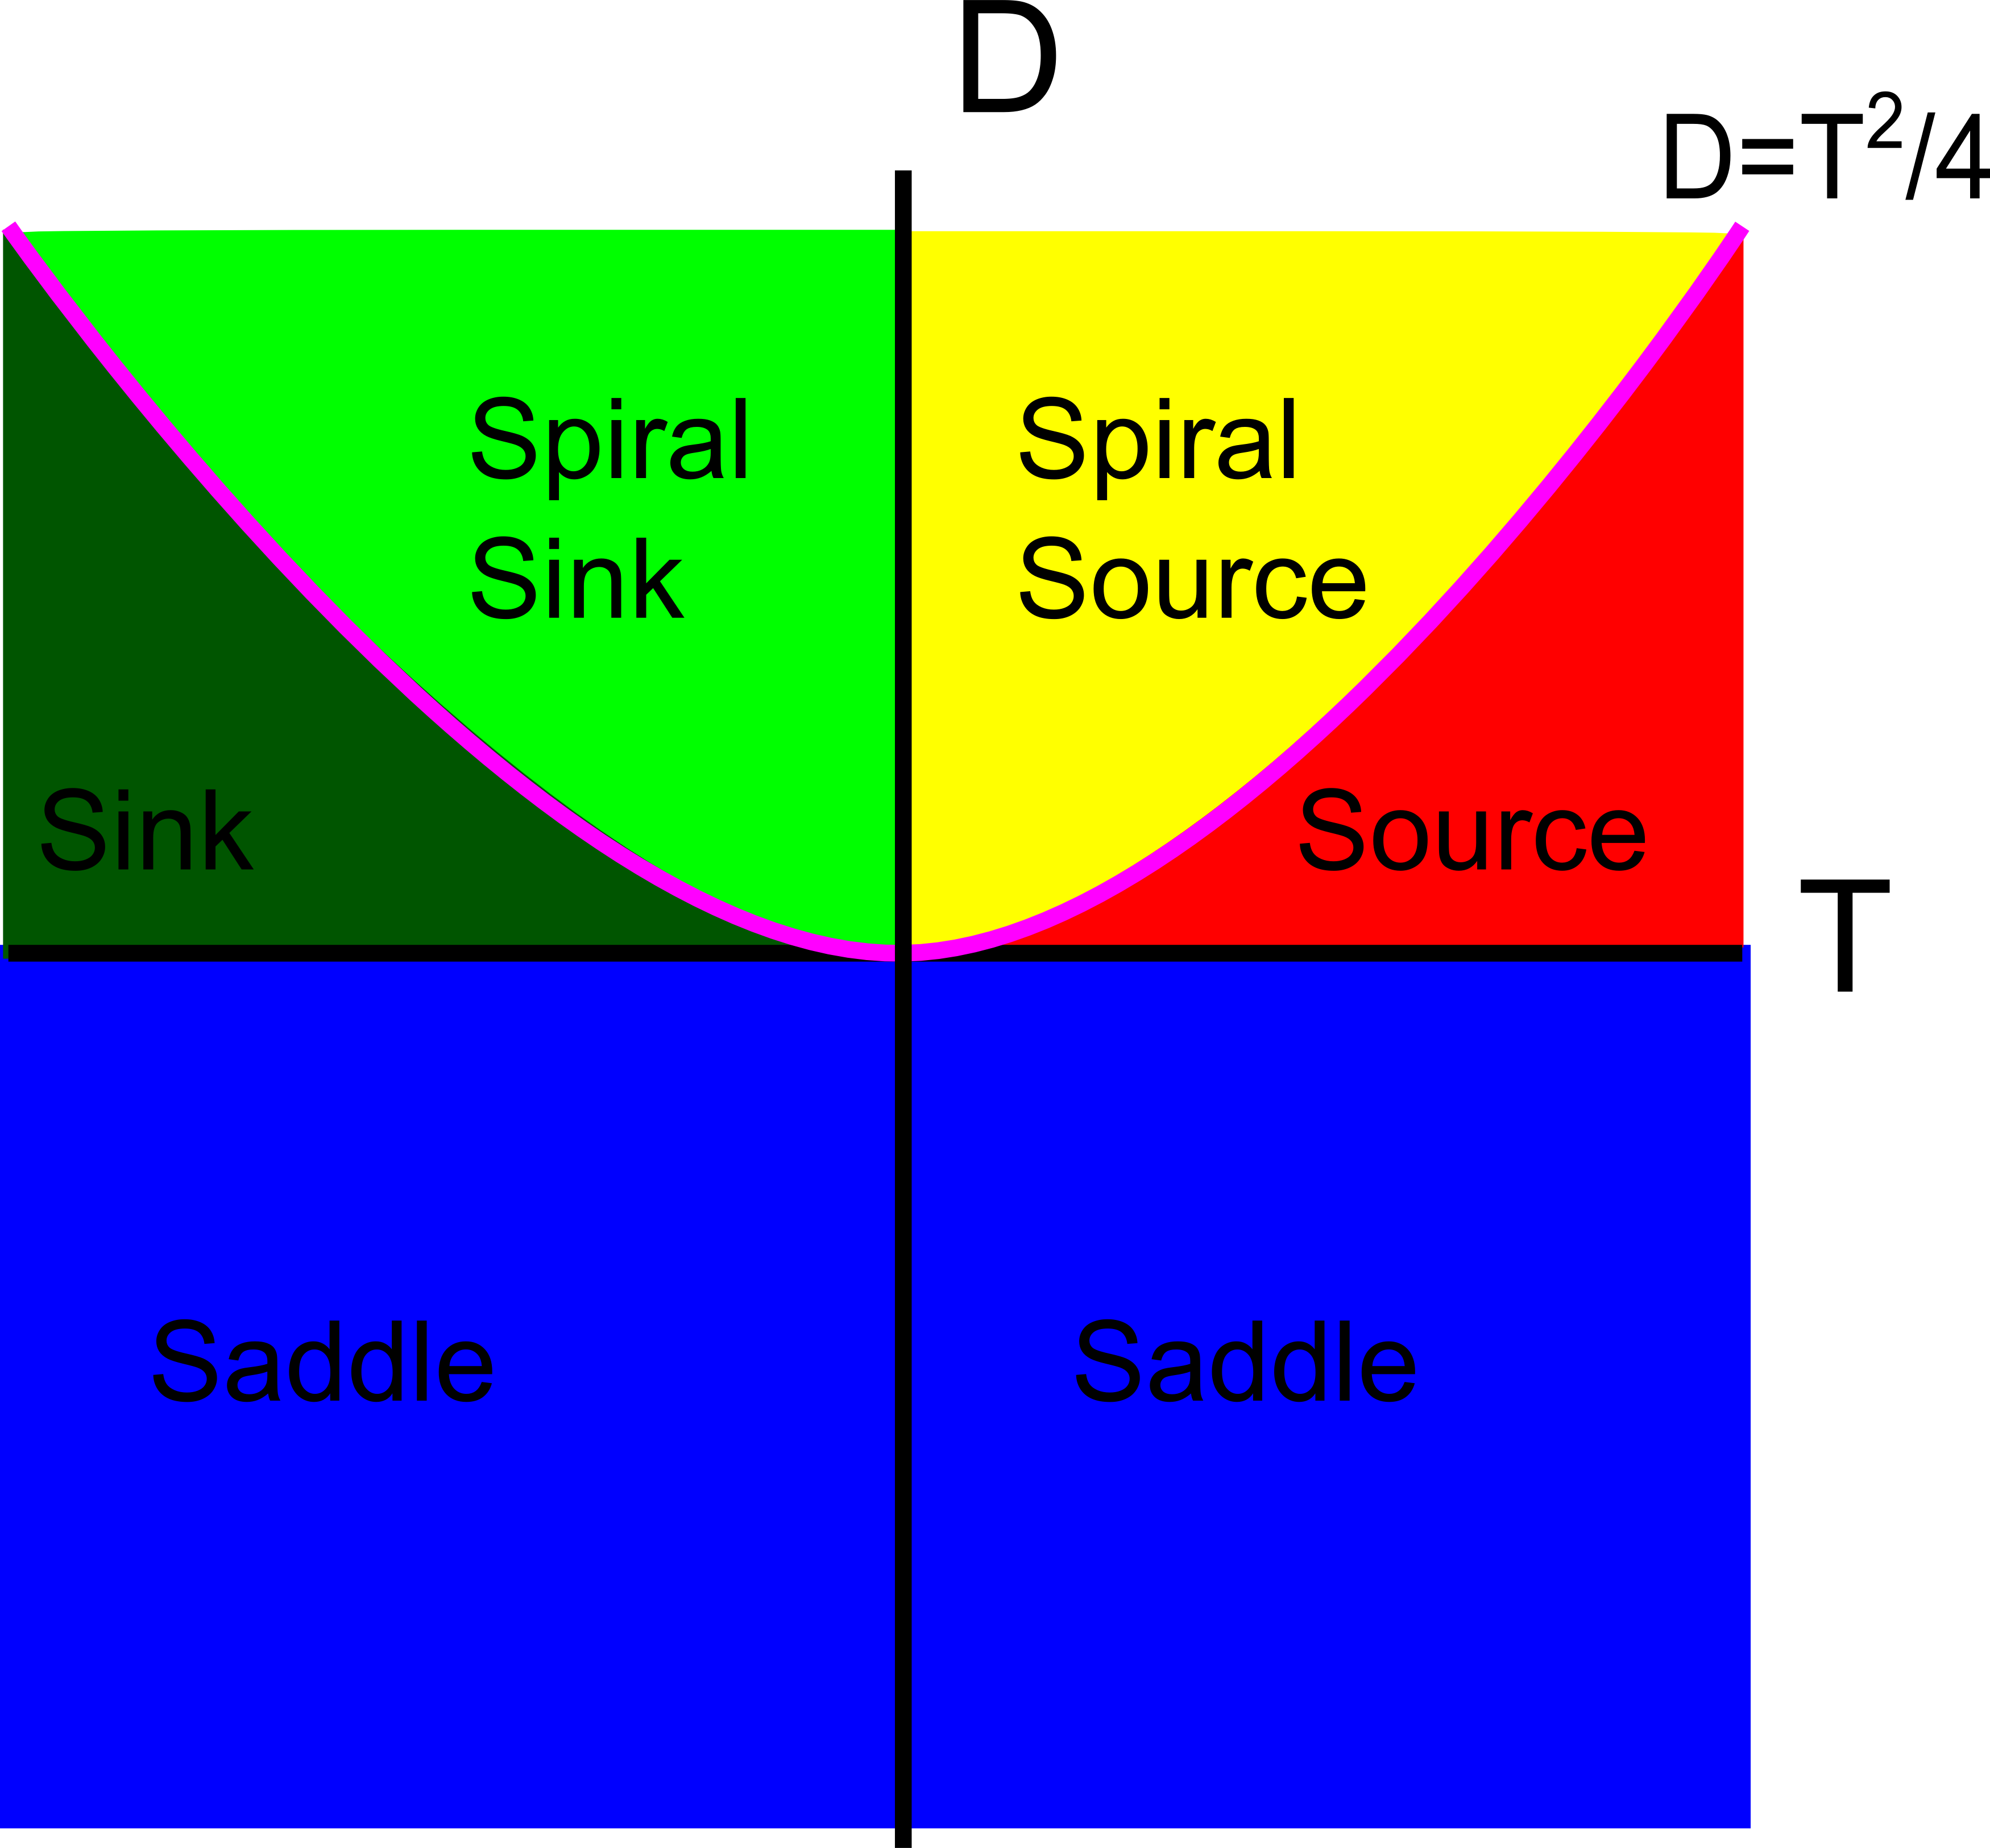
\includegraphics[width=5cm]{img/traceDeterminantAnnotated}}}
  
\end{frame}

\subsection{Examples}

\begin{frame}
  \frametitle{Example}

  \begin{eqnarray*}
    \deriv{~}{t} \vec{x} & = & \arrayTwo{2}{4}{1}{3} \vec{x}.
  \end{eqnarray*}

  \uncover<2->
  {
    \begin{eqnarray*}
      D & = & 2, \\
      T & = & 5.
    \end{eqnarray*}
  }

  \uncover<3->
  {
    \begin{eqnarray*}
      D & = & 2, \\
      D=2 & > & 0, \\
      D = 2 & < & \frac{25}{4} = \frac{T^2}{4}.
    \end{eqnarray*}
  }

  \uncover<4->
  {
    This is a source.
  }


\end{frame}


\iftoggle{clicker}{%
\begin{frame}
  \frametitle{Clicker Quiz}

   \ifnum\value{clickerQuiz}=1{%
   What are the values of $D$ and $T$ for the system of equations
   given by
   \begin{eqnarray*}
     \deriv{~}{t} \vec{x} & = & \arrayTwo{1}{4}{1}{3} \vec{x}?
   \end{eqnarray*}

     \begin{tabular}{ll}
       A: &   $D=7$, $T=4$ \\
       B: &   $D=-1$, $T=4$ \\
       C: &   $D=-1$, $T=3$ \\
     \end{tabular}

     \vfill


 }\fi

 \ifnum\value{clickerQuiz}=2{%
   What are the values of $D$ and $T$ for the system of equations
   given by
   \begin{eqnarray*}
     \deriv{~}{t} \vec{x} & = & \arrayTwo{1}{4}{1}{3} \vec{x}?
   \end{eqnarray*}

     \begin{tabular}{ll}
       A: &   $D=-1$, $T=3$ \\
       B: &   $D=-1$, $T=4$ \\
       C: &   $D=7$, $T=4$ \\
     \end{tabular}

     \vfill

 }\fi

 \ifnum\value{clickerQuiz}=3{%
  \vfill
 }\fi
\end{frame}
}


\begin{frame}
  \frametitle{Example}

  \begin{eqnarray*}
    \deriv{~}{t} \vec{x} & = & \arrayTwo{1}{4}{1}{3} \vec{x}.
  \end{eqnarray*}

\end{frame}


\begin{frame}
  \frametitle{Example}

  What is the behavior of
  \begin{eqnarray*}
    \deriv{~}{t} \vec{x} & = & \arrayTwo{1}{k}{1}{0} \vec{x}.
  \end{eqnarray*}
  for all values of $k$?

  \only<2-3>
  {
    \begin{eqnarray*}
      D & = & -k, \\
      T & = & 1.
    \end{eqnarray*}
  }



  \only<3>
  {
    Where is it a saddle?
    \begin{eqnarray*}
      D & = & -k \\
      -k & < & 0, \\ 
      k & > & 0.
    \end{eqnarray*}
    Saddle if $k>0$.
  }

  \only<4>
  {
    Where is it a source?
    \begin{eqnarray*}
      \begin{array}{rcccl}
        0 & < & D & < & \frac{T^2}{4}, \\
        0 & < & -k & < & \frac{1}{4}, \\\
        0 & > &  k & > & -\frac{1}{4}.
      \end{array}
    \end{eqnarray*}
    It is a source if $0 > k  > -\frac{1}{4}$.
  }

  \only<5>
  {
    Where is it a spiral source?
    \begin{eqnarray*}
        D  & > & \frac{T^2}{4}, \\
        -k & > & \frac{1}{4}, \\\
        k  & < & -\frac{1}{4}.
    \end{eqnarray*}
    It is a spiral source if $k < -\frac{1}{4}$.
  }

  \only<6->
  {
    \begin{tabular}{ll}
      saddle        & $k>0$\\
      source        & $0 > k  > -\frac{1}{4}$ \\
      spiral source & $k < -\frac{1}{4}$
    \end{tabular}
  }
  

\end{frame}


\begin{frame}
  \frametitle{Example}

  What is the behavior of
  \begin{eqnarray*}
    \deriv{~}{t} \vec{x} & = & \arrayTwo{-2}{k}{k}{0} \vec{x}.
  \end{eqnarray*}
  for all values of $k$?

  \only<2-3>
  {
    \begin{eqnarray*}
      D & = & -k^2, \\
      T & = & -2.
    \end{eqnarray*}
  }



  \only<3>
  {
    Where is it a saddle?
    \begin{eqnarray*}
      D & = & -k^2 \\
      -k^2 & < & 0, \\ 
    \end{eqnarray*}
    True for all $k\neq 0$.
  }


\end{frame}


\begin{frame}
  \frametitle{Example}

  What is the behavior of
  \begin{eqnarray*}
    \deriv{~}{t} \vec{x} & = & \arrayTwo{1}{k}{1}{-2} \vec{x}.
  \end{eqnarray*}
  for all values of $k$?

  \only<2-3>
  {
    \begin{eqnarray*}
      D & = & -2-k, \\
      T & = & -1.
    \end{eqnarray*}
  }



  \only<3>
  {
    Where is it a saddle?
    \begin{eqnarray*}
      D & = & -2-k \\
      -2-k & < & 0, \\ 
      k & > & -2.
    \end{eqnarray*}
    True for all $k>-2$.
  }


  \only<4>
  {
    Where is it a sink?
    \begin{eqnarray*}
      \begin{array}{rcccl}
        0 & < & D & < & \frac{T^2}{4}, \\
        0 & < & -2-k & < & \frac{4}{4}, \\\
        -2 & > &  k & > -3& .
      \end{array}
    \end{eqnarray*}
    It is a sink if $-2 > k  > -3$.
  }

  \only<5>
  {
    Where is it a spiral sink?
    \begin{eqnarray*}
        D  & > & \frac{T^2}{4}, \\
        -2-k & > & \frac{4}{4}, \\\
        k  & < & -3.
    \end{eqnarray*}
    It is a spiral sink if $k < -3$.
  }

  \only<6->
  {
    \begin{tabular}{ll}
      saddle        & $k>-2$\\
      source        & $-2 > k  > -3$ \\
      spiral sink   & $k < -3$
    \end{tabular}
  }



\end{frame}


\begin{frame}
  \frametitle{Example}

  What is the behavior of
  \begin{eqnarray*}
    \deriv{~}{t} \vec{x} & = & \arrayTwo{k}{2}{-1}{0} \vec{x}.
  \end{eqnarray*}
  for all values of $k$?


  \only<2-3>
  {
    \begin{eqnarray*}
      D & = & 2, \\
      T & = & k.
    \end{eqnarray*}
  }



  \only<3>
  {
    Where is it a sink/source?
    \begin{eqnarray*}
      D & < & \frac{T^2}{4}, \\
      2 & < & \frac{k^2}{4}, \\
      8 & < & k^2
    \end{eqnarray*}
    True for all $k^2>8$.
  }


  \only<4>
  {
    Where is it a sink?
    \begin{eqnarray*}
      k & < & -\sqrt{8}.
    \end{eqnarray*}
  }

  \only<5>
  {
    Where is it a spiral sink?
    \begin{eqnarray*}
      \begin{array}{rcccl}
        -\sqrt{8} < & T & < & 0, \\
        -\sqrt{8} < & k & < & 0. \\
      \end{array}
    \end{eqnarray*}
    It is a spiral sink if $-\sqrt{8}<k<0$.
  }

  \only<6>
  {
    Where is it a spiral source?
    \begin{eqnarray*}
      \begin{array}{rcccl}
        0 < & T & < & \sqrt{8}, \\
        0 < & k & < & \sqrt{8}.
      \end{array}
    \end{eqnarray*}
    It is a spiral source if $0<k<\sqrt{8}$.
  }

  \only<7>
  {
    Where is it a source?
    \begin{eqnarray*}
        T & > & \sqrt{8}, \\
        k & > & \sqrt{8}, \\
    \end{eqnarray*}
    It is a  source if $k>\sqrt{8}$.
  }


  \only<8->
  {
    \begin{tabular}{ll}
      sink          & $k>-\sqrt{8}$\\
      spiral sink   & $-\sqrt{8} < k < 0$ \\
      spiral source & $0 < k < \sqrt{8}$ \\
      source        & $k>\sqrt{8}$
    \end{tabular}
  }



\end{frame}




% LocalWords:  Clarkson pausesection hideothersubsections




% %%%%%%%%%%%%%%%%%%%%%%%%%%%%%%%%%%%%%%%%%%%%%%%%%%%%%%%%%%%%
% Laplace Transforms

\part{Partial-Fractions}
\lecture{Partial Fractions}{Partial-Fractions}
\section{Partial Fractions}


\title{Partial Fractions}
\subtitle{It Is Not Just For Integration Any More}
\date{14 November 2014}

\begin{frame}
  \titlepage
\end{frame}

\begin{frame}
  \frametitle{Outline}
  \tableofcontents[ currentsection ]
\end{frame}


\subsection{Test is Soon!}

\begin{frame}{Test on 18 November!}
  \centerline{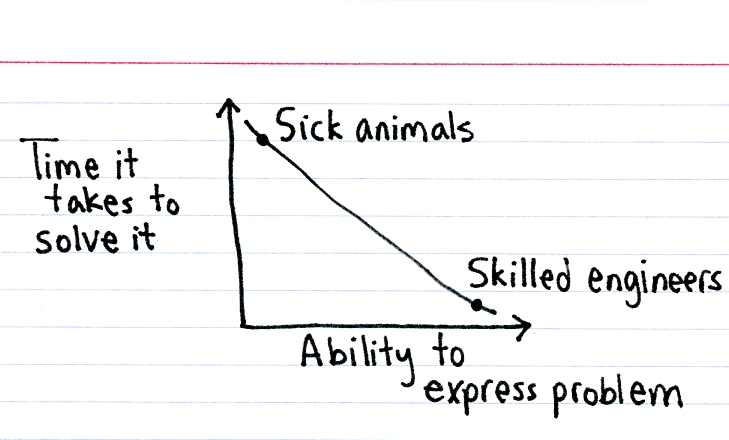
\includegraphics[width=5cm]{img/skilledEngineers}}

  {\tiny
    (from
    \url{http://thisisindexed.com/2013/10/just-tell-me-whats-the-matter/})
  }

  There is a reason why we stress how you approach a problem!

\end{frame}
\subsection{Partial Fractions}


\iftoggle{clicker}{%
\begin{frame}
  \frametitle{Clicker Quiz}

   \ifnum\value{clickerQuiz}=1{%
     What is the common denominator for
     \begin{eqnarray*}
       \frac{3}{7} + \frac{2}{3}?
     \end{eqnarray*}
     \begin{tabular}{ll}
       A: & $3$  \\ [12pt]
       B: & $7$  \\ [12pt]
       C: & $14$ \\ [12pt]
       D: & $21$ \\ [12pt]
     \end{tabular}

     \vfill
   }\fi

   \ifnum\value{clickerQuiz}=2{%
     What is the common denominator for
     \begin{eqnarray*}
       \frac{-1}{5} + \frac{7}{8}?
     \end{eqnarray*}
     \begin{tabular}{ll}
       A: & $5$  \\ [12pt]
       B: & $8$  \\ [12pt]
       C: & $40$ \\ [12pt]
       D: & $45$ \\ [12pt]
     \end{tabular}


   \vfill
   }\fi

  \ifnum\value{clickerQuiz}=3{%
    What is the common denominator for
     \begin{eqnarray*}
       \frac{-3}{7} + \frac{7}{8}?
     \end{eqnarray*}
     \begin{tabular}{ll}
       A: & $7$  \\ [12pt]
       B: & $8$  \\ [12pt]
       C: & $56$ \\ [12pt]
       D: & $24$ \\ [12pt]
     \end{tabular}

  \vfill
 }\fi
\end{frame}
}


\begin{frame}
  \frametitle{Partial Fractions}

  Appendix PF in your book.

  \uncover<2->
  {
    \begin{eqnarray*}
      \frac{6}{x-3} - \frac{4}{x-2} & = & 
      \uncover<3->
      {
        \frac{6\redText{(x-2)}}{\redText{(x-2)}(x-3)} - 
        \frac{4\blueText{(x-3)}}{(x-2)\blueText{(x-3)}}\\
        & = & \frac{2x}{x^2-5x+6}
      }
    \end{eqnarray*}
  }

\end{frame}


\begin{frame}
  \frametitle{Integration}

  We have 
  \begin{eqnarray*}
    \frac{6}{x-3} - \frac{4}{x-2} & = &  \frac{2x}{x^2-5x+6}.
  \end{eqnarray*}

  We can integrate
  \begin{eqnarray*}
    \int \frac{2x}{x^2-5x+6} ~ dx & = & \int \frac{6}{x-3} - \frac{4}{x-2} ~ dx, \\
    & = & 6\ln(x-3) - 4\ln(x-2) + C.
  \end{eqnarray*}

  \uncover<2->
  {
    \redText{Question: How do we do this backwards?}

    \blueText{Answer: Expand in terms of unknown coefficients and ``do the algebra.''}
  }

\end{frame}


\begin{frame}
  \frametitle{The Idea}

  We have the ratio of two polynomials, $\frac{p(x)}{q(x)}$:
  \begin{itemize}
  \item The degree of $p(x)$ is less than the degree of $q(x)$.
  \item Factor $q(x)$.
  \item Write out a general expansion in terms of the factors.
  \item Solve for unknown constants.
  \end{itemize}

\end{frame}

\subsection{Examples}

\begin{frame}
  \frametitle{Example}

  \begin{eqnarray*}
    \frac{2x}{x^2-5x+6} & = & 
    \uncover<2->
    {
      \frac{2x}{(x-3)(x-2)}, \\
      & = & \frac{\redText{a}}{x-3} + \frac{\blueText{b}}{x-2}.
    }
  \end{eqnarray*}

  \uncover<3->
  {
    Multiply both sides by $(x-3)(x-2)$:
    \begin{eqnarray*}
      \lefteqn{\frac{2x}{(x-3)(x-2)} \cdot (x-3)(x-2)  } \\
      & = & \lp \frac{\redText{a}}{x-3} + \frac{\blueText{b}}{x-2} \rp \cdot (x-3)(x-2), \\
      \uncover<4->
      {
        & = &  \frac{\redText{a}}{x-3} \cdot (x-3)(x-2) + 
               \frac{\blueText{b}}{x-2} \cdot (x-3)(x-2), \\
      }
      \uncover<5->
      {
        2x & = & \redText{a} (x-2) + \blueText{b}(x-3).
      }
    \end{eqnarray*}
  }


\end{frame}


\begin{frame}
  \frametitle{Solve for the Constants}
  \vspace*{-1em}
  We have:
  \begin{eqnarray*}
    2x & = & \redText{a} (x-2) + \blueText{b} (x-3).
  \end{eqnarray*}

  Let $x=2$:
  \begin{eqnarray*}
    2(2) & = & \redText{a} ((2)-2) + \blueText{b} ((2)-3) \\
    \Rightarrow 4 & = & -\blueText{b}.
  \end{eqnarray*}

  Let $x=3$:
  \begin{eqnarray*}
    2(3) & = & \redText{a} ((3)-2) + \blueText{b} ((3)-3) \\
    \Rightarrow 6 & = & \redText{a}.
  \end{eqnarray*}

  \uncover<2->
  {
    Substitute back into the original expansion:
    \begin{eqnarray*}
      \frac{2x}{x^2-5x+6} & = & \frac{6}{x-3} - \frac{4}{x-2}.
    \end{eqnarray*}
  }

\end{frame}


\begin{frame}
  \frametitle{Example}

  \begin{eqnarray*}
    \frac{5x}{x^2+4x-32} & = & \uncover<2->{ \frac{5x}{(x-4)(x+8) }} \\
    \uncover<3->{ & = & \frac{\redText{a}}{x-4} + \frac{\blueText{b}}{x+8} } \\
    \uncover<4->{ 5x & = & \redText{a} (x+8) + \blueText{b} (x-4).}
  \end{eqnarray*}

  \uncover<5->
  {
    Let $x=-8$:
    \begin{eqnarray*}
      -40 & = & -12\blueText{b}, \\
      \blueText{b} & = & \frac{10}{3}.
    \end{eqnarray*}

    Let $x=4$:
    \begin{eqnarray*}
      20 & = & 12\redText{a}, \\
      \redText{a}  & = & \frac{5}{3}.
    \end{eqnarray*}

  }


\end{frame}


\begin{frame}

    Substitute back in to get
    \begin{eqnarray*}
    \frac{5x}{x^2+4x-32} & = & \frac{5/3}{x-4} + \frac{10/3}{x+8} 
    \end{eqnarray*}


\end{frame}


\iftoggle{clicker}{%
\begin{frame}
  \frametitle{Clicker Quiz}

   \ifnum\value{clickerQuiz}=1{%
     What is the common denominator for
     \begin{eqnarray*}
       \frac{3}{x-5} + \frac{8}{(x-5)^2}?
     \end{eqnarray*}
     \begin{tabular}{ll}
       A: & $x-5$ \\ [12pt]
       B: & $(x-5)^2$ \\ [12pt]
       C: & $\ln(x-5)$ 
     \end{tabular}

     \vfill
   }\fi

   \ifnum\value{clickerQuiz}=2{%
     What is the common denominator for
     \begin{eqnarray*}
       \frac{-1}{x+7} + \frac{12}{(x+7)^2}?
     \end{eqnarray*}
     \begin{tabular}{ll}
       A: & $x+7$ \\ [12pt]
       B: & $(x+7)^2$ \\ [12pt]
       C: & $\ln(x+7)$ 
     \end{tabular}


   \vfill
   }\fi

  \ifnum\value{clickerQuiz}=3{%
     What is the common denominator for
     \begin{eqnarray*}
       \frac{-4}{x+9} + \frac{12}{(x+9)^2}?
     \end{eqnarray*}
     \begin{tabular}{ll}
       A: & $x+9$ \\ [12pt]
       B: & $(x+9)^2$ \\ [12pt]
       C: & $\ln(x+9)$
     \end{tabular}
 
  \vfill
 }\fi
\end{frame}
}


\begin{frame}
  \frametitle{Quadratic Terms}

  Note that
  \begin{eqnarray*}
    \frac{2}{x+2} + \frac{4}{(x+2)^2} & = & 
    \uncover<2->{%
          \frac{2\redText{(x+2)}}{(x+2)\redText{(x+2)}} + \frac{4}{(x+2)^2}, \\
        }
    \uncover<3->{%
      & = & \frac{2(x+2)+4}{(x+2)^2}, \\
      & = & \frac{2x+8}{x^2+4x+4}.
    }
  \end{eqnarray*}

\end{frame}


\begin{frame}
  \frametitle{Example}

  \begin{eqnarray*}
    \frac{2x+8}{x^2+4x+4} & = & \uncover<2->{ \frac{2x+8}{(x+2)^2}} \\
    \uncover<3->{ & = & \frac{\redText{a}}{x+2} + \frac{\blueText{b}}{(x+2)^2} } \\
    \uncover<4->{ 2x+8 & = & \redText{a} (x+2) + \blueText{b}.}
  \end{eqnarray*}

  \uncover<5->
  {
    Let $x=-2$:
    \begin{eqnarray*}
      4 & = & \blueText{b}.
    \end{eqnarray*}

    Let $x=0$:
    \begin{eqnarray*}
      8 & = & 2\redText{a}+\blueText{b}, \\
      a  & = & 2.
    \end{eqnarray*}

  }


\end{frame}


\begin{frame}

    Substitute back in to get
    \begin{eqnarray*}
    \frac{2x+8}{x^2+4x+4} & = & \frac{2}{x+2} + \frac{4}{(x+2)^2} 
    \end{eqnarray*}


\end{frame}


\begin{frame}
  \frametitle{Example}

  \begin{eqnarray*}
    \frac{3x+1}{x^2+6x+9} & = & \uncover<2->{ \frac{3x+1}{(x+3)^2}} \\
    \uncover<3->{ & = & \frac{\redText{a}}{x+3} + \frac{\blueText{b}}{(x+3)^2} } \\
    \uncover<4->{ 3x+1 & = & \redText{a} (x+3) + \blueText{b}.}
  \end{eqnarray*}

  \uncover<5->
  {
    Let $x=-3$:
    \begin{eqnarray*}
      -8 & = & \blueText{b}.
    \end{eqnarray*}

    Let $x=0$:
    \begin{eqnarray*}
      1 & = & 3\redText{a}+\blueText{b}, \\
      \redText{a}  & = & 3.
    \end{eqnarray*}

  }


\end{frame}


\begin{frame}

    Substitute back in to get
    \begin{eqnarray*}
    \frac{3x+1}{x^2+6x+9} & = & \frac{3}{x+3} - \frac{8}{(x+3)^2} 
    \end{eqnarray*}


\end{frame}


\begin{frame}
  \frametitle{Example}

  \begin{eqnarray*}
    \frac{4x^2+1}{x^3-3x^2-4x} & = & \uncover<2->{ \frac{4x^2+1}{x(x-4)(x+1)}} \\
    \uncover<3->{ & = & \frac{\redText{a}}{x} + \frac{\blueText{b}}{x-4} + 
      \frac{\fuchsiaText{c}}{x+1} } \\
    \uncover<4->{ 4x^2+1 & = & \redText{a} (x-4)(x+1) + \blueText{b}x(x+1) + \fuchsiaText{c}x(x-4).}
  \end{eqnarray*}

  \uncover<5->
  {
    Let $x=4$:
    \begin{eqnarray*}
      \blueText{b} & = & \frac{13}{4}.
    \end{eqnarray*}

    Let $x=-1$:
    \begin{eqnarray*}
      \fuchsiaText{c} & = & 1.
    \end{eqnarray*}

    Let $x=0$:
    \begin{eqnarray*}
      \redText{a} & = & \frac{-1}{4}.
    \end{eqnarray*}

  }


\end{frame}


\begin{frame}

    Substitute back in to get
    \begin{eqnarray*}
    \frac{4x^2+1}{x^3-3x^2-4x} & = & \frac{-1/4}{x} + \frac{13/4}{x-4} + \frac{1}{x+1}.
    \end{eqnarray*}


\end{frame}


\begin{frame}
  \frametitle{Example}

  \begin{eqnarray*}
    \frac{2x^2+3x-2}{x^3-3x+2} & = & \uncover<2->{ \frac{2x^2+3x-2}{(x-1)^2(x+2)}} \\
    \uncover<3->{ & = & \frac{\redText{a}}{x-1} + 
                        \frac{\blueText{b}}{(x-1)^2} + 
                        \frac{\fuchsiaText{c}}{x+2} } \\
    \uncover<4->{ 2x^2+3x-2 & = & a (x-1)(x+2) + b(x+2) + c(x-1)^2.}
  \end{eqnarray*}

  \uncover<5->
  {
    Let $x=1$:
    \begin{eqnarray*}
      \blueText{b} & = & 1.
    \end{eqnarray*}

    Let $x=-2$:
    \begin{eqnarray*}
      \fuchsiaText{c} & = & 0.
    \end{eqnarray*}

    Let $x=0$:
    \begin{eqnarray*}
      \redText{a} & = & 2.
    \end{eqnarray*}

  }


\end{frame}


\begin{frame}

    Substitute back in to get
    \begin{eqnarray*}
    \frac{2x^2+3x-2}{x^3-3x+2} & = & \frac{2}{x-1} + \frac{1}{(x-1)^2}.
    \end{eqnarray*}


\end{frame}


\begin{frame}
  \frametitle{More Quadratics}

  \begin{eqnarray*}
    \frac{x+3}{x^2+x+4} - \frac{1}{x-2} & = & 
    \frac{(x+3)\redText{(x-2)}}{(x^2+x+4)\redText{(x-2)}} - 
    \frac{\blueText{(x^2+x+4)}}{(x-2)\blueText{(x^2+x+4)}}, \\
    & = & \frac{x^2+x-6-(x^2+x+4)}{(x-2)(x^2+x+4)}, \\
    & = & \frac{-10}{(x-2)(x^2+x+4)}. \\
  \end{eqnarray*}

\end{frame}

\begin{frame}
  \frametitle{Working It Backwards}
  
  Given
  \begin{eqnarray*}
    \frac{-10}{(x-2)(x^2+x+4)} & = & \frac{\redText{a}}{x-2} + 
                                     \frac{\blueText{b}x+\fuchsiaText{c}}{x^2+x+4}, \\
    \Rightarrow -10 & = & \redText{a}(x^2+x+4) + (\blueText{b}x+\fuchsiaText{c})(x-2).
  \end{eqnarray*}

  \uncover<2->
  {
    Let $x=2$:
    \begin{eqnarray*}
      \redText{a} & = & -1.
    \end{eqnarray*}

    %%%%%%%%%%%%%%%%%%%%
    Let $x=0$:
    \begin{eqnarray*}
      \fuchsiaText{c} & = & 3.
    \end{eqnarray*}
 
    Let $x=1$:
    \begin{eqnarray*}
      \blueText{b} & = & 1.
    \end{eqnarray*}

    Substitute back in to get
    \begin{eqnarray*}
     \frac{-10}{(x-2)(x^2+x+4)}= \frac{-1}{x-2} + \frac{x+3}{x^2+x+4}. 
  \end{eqnarray*}

    %Match the polynomial terms:
    %\begin{eqnarray*}
    %  -10 & = & -(x^2+x+4) + (bx+c)(x-2), \\
    %  -10 & = & -x^2 - x - 4 + bx^2 - 2bx + cx - 2c, \\
    %  \Rightarrow b & = & 1, \\
    %  c & = & 3.
    %\end{eqnarray*}
  }

\end{frame}


\begin{frame}
  \frametitle{General Forms}

  \begin{eqnarray*}
    \frac{1}{x^3+1} & = & \frac{1}{(x+1)(x^2-x+1)}= \frac{a}{x+1} + \frac{bx+c}{x^2-x+1}.
  \end{eqnarray*}

  \begin{eqnarray*}
    \frac{5}{(x^2+4)(x^2-x+10)} & = & \frac{ax+b}{x^2+4} + \frac{cx+d}{x^2-x+10}.
  \end{eqnarray*}

  \begin{eqnarray*}
    \frac{18}{(x-1)(x+2)(x+3)} & = & \frac{a}{x-1} + \frac{b}{x+2} + \frac{c}{x+3}.
  \end{eqnarray*}


  \begin{eqnarray*}
    \frac{4}{x^2(3x^2+2)} & = & \frac{a}{x} + \frac{b}{x^2} + \frac{cx+d}{3x^2+2}.
  \end{eqnarray*}

  \begin{eqnarray*}
    \frac{4}{x^2(3x^2-2)} & = & \frac{a}{x} + \frac{b}{x^2} + \frac{c}{x+\sqrt{\frac{2}{3}}} + \frac{d}{x-\sqrt{\frac{2}{3}}}.
  \end{eqnarray*}

  
\end{frame}



% LocalWords:  Clarkson pausesection hideothersubsections

\part{Laplace-Transforms}
\lecture{Laplace Transforms}{Laplace-Transforms}
\section{Laplace Transforms}


\title{Ordinary Differential Equations}
\subtitle{Math 232 - Week 12, Day 2}
\date{14 November 2012}

\begin{frame}
  \titlepage
\end{frame}

\begin{frame}
  \frametitle{Outline}
  \tableofcontents[ currentsection ]
\end{frame}


\subsection{Laplace Transform}


\begin{frame}
  \frametitle{Example}

  \begin{eqnarray*}
    \int^\infty_0 e^{-3t} ~ dt & = & 
    \uncover<2->
    {%
      \lim_{M\rightarrow\infty} -\frac{1}{3} e^{-3t} \bigg|^M_0, \\
      & = & \frac{1}{3}.
    }
  \end{eqnarray*}

\end{frame}


\iftoggle{clicker}{%
\begin{frame}
  \frametitle{Clicker Quiz}

   \ifnum\value{clickerQuiz}=1{%
     Is the integral 
     \begin{eqnarray*}
       \int^\infty_0 e^{-7t} ~ dt
     \end{eqnarray*}
     a function of time?

     \vspace{2em}
     \begin{tabular}{ll}
       A: & Yes \\ [12pt]
       B: & No
     \end{tabular}

     \vfill
   }\fi

   \ifnum\value{clickerQuiz}=2{%
     Is the integral 
     \begin{eqnarray*}
       \int^\infty_0 e^{-2t} ~ dt
     \end{eqnarray*}
     a function of time?

     \vspace{2em}
     \begin{tabular}{ll}
       A: & Yes \\ [12pt]
       B: & No
     \end{tabular}

   \vfill
   }\fi

  \ifnum\value{clickerQuiz}=3{%
     Is the integral
     \begin{eqnarray*}
       \int^\infty_0 e^{-5t} ~ dt
     \end{eqnarray*}
     a function of time?

     \vspace{2em}
     \begin{tabular}{ll}
       A: & Yes \\ [12pt]
       B: & No
     \end{tabular}


  \vfill
 }\fi
\end{frame}
}


\begin{frame}
  \frametitle{Example}

  \begin{eqnarray*}
    \int^\infty_0 e^{-st} ~ dt & = & 
    \uncover<2->
    {%
      \lim_{M\rightarrow\infty} -\frac{1}{s} e^{-st} \bigg|^M_0, \\
      & = & \frac{1}{s}
    }
  \end{eqnarray*}
  (Assume that $s>0$.)

  \uncover<3->
  {%
    Note that this is not a function of $t$. 
  }
  

\end{frame}


\begin{frame}
  \frametitle{Laplace Transform}


  \begin{definition}
    The Laplace Transform of a function, $f(t)$, is 
    \begin{eqnarray*}
      \laplace{f} & = & F(s), \\
      & = & \int^\infty_0 f(t) e^{-st} ~ dt.
    \end{eqnarray*}
    \textit{(If it exists.)}
  \end{definition}

  \uncover<2->
  {%
    It will turn out that this is useful for solving differential
    equations because integrals ``undo'' derivatives. The goal is to
    turn a calculus problem into an algebra problem.
  }

\end{frame}


\iftoggle{clicker}{%
\begin{frame}
  \frametitle{Clicker Quiz}

   \ifnum\value{clickerQuiz}=1{%
     Is the the Laplace Transform 
     \begin{eqnarray*}
       F(s) & = & \int^\infty_0 f(t) e^{-st} ~ dt
     \end{eqnarray*}
     a function of time?

     \vspace{2em}
     \begin{tabular}{ll}
       A: & Yes \\ [12pt]
       B: & No
     \end{tabular}

     \vfill
   }\fi

   \ifnum\value{clickerQuiz}=2{%
     Is the the Laplace Transform 
     \begin{eqnarray*}
       F(s) & = & \int^\infty_0 f(t) e^{-st} ~ dt
     \end{eqnarray*}
     a function of time?

     \vspace{2em}
     \begin{tabular}{ll}
       A: & Yes \\ [12pt]
       B: & No
     \end{tabular}

   \vfill
   }\fi

  \ifnum\value{clickerQuiz}=3{%
      Is the the Laplace Transform
     \begin{eqnarray*}
       F(s) & = & \int^\infty_0 f(t) e^{-st} ~ dt
     \end{eqnarray*}
     a function of time?

     \vspace{2em}
     \begin{tabular}{ll}
       A: & Yes \\ [12pt]
       B: & No
     \end{tabular}


  \vfill
 }\fi
\end{frame}
}


\begin{frame}
  \frametitle{Properties of the Laplace Transform}

  The Laplace transform of the sum:
  \begin{eqnarray*}
    \laplace{f+g} & = & \int^\infty_0 \lp f(t) + g(t) \rp e^{-st} ~ dt, \\
    & = & \int^\infty_0 f(t) e^{-st} ~ dt + \int^\infty_0 g(t) e^{-st} ~ dt, \\
    & = & \laplace{f} + \laplace{g}.
  \end{eqnarray*}

  
  The Laplace transform of a constant times the function. Suppose $a$ is a constant, then
  \begin{eqnarray*}
    \laplace{a f} & = & \int^\infty_0 a f(t) e^{-st} ~ dt, \\
    & = & a \int^\infty_0 f(t) e^{-st} ~ dt, \\
    & = & a \laplace{f}.
  \end{eqnarray*}


\end{frame}


\begin{frame}
  \frametitle{So What?}

  If we have the Laplace transform of a function, 
  \begin{eqnarray*}
    \laplace{f} & = & F(s),
  \end{eqnarray*}
  then given $F(s)$ we can find $f(t)$. (We will do that later.) More
  importantly, integrals can ``get rid of'' derivatives.

\end{frame}

\subsection{Laplace Transforms of Polynomials}

\begin{frame}
  \frametitle{Laplace Transforms of Polynomials}

  \begin{eqnarray*}
    \begin{array}{rcl@{\hspace{1em}}c@{\hspace{1em}}l}
    \laplace{1} & = & \int^\infty_0 1 \cdot e^{-st} ~ dt
    & = & \frac{1}{s}, \\ [10pt]
    \laplace{t} & = & \int^\infty_0 t \cdot e^{-st} ~ dt
    & = & \frac{1}{s^2}, \\ [10pt]
    \laplace{t^2} & = & \int^\infty_0 t^2 \cdot e^{-st} ~ dt
    & = & \frac{2}{s^3}.      
    \end{array}
  \end{eqnarray*}

  \uncover<2->
  {%
    We can build up tables of these identities. It is then an issue of
    finding the right function in the table.
  }

\end{frame}


\begin{frame}
  \frametitle{Example}

  Find the Laplace transform of 
  \begin{eqnarray*}
    f(t) & = & \redText{3} + \blueText{5t} - \fuchsiaText{8t^2}.
  \end{eqnarray*}

  \uncover<2->
  {
    
    The Laplace transform is
    \begin{eqnarray*}
      \laplace{f} & = & \redText{\frac{3}{s}} + \blueText{\frac{5}{s^2}} - \fuchsiaText{\frac{16}{s^3}}.
    \end{eqnarray*}

  }

\end{frame}

\iftoggle{clicker}{%
\begin{frame}
  \frametitle{Clicker Quiz}

   \ifnum\value{clickerQuiz}=1{%

     \vfill
   }\fi

   \ifnum\value{clickerQuiz}=2{%

   \vfill
   }\fi

  \ifnum\value{clickerQuiz}=3{%
    Find the Laplace transform of
    \begin{eqnarray*}
      f(t) & = & 4 - 3t + 7t^2.
    \end{eqnarray*}

     \begin{tabular}{ll}
       A: & $\laplace{f} = \frac{4}{s} - \frac{3}{s^2} + \frac{14}{s^3}.$\\ [12pt]
       B: & $\laplace{f} = 4 - \frac{3}{s} + \frac{14}{s^2}.$\\ [12pt]
       C: & $\laplace{f} = \frac{4}{s} - \frac{3}{s^2} + \frac{7}{s^3}.$\\ [12pt]
     \end{tabular}

  \vfill
 }\fi
\end{frame}
}


\begin{frame}
  \frametitle{Example}

  Find the Laplace transform of 
  \begin{eqnarray*}
    f(t) & = & \redText{4} - \blueText{3t} + \fuchsiaText{7t^2}.
  \end{eqnarray*}

  \uncover<2->
  {

    The Laplace transform is
    \begin{eqnarray*}
      \laplace{f} & = & \redText{\frac{4}{s}} - \blueText{\frac{3}{s^2}} + \fuchsiaText{\frac{14}{s^3}}.
    \end{eqnarray*}

  }

\end{frame}


\begin{frame}
  \frametitle{Laplace Transform of Higher Order Polynomials}

  In general we have
  \begin{eqnarray*}
    \laplace{t^n} & = & \frac{n!}{s^{n+1}}.
  \end{eqnarray*}

\end{frame}


\begin{frame}
  \frametitle{Example}

  Find the Laplace transform of 
  \begin{eqnarray*}
    f(t) & = & \redText{5 t^3} - \blueText{17 t^5}.
  \end{eqnarray*}

  \uncover<2->
  {

    The Laplace transform is
    \begin{eqnarray*}
      \laplace{f} & = & \redText{5 \frac{3!}{s^4}} - \blueText{17 \frac{5!}{s^6}}.
    \end{eqnarray*}

  }

\end{frame}


%\iftoggle{clicker}{%
%\begin{frame}
%  \frametitle{Clicker Quiz}
%
%   \ifnum\value{clickerQuiz}=1{%
%
%     What is the Laplace transform of $f(t)=3t-4$?
%
%     \begin{tabular}{ll}
%       A: & $\frac{1}{s^2}-\frac{1}{s}$ \\ [12pt]
%       B: & $\frac{6}{s^2}-\frac{4}{s}$ \\ [12pt]
%       C: & $\frac{3}{s^2}-\frac{4}{s}$ 
%     \end{tabular}
%
%     \vfill
%   }\fi
%
%   \ifnum\value{clickerQuiz}=2{%
%
%     What is the Laplace transform of $f(t)=2t-6$?
%
%     \begin{tabular}{ll}
%       A: & $\frac{1}{s^2}-\frac{1}{s}$ \\ [12pt]
%       B: & $\frac{2}{s^2}-\frac{6}{s}$ \\ [12pt]
%       C: & $\frac{4}{s^2}-\frac{6}{s}$ 
%     \end{tabular}
%
%   \vfill
%   }\fi
%
%  \ifnum\value{clickerQuiz}=3{%
%    
%     What is the Laplace transform of $f(t)=6t-3$?
%
%     \begin{tabular}{ll}
%       A: & $\frac{6}{s^2}-\frac{1}{s}$ \\ [12pt]
%       B: & $\frac{12}{s^2}-\frac{3}{s}$ \\ [12pt]
%       C: & $\frac{6}{s^2}-\frac{3}{s}$
%     \end{tabular}
%
%  \vfill
% }\fi
%\end{frame}
%}

\subsection{Laplace Transform of Exponentials}

\begin{frame}
  \frametitle{Laplace Transform of Exponentials}

  \begin{eqnarray*}
    \laplace{e^{at}} & = & \int^\infty_0 e^{at} e^{-st} ~ dt, \\
    & = & \int^\infty_0 e^{(a-s)t} ~ dt, \\
    \Rightarrow \laplace{e^{at}} & = & \frac{1}{s-a}.
  \end{eqnarray*}

\end{frame}


\begin{frame}
  \frametitle{Example}

  Find the Laplace transform of 
  \begin{eqnarray*}
    f(t) & = & e^{3t}.
  \end{eqnarray*}

  \uncover<2->
  {
    
    The Laplace transform is
    \begin{eqnarray*}
      \laplace{f} & = & \frac{1}{s-3}.
    \end{eqnarray*}

  }

  \uncover<3->
  {
    Find the Laplace transform of 
    \begin{eqnarray*}
      g(t) & = & e^{-5t}.
    \end{eqnarray*}

  }

  \uncover<4->
  {
    The Laplace transform is
    \begin{eqnarray*}
      \laplace{g} & = & \frac{1}{s+5}.
    \end{eqnarray*}
  }


\end{frame}

\iftoggle{clicker}{%
\begin{frame}
  \frametitle{Clicker Quiz}

   \ifnum\value{clickerQuiz}=1{%

     \vfill
   }\fi

   \ifnum\value{clickerQuiz}=2{%


   \vfill
   }\fi

  \ifnum\value{clickerQuiz}=3{%
  Find the Laplace transform of
  \begin{eqnarray*}
    f(t) & = & 4t^2 - 18 e^{-6t}.
  \end{eqnarray*}
   \begin{tabular}{ll}
       A: & $ \laplace{f} = 4 \frac{2!}{s^3} - 18 \frac{1}{s-6}.$ \\ [12pt]
       B: & $ \laplace{f} = 4 \frac{1}{s^2} - 18 \frac{1}{s+6}.$ \\ [12pt]
       C: & $ \laplace{f} = 4 \frac{2!}{s^3} - 18 \frac{1}{s+6}.$ \\ [12pt]
     \end{tabular}

  \vfill
 }\fi
\end{frame}
}

\begin{frame}
  \frametitle{Example}

  Find the Laplace transform of 
  \begin{eqnarray*}
    f(t) & = & \redText{4t^2} - \blueText{18 e^{-6t}}.
  \end{eqnarray*}

  \uncover<2->
  {

    The Laplace transform is
    \begin{eqnarray*}
      \laplace{f} & = & \redText{4 \frac{2!}{s^3}} - \blueText{18 \frac{1}{s+6}}.
    \end{eqnarray*}

  }

\end{frame}


\iftoggle{clicker}{%
\begin{frame}
  \frametitle{Clicker Quiz}

   \ifnum\value{clickerQuiz}=1{%

     What is the Laplace transform of $f(t)=i$?

     \begin{tabular}{ll}
       A: & $\frac{1}{s}$ \\ [12pt]
       B: & $\frac{i}{s}$ \\ [12pt]
       C: & $\frac{i}{s^2}$ \\ [12pt]
       D: & Not possible
     \end{tabular}

     \vfill
   }\fi

   \ifnum\value{clickerQuiz}=2{%

     What is the Laplace transform of $f(t)=i$?

     \begin{tabular}{ll}
       A: & $\frac{1}{s}$ \\ [12pt]
       B: & $\frac{i}{s}$ \\ [12pt]
       C: & $\frac{i}{s^2}$ \\ [12pt]
       D: & Not possible
     \end{tabular}

   \vfill
   }\fi

  \ifnum\value{clickerQuiz}=3{%
     What is the Laplace transform of $f(t)=i$?

     \begin{tabular}{ll}
       A: & $\frac{1}{s}$ \\ [12pt]
       B: & $\frac{i}{s}$ \\ [12pt]
       C: & $\frac{i}{s^2}$ \\ [12pt]
       D: & Not possible
     \end{tabular}

  \vfill
 }\fi
\end{frame}
}


\subsection{Laplace Transform of Sines and Cosines}

\begin{frame}
  \frametitle{Sines and Cosines}

  Note that
  \begin{eqnarray*}
    \laplace{e^{iat}} & = & \frac{1}{s-ai}, \\
    & = & \frac{s+ai}{(s-ai)(s+ai)}, \\
    & = & \frac{s+ai}{s^2+a^2}, \\
    \only<2>{& = & \frac{s}{s^2+a^2} + i \frac{a}{s^2+a^2}. \\}
    \uncover<3->{& = & \redText{\frac{s}{s^2+a^2}} + i \blueText{\frac{a}{s^2+a^2}}.}
  \end{eqnarray*}


  \uncover<4->
  {

    At the same time, though,
    \begin{eqnarray*}
      \laplace{e^{iat}} & = & \laplace{\cos(at) + i \sin(at)}, \\
      & = & \redText{\laplace{\cos(at)}} + i \blueText{\laplace{\sin(at)}}.
    \end{eqnarray*}

  }


\end{frame}


\begin{frame}
  \frametitle{Sines and Cosines}

  The Laplace transform of the sine and cosine is the following:
  \begin{eqnarray*}
    \laplace{\cos(at)} & = & \frac{s}{s^2+a^2}, \\
    \laplace{\sin(at)} & = & \frac{a}{s^2+a^2}.
  \end{eqnarray*}


\end{frame}


\begin{frame}
  \frametitle{Example}

  Find the Laplace transform of 
  \begin{eqnarray*}
    f(t) & = & \redText{5t^4} + \blueText{2\sin(4t)} - \fuchsiaText{3 e^{8t}} + 7 \cos(5t).
  \end{eqnarray*}

  \uncover<2->
  {

    The Laplace transform is
    \begin{eqnarray*}
      \laplace{f} & = & \redText{5 \frac{4!}{s^5}} + \blueText{2 \frac{4}{s^2+16}}  - \fuchsiaText{3\frac{1}{s-8}} + 7 \frac{s}{s^2+25}.
    \end{eqnarray*}

  }

\end{frame}

\subsection{More Identities}

\begin{frame}
  \frametitle{More Identities}

  \begin{eqnarray*}
    \laplace{t f(t)} & = & \int^\infty_0 t f(t) e^{-st} ~ dt, \\
    & = & \int^\infty_0 f(t) \lp -\deriv{~}{s} e^{-st} \rp ~ dt, \\
    & = & -\deriv{~}{s} \int^\infty_0 f(t) e^{-st}  ~ dt, \\
    & = & -\deriv{~}{s} \laplace{f}(s).
  \end{eqnarray*}

\end{frame}

\begin{frame}
  \frametitle{Moar Moar Identities!}
  \begin{columns}
    \column{.5\textwidth} 
    \includegraphics[height=4cm]{img/cagemoar}


    \column{.5\textwidth}
    \begin{eqnarray*}
      \laplace{t^2 f(t)} & = & \frac{d^2}{ds^2} \laplace{f}, \\
      \uncover<2->
      {
        \laplace{t^3 f(t)} & = & -\frac{d^3}{ds^3} \laplace{f}, \\
      }
      \uncover<3->
      {
        \vdots             &   & \vdots \\
        \laplace{t^n f(t)} & = & (-1)^n \frac{d^n}{ds^n} \laplace{f}.
      }
    \end{eqnarray*}
  \end{columns}
  
\end{frame}


\begin{frame}
  \frametitle{Example}
    \begin{eqnarray*}
      f(t) & = & \redText{7t \sin(4t)} + \blueText{2t^3e^{-4t}}, \\
      \uncover<2->
      {
        \laplace{f} & = &- \redText{\deriv{~}{s} \frac{28}{s^2+16}} \blueText{- \frac{d^3}{ds^3} \frac{2}{(s+4)}}, \\
         & = & \redText{\frac{56s}{\lp s^2+16\rp^2}} + \blueText{12 \frac{1}{(s+4)^4}}.
      }
    \end{eqnarray*}
\end{frame}

\begin{frame}
  \frametitle{Moar Moar Moar Identities!}
  \begin{columns}
    \column{.1\textwidth} 
    \includegraphics[height=4cm]{img/moar_18}


    \column{.9\textwidth}
    \begin{eqnarray*}
      \laplace{e^{at} f(t)} & = & \int^\infty_0 e^{at} f(t) e^{-st} ~ dt, \\
      \uncover<2->
      {
        & = & \int^\infty_0 f(t) e^{-(s-a)t} ~ dt, \\
      }
      \uncover<3->
      {
        & = & \laplace{f}(s-a).
      }
    \end{eqnarray*}
  \end{columns}
  
\end{frame}


\iftoggle{clicker}{%
\begin{frame}
  \frametitle{Clicker Quiz}

   \ifnum\value{clickerQuiz}=1{%

     Was that Billy Idol?

     \begin{tabular}{ll}
       A: & Yes \\ [12pt]
       B: & Who? \\ [12pt]
       C: & No, that would be lame.
     \end{tabular}

     \vfill
   }\fi

   \ifnum\value{clickerQuiz}=2{%

     Was that Billy Idol?

     \begin{tabular}{ll}
       A: & Yes \\ [12pt]
       B: & Who? \\ [12pt]
       C: & No, that would be lame.
     \end{tabular}


   \vfill
   }\fi

  \ifnum\value{clickerQuiz}=3{%
    Was that Billy Idol?

     \begin{tabular}{ll}
       A: & Yes \\ [12pt]
       B: & Who? \\ [12pt]
       C: & No, that would be lame.
     \end{tabular}

  \vfill
 }\fi
\end{frame}
}


\begin{frame}
  \frametitle{Example}
    \begin{eqnarray*}
      f(t) & = & \redText{3t^4 e^{2t}} - \blueText{4 e^{-5t}\sin(3t)}, \\
      \uncover<2->
      {
        \laplace{f} & = & \redText{3 \laplace{t^4}(s-2)} - \blueText{4 \laplace{\sin(3t)}(s+5)}, \\
      }
      \uncover<3->
      {
        & = & \redText{3 \frac{4!}{(s-2)^5}} - \blueText{4 \frac{3}{(s+5)^2+9}}.
      }
    \end{eqnarray*}
\end{frame}


\begin{frame}
  \frametitle{Example}
    \begin{eqnarray*}
      f(t) & = & \redText{2 e^{-4t}\cos(3t)} - \blueText{5 t^2 \sin(2t)}, \\
      \uncover<2->
      {
        \laplace{f} & = & \redText{3 \laplace{\cos(3t)}(s+4)} - \blueText{5 (-1)^2 \frac{d^2}{ds^2} \laplace{\sin(2t)}}, \\
      }
      \uncover<3->
      {
        & = & \redText{2 \frac{s+4}{(s+4)^2+9}} + \blueText{20 \lp -8(s^2+4)^{-3}s^2 + (s^2+4)^{-2} \rp}.
      }
    \end{eqnarray*}
\end{frame}


\begin{frame}
  \frametitle{Oh By The Way....}

  \begin{definition}[The hyperbolic sine and hyperbolic cosine:]
    \begin{eqnarray*}
      \sinh(t) & = & \frac{e^t-e^{-t}}{2}, \\
      \cosh(t) & = & \frac{e^t+e^{-t}}{2}.
    \end{eqnarray*}
  \end{definition}

  \uncover<2->
  {
    Why? Because it makes other things easier.
    \begin{eqnarray*}
      \deriv{~}{t} \cosh(t) & = & \sinh(t), \\
      \deriv{~}{t} \sinh(t) & = & \cosh(t).
    \end{eqnarray*}
    (Think about solutions to DEs!)
  }

  
\end{frame}


\begin{frame}
  \frametitle{Oh By The Way....}

  It makes dealing with the inverse Laplace Transform much easier in some cases:
  \begin{eqnarray*}
    \laplace{\sinh(at)} & = & \frac{a}{s^2-a^2}, \\
    \laplace{\cosh(at)} & = & \frac{s}{s^2-a^2}.
  \end{eqnarray*}

  (We will see why soon.)

  But mostly it is because \textbf{some engineers like to use it}. You
  have to be prepared to come across this in the future.
  
\end{frame}



% LocalWords:  Clarkson pausesection hideothersubsections

\part{Inverse-Laplace-Transforms}
\lecture{Inverse Laplace Transforms}{Inverse-Laplace-Transforms}
\section{Inverse Laplace Transforms}


\title{Ordinary Differential Equations}
\subtitle{Math 232 - Week 12, Day 2}
\date{14 November 2012}

\begin{frame}
  \titlepage
\end{frame}

\begin{frame}
  \frametitle{Outline}
  \tableofcontents[pausesection,hideothersubsections]
\end{frame}


\subsection{Laplace Transform Table}

\begin{frame}
  \frametitle{Backwards Going Laplace Transforms }

  Before we begin a quick recap:
  \begin{enumerate}
  \item $\laplace{c_1 f(t) + c_2 g(t)}=c_1 \laplace{f(t)} + c_2 \laplace{g(t)}$
  \item $\laplace{f}=F(s)$
  \end{enumerate}

  Also:
  \begin{columns}
    \column{.5\textwidth}
    \begin{eqnarray*}
      \laplace{t^n}    & = & \frac{n!}{s^{n+1}} \\ 
      \laplace{e^{at}} & = & \frac{1}{s-a} \\ 
      \laplace{\sin(\omega t)} & = & \frac{\omega}{s^2+\omega^2} \\
      \laplace{\cos(\omega t)} & = & \frac{s}{s^2+\omega^2} \\ 
    \end{eqnarray*}

    \column{.5\textwidth}
    \begin{eqnarray*}
      \laplace{f(t)}  & = & \int^\infty_0 f(t) e^{-st} ~ dt \\ 
      \laplace{t^nf(t)} & = & (-1)^n\frac{d^n}{ds^n}F(s) \\
      \laplace{e^{at}f(t)} & = & F(s-a) 
    \end{eqnarray*}

  \end{columns}


\end{frame}

\iftoggle{clicker}{%
\begin{frame}
  \frametitle{Clicker Quiz}

   \ifnum\value{clickerQuiz}=1{%
     What is the Laplace transform of $e^{-3t}$?

     \vspace{2em}
     \begin{tabular}{ll}
       A: &  $\frac{1}{s+3}$ \\ [12pt]
       B: &  $\frac{1}{s-3}$ 
     \end{tabular}

     \vfill
   }\fi

   \ifnum\value{clickerQuiz}=2{%

     What is the Laplace transform of $e^{-3t}$?

     \vspace{2em}
     \begin{tabular}{ll}
       A: &  $\frac{1}{s+3}$ \\ [12pt]
       B: &  $\frac{1}{s-3}$ 
     \end{tabular}

   \vfill
   }\fi

  \ifnum\value{clickerQuiz}=3{%


  \vfill
 }\fi
\end{frame}
}



\subsection{The Inverse Laplace Transform}


\begin{frame}
  \frametitle{The Inverse Laplace Transform}

  \begin{block}{Question:}
    If $\laplace{f} = \frac{1}{s+3}$ what is f(t)?
  \end{block}

  \uncover<2->
  {
    Well, $a=-3$ so
    \begin{eqnarray*}
      \laplace{e^{at}} & = & \frac{1}{s-a}, \\
      f(t) & = & e^{-3t}.
    \end{eqnarray*}
  }

  \uncover<3->
  {
    Notation:
    \begin{eqnarray*}
      \invlaplace{\frac{1}{s+3}} & = & e^{-3t}.
    \end{eqnarray*}
  }

\end{frame}


\begin{frame}
  \frametitle{Example}

  \begin{block}{Question:}
    If $\laplace{f} = \frac{4}{s+3}-\frac{2}{s-5}$ what is f(t)?
  \end{block}

  \uncover<2->
  {
    \begin{eqnarray*}
      f & = & 4 e^{-3t} - 2 e^{5t}.
    \end{eqnarray*}
  }

\end{frame}


\begin{frame}
  \frametitle{Same Example, Only Different}

  \begin{block}{Question:}
    If $\laplace{f} = \frac{2s-26}{s^2-2s-15}$ what is f(t)?
  \end{block}

  \uncover<2->
  {
    \begin{eqnarray*}
      \frac{2s-26}{s^2-2s-15} & = & \frac{2s-26}{(s+3)(s-5)}, \\
      & = & \frac{a}{s+3} + \frac{b}{s-5}, \\
      & = & \frac{4}{s+3} - \frac{2}{s-5}.
    \end{eqnarray*}
  }

  \uncover<3->
  {
    \begin{eqnarray*}
      f & = & 4 e^{-3t} - 2 e^{5t}.
    \end{eqnarray*}
  }


\end{frame}


\begin{frame}
  \frametitle{Example}

  \begin{block}{Question:}
    If $\laplace{f} = \frac{-2}{(s-2)^4}$ what is f(t)?
  \end{block}

  \uncover<2->
  {
    \begin{eqnarray*}
      \laplace{e^{at}g(t)} & = & F(s-a), \\
      \Rightarrow f(t) & = & e^{2t} g(t), \\
      \laplace{g} & = & \frac{-2}{s^4}
    \end{eqnarray*}
  }



\end{frame}


\begin{frame}

  
    \begin{eqnarray*}
      \laplace{t^n} & = & \frac{n!}{s^{n+1}}, \\ [10pt]
      \Rightarrow n & = & 3, \\
      \laplace{g} & = & \frac{-2}{s^{4}}, \\
      & = & \frac{-2}{3!}\cdot\frac{3!}{s^4}, \\ [10pt]
      g(t) & = & \frac{-2}{3!} t^3, \\ [10pt]
      f(t) & = & -\frac{1}{3} e^{2t} t^3.
    \end{eqnarray*}


\end{frame}


\iftoggle{clicker}{%
\begin{frame}
  \frametitle{Clicker Quiz}

   \ifnum\value{clickerQuiz}=1{%

     Complete the square:
     \begin{eqnarray*}
       x^2+6x+12 & = & ?
     \end{eqnarray*}

     \vspace{2em}
     \begin{tabular}{ll}
       A: &  $(x+3)^2+3$ \\ [12pt]
       B: &  $(x+3)^2-3$ \\ [12pt]
       C: &  $(x+3)^2+12$ \\ [12pt]
       D: &  $(x+3)^2$ \\ [12pt]
     \end{tabular}

     \vfill
   }\fi

   \ifnum\value{clickerQuiz}=2{%

     Complete the square:
     \begin{eqnarray*}
       x^2+6x+12 & = & ?
     \end{eqnarray*}

     \vspace{2em}
     \begin{tabular}{ll}
       A: &  $(x+3)^2+3$ \\ [12pt]
       B: &  $(x+3)^2-3$ \\ [12pt]
       C: &  $(x+3)^2+12$ \\ [12pt]
       D: &  $(x+3)^2$ \\ [12pt]
     \end{tabular}

   \vfill
   }\fi

  \ifnum\value{clickerQuiz}=3{%


  \vfill
 }\fi
\end{frame}
}


\begin{frame}
  \frametitle{Example}

  \begin{block}{Question:}
    If $\laplace{f} = \frac{s+1}{(s+1)^2+9}$ what is f(t)?
  \end{block}

  \uncover<2->
  {
    \begin{eqnarray*}
      \laplace{e^{t}g(t)} & = & \frac{s+1}{(s+1)^2+9}, \\
      \Rightarrow f(t) & = & e^{t} g(t), \\
      \laplace{g} & = & \frac{s}{s^2+9}
    \end{eqnarray*}
  }



\end{frame}


\begin{frame}

    \begin{eqnarray*}
      \laplace{\cos(at)} & = & \frac{s}{s^2+a^2}, \\ [10pt]
      \Rightarrow a & = & 3, \\
      \laplace{g} & = & \frac{s}{s^2+9}, \\
      g(t) & = & \cos(3t), \\ [10pt]
      f(t) & = & e^{t}\cos(3t).
    \end{eqnarray*}

\end{frame}


\begin{frame}
  \frametitle{Example}

  \begin{block}{Question}
    if $\laplace{g}=\frac{s}{s^2+2s+17}$ what is $g$?
  \end{block}

    \uncover<2->
    {
      \begin{eqnarray*}
        \laplace{g} & = & \frac{s}{s^2+2s+17}, \\
        & = & \frac{s}{(s+1)^2+16}, \\
        & = & \frac{s+1}{(s+1)^2+16} - \frac{1}{4}\cdot\frac{4}{(s+1)^2+16}.
      \end{eqnarray*}
    }

    \uncover<3->
    {
      \begin{eqnarray*}
        g(t) & = & e^{-t}\lp \cos(4t) - \frac{1}{4}\sin(4t)\rp.
      \end{eqnarray*}
    }
  

\end{frame}


\begin{frame}
  \frametitle{Example}

  \begin{block}{Question}
    if $\laplace{g}=\frac{s^2-14s-58}{s^3+2s^2+21s-58}$ what is $g$?
  \end{block}

    \uncover<2->
    {
      \begin{eqnarray*}
        \laplace{g} & = & \frac{s^2-14s-58}{s^3+2s^2+21s-58}, \\
        & = & \frac{s^2-14s-58}{(s-2)(s^2+4s+29)}, \\
        & = & \frac{as+b}{s^2+4s+29}+\frac{c}{s-2}, \\
        & = & 3\frac{s+2}{(s+2)^2+25} - 3\frac{2}{(s+2)^2+25}-\frac{2}{s-2}.
      \end{eqnarray*}
    }

    \uncover<3->
    {
      \begin{eqnarray*}
        g(t) & = & 3e^{-2t}\cos(5t) - \frac{6}{5}e^{-2t}\sin(5t)-2e^{2t}.
      \end{eqnarray*}
    }
  

\end{frame}


\begin{frame}
  \frametitle{Example}

  \begin{block}{Question}
    if $\laplace{g}=\frac{2s+1}{s^2(s^2+9)}$ what is $g$?
  \end{block}

    \uncover<2->
    {
      \begin{eqnarray*}
        \laplace{g} & = & \frac{2s+1}{s^2(s^2+9)}, \\
        & = & \frac{a}{s}+\frac{b}{s^2} + \frac{cs+d}{s^2+9}, \\
        & = & \frac{2}{9}\cdot\frac{1}{s} + \frac{1}{9}\cdot\frac{1}{s^2}-\frac{2}{9}\cdot\frac{s}{s^2+9}-\frac{1}{27}\cdot\frac{3}{s^2+9}.
      \end{eqnarray*}
    }

    \uncover<3->
    {
      \begin{eqnarray*}
        g(t) & = & \frac{2}{9} + \frac{1}{9}t - \frac{2}{9}\cos(3t) - \frac{1}{27} \sin(3t).
      \end{eqnarray*}
    }
  

\end{frame}


\begin{frame}
  \frametitle{Example}

  \begin{block}{Question}
    if $\laplace{g}=\frac{8s}{(s^2+16)^2}$ what is $g$?
  \end{block}

    \uncover<2->
    {
      \begin{eqnarray*}
        \laplace{g} & = & \frac{8s}{(s^2+16)^2}, \\
        & = & -4 \frac{-2s}{(s^2+16)^2}, \\
        & = & - \frac{d}{ds} \frac{4}{s^2+16}.
      \end{eqnarray*}
    }

    \uncover<3->
    {
      \begin{eqnarray*}
        g(t) & = & t \sin(4t).
      \end{eqnarray*}
    }
  

\end{frame}

\begin{frame}
  \frametitle{Example}

  \begin{block}{Question}
    if $\laplace{g}=\frac{8s^3-5s^2-12}{s^4-16}$ what is $g$?
  \end{block}

    \uncover<2->
    {
      \begin{eqnarray*}
        \laplace{g} & = & \frac{8s^3-5s^2-12}{s^4-16}, \\
        & = & \frac{82^3-5s^2-12}{(s-2)(s+2)(s^2+4)}, \\
        & = & \frac{a}{s-2} + \frac{b}{s+2} + \frac{cs+d}{s^2+4}, \\
        & = & \frac{1}{s-2} + \frac{3}{s+2} + 4 \frac{s}{s^2+4} - \frac{1}{2}\cdot\frac{2}{s^2+4}.
      \end{eqnarray*}
    }

    \uncover<3->
    {
      \begin{eqnarray*}
        g(t) & = & e^{2t} + 3e^{-2t} + 4\cos(2t) - \half\sin(2t).
      \end{eqnarray*}
    }
  

\end{frame}




% LocalWords:  Clarkson pausesection hideothersubsections

\part{Solving-ODEs-With-Laplace-Transforms}
\lecture{Solving ODEs With Laplace Transforms}{Solving-DEs-With-Laplace-Transforms}
\section{Solving ODEs with Laplace Transforms}

\title{Ordinary Differential Equations}
\subtitle{Solving ODEs with Laplace Transforms}
\date{19 Nov 2012}

\begin{frame}
  \titlepage
\end{frame}

\begin{frame}
  \frametitle{Outline}
  \tableofcontents[ currentsection ]
\end{frame}


\subsection{Laplace Transforms of Derivatives}


\begin{frame}
  \frametitle{Laplace Transforms of Derivatives}

  Yet another identity:
  \begin{eqnarray*}
    \laplace{y'} & = & \int^\infty_0 y'(t) e^{-st} ~ dt, \\
    & = & \lim_{M\rightarrow\infty} \int^M_0 y'(t) e^{-st} ~ dt, \\
    & = & \lim_{M\rightarrow\infty} y(t)e^{-st} \bigg|^M_0 + \int^M_0 s e^{-st} y(t)~dt, \\
    & = & \lim_{M\rightarrow\infty} y(M)e^{-sM} - y(0) + s \int^M_0 y(t) e^{-st} ~dt, \\
    & = & -y(0) + s \laplace{y}.
  \end{eqnarray*}

\end{frame}

\begin{frame}
  \begin{block}{Laplace Transform of the Derivative}
    \begin{eqnarray*}
      \laplace{y'} & = & -y(0) + s \laplace{y}.
    \end{eqnarray*}
  \end{block}
\end{frame}

\begin{frame}
  \frametitle{The Second Derivative}

  \begin{eqnarray*}
    \laplace{y'} & = & -y(0) + s \laplace{y}, \\
    \laplace{y''} & = & -y'(0) + s \laplace{y'}, \\
    & = & -y'(0) + s \lp -y(0) + s \laplace{y} \rp, \\
    & = & -y'(0) - s y(0) + s^2 \laplace{y}.
  \end{eqnarray*}

\end{frame}

\begin{frame}
  \begin{block}{Laplace Transform of the Derivative}
    \begin{eqnarray*}
      \laplace{y'} & = & -y(0) + s \laplace{y}, \\
      \laplace{y''} & = & -y'(0) - s y(0) + s^2 \laplace{y}.
    \end{eqnarray*}
  \end{block}
\end{frame}


\subsection{Solving ODEs}

\iftoggle{clicker}{%
\begin{frame}
  \frametitle{Clicker Quiz}

   \ifnum\value{clickerQuiz}=1{%
     Determine the Laplace transform of the function $f(t)=te^{4t}$.

     \vspace{2em}
     \begin{tabular}{ll}
       A: & $\frac{1}{(s-4)^2}$ \\ [12pt]
       B: & $\frac{-1}{(s-4)^2}$ \\ [12pt]
       C: & $\frac{1}{(s-4)}$ \\ [12pt]
       D: & $\frac{-1}{(s-4)}$ \\ [12pt]
     \end{tabular}

     \vfill
   }\fi

   \ifnum\value{clickerQuiz}=2{%
     Determine the Laplace transform of the function $f(t)=te^{2t}$.

     \vspace{2em}
     \begin{tabular}{ll}
       A: & $\frac{1}{(s-2)^2}$ \\ [12pt]
       B: & $\frac{-1}{(s-2)^2}$ \\ [12pt]
       C: & $\frac{1}{(s-2)}$ \\ [12pt]
       D: & $\frac{-1}{(s-2)}$ \\ [12pt]
     \end{tabular}

   \vfill
   }\fi

  \ifnum\value{clickerQuiz}=3{%
     %Determine the Laplace transform of the function $f(t)=t^2e^{3t}$.

     %\vspace{2em}
     %\begin{tabular}{ll}
     %  A: & $\frac{3!}{(s-2)^2}$ \\ [12pt]
     %  B: & $\frac{2!}{(s-3)^3}$ \\ [12pt]
     %  C: & $\frac{3!}{(s+2)^3}$ \\ [12pt]
     %  D: & $\frac{2!}{(s+3)^2}$ \\ [12pt]
     %\end{tabular}
     Determine the Laplace transform of the function $f(t)=te^{3t}$.

     \vspace{2em}
     \begin{tabular}{ll}
       A: & $\frac{1}{(s-3)^2}$ \\ [12pt]
       B: & $\frac{-1}{(s-3)^2}$ \\ [12pt]
       C: & $\frac{1}{(s-2)}$ \\ [12pt]
       D: & $\frac{-1}{(s-2)}$ \\ [12pt]
     \end{tabular}




  \vfill
 }\fi
\end{frame}
}



\begin{frame}
  \frametitle{So What?}

  \begin{eqnarray*}
    y' & = & t e^{3t}, \\
    y(0) & = & 4.
  \end{eqnarray*}

  \uncover<2->
  {
    \begin{eqnarray*}
      -y(0) + s \laplace{y} & = & \laplace{t e^{3t}}, \\
      \laplace{y} & = & \frac{1}{s} \lp 4 + \frac{1}{(s-3)^2} \rp, \\
      \laplace{y} & = & \frac{4}{s} + \frac{1}{s(s-3)^2}.
    \end{eqnarray*}
  }


\end{frame}


\begin{frame}
  \frametitle{Do the partial fractions thing}

  \begin{eqnarray*}
    \frac{1}{s(s-3)^2} & = & \frac{a}{s} + \frac{b}{s-3} + \frac{c}{(s-3)^2}, \\
    & = & \frac{1/9}{s} + \frac{-1/9}{s-3} + \frac{1/3}{(s-3)^2}.
  \end{eqnarray*}

  \uncover<2->
  {
    \begin{eqnarray*}
      \laplace{y} & = & 4 \frac{1}{s} + \frac{1}{9}\cdot\frac{1}{s}  - \frac{1}{9}\cdot\frac{1}{s-3} +
      \frac{1}{3}\cdot\frac{1}{(s-3)^2}, \\
      y & = & \frac{37}{9}  - \frac{1}{9}e^{3t} + \frac{1}{3} t e^{3t}.
    \end{eqnarray*}
  }

\end{frame}


\begin{frame}
  \frametitle{More Derivatives}

  \begin{eqnarray*}
    y'' & = & t e^{3t}, \\
    y'(0) & = & -2, \\
    y(0) & = & 4.
  \end{eqnarray*}

  \uncover<2->
  {
    \begin{eqnarray*}
      -y'(0) - s y(0) + s^2 \laplace{y} & = & \laplace{t e^{3t}}, \\
      \laplace{y} & = & \frac{1}{s^2} \lp -2 + 4s + \frac{1}{(s-3)^2} \rp, \\
      \laplace{y} & = & \frac{-2}{s^2} + \frac{4}{s} + \frac{1}{s^2(s-3)^2}.
    \end{eqnarray*}
  }


\end{frame}


\begin{frame}
  \frametitle{Do the partial fractions thing}

  \begin{eqnarray*}
    \frac{1}{s^2(s-3)^2} & = & \frac{a}{s} + \frac{b}{s^2} + \frac{c}{s-3} + \frac{d}{(s-3)^2}, \\
    & = & \frac{2/27}{s} + \frac{1/9}{s^2} + \frac{-2/27}{s-3} + \frac{1/9}{(s-3)^2}.
  \end{eqnarray*}

  \uncover<2->
  {
    \begin{eqnarray*}
      \laplace{y} & = & -2 \frac{1}{s^2} + 4 \frac{1}{s} +
      \frac{2}{27}\cdot\frac{1}{s} + \frac{1}{9}\cdot\frac{1}{s^2} - \frac{2}{27}\cdot\frac{1}{s-3} +
      \frac{1}{9}\cdot\frac{1}{(s-3)^2}, \\
      y & = & -2t + 4 + \frac{2}{27}  + \frac{1}{9} t - \frac{2}{27}e^{3t} + \frac{1}{9} t e^{3t}.
    \end{eqnarray*}
  }

\end{frame}


\begin{frame}
  \frametitle{Example}

  \begin{eqnarray*}
    y' + y & = & e^{-t}, \\
    y(0) & = & 1.
  \end{eqnarray*}

  \uncover<2->
  {
    \begin{eqnarray*}
      \laplace{y'} + \laplace{y} & = & \laplace{e^{-t}}, \\
        -y(0) + s \laplace{y} + \laplace{y} & = & \frac{1}{s+1}, \\
        (s+1) \laplace{y} & = & 1 + \frac{1}{s+1}, \\
        \laplace{y} & = & \frac{1}{s+1} + \frac{1}{(s+1)^2}, \\
        y & = & e^{-t} + t e^{-t}.
    \end{eqnarray*}
  }

\end{frame}


\iftoggle{clicker}{%
\begin{frame}
  \frametitle{Clicker Quiz}

   \ifnum\value{clickerQuiz}=1{%
     What is the Laplace transform of $y''$?

     \vspace{2em}
     \begin{tabular}{ll}
       A: & $-y(0)-sy'(0)-s^2\laplace{y}$ \\ [12pt]
       B: & $-y'(0)-sy(0)+s^2\laplace{y}$ \\ [12pt]
       C: & $y(0)+sy'(0)-s^2\laplace{y}$ \\ [12pt]
       D: & $y'(0)+sy(0)+s^2\laplace{y}$ \\ [12pt]
     \end{tabular}

     \vfill
   }\fi

   \ifnum\value{clickerQuiz}=2{%
     What is the Laplace transform of $y''$?

     \vspace{2em}
     \begin{tabular}{ll}
       A: & $-y(0)-sy'(0)-s^2\laplace{y}$ \\ [12pt]
       B: & $-y'(0)-sy(0)+s^2\laplace{y}$ \\ [12pt]
       C: & $y(0)+sy'(0)-s^2\laplace{y}$ \\ [12pt]
       D: & $y'(0)+sy(0)+s^2\laplace{y}$ \\ [12pt]
     \end{tabular}

   \vfill
   }\fi

  \ifnum\value{clickerQuiz}=3{%
     What is the Laplace transform of $y''$?

     \vspace{2em}
     \begin{tabular}{ll}
       A: & $-y(0)-sy'(0)-s^2\laplace{y}$ \\ [12pt]
       B: & $-y'(0)-sy(0)+s^2\laplace{y}$ \\ [12pt]
       C: & $y(0)+sy'(0)-s^2\laplace{y}$ \\ [12pt]
       D: & $y'(0)+sy(0)+s^2\laplace{y}$ \\ [12pt]
     \end{tabular}


  \vfill
 }\fi
\end{frame}
}



\begin{frame}
  \frametitle{Example}

  \begin{eqnarray*}
    y''  + 9y & = & 1, \\
    y'(0) & = & 0, \\
    y(0) & = & 1.
  \end{eqnarray*}

  \uncover<2->
  {
    \begin{eqnarray*}
      -y'(0) - s y(0) + s^2 \laplace{y} + 9 \laplace{y} & = & \laplace{1}, \\
      \laplace{y} & = & \frac{1}{s^2+9} \lp \frac{1}{s} + s \rp, \\
      \laplace{y} & = & \frac{1}{s(s^2+9)} + \frac{s}{s^2+9}.
    \end{eqnarray*}
  }


\end{frame}


\begin{frame}
  \frametitle{Do the partial fractions thing}

  \begin{eqnarray*}
    \frac{1}{s(s^2+9)} & = & \frac{a}{s} + \frac{bs+c}{s^2+9}, \\
    & = & \frac{1/9}{s} - \frac{s/9}{s^2+9}.
  \end{eqnarray*}

  \uncover<2->
  {
    \begin{eqnarray*}
      \laplace{y} & = & \frac{1}{9}\cdot\frac{1}{s} - \frac{1}{9}\cdot\frac{s}{s^2+9}+\frac{s}{s^2+9}, \\
      y & = & \frac{1}{9} + \frac{8}{9}\cos(3t).
    \end{eqnarray*}
  }

\end{frame}



\begin{frame}
  \frametitle{Example}

  \begin{eqnarray*}
    y''  + 2y' + y & = & 0, \\
    y'(0) & = & 2, \\
    y(0) & = & 0.
  \end{eqnarray*}

  \uncover<2->
  {
    \begin{eqnarray*}
      -y'(0) - s y(0) + s^2 \laplace{y} + 2 \lp -y(0) + s\laplace{y} \rp + \laplace{y} & = & 0, \\
      (s^2+2s+1) \laplace{y} & = & 2,
    \end{eqnarray*}
    \begin{eqnarray*}
      \laplace{y} & = & \frac{2}{s^2+2s+1}.
    \end{eqnarray*}
  }

  \uncover<3->
  {
    \begin{eqnarray*}
      \laplace{y} & = & \frac{2}{(s+1)^2}, \\
      y & = & 2 t e^{-t}.
    \end{eqnarray*}
  }

\end{frame}




\iftoggle{clicker}{%
\begin{frame}
  \frametitle{Clicker Quiz}

   \ifnum\value{clickerQuiz}=1{%
     What is the Laplace transform of $e^{2t}\sin(7t)$?

     \vspace{2em}
     \begin{tabular}{ll}
       A: & $\frac{7}{(s-2)^2+49}$ \\ [12pt]
       B: & $\frac{s}{(s-2)^2+49}$ \\ [12pt]
       C: & $\frac{2}{(s-7)^2+4}$ \\ [12pt]
       D: & $\frac{s}{(s-7)^2+4}$ \\ [12pt]
     \end{tabular}

     \vfill
   }\fi

   \ifnum\value{clickerQuiz}=2{%
     What is the Laplace transform of $e^{3t}\sin(4t)$?

     \vspace{2em}
     \begin{tabular}{ll}
       A: & $\frac{3}{(s-4)^2+9}$ \\ [12pt]
       B: & $\frac{s}{(s-4)^2+9}$ \\ [12pt]
       C: & $\frac{4}{(s-3)^2+16}$ \\ [12pt]
       D: & $\frac{s}{(s-3)^2+16}$ \\ [12pt]
     \end{tabular}

   \vfill
   }\fi

  \ifnum\value{clickerQuiz}=3{%
     What is the Laplace transform of $e^{-5t}\sin(3t)$?

     \vspace{2em}
     \begin{tabular}{ll}
       A: & $\frac{3}{(s+5)^2+9}$ \\ [12pt]
       B: & $\frac{s}{(s+5)^2+9}$ \\ [12pt]
       C: & $\frac{5}{(s-3)^2+25}$ \\ [12pt]
       D: & $\frac{s}{(s-3)^2+25}$ \\ [12pt]
     \end{tabular}


  \vfill
 }\fi
\end{frame}
}




\begin{frame}
  \frametitle{Example}

  \begin{eqnarray*}
    y''+y'+y & = & 0, \\
    y'(0) & = & 2, \\
    y(0) & = & 0.
  \end{eqnarray*}

  \uncover<2->
  {
    \begin{eqnarray*}
      -y'(0) - sy(0) + s^2 \laplace{y} - y(0) + s \laplace{y} + \laplace{y} & = & 0, \\
      \lp s^2+s+1 \rp \laplace{y} & = & 2, \\
      \laplace{y} & = & \frac{2}{s^2+s+1}.
    \end{eqnarray*}
        
  }

\end{frame}


\begin{frame}
  \frametitle{Algebra!}

  \begin{eqnarray*}
    \laplace{y} & = & \frac{2}{s^2+s+1}, \\
    & = & \frac{2}{s^2+s+\frac{1}{4} + \frac{3}{4}}, \\
    & = & \frac{2}{\lp s + \half \rp^2 + \frac{3}{4}}, \\
    & = & \frac{\sqrt{\frac{3}{4}}}{\lp s + \half \rp^2 + \frac{3}{4}} 2 \sqrt{\frac{4}{3}}.
  \end{eqnarray*}

  \uncover<2->
  {
    \begin{eqnarray*}
      y & = & \frac{4}{\sqrt{3}} e^{-t/2}\sin\lp\frac{\sqrt{3}}{2} t\rp.
    \end{eqnarray*}
  }

\end{frame}



% LocalWords:  Clarkson pausesection hideothersubsections

\part{The-Unit-Step-Function}
\lecture{The Unit Step Function}{The-Unit-Step-Function}
\section{The Unit Step Function}

\title{Ordinary Differential Equations}
\subtitle{The Unit Step Function}
\date{4 November 2013}

\begin{frame}
  \titlepage
\end{frame}

\begin{frame}
  \frametitle{Outline}
  \tableofcontents[ currentsection ]
\end{frame}


\subsection{The Unit Step Function}


\begin{frame}
  \frametitle{Wouldn't it be nice....}

  \centerline{\includegraphics[width=5cm]{img/unitStepAta}}

  \uncover<2->
  {%

    Despite what you may have heard, nature is not continuous, and it
    is not differentiable.  In mechanical systems switches flip on and
    off, and things break. A function like this could be used to
    describe piecewise defined functions and help us deal with
    discontinuous functions. (We will see how later.)

  }

\end{frame}

\begin{frame}
  \frametitle{First...}


  \begin{columns}
  
    \column{.5\textwidth}
    If I am given $f(t)$....\\ [1.8em]
    \centerline{\includegraphics[width=6cm]{img/unshifted}}

    \column{.5\textwidth}
    \uncover<2->
    {%

      I can shift it to the right by translating the domain, $f(t-a)$:\\
      \centerline{\includegraphics[width=6cm]{img/shifted}}

    }

  \end{columns}
  

\end{frame}

\begin{frame}
  \frametitle{The Unit Step Function}

  \centerline{\includegraphics[width=5cm]{img/unitStepFunction}}

  A new name for an old function:
  \begin{eqnarray*}
    f(t) & = & 
    \left\{
      \begin{array}{r@{\hspace{2em}}rcl}
        1 & t & \geq & 0 \\
        0 & t & < & 0
      \end{array}
    \right.
  \end{eqnarray*}

  \uncover<2->
  {
    Define this to be
    \begin{eqnarray*}
      \mathrm{step}(t) & = & 
      \left\{
        \begin{array}{r@{\hspace{2em}}rcl}
          1 & t & \geq & 0 \\
          0 & t & < & 0
        \end{array}
      \right.
    \end{eqnarray*}
  }

\end{frame}


\begin{frame}
  \frametitle{Shifted Version}

  \centerline{\includegraphics[width=5cm]{img/unitStepAta}}

    The function shifted $a$ units to the right is
    \begin{eqnarray*}
      \mathrm{step}(t-a) & = & 
      \left\{
        \begin{array}{r@{\hspace{2em}}rcl}
          1 & t & \geq & a \\
          0 & t & < & a
        \end{array}
      \right.
    \end{eqnarray*}


\end{frame}

\subsection{Examples Using the Unit Step Function}

\iftoggle{clicker}{%
\begin{frame}
  \frametitle{Clicker Quiz}

   \ifnum\value{clickerQuiz}=1{%
     Express the function
     \begin{eqnarray*}
       f(t) & = & 
       \left\{
         \begin{array}{r@{\hspace{2em}}rcl}
           2 & t & \geq & 0 \\
           0 & t & < & 0
         \end{array}
       \right.
     \end{eqnarray*}
     in terms of the unit step function.

     \vspace{2em}
     \begin{tabular}{ll}
       A: & step(t) \\ [12pt]
       B: & $2\cdot$step(t) \\ [12pt]
       C: & step(t-2)
     \end{tabular}

     \vfill
   }\fi

   \ifnum\value{clickerQuiz}=2{%
     Express the function
     \begin{eqnarray*}
       f(t) & = & 
       \left\{
         \begin{array}{r@{\hspace{2em}}rcl}
           2 & t & \geq & 0 \\
           0 & t & < & 0
         \end{array}
       \right.
     \end{eqnarray*}
     in terms of the unit step function.

     \vspace{2em}
     \begin{tabular}{ll}
       A: & step(t) \\ [12pt]
       B: & $2\cdot$step(t) \\ [12pt]
       C: & step(t-2)
     \end{tabular}

   \vfill
   }\fi

  \ifnum\value{clickerQuiz}=3{%
     Express the function
     \begin{eqnarray*}
       f(t) & = & 
       \left\{
         \begin{array}{r@{\hspace{2em}}rcl}
           5 & t & \geq & 0 \\
           0 & t & < & 0
         \end{array}
       \right.
     \end{eqnarray*}
     in terms of the unit step function.

     \vspace{2em}
     \begin{tabular}{ll}
       A: & step(t) \\ [12pt]
       B: & $5\cdot$step(t) \\ [12pt]
       C: & step(t-5)
     \end{tabular}

     \vfill
 }\fi
\end{frame}
}



\begin{frame}
  \frametitle{So What?}

  \centerline{\includegraphics[width=5cm]{img/stepEx1}}

  \begin{eqnarray*}
      f(t) & = & 
      \left\{
        \begin{array}{r@{\hspace{2em}}rcl}
          2 & t & \geq & 3 \\
          0 & t & < & 3
        \end{array}
      \right.
  \end{eqnarray*}

  \uncover<2->
  {
    \begin{eqnarray*}
      f(t) & = & 2\mathrm{step}(t-3).
    \end{eqnarray*}
  }

\end{frame}


\iftoggle{clicker}{%
\begin{frame}
  \frametitle{Clicker Quiz}

   \ifnum\value{clickerQuiz}=1{%
     Express the function
     \begin{eqnarray*}
       f(t) & = & 
       \left\{
         \begin{array}{r@{\hspace{2em}}rcl}
           0 & t & \geq & 0 \\
           1 & t & < & 0
         \end{array}
       \right.
     \end{eqnarray*}
     in terms of the unit step function.

     \vspace{2em}
     \begin{tabular}{ll}
       A: & -step(t) \\ [12pt]
       B: & $1-$step(t) \\ [12pt]
       C: & step(t-1)
     \end{tabular}

     \vfill
   }\fi

   \ifnum\value{clickerQuiz}=2{%
     Express the function
     \begin{eqnarray*}
       f(t) & = & 
       \left\{
         \begin{array}{r@{\hspace{2em}}rcl}
           0 & t & \geq & 0 \\
           1 & t & < & 0
         \end{array}
       \right.
     \end{eqnarray*}
     in terms of the unit step function.

     \vspace{2em}
     \begin{tabular}{ll}
       A: & -step(t) \\ [12pt]
       B: & $1-$step(t) \\ [12pt]
       C: & step(t-1)
     \end{tabular}

   \vfill
   }\fi

  \ifnum\value{clickerQuiz}=3{%

     Express the function
     \begin{eqnarray*}
       f(t) & = & 
       \left\{
         \begin{array}{r@{\hspace{2em}}rcl}
           0 & t & \geq & 0 \\
           1 & t & < & 0
         \end{array}
       \right.
     \end{eqnarray*}
     in terms of the unit step function.

     \vspace{2em}
     \begin{tabular}{ll}
       A: & -step(t) \\ [12pt]
       B: & $1-$step(t) \\ [12pt]
       C: & step(t-1)
     \end{tabular}

    \vfill
 }\fi
\end{frame}
}


\begin{frame}
  \frametitle{A little bit harder now}

  \centerline{\includegraphics[width=5cm]{img/stepEx2}}

  \begin{eqnarray*}
      f(t) & = & 
      \left\{
        \begin{array}{rr}
          2 & 1\leq t < 3 \\
          0 & \mathrm{otherwise}
        \end{array}
      \right.
  \end{eqnarray*}

  \uncover<2->
  {
    \begin{eqnarray*}
      f(t) & = & 2\cdot\mathrm{step}(t-1) - 2\cdot\mathrm{step}(t-3).
    \end{eqnarray*}
  }

\end{frame}

\begin{frame}
  \frametitle{A little bit harder now}

  \centerline{\includegraphics[width=5cm]{img/stepEx3}}

  \begin{eqnarray*}
      f(t) & = & 
      \left\{
        \begin{array}{rr}
          t-2 & 1\leq t < 3 \\
          0 & \mathrm{otherwise}
        \end{array}
      \right.
  \end{eqnarray*}

  \uncover<2->
  {
    \begin{eqnarray*}
      f(t) & = & (t-2)\cdot\mathrm{step}(t-1) - (t-2)\cdot\mathrm{step}(t-3).
    \end{eqnarray*}
  }

\end{frame}

\begin{frame}
  \frametitle{A little bit harder now}

  \centerline{\includegraphics[width=5cm]{img/stepEx4}}

  \begin{eqnarray*}
      f(t) & = & 
      \left\{
        \begin{array}{r@{\hspace{2em}}rcccl}
          4 & t & \geq & 5 \\
          2(t-3) & 3 & < & t & < & 5 \\
          0 & t & \leq 3 
        \end{array}
      \right.
  \end{eqnarray*}

  \uncover<2->
  {
    \begin{eqnarray*}
      f(t) & = & 2(t-3)\cdot\mathrm{step}(t-3) -
                 2(t-3)\cdot\mathrm{step}(t-5) + \\
           &   & 4\cdot\mathrm{step}(t-5).
    \end{eqnarray*}
  }


\end{frame}


\begin{frame}
  \frametitle{A little bit harder now}

  \centerline{\includegraphics[width=4cm]{img/stepEx5}}

  \begin{eqnarray*}
      f(t) & = & 
      \left\{
        \begin{array}{r@{\hspace{2em}}r}
          \sin(t) & 0 \leq t \leq 2\pi \\
          0 &  \mathrm{otherwise}.
        \end{array}
      \right.
  \end{eqnarray*}

  \uncover<2->
  {
    \begin{eqnarray*}
      f(t) & = & \sin(t)\mathrm{step}(t-0) - \sin(t)\mathrm{step}(t-2\pi).
    \end{eqnarray*}
  }


  \uncover<3->
  {
    If we assume that $t\geq 0$:
    \begin{eqnarray*}
      f(t) & = & \sin(t) - \sin(t)\mathrm{step}(t-2\pi).
    \end{eqnarray*}
  }


\end{frame}



\begin{frame}
  \frametitle{A little bit harder now}

  \centerline{\includegraphics[width=5cm]{img/stepEx6}}

  \begin{eqnarray*}
      f(t) & = & 
      \left\{
        \begin{array}{r@{\hspace{2em}}rcccl}
          7-7e^{-(t-6)} & t & \geq & 6 \\
          0 & 5 & < & t & < & 6 \\
          4 & t & \leq 5 
        \end{array}
      \right.
  \end{eqnarray*}

  \uncover<2->
  {
    \begin{eqnarray*}
      f(t) & = & 4 - 4\cdot\mathrm{step}(t-5) + \lp 7-7e^{-(t-6)}\rp\cdot\mathrm{step}(t-6).
    \end{eqnarray*}
  }


\end{frame}


\subsection{The Laplace Transform of the Unit Step Function}

\begin{frame}
  \frametitle{The Laplace Transform of the Unit Step Function}

  \begin{eqnarray*}
    \laplace{f(\redText{t-a})\mathrm{step(\redText{t-a})}} & = & 
           \int^\infty_0 f(\redText{t-a})\mathrm{step(\redText{t-a})} ~ e^{-st} ~ dt, \\
    & = &  \int^\infty_{\fuchsiaText{a}} f(\redText{t-a}) e^{-st} ~ dt, \\
    & = & \int^\infty_{\fuchsiaText{a}} f(\redText{t-a}) e^{-s(\redText{t-a}+a)} ~ dt, \\
    & = & \int^\infty_{\fuchsiaText{a}} f(\redText{t-a}) e^{-s(\redText{t-a})}\blueText{e^{-as}} ~ dt, \\
    & = & \blueText{e^{-as}} \int^\infty_{\fuchsiaText{a}} f(\redText{t-a}) e^{-s(\redText{t-a})} ~ dt, \\
    & = & \blueText{e^{-as}} \int^\infty_0 f(u) e^{-su} ~ du, \\
    & = & \blueText{e^{-as}} \laplace{f} \\
  \end{eqnarray*}

\end{frame}


\begin{frame}
  \frametitle{Example}

  \begin{eqnarray*}
    \laplace{(t-4)^6\cdot\mathrm{step}(t-4)} & = & e^{-4s}\frac{6!}{s^7}.
  \end{eqnarray*}


\end{frame}


\begin{frame}
  \frametitle{Example}

  \begin{eqnarray*}
    \laplace{\cos\lp 4(t-\pi)\rp\cdot\mathrm{step}(t-\pi)} & = & 
    e^{-\pi s}\laplace{\cos(4t)}, \\
    & = & e^{-\pi s} \frac{s}{s^2+16}.
  \end{eqnarray*}

\end{frame}



\begin{frame}
  \frametitle{Example}

  \begin{eqnarray*}
    \laplace{f} & = & e^{-2s}\frac{1}{(s-4)^2}.
  \end{eqnarray*}

  \only<2->{%
    If 
    \begin{eqnarray*}
      \laplace{g} & = & \frac{1}{(s-4)^2},
    \end{eqnarray*}
    then $g=te^{4t}$.

    Which means that
    \begin{eqnarray*}
      \laplace{f} & = & e^{-2s}\frac{1}{(s-4)^2}, \\
      \Rightarrow f & = & (t-2)e^{4(t-2)} \cdot \mathrm{step}(t-2).
    \end{eqnarray*}
  }

\end{frame}





\begin{frame}
  \frametitle{RC Circuit}

  % Graphic for TeX using PGF
% Title: /home/black/write/class/de/math232-12/ODE-Recitation-Activities/notes/img/stepFunctionCircuit.dia
% Creator: Dia v0.97.2
% CreationDate: Wed Nov 14 15:50:10 2012
% For: black
% \usepackage{tikz}
% The following commands are not supported in PSTricks at present
% We define them conditionally, so when they are implemented,
% this pgf file will use them.
\ifx\du\undefined
  \newlength{\du}
\fi
\setlength{\du}{10\unitlength}
\begin{tikzpicture}
\pgftransformxscale{1.000000}
\pgftransformyscale{-1.000000}
\definecolor{dialinecolor}{rgb}{0.000000, 0.000000, 0.000000}
\pgfsetstrokecolor{dialinecolor}
\definecolor{dialinecolor}{rgb}{1.000000, 1.000000, 1.000000}
\pgfsetfillcolor{dialinecolor}
\pgfsetlinewidth{0.100000\du}
\pgfsetdash{}{0pt}
\pgfsetdash{}{0pt}
\pgfsetbuttcap
\pgfsetmiterjoin
\pgfsetlinewidth{0.100000\du}
\pgfsetbuttcap
\pgfsetmiterjoin
\pgfsetdash{}{0pt}
\definecolor{dialinecolor}{rgb}{0.000000, 0.000000, 0.000000}
\pgfsetstrokecolor{dialinecolor}
\draw (4.550000\du,10.750000\du)--(4.550000\du,12.000000\du);
\pgfsetbuttcap
\pgfsetmiterjoin
\pgfsetdash{}{0pt}
\definecolor{dialinecolor}{rgb}{0.000000, 0.000000, 0.000000}
\pgfsetstrokecolor{dialinecolor}
\draw (4.050000\du,12.000000\du)--(5.050000\du,12.000000\du);
\pgfsetbuttcap
\pgfsetmiterjoin
\pgfsetdash{}{0pt}
\definecolor{dialinecolor}{rgb}{0.000000, 0.000000, 0.000000}
\pgfsetstrokecolor{dialinecolor}
\draw (4.300000\du,12.500000\du)--(4.800000\du,12.500000\du);
\pgfsetbuttcap
\pgfsetmiterjoin
\pgfsetdash{}{0pt}
\definecolor{dialinecolor}{rgb}{0.000000, 0.000000, 0.000000}
\pgfsetstrokecolor{dialinecolor}
\draw (4.800000\du,11.250000\du)--(4.800000\du,11.750000\du);
\pgfsetbuttcap
\pgfsetmiterjoin
\pgfsetdash{}{0pt}
\definecolor{dialinecolor}{rgb}{0.000000, 0.000000, 0.000000}
\pgfsetstrokecolor{dialinecolor}
\draw (4.675000\du,11.500000\du)--(4.925000\du,11.500000\du);
\pgfsetbuttcap
\pgfsetmiterjoin
\pgfsetdash{}{0pt}
\definecolor{dialinecolor}{rgb}{0.000000, 0.000000, 0.000000}
\pgfsetstrokecolor{dialinecolor}
\draw (4.550000\du,12.500000\du)--(4.550000\du,13.750000\du);
\pgfsetlinewidth{0.100000\du}
\pgfsetdash{}{0pt}
\pgfsetdash{}{0pt}
\pgfsetbuttcap
\pgfsetmiterjoin
\pgfsetlinewidth{0.100000\du}
\pgfsetbuttcap
\pgfsetmiterjoin
\pgfsetdash{}{0pt}
\definecolor{dialinecolor}{rgb}{0.000000, 0.000000, 0.000000}
\pgfsetstrokecolor{dialinecolor}
\draw (7.750000\du,9.400000\du)--(8.650000\du,9.400000\du)--(8.750000\du,8.900000\du)--(8.950000\du,9.900000\du)--(9.150000\du,8.900000\du)--(9.350000\du,9.900000\du)--(9.550000\du,8.900000\du)--(9.750000\du,9.900000\du)--(9.850000\du,9.400000\du)--(10.750000\du,9.400000\du);
\pgfsetlinewidth{0.100000\du}
\pgfsetdash{}{0pt}
\pgfsetdash{}{0pt}
\pgfsetbuttcap
\pgfsetmiterjoin
\pgfsetlinewidth{0.100000\du}
\pgfsetbuttcap
\pgfsetmiterjoin
\pgfsetdash{}{0pt}
\definecolor{dialinecolor}{rgb}{0.000000, 0.000000, 0.000000}
\pgfsetstrokecolor{dialinecolor}
\draw (12.200000\du,10.850000\du)--(12.200000\du,12.050000\du);
\pgfsetbuttcap
\pgfsetmiterjoin
\pgfsetdash{}{0pt}
\definecolor{dialinecolor}{rgb}{0.000000, 0.000000, 0.000000}
\pgfsetstrokecolor{dialinecolor}
\draw (11.700000\du,12.050000\du)--(12.700000\du,12.050000\du);
\pgfsetbuttcap
\pgfsetmiterjoin
\pgfsetdash{}{0pt}
\definecolor{dialinecolor}{rgb}{0.000000, 0.000000, 0.000000}
\pgfsetstrokecolor{dialinecolor}
\draw (11.700000\du,12.650000\du)--(12.700000\du,12.650000\du);
\pgfsetbuttcap
\pgfsetmiterjoin
\pgfsetdash{}{0pt}
\definecolor{dialinecolor}{rgb}{0.000000, 0.000000, 0.000000}
\pgfsetstrokecolor{dialinecolor}
\draw (12.200000\du,12.650000\du)--(12.200000\du,13.850000\du);
\pgfsetlinewidth{0.100000\du}
\pgfsetdash{}{0pt}
\pgfsetdash{}{0pt}
\pgfsetmiterjoin
\pgfsetbuttcap
{
\definecolor{dialinecolor}{rgb}{0.000000, 0.000000, 0.000000}
\pgfsetfillcolor{dialinecolor}
% was here!!!
{\pgfsetcornersarced{\pgfpoint{0.000000\du}{0.000000\du}}\definecolor{dialinecolor}{rgb}{0.000000, 0.000000, 0.000000}
\pgfsetstrokecolor{dialinecolor}
\draw (4.550000\du,10.750000\du)--(4.550000\du,10.750000\du)--(4.550000\du,9.400000\du)--(7.750000\du,9.400000\du);
}}
\pgfsetlinewidth{0.100000\du}
\pgfsetdash{}{0pt}
\pgfsetdash{}{0pt}
\pgfsetmiterjoin
\pgfsetbuttcap
{
\definecolor{dialinecolor}{rgb}{0.000000, 0.000000, 0.000000}
\pgfsetfillcolor{dialinecolor}
% was here!!!
{\pgfsetcornersarced{\pgfpoint{0.000000\du}{0.000000\du}}\definecolor{dialinecolor}{rgb}{0.000000, 0.000000, 0.000000}
\pgfsetstrokecolor{dialinecolor}
\draw (12.200000\du,10.850000\du)--(12.200000\du,10.850000\du)--(12.200000\du,9.400000\du)--(10.750000\du,9.400000\du);
}}
\pgfsetlinewidth{0.100000\du}
\pgfsetdash{}{0pt}
\pgfsetdash{}{0pt}
\pgfsetmiterjoin
\pgfsetbuttcap
{
\definecolor{dialinecolor}{rgb}{0.000000, 0.000000, 0.000000}
\pgfsetfillcolor{dialinecolor}
% was here!!!
{\pgfsetcornersarced{\pgfpoint{0.000000\du}{0.000000\du}}\definecolor{dialinecolor}{rgb}{0.000000, 0.000000, 0.000000}
\pgfsetstrokecolor{dialinecolor}
\draw (12.200000\du,13.850000\du)--(4.600000\du,13.850000\du)--(4.600000\du,13.750000\du)--(4.550000\du,13.750000\du);
}}
% setfont left to latex
\definecolor{dialinecolor}{rgb}{0.000000, 0.000000, 0.000000}
\pgfsetstrokecolor{dialinecolor}
\node[anchor=west] at (2.000000\du,11.400000\du){v(t)};
% setfont left to latex
\definecolor{dialinecolor}{rgb}{0.000000, 0.000000, 0.000000}
\pgfsetstrokecolor{dialinecolor}
\node[anchor=west] at (7.400000\du,7.850000\du){R=8};
% setfont left to latex
\definecolor{dialinecolor}{rgb}{0.000000, 0.000000, 0.000000}
\pgfsetstrokecolor{dialinecolor}
\node[anchor=west] at (13.100000\du,11.350000\du){C=1/4 F};
% setfont left to latex
\definecolor{dialinecolor}{rgb}{0.000000, 0.000000, 0.000000}
\pgfsetstrokecolor{dialinecolor}
\node[anchor=west] at (8.050000\du,7.550000\du){};
% setfont left to latex
\definecolor{dialinecolor}{rgb}{0.000000, 0.000000, 0.000000}
\pgfsetstrokecolor{dialinecolor}
\node[anchor=west] at (10.200000\du,7.700000\du){W};
% setfont left to latex
\definecolor{dialinecolor}{rgb}{0.000000, 0.000000, 0.000000}
\pgfsetstrokecolor{dialinecolor}
\node[anchor=west] at (10.650000\du,8.100000\du){};
% setfont left to latex
\definecolor{dialinecolor}{rgb}{0.000000, 0.000000, 0.000000}
\pgfsetstrokecolor{dialinecolor}
\node[anchor=west] at (8.250000\du,7.450000\du){};
% setfont left to latex
\definecolor{dialinecolor}{rgb}{0.000000, 0.000000, 0.000000}
\pgfsetstrokecolor{dialinecolor}
\node[anchor=west] at (10.650000\du,8.300000\du){};
\end{tikzpicture}
    


  \begin{eqnarray*}
    8q' + 4q & = & v(t), \\
    q(0) & = & 0, \\
    v(t) & = & 
    \left\{
      \begin{array}{r@{\hspace{2em}}rcl}
        0 & t & \geq & 6 \\
        2 & t & < & 6
      \end{array}
    \right.
  \end{eqnarray*}

  \uncover<2->
  {
    \begin{eqnarray*}
      8q' + 4q & = & 2 - 2 \cdot \mathrm{step}(t-6).
    \end{eqnarray*}
        
  }

\end{frame}


\begin{frame}
  \frametitle{Take the Laplace Transform}

  \begin{eqnarray*}
    8\lp -q(0) + s \laplace{q} \rp + 4 \laplace{q} & = & \frac{2}{s} -
    \frac{2}{s} e^{-6s}.
  \end{eqnarray*}

  \uncover<2->
  {
    \begin{eqnarray*}
      \laplace{q} & = & \blueText{\frac{1/2}{s(2s+1)}} \redText{- \frac{1/2}{s(2s+1)} e^{-6s}}, \\
      & = & \blueText{\half \frac{1}{s} - \half \frac{1}{s+\half}}
      \redText{- \half \frac{1}{s} e^{-6s} + \half \frac{1}{s+\half} e^{-6s}}.
    \end{eqnarray*}
  }

  \uncover<3->
  {
    \begin{eqnarray*}
      q & = & \blueText{\half - \half e^{-t/2}} \\
      & & \redText{- \half\cdot\mathrm{step}(t-6)
                   + \half e^{-(t-6)/2}\cdot\mathrm{step}(t-6)}.
    \end{eqnarray*}
  }


\end{frame}




% LocalWords:  Clarkson pausesection hideothersubsections rcl rr rcccl dt





\end{document}

% LocalWords: Clarkson pausesection hideothersubsections
